\documentclass[oneside]{extbook}
%\documentclass[twoside]{extbook}
\include{bab_00_preamble-front/preamble}
\newcommand{\tP}{2025\ }
\newcommand{\tPnos}{2025}
\newcommand{\tPlot}{2021 - 2025\ }
\newcommand{\tPlotFig}{2021-2025}
\newcommand{\namaKabupaten}{Kabupaten Belitung Timur\ }
\newcommand{\namaKabupatenKapital}{KABUPATEN BELITUNG TIMUR\ }

% tahun kort kusta (tabel 70)
\newcommand\cohortPB[1]{%
	\the\numexpr#1 - 1\relax%
}

\newcommand\cohortMB[1]{%
	\the\numexpr#1 - 2\relax%
}

% some hyphenation exception
% newer polyglossia package seems break the {hyphenrules} babel option
% and it's deprecated anyway
% so instead we go straight to \hyphenation{} bable command
%\begin{hyphenrules}{bahasai}
\hyphenation{
		te-ri-ma-ka-sih
        men-da-pat-kan
        me-nye-leng-ga-ra-kan
        meng-a-ma-nat-kan
        pe-la-yan-an
        pem-ba-ngu-nan
        pe-nang-gu-la-ngan
        Pus-kes-mas
        Pem-ban-tu
        pe-nge-ta-hu-an
        Ke-se-ha-tan
        meng-gu-na-kan
        mi-kros-ko-pis
        kon-fir-ma-si
        la-bo-ra-to-ri-um
        peng-o-ba-tan
        stan-dar
        di-ta-nga-ni
        lim-fe
    }
%\end{hyphenrules}

\begin{document}
%
\includepdf[pages=-]{coverProfil2025.pdf}
%\include{bab_00_preamble-front/bab_00_frontmatter}

\mainmatter

%\include{bab_01/bab_01_gambaran_umum}
%\cleardoublepage
%\chapter{SARANA PRASARANA KESEHATAN}

Pelayanan kesehatan kepada masyarakat harus didukung dengan sarana dan prasarana/ fasilitas yang memadai. Fasilitas pelayanan harus tersedia dan terdistribusi secara merata dalam jumlah dan jenis, serta berkualitas sesuai dengan kebutuhan masyarakat akan pelayanan kesehatan. 

\section{FASILITAS PELAYANAN KESEHATAN}
Undang-Undang Nomor 17 Tahun 2023 tentang Kesehatan menjelaskan bahwa fasilitas pelayanan kesehatan adalah suatu alat dan/atau tempat yang digunakan untuk menyelenggarakan upaya pelayanan kesehatan, baik promotif, preventif, kuratif, maupun rehabilitatif yang dilakukan oleh pemerintah, pemerintah daerah, dan/atau masyarakat. Penyelenggaraan Fasyankes diatur antara lain dalam Peraturan Menteri Kesehatan Republik Indonesia Nomor 75 Tahun 2014 Tentang Puskesmas serta Peraturan Menteri Kesehatan Republik Indonesia Nomor 56 Tahun 2014 Tentang Klasifikasi dan Perizinan Rumah Sakit.

\subsection{Rumah Sakit}
Rumah Sakit adalah Fasilitas Pelayanan Kesehatan yang menyelenggarakan Pelayanan Kesehatan perseorangan secara paripurna melalui Pelayanan Kesehatan promotif, preventif, kuratif, rehabilitatif, dan/ atau paliatif dengan menyediakan pelayanan rawat inap, rawat jalan, dan Gawat Darurat.\footnote{UU No 17 Tahun 2023, pasal 1}. Rumah Sakit menyelenggarakan fungsi\footnote{UU No 17 Tahun 2023, pasal 184}:
\begin{enumerate}
  \item Pelayanan Kesehatan perseorangan dalam bentuk spesialistik dan atau subspesialistik;
  \item Pelayanan Kesehatan dasar; dan
  \item Pendidikan dan penelitian di bidang kesehatan;
\end{enumerate}

Jumlah Rumah Sakit di Kabupaten Belitung Timur pada tahun \tP adalah sebanyak 1 (Satu) unit Rumah Sakit Umum, yaitu RSUD Muhammad Zein.

\subsection{Puskesmas}
Pusat Kesehatan Masyarakat (Puskesmas) adalah Fasilitas Pelayanan Kesehatan tingkat pertama yang menyelenggarakan dan mengoordinasikan
Pelayanan Kesehatan promotif, preventif, kuratif, rehabilitatif, dan atau paliatif dengan mengutamakan promotif dan preventif di wilayah kerjanya\footnote{UU No 17 Tahun 2023, pasal 1}. Puskesmas memiliki fungsi penyelenggaraan Pelayanan Kesehatan primer di wilayah kerjanya\footnote{UU No 17 Tahun 2023, pasal 180}. Puskesmas juga berperan mewujudkan wilayah kerja yang sehat dengan masyarakat yang:
\begin{enumerate}[label=\alph*]
	\item berperilaku hidup sehat;
	\item mudah mengakses Pelayanan Kesehatan bermutu;
	\item hidup dalam lingkungan sehat; dan
	\item memiliki derajat Kesehatan yang setinggi-tingginya, baik individu, keluarga, kelompok, maupun masyarakat.
\end{enumerate}

Jumlah Puskesmas menurut kecamatan di Kabupaten Belitung Timur tahun \tP adalah sebanyak 7 (tujuh) unit Puskesmas dengan rincian 4 (empat) unit Puskesmas Keperawatan yaitu Puskesmas Gantung, Puskesmas Simpang Pesak, Puskesmas Renggiang dan Puskesmas Kelapa Kampit, sedangkan 3 (tiga) unit Puskesmas Non Keperawatan adalah Puskesmas Manggar, Puskesmas Mengkubang, dan Puskesmas Dendang.

\begin{figure}[H]
	\centering
%	maps better displayed in full width 
	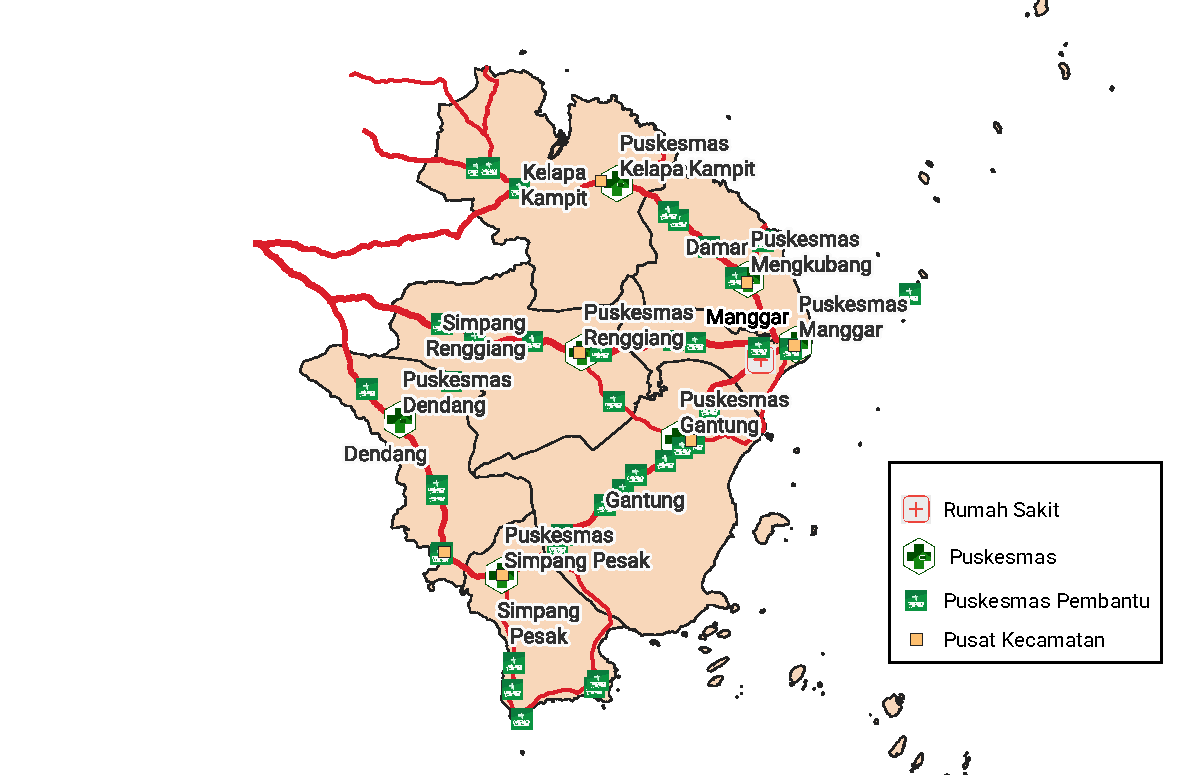
\includegraphics[width=\textwidth]{bab_02/bab_02_01_petaFaskes}	
	\caption{Lokasi Rumah Sakit, Puskesmas dan Puskesmas Pembantu di Kab. Belitung Timur}
	\label{fig:peta-puskesmas-rs}
\end{figure}

%\begin{sidewaysfigure}[ht]
%	\centering
%	%	maps better displayed in full width 
%	\includegraphics[width=\textwidth]{bab_02/rect5258}	
%	\caption{Lokasi Rumah Sakit, Puskesmas dan Puskesmas Pembantu di Kab. Belitung Timur}
%	\label{fig:peta-puskesmas-rs}
%\end{sidewaysfigure}

\subsection{Puskesmas Pembantu}
Puskesmas Pembantu merupakan jaringan pelayanan Puskesmas yang memberikan pelayanan kesehatan secara permanen di suatu lokasi dalam wilayah kerja Puskesmas\footnote{Permenkes No 75 Tahun 2014. pasal 40 ayat (2)}. Puskesmas  Pembantu merupakan bagian integral  Puskesmas, yang harus dibina secara berkala oleh Puskesmas.

Jumlah Puskesmas Pembantu di Kabupaten Belitung Timur pada tahun \tP adalah sebanyak 39 Pustu (\autoref{tab:Puskemas-dan-Pustu}).

\begin{table}[!ht]
\caption{Puskemas dan Jumlah Puskesmas Pembantu di Kab. Belitung Timur Tahun \tP}
\label{tab:Puskemas-dan-Pustu}
\centering{}%
\ra{1.3}

\begin{tabular}{lllr}
	\toprule
	No                    & Kecamatan         & Puskesmas     & Jumlah Puskesmas Pembantu \\
	\midrule
	1.                    & Manggar           & Manggar       &                         9 \\
	\rowcolor{black!10}2. & Damar             & Mengkubang    &                         5 \\
	3.                    & Gantung           & Gantung       &                         6 \\
	\rowcolor{black!10}4. & Kelapa Kampit     & Kelapa Kampit &                         7 \\
	5.                    & Simpang Renggiang & Renggiang     &                         4 \\
	\rowcolor{black!10}6. & Simpang Pesak     & Simpang Pesak &                         4 \\
	7.                    & Dendang           & Dendang       &                         4 \\
	\midrule
	       \multicolumn{2}{c}{Jumlah}         & 7             &                        39 \\
	\bottomrule
\end{tabular}
\end{table}

\section{AKSES DAN MUTU PELAYANAN KESEHATAN}
\subsection{Kunjungan Rawat Jalan dan Rawat Inap}
Kunjungan rawat jalan adalah kunjungan ke fasilitas pelayanan kesehatan tingkat pertama dan fasilitas pelayanan kesehatan rujukan tingkat lanjut milik pemerintah dan swasta untuk mendapatkan pelayanan kesehatan perseorangan yang meliputi observasi, diagnosa, pengobatan, rehabilitasi medik tanpa tinggal di ruang rawat inap untuk pertama kalinya dalam satu tahun tertentu. Kunjungan rawat jalan puskesmas termasuk kunjungan ke jaringan puskesmas, dalam gedung maupun luar gedung (puskesmas keliling, puskemas pembantu, bidan desa, pemeriksaan anak sekolah, dsb).
Kunjungan rawat inap adalah kunjungan ke fasilitas pelayanan kesehatan tingkat pertama dan fasilitas pelayanan kesehatan rujukan tingkat lanjut milik pemerintah dan swasta untuk mendapatkan pelayanan kesehatan perseorangan yang meliputi observasi, diagnosa, pengobatan, rehabilitasi medik, dan tinggal di ruang rawat inap untuk pertama kalinya dalam satu tahun tertentu.

Pada tahun \tP tercatat sebanyak 270.775 kunjungan di fasilitas layanan kesehatan di Kabupaten Belitung Timur. Sebanyak 196.087 kunjungan adalah ke fasilitas kesehatan milik pemerintah, sedangkan kunjungan ke fasilitas kesehatan milik swasta adalah sebanyak 74.688 kunjungan (\autoref{fig:Kunjungan-Faskes}).

Pada tahun \tP tercatat sebanyak 257.469 kali kunjungan rawat jalan dan 13.306 kunjungan rawat inap di fasilitas layanan kesehatan di Kabupaten Belitung Timur. Berdasarkan tingkat fasyankes, sebanyak 220.900 kunjungan adalah di Fasilitas Kesehatan Tingkat Pertama, sedangkan kunjungan di Fasilitas Kesehatan Tingkat Lanjutan adalah sebanyak 49.875 kunjungan (\autoref{fig:Kunjungan-Rawat}).

\begin{figure}[!htb]
    \centering{}
    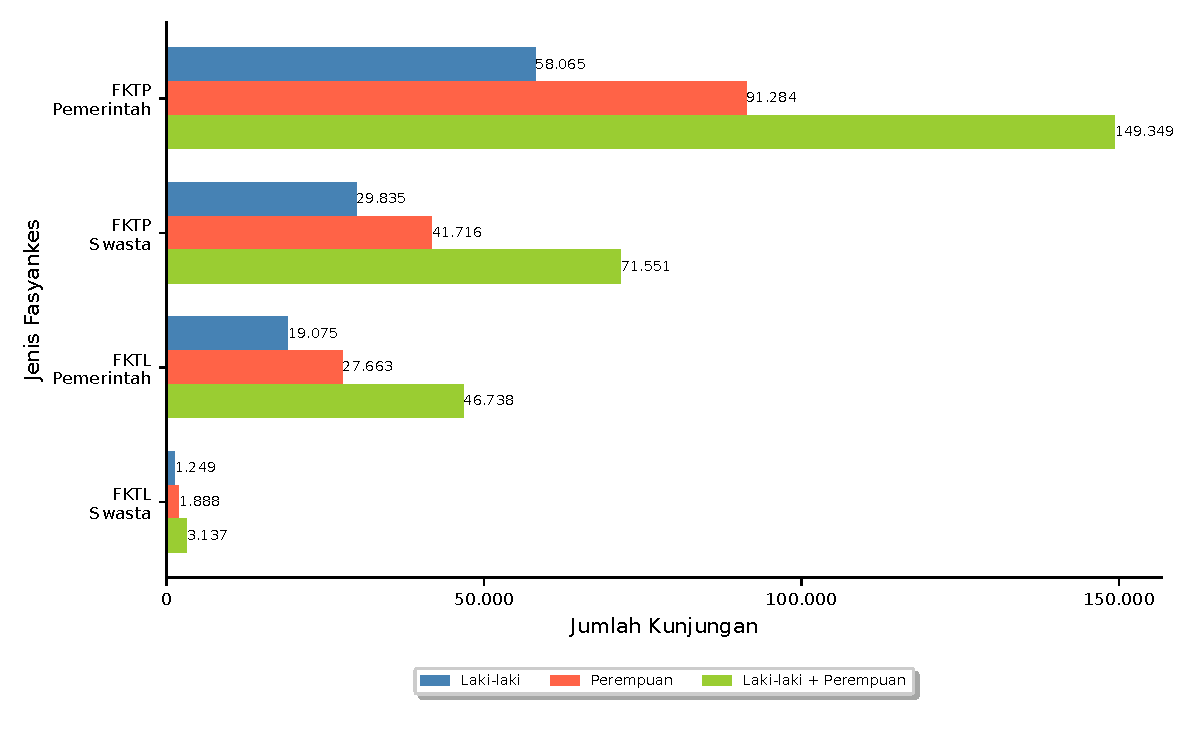
\includegraphics[width=0.9\textwidth]{bab_02/bab_02_1_kunjunganFaskes}
    \caption{Kunjungan Pasien Berdasarkan Jenis Faskes di Kab. Belitung Timur Tahun \tP}
    \label{fig:Kunjungan-Faskes}
\end{figure}

\begin{figure}[!htb]
    \centering{}
    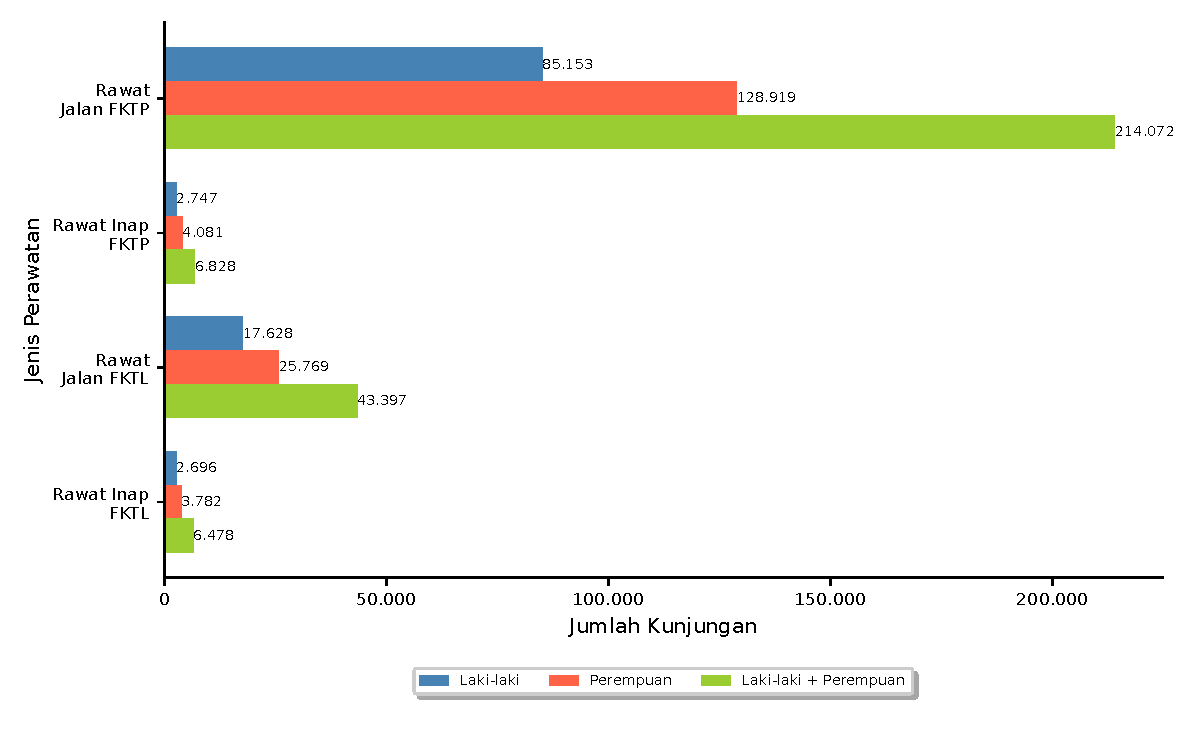
\includegraphics[width=0.9\textwidth]{bab_02/bab_02_2_rawat}
    \caption{Kunjungan Pasien Berdasarkan Jenis Perawatan di Kab. Belitung Timur Tahun \tP}
    \label{fig:Kunjungan-Rawat}
\end{figure}

\subsection{Kinerja Pelayanan Rumah Sakit}
Kinerja pelayanan rumah sakit dapat dinilai berdasarkan beberapa indikator, antara lain:
\begin{itemize}
 \item \emph{Gross Death Rate}(GDR), yaitu angka kematian umum untuk tiap-tiap 1.000 pasien keluar;
 \item \emph{Net Death Rate} (NDR), yaitu angka kematian ≥ 48 jam setelah dirawat untuk tiap-tiap 1.000 pasien keluar;
 \item \emph{Bed Occupancy Rate} (BOR), yaitu persentase pemakaian tempat tidur pada satu-satuan waktu tertentu;
 \item \emph{Bed Turn Over} (BTO), yaitu frekuensi pemakaian tempat tidur pada satu periode, berapa kali tempat tidur dipakai dalam satu satuan waktu;
 \item \emph{Turn Over Interval} (TOI), yaitu rata-rata hari tempat tidur tidak ditempati dari saat terisi ke saat terisi berikutnya; dan
 \item \emph{Average Length of Stay} (ALOS), yaitu rata-rata lama rawat (dalam satuan hari) seorang pasien.
\end{itemize}

Kinerja pelayanan rumah sakit di Kabupaten Belitung Timur pada tahun \tP dirangkum pada \autoref{tab:Kinerja-RS}.

\begin{table}[!ht]
\caption{Kinerja Pelayanan Rumah Sakit di Kab. Belitung Timur Tahun \tP}
\label{tab:Kinerja-RS}
\centering{}%
\ra{1.3}

\begin{tabular}{rlrr}
	\toprule
	                   No & Indikator                     &     Cakupan \tP &       Kondisi Ideal \\ 
	\midrule
	                   1. & \emph{Gross Death Rate}       & 48,39 per 1.000 & $\leq$ 45 per 1.000 \\
	\rowcolor{black!10}2. & \emph{Net Death Rate}         & 22,09 per 1.000 & $\leq$ 25 per 1.000 \\
	                   3. & \emph{Bed Occupancy Rate}     &         54,41\% &         60\% - 80\% \\
	\rowcolor{black!10}4. & \emph{Bed Turn Over}          &      58,43 kali &        40 - 50 kali \\
	                   5. & \emph{Turn Over Interval}     &       2,85 hari &          1 - 3 hari \\
	\rowcolor{black!10}6. & \emph{Average Length of Stay} &       3,40 hari &          6 - 9 hari \\ 
	\bottomrule
\end{tabular}
\end{table}

\subsection{Ketersediaan Obat Esensial dan Vaksin IRL}

Obat esensial adalah 40 item obat indikator yang merupakan obat pendukung Program Kesehatan Ibu dan Anak, Program Gizi, Program TB Paru, Program Malaria, serta obat pelayanan kesehatan dasar esensial dan terdapat di dalam Formularium Nasional. Vaksin Imunisasi Rutin Lengkap (IRL) terdiri dari jenis vaksin yang merupakan vaksin pendukung program imunisasi dasar, yaitu Hepatitis B, DPT-HB-HIB (Pentavac, Pentavalent (Easyfive), dan/ atau Vaksin ComBE Five), BCG, MR (Rubella), Polio (b-OPV dan/ atau IPV), PCV dan Rotavirus.

Persentase Puskesmas dengan ketersediaan obat esensial dan vaksin IRL adalah persentase Puskesmas yang memiliki ketersediaan minimal 90\% dari 40 item obat indikator serta 7 vaksin IRL pada saat dilakukan pemantauan terhadap seluruh puskesmas yang melaporkan data. Laporan yang disampaikan yaitu laporan pada bulan November atau laporan bulan terakhir pada tahun pelaporan.

Pada tahun \tP terdapat 100\% Puskesmas yang memenuhi ketersediaan obat esensial dan vaksin IRL di Kabupaten Belitung Timur.

\section[UKBM]{UPAYA KESEHATAN BERSUMBERDAYA MASYARAKAT (UKBM)}% for title and page
\sectionmark{UKBM} %for header
\subsection{Posyandu}
Posyandu adalah salah satu bentuk Upaya Kesehatan Bersumberdaya Masyarakat (UKBM) yang dikelola dan diselenggarakan dari, oleh, untuk, dan bersama masyarakat guna memberdayakan masyarakat dan memberikan kemudahan kepada masyarakat dalam memperoleh pelayanan kesehatan dasar untuk mempercepat penurunan angka kematian ibu, bayi, dan balita. Posyandu melayani kegiatan berupa penimbangan bayi dan balita, pemberian imunisasi, konsultasi kesehatan dan Pemberian Makanan Tambahan (PMT).

Jumlah Posyandu di Kabupaten Belitung Timur tahun \tP adalah sebanyak 134 posyandu aktif dari total 134 unit posyandu (\autoref{fig:Posyandu-Aktif}).

\begin{figure}[H]
	\centering{}
	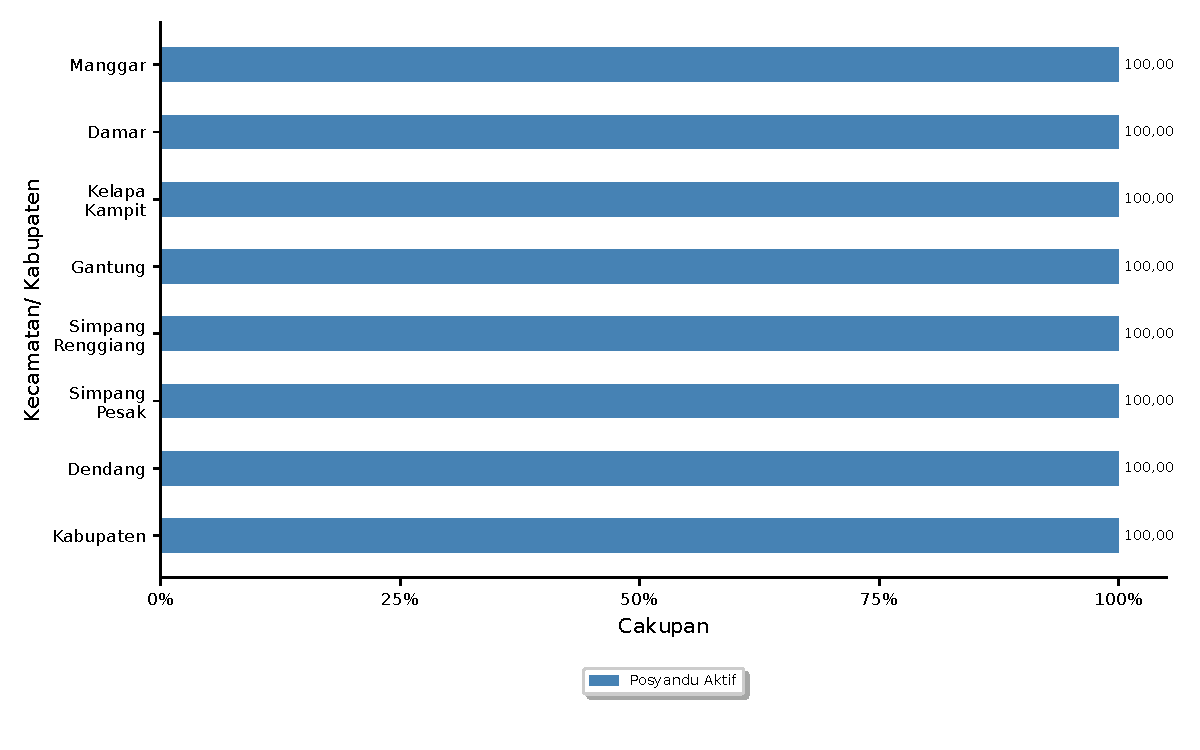
\includegraphics[width=0.9\textwidth]{bab_02/bab_02_3_posyandu}
	\caption{Persentase Posyandu Aktif di Kab. Belitung Timur Tahun \tP}
	\label{fig:Posyandu-Aktif}
\end{figure}

%\subsection{Posbindu PTM}
%Posbindu PTM adalah suatu upaya kesehatan berbasis bersumberdaya masyarakat (UKBM) dalam pencegahan dan pengendalian Penyakit Tidak Menular (PTM) melalui kegiatan skrining kesehatan/ deteksi dini faktor risiko PTM, intervensi/ modifikasi faktor risiko PTM serta monitoring dan tindak lanjut faktor risiko PTM bersumber daya masyarakat secara rutin dan berkesinambungan.
%
%Jumlah Posbindu PTM di Kabupaten Belitung Timur tahun \tP adalah sebanyak 58 Posbindu PTM. %(\autoref{tab:Posyandu-Posbindu-di-Kab}).

%\cleardoublepage
%\include{bab_03/bab_03_sumber_daya_manusia_kesehatan} % done
%\cleardoublepage
%\include{bab_04/bab_04_pembiayaan_kesehatan} %done
%\cleardoublepage
%\chapter{KESEHATAN KELUARGA}

Pembangunan keluarga dilakukan dalam upaya untuk mewujudkan keluarga berkualitas yang hidup dalam lingkungan yang sehat. Selain lingkungan yang sehat, kondisi kesehatan dari tiap anggota keluarga sendiri juga merupakan salah satu syarat dari keluarga yang berkualitas.
Keluarga berperan terhadap optimalisasi pertumbuhan, perkembangan, dan produktivitas seluruh anggotanya melalui pemenuhan kebutuhan gizi dan menjamin kesehatan anggota keluarga. 

Di dalam komponen keluarga, ibu dan anak merupakan kelompok rentan terhadap keadaan keluarga dan sekitarnya secara umum.
Hal ini terkait dengan fase kehamilan, persalinan dan nifas pada ibu dan fase tumbuh kembang pada anak.
Oleh karena itu ibu dan anak merupakan anggota keluarga yang perlu mendapatkan prioritas dalam penyelenggaraan upaya kesehatan.

\section{KESEHATAN IBU}
Seorang ibu mempunyai peranan yang sangat penting dalam pertumbuhan anak dan bayi.
Hal ini terkait dengan fase kehamilan, persalinan dan nifas pada ibu dan fase tumbuh kembang pada anak.
Gangguan kesehatan yang dialami pada seorang ibu dapat mempengaruhi kesehatan janin dalam kandungan hingga kelahiran dan masa pertumbuhan bayi dan anaknya.

\subsection{Angka Kematian Ibu (AKI)}
Kematian ibu adalah kematian yang terjadi pada seorang ibu yang terjadi karena peristiwa kehamilan, persalinan, dan masa nifas (dalam kurun waktu 42 hari sejak terminasi kehamilan) tanpa memandang lamanya kehamilan, yakni kematian yang disebabkan karena kehamilannya atau penanganannya, tetapi bukan karena sebab-sebab lain seperti kecelakaan dan terjatuh.
Angka Kematian Ibu (AKI) menggambarkan status gizi dan tingkat pelayanan kesehatan terhadap ibu hamil, ibu melahirkan dan ibu masa nifas.

Jumlah Kematian Ibu di Kabupaten Belitung Timur pada tahun \tP adalah 4 orang, dengan Angka Kematian Ibu (AKI) 240,53 per 100.000 kelahiran hidup (\autoref{fig:Jumlah-Kematian-Ibu}). 

\begin{figure}[H]
    \centering{}
    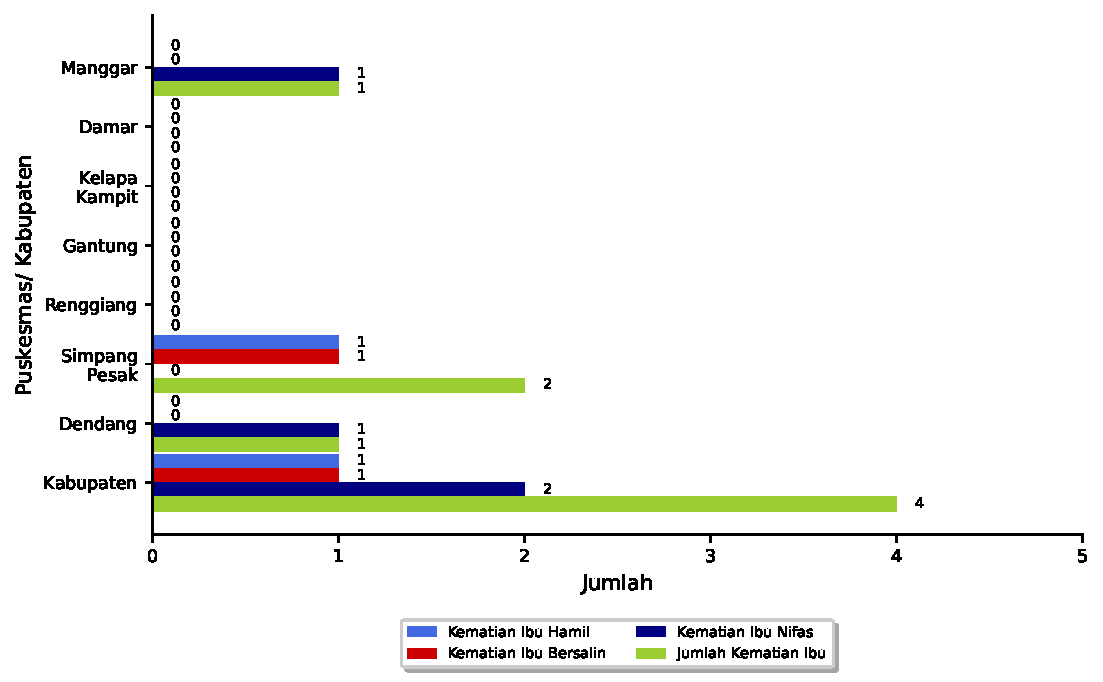
\includegraphics[width=0.9\textwidth]{bab_05/bab_05_01_kematianIbu}
    \caption{Jumlah Kematian Ibu di Kab. Belitung Timur Tahun \tP per Puskesmas}
    \label{fig:Jumlah-Kematian-Ibu}
\end{figure}

\begin{figure}[H]
    \centering{}
    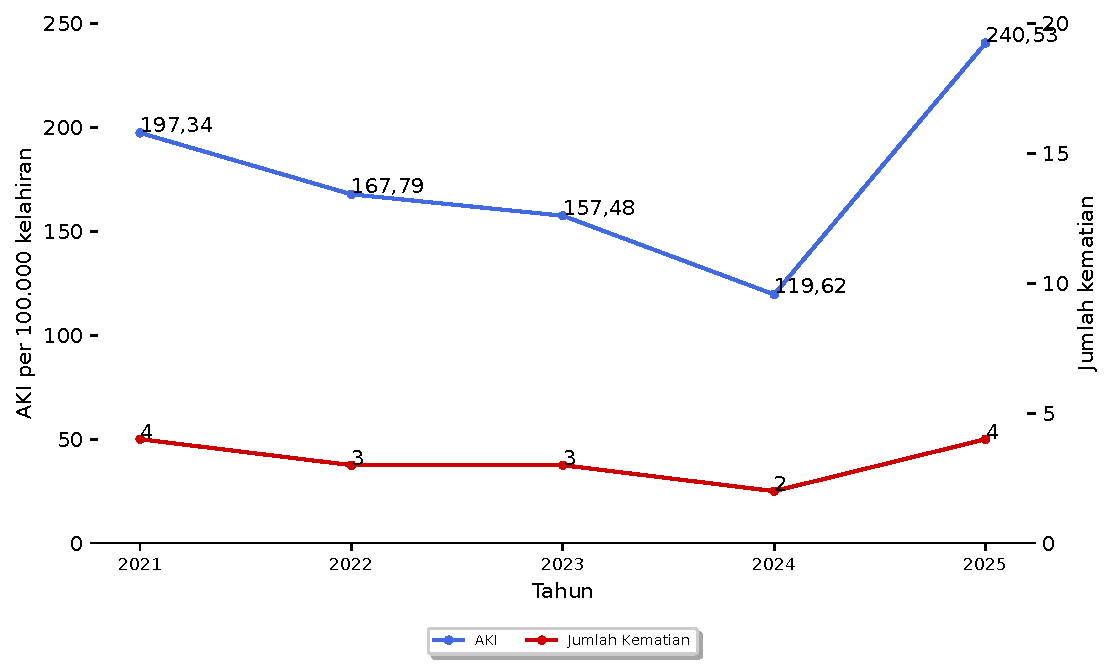
\includegraphics[width=0.85\textwidth]{bab_05/bab_05_02_plotAKI}
    \caption{AKI Kab. Belitung Timur \tPlot}
    \label{fig:AKI-2021-2025}
\end{figure}

\subsection{Pelayanan Antenatal (K1 dan K6)}
Cakupan kunjungan ibu hamil K-1 adalah cakupan kunjungan ibu hamil yang mendapat pelayanan antenatal sesuai standar (10T) oleh tenaga kesehatan pada masa kehamilan trimester
pertama di satu wilayah kerja pada kurun waktu tertentu. Cakupan ibu hamil K6 adalah cakupan ibu hamil yang mendapatkan pelayanan antenatal sesuai standar (10T) paling sedikit enam kali, dengan distribusi pemberian pelayanan yang dianjurkan adalah minimal satu kali pada trimester pertama, dua kali pada trimester kedua dan tiga kali pada trimester ketiga dengan paling sedikit 2 kali oleh dokter pada trimester pertama dan ketiga.

Cakupan K1 dan K6 di Kabupaten Belitung Timur pada tahun \tP adalah sebesar 97,18\% dan 84,09\% (\autoref{fig:Cakupan-K1-K6})

\begin{figure}[H]
    \centering{}
    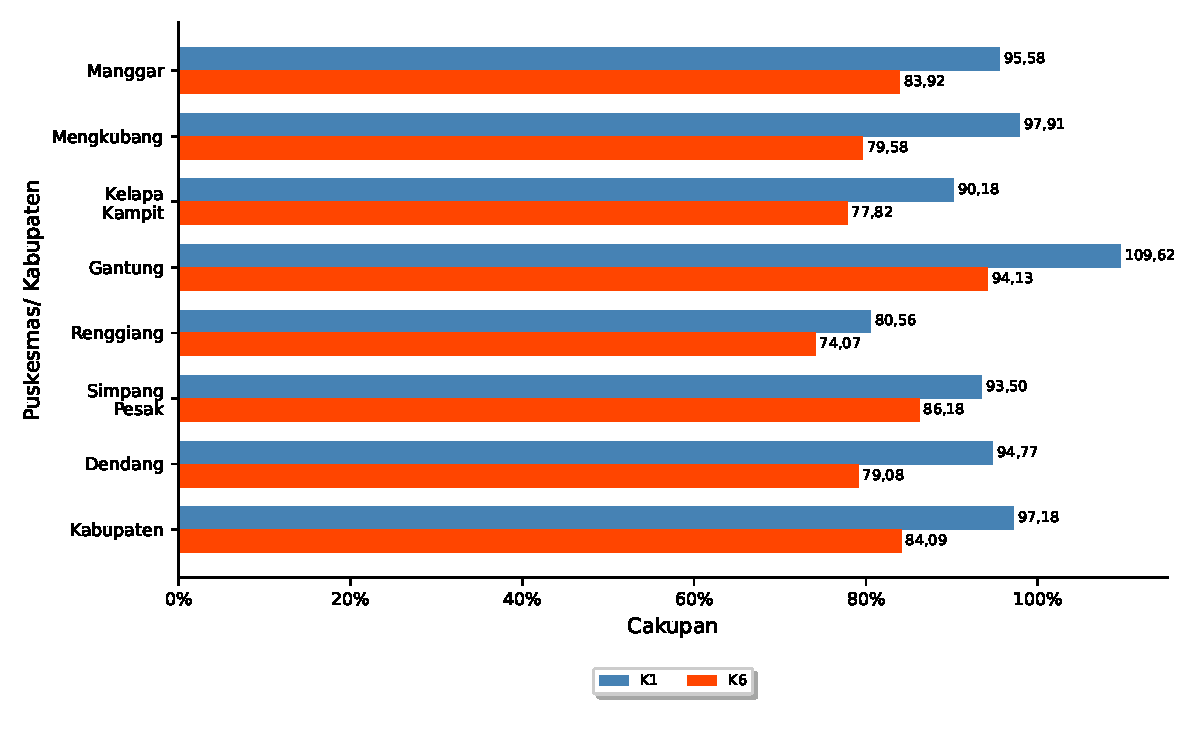
\includegraphics[width=0.9\textwidth]{bab_05/bab_05_03_K1K6}
    \caption{Cakupan K1 dan K6 di Kab. Belitung Timur Tahun \tP per Puskesmas}
    \label{fig:Cakupan-K1-K6}
\end{figure}

% not enough data for five-year plot
%\begin{figure}[H]
%    \centering{}
%    \includegraphics[width=0.85\textwidth]{bab_05/bab_05_03a_plotK1K6}
%    \caption{Cakupan K1 dan K6 di Kab. Belitung Timur Tahun \tPlot}
%    \label{fig:Cakupan-K1-K6-\tPlotFig}
%\end{figure}


\subsection{Imunisasi Td Ibu Hamil}
Peraturan Menteri Kesehatan Nomor 42 Tahun 2013 tentang Penyelenggaraan Imunisasi mengamanatkan bahwa wanita usia subur dan ibu hamil merupakan salah satu kelompok populasi yang menjadi sasaran imunisasi lanjutan.
Imunisasi lanjutan adalah kegiatan yang bertujuan untuk melengkapi imunisasi dasar pada bayi yang diberikan kepada anak batita, anak usia sekolah, dan wanita usia subur termasuk ibu hamil.
Salah satu upaya imunisasi lanjutan yang menyasar ibu hamil adalah imunisasi Td untuk mengendalikan infeksi tetanus yang merupakan salah satu faktor risiko kematian ibu dan kematian bayi.
Infeksi tetanus disebabkan oleh bakteri \emph{Clostridium tetani} sebagai akibat dari proses persalinan yang tidak aman/ steril atau berasal dari luka yang diperoleh ibu hamil sebelum melahirkan.

Cakupan Imunisasi Td pada ibu hamil adalah ang mendapatkan imunisasi Td (Tetanus difteri) dengan interval tertentu (yang dimulai saat dan atau sebelum kehamilan) dengan memperhatikan hasil skrining dan status T.

Cakupan Td5 ibu hamil di kabupaten Belitung Timur tahun \tP yaitu sebesar 41,91\%, sedangkan cakupan Td2+ yaitu sebesar 48,21\% (\autoref{fig:Cakupan-Td}).

\begin{figure}[H]
    \centering{}
    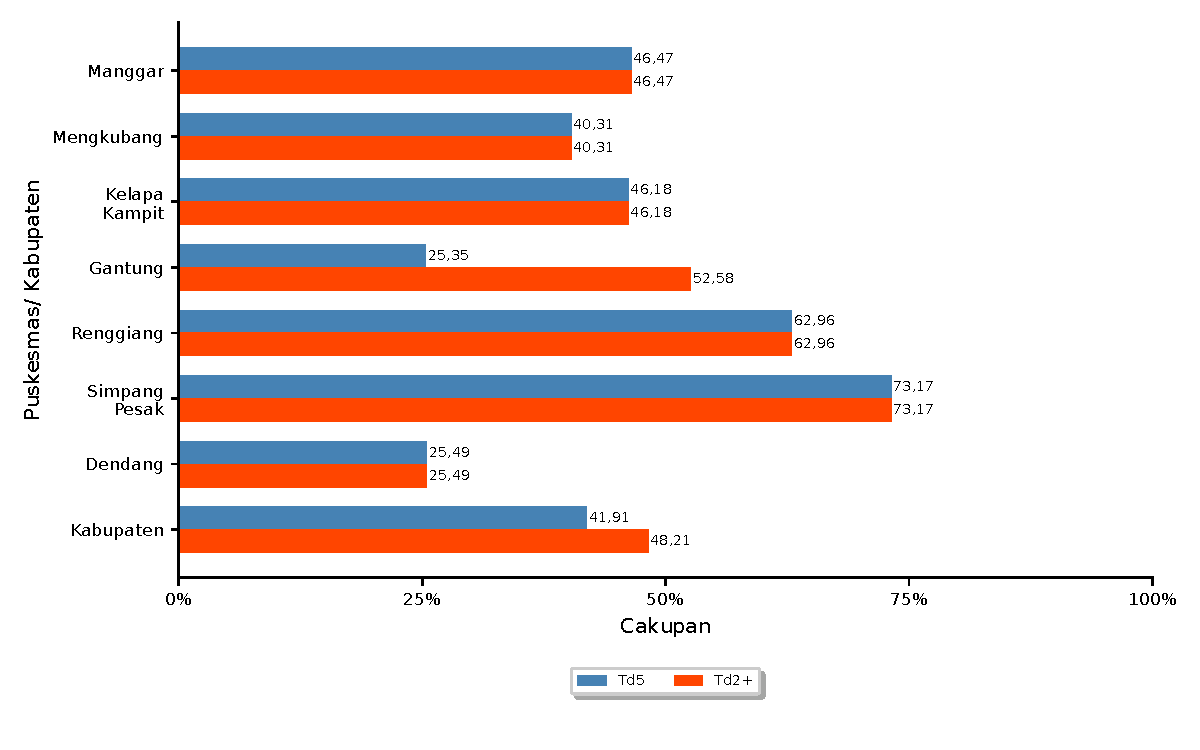
\includegraphics[width=0.85\textwidth]{bab_05/bab_05_04_Td}
    \caption{Cakupan Imunisasi Td Ibu Hamil di Kab. Belitung Timur Tahun \tP per Puskemas}
    \label{fig:Cakupan-Td}
\end{figure}

\subsection{Pemberian Tablet Tambah Darah}
Salah satu komponen pelayanan kesehatan ibu hamil yaitu pemberian suplemen zat besi sebanyak 90 tablet (Fe3).
Zat besi merupakan mineral yang dibutuhkan tubuh untuk membentuk sel darah merah (hemoglobin).
Zat besi memiliki peran vital terhadap pertumbuhan janin.
Selama hamil, asupan zat besi harus ditambah mengingat selama kehamilan, volume darah pada tubuh ibu meningkat.
Sehingga, untuk dapat tetap memenuhi kebutuhan ibu dan menyuplai makanan serta oksigen pada janin melalui plasenta, dibutuhkan asupan zat besi yang lebih banyak.

Cakupan ibu hamil mendapat TTD adalah persentase ibu hamil yang mendapatkan Tablet Tambah Darah (TTD) sekurangnya mengandung zat besi setara dengan 60 mg besi elemental dan 0,4 mg asam folat yang disediakan oleh pemerintah minimal 90 tablet selama masa kehamilan. Cakupan ibu hamil mengonsumsi TTD adalah persentase ibu hamil yang mengonsumsi Tablet Tambah Darah (TTD) sekurangnya mengandung zat besi setara dengan 60 mg besi elemental dan 0,4 mg asam folat yang disediakan oleh pemerintah minimal 90 tablet selama masa kehamilan.

Cakupan ibu hamil mendapat TTD di Kabupaten Belitung Timur pada tahun \tP adalah sebesar 84,09\% (\autoref{fig:Cakupan-TTD}).

\begin{figure}[H]
    \centering
    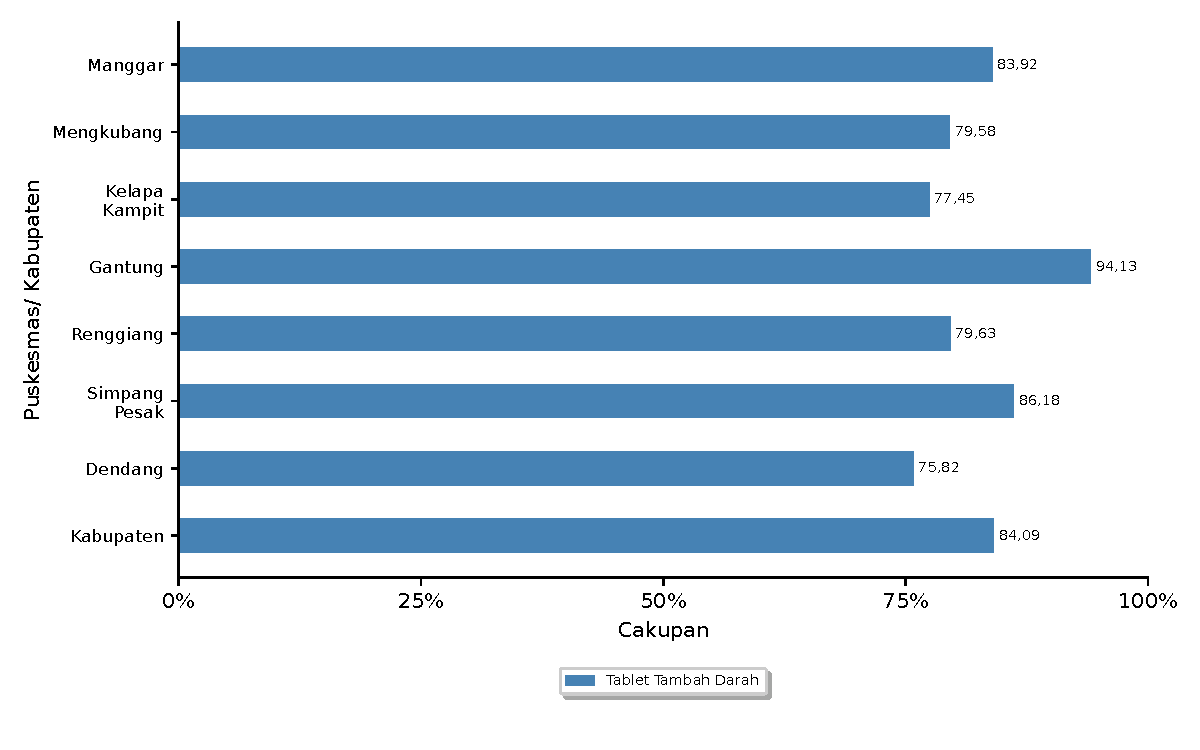
\includegraphics[width=0.9\textwidth]{bab_05/bab_05_05_TTD}
    \caption{Cakupan Pemberian TTD di Kab. Belitung Timur Tahun \tP per Puskesmas}
    \label{fig:Cakupan-TTD}
\end{figure}


\subsection{Pertolongan Persalinan oleh Tenaga Kesehatan dengan Kompetensi Kebidanan}
Salah satu upaya menekan angka kematian ibu dan bayi yaitu dengan mendorong upaya persalinan dilakukan oleh tenaga kesehatan dengan kompetensi kebidanan di fasilitas pelayanan kesehatan.

Cakupan persalinan di fasilitas pelayanan kesehatan adalah cakupan ibu bersalin yang mendapatkan pelayanan persalinan sesuai standar di fasilitas pelayanan kesehatan di satu wilayah kerja pada kurun waktu tertentu.

Cakupan persalinan di fasilitas pelayanan kesehatan di Kabupaten Belitung Timur pada tahun \tP yaitu sebesar 90,50\% (\autoref{fig:Cakupan-Persalinan-Fasyankes}).

\begin{figure}[H]
    \centering
    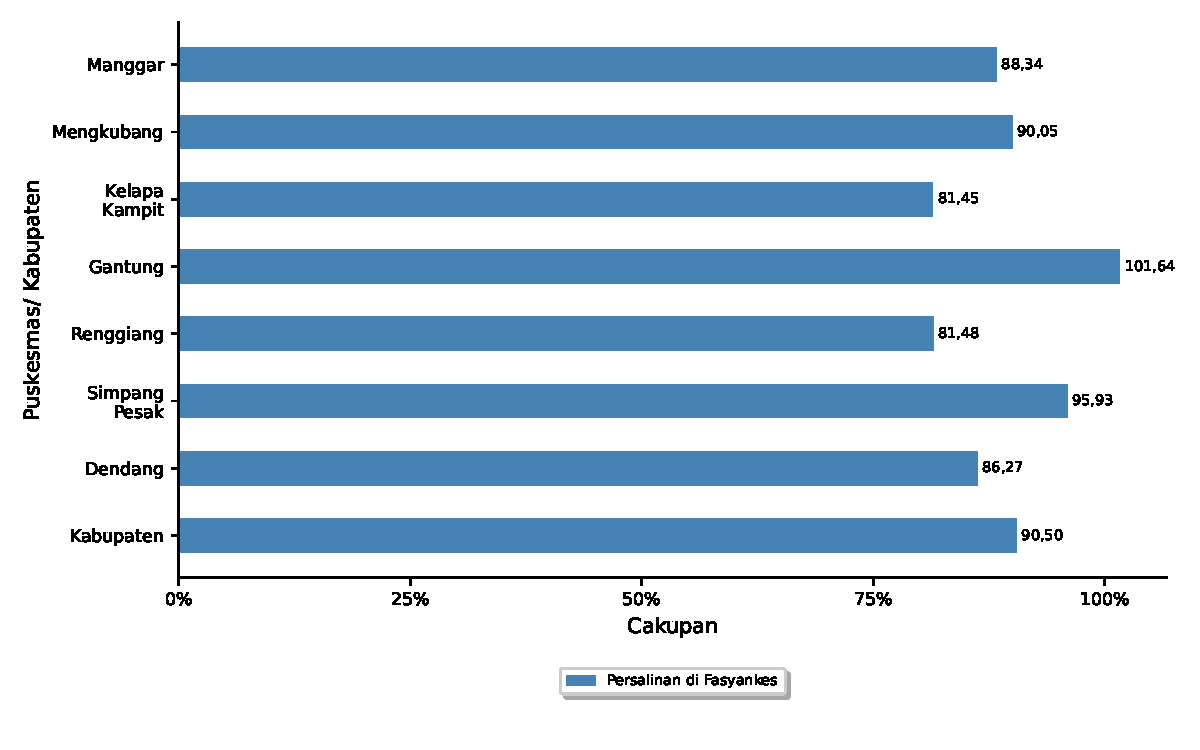
\includegraphics[width=0.9\textwidth]{bab_05/bab_05_05b_salinFasyankes.pdf}
    \caption{Cakupan Persalinan di Fasyankes di Kab. Belitung Timur Tahun \tP per Puskesmas}
    \label{fig:Cakupan-Persalinan-Fasyankes}
\end{figure}

\subsection{Pelayanan Kesehatan Nifas}
Masa nifas dimulai dari enam jam sampai dengan 42 hari pasca persalinan.
Pelayanan kesehatan nifas adalah pelayanan kepada ibu nifas sesuai standar sedikitnya 3 kali, yaitu kunjungan nifas ke-1 pada 6 jam setelah persalinan s.d 3 hari; kunjungan nifas ke-2 hari ke 4 s/d hari ke 28 setelah persalinan, kunjungan nifas ke-3 hari ke 29 s/d hari ke 42 setelah persalinan.

Cakupan pelayanan nifas KF Lengkap adalah cakupan pelayanan kepada ibu pada masa 6 jam sampai dengan 42 hari pasca bersalin sesuai standar paling sedikit 4 kali dengan distribusi waktu 6 jam sampai hari ke-2 (KF1), hari ke-3 sampai hari ke-7 (KF2), hari ke 8 sampai ke-28 (KF3) dan hari ke-29 sampai ke-42 (KF4) setelah bersalin di suatu wilayah kerja pada kurun waktu tertentu.

Cakupan pelayanan kesehatan nifas di Kabupaten Belitung Timur pada tahun \tP sebesar 88,38\% (\autoref{fig:Cakupan-Yankes-Nifas}).

\begin{figure}[H]
    \centering{}
    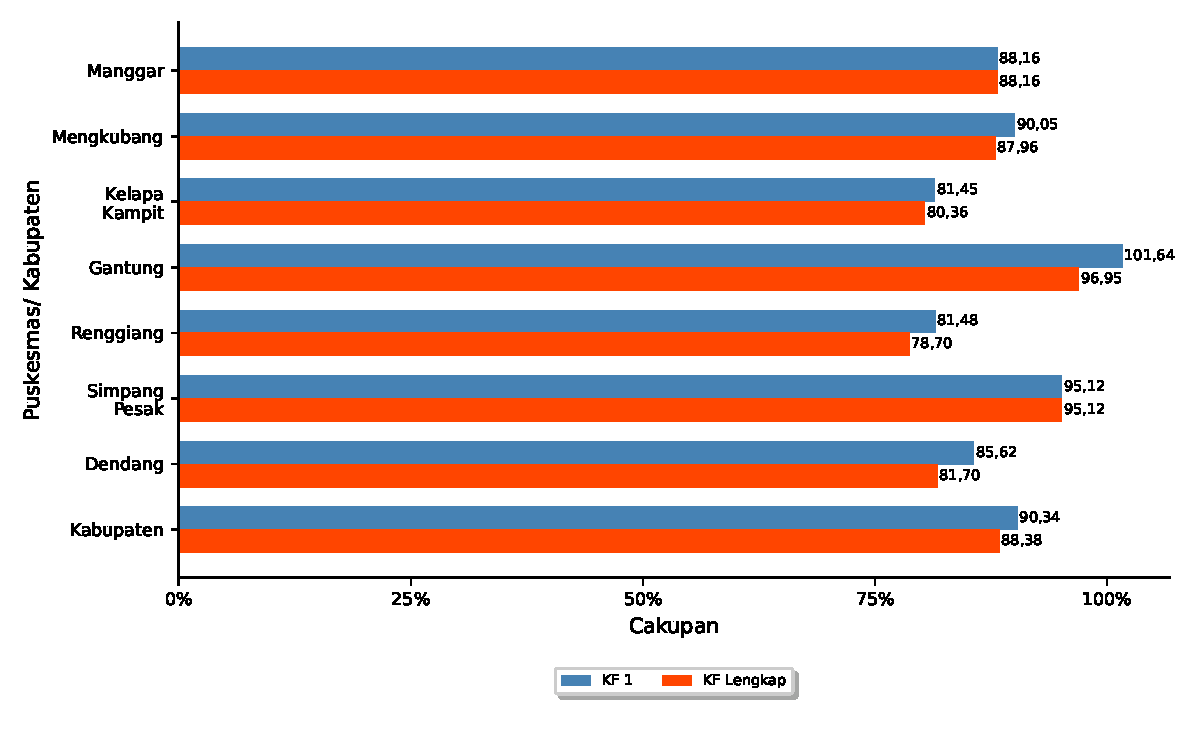
\includegraphics[width=0.9\textwidth]{bab_05/bab_05_05c_layanNifas}
    \caption{Cakupan Pelayanan Kesehatan Nifas di Kab. Belitung Timur Tahun \tP per Puskesmas}
    \label{fig:Cakupan-Yankes-Nifas}
\end{figure}

Cakupan ibu nifas mendapat vitamin A adalah cakupan ibu yang baru melahirkan atau nifas yang mendapatkan kapsul vitamin A 200.000 SI sehingga bayinya akan memperoleh vitamin A melalui ASI di satu wilayah kerja pada kurun waktu tertentu.
Cakupan ibu nifas mendapat vitamin A di Kabupaten Belitung Timur pada tahun \tP sebesar 90,50\% (\autoref{fig:Cakupan-Nifas-VitA}).

\begin{figure}[H]
    \centering{}
    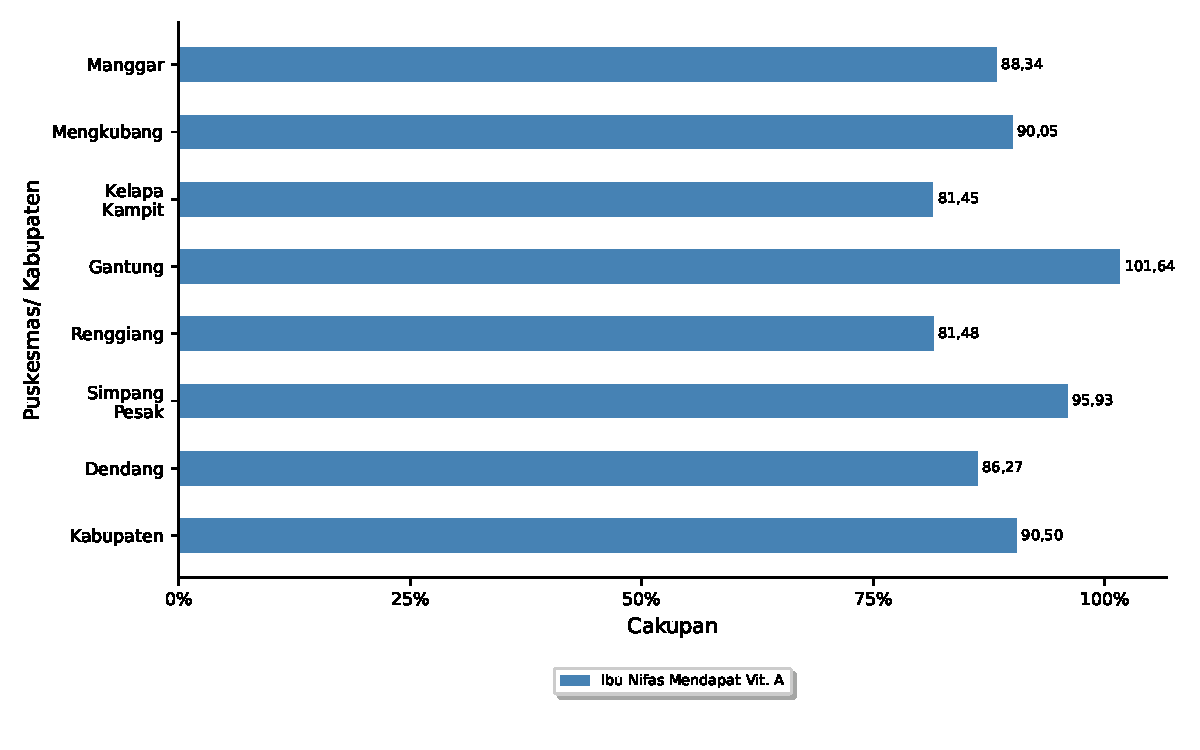
\includegraphics[width=0.9\textwidth]{bab_05/bab_05_05d_nifasVitA}
    \caption{Cakupan Ibu Nifas Mendapat Vitamin A di Kab. Belitung Timur Tahun \tP per Puskesmas}
    \label{fig:Cakupan-Nifas-VitA}
\end{figure}

\subsection{Penanganan Komplikasi Kebidanan}
Komplikasi kebidanan adalah kesakitan pada ibu hamil, ibu bersalin, ibu nifas yang dapat mengancam jiwa ibu dan/atau bayi. Sebagai salah satu faktor penyebab kematian ibu dan bayi, perlu dilakukan penanganan komplikasi kebidanan sebagai upaya menekan angka kematian ibu dan bayi.

Cakupan penanganan komplikasi kebidanan di Kabupaten Belitung Timur pada tahun \tP adalah sebesar 170,20\%,
%menurun dari cakupan tahun 2020 sebesar 133,97\% (\autoref{fig:Cakupan-Komplikasi-Kebidanan}).

\begin{figure}[H]
    \centering
    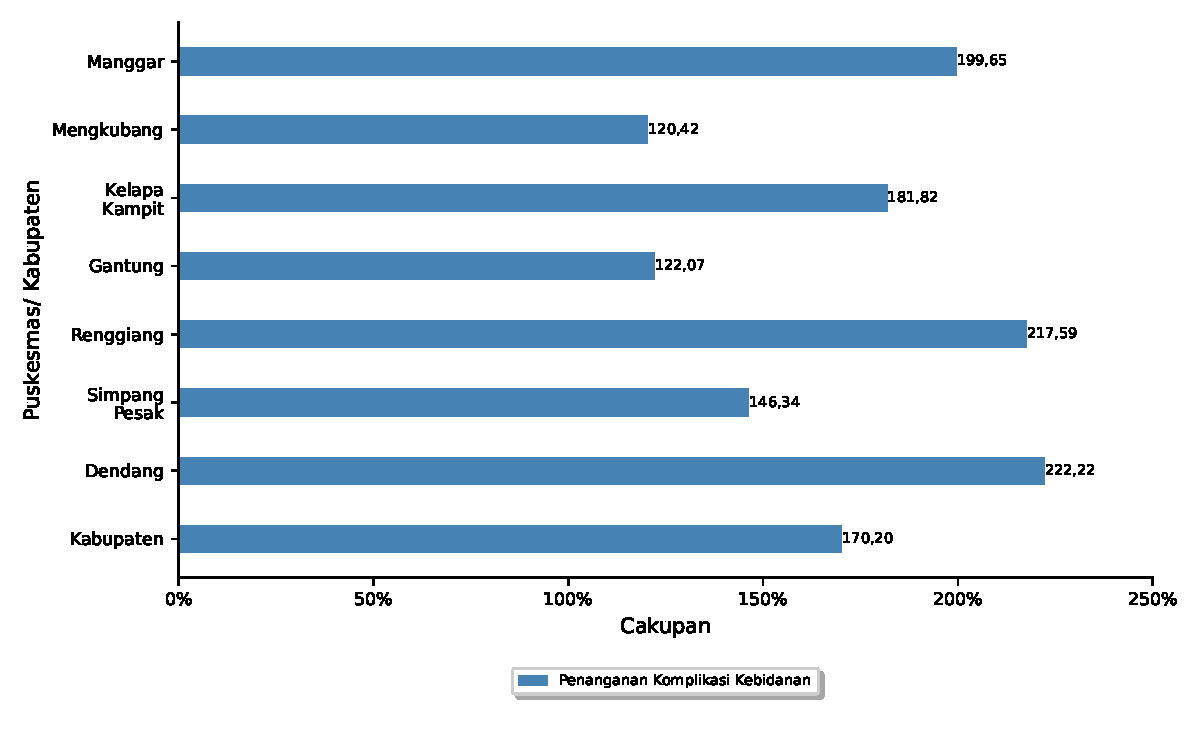
\includegraphics[width=0.9\textwidth]{bab_05/bab_05_05e_komplikasiKebidanan}
    \caption{Cakupan Penanganan Komplikasi Kebidanan di Kab. Belitung Timur Tahun \tP per Puskesmas}
    \label{fig:Cakupan-Komplikasi-Kebidanan}
\end{figure}


\subsection{Cakupan Peserta Keluarga Berencana}
Keluarga Berencana (KB) adalah upaya mengatur kelahiran anak, jarak dan usia ideal melahirkan, mengatur kehamilan, melalui promosi, perlindungan, dan bantuan sesuai dengan hak reproduksi untuk mewujudkan keluarga yang berkualitas. Program KB bertujuan untuk:
\begin{itemize}
 \item mengatur kehamilan yang diinginkan;
 \item menjaga kesehatan dan menurunkan angka kematian ibu, bayi dan anak;
 \item meningkatkan akses dan kualitas informasi, pendidikan, konseling, dan pelayanan keluarga berencana dan kesehatan reproduksi;
 \item meningkatkan partisipasi dan kesertaan pria dalam praktek keluarga berencana; dan
 \item mempromosikan penyusuan bayi sebagai upaya untuk menjarangkan jarak kehamilan.
\end{itemize}
Diharapkan dengan program KB akan dapat meningkatkan kualitas keluarga agar dapat timbul rasa aman, tenteram, dan harapan masa depan yang lebih baik dalam mewujudkan kesejahteraan lahir dan kebahagiaan batin.

\subsubsection{Cakupan peserta KB Aktif}
Peserta KB aktif adalah peserta KB baru dan lama yang masih aktif memakai kontrasepsi terus-menerus untuk menunda, menjarangkan kehamilan atau yang mengakhiri kesuburan. Cakupan peserta KB aktif di Kabupaten Belitung Timur pada tahun \tP adalah sebesar 85,61\% (\autoref{fig:Cakupan-KB-aktif-a} \& ~\autoref{fig:Cakupan-KB-aktif-b}). Metode KB yang paling banyak dipilih oleh peserta KB aktif adalah KB Suntik sebanyak 52,34 \% (\autoref{fig:Cakupan-KB-aktif-c}).

\begin{figure}[!htb]
    \centering
    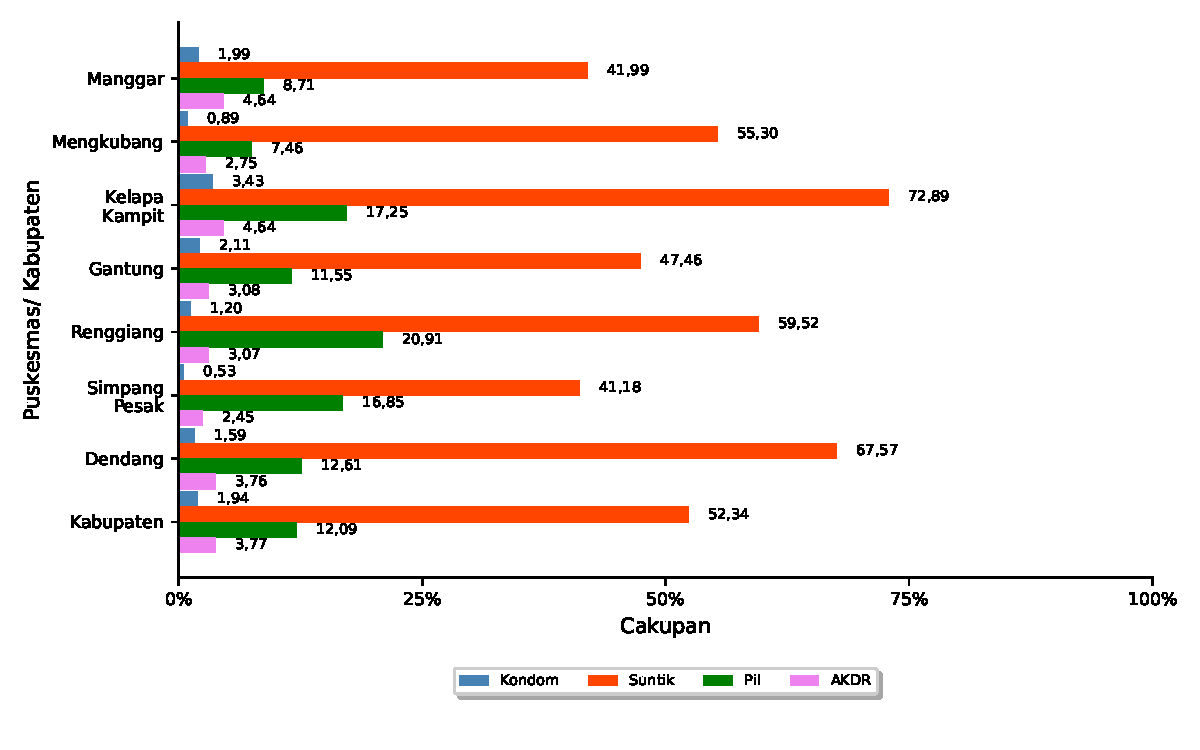
\includegraphics[width=0.9\textwidth]{bab_05/bab_05_06_KBaktif_a}
    \caption{Cakupan Peserta KB Aktif di Kab. Belitung Timur Tahun \tP per Puskesmas}
    \label{fig:Cakupan-KB-aktif-a}
\end{figure}

\begin{figure}[!htb]
    \centering
    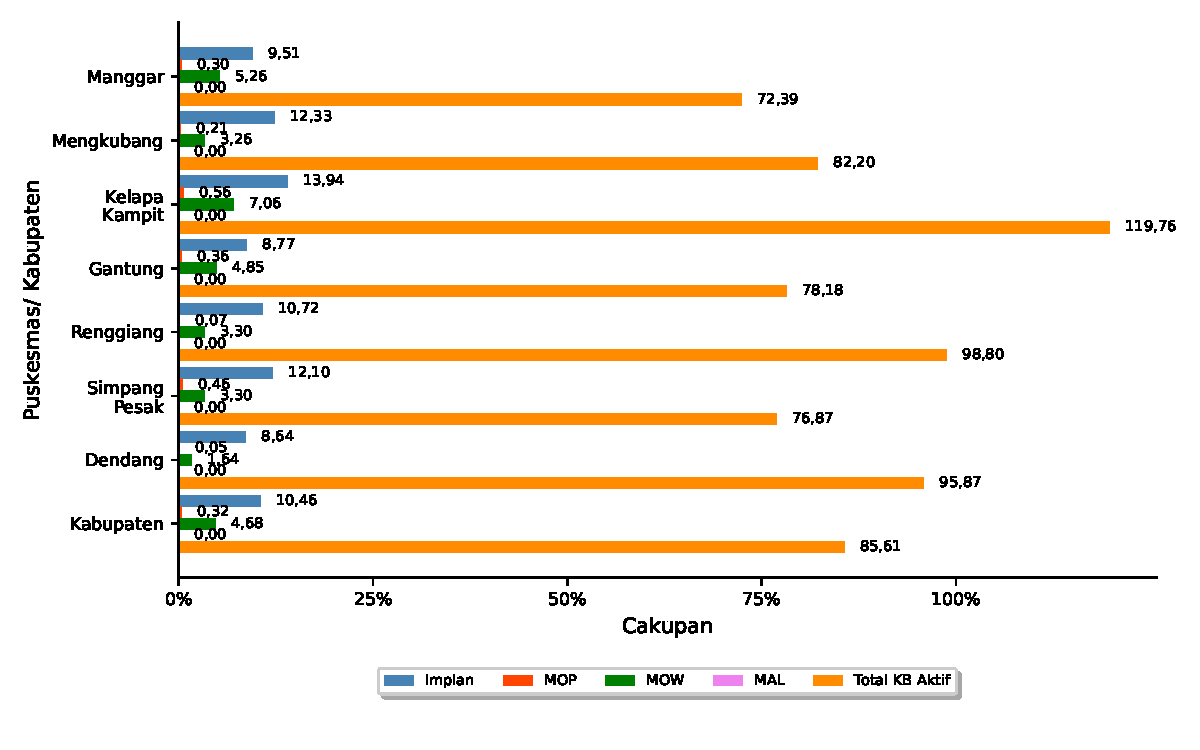
\includegraphics[width=0.9\textwidth]{bab_05/bab_05_06_KBaktif_b}
    \caption{Cakupan Peserta KB Aktif di Kab. Belitung Timur Tahun \tP per Puskesmas (lanj.)}
    \label{fig:Cakupan-KB-aktif-b}
\end{figure}

\begin{figure}[H]
    \centering
    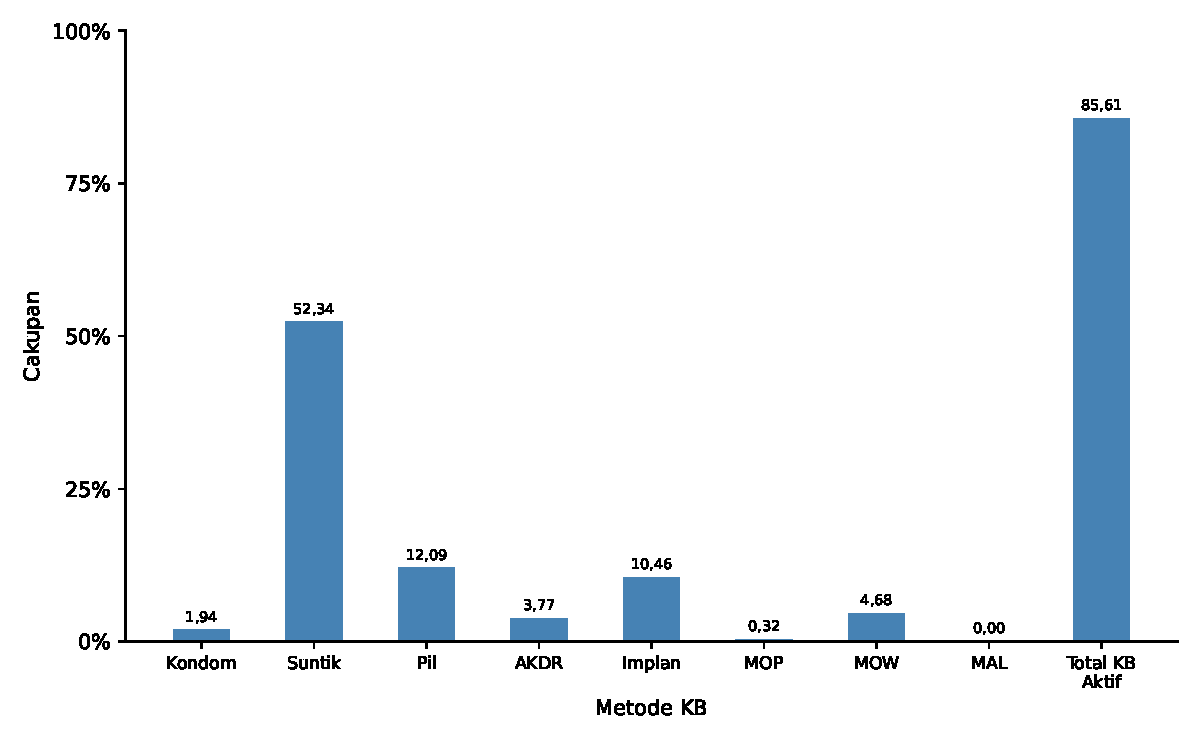
\includegraphics[width=0.9\textwidth]{bab_05/bab_05_06_KBaktif_c}
    \caption{Cakupan Metode Yang Digunakan Peserta KB Aktif di Kab. Belitung Timur Tahun \tP}
    \label{fig:Cakupan-KB-aktif-c}
\end{figure}

\subsubsection{Pasangan Usia Subur dengan status 4T dan ALKI}
Pasangan Usia Subur(PUS) dengan status 4 Terlalu (4T) adalah PUS dimana istrinya memenuhi minimal salah satu kriteria 4 Terlalu (4T), yaitu :
\begin{enumerate}
	\item berusia kurang dari 20 tahun;
	\item berusia lebih dari 35 tahun;
	\item telah memiliki anak hidup lebih dari 3 orang;atau
	\item jarak kelahiran antara satu anak dengan lainnya kurang dari 2 tahun
\end{enumerate}

Cakupan PUS dengan status 4T yang menjadi peserta KB aktif di Kabupaten Belitung Timur pada tahun \tP  adalah sebesar 64,19\% (\autoref{fig:Cakupan-4T-ALKI-menjadi-KB-Aktif}).

Pasangan Usia Subur(PUS) dengan ALKI adalah PUS yang istrinya mengalami salah satu dari gejala: Anemia, Lingkar Lengan Atas < 23,5, penyakit kronis, atau Infeksi Menular Seksual (IMS).
Penyakit kronis yang dimaksud terdiri dari Diabetes Melitus, Hipertensi, jantung, ginjal, auto imun, Hepatitis B, Thyroid, TORCH, hiperkoagulasi, stroke, Thalasemia, Hemofilia, kanker, masalah kesehatan jiwa, HIV, TBC, dan Malaria.

Cakupan PUS dengan ALKI yang menjadi peserta KB aktif di Kabupaten Belitung Timur pada tahun \tP  adalah sebesar 89,25\% (\autoref{fig:Cakupan-4T-ALKI-menjadi-KB-Aktif}).

\begin{figure}[H]
	\centering
	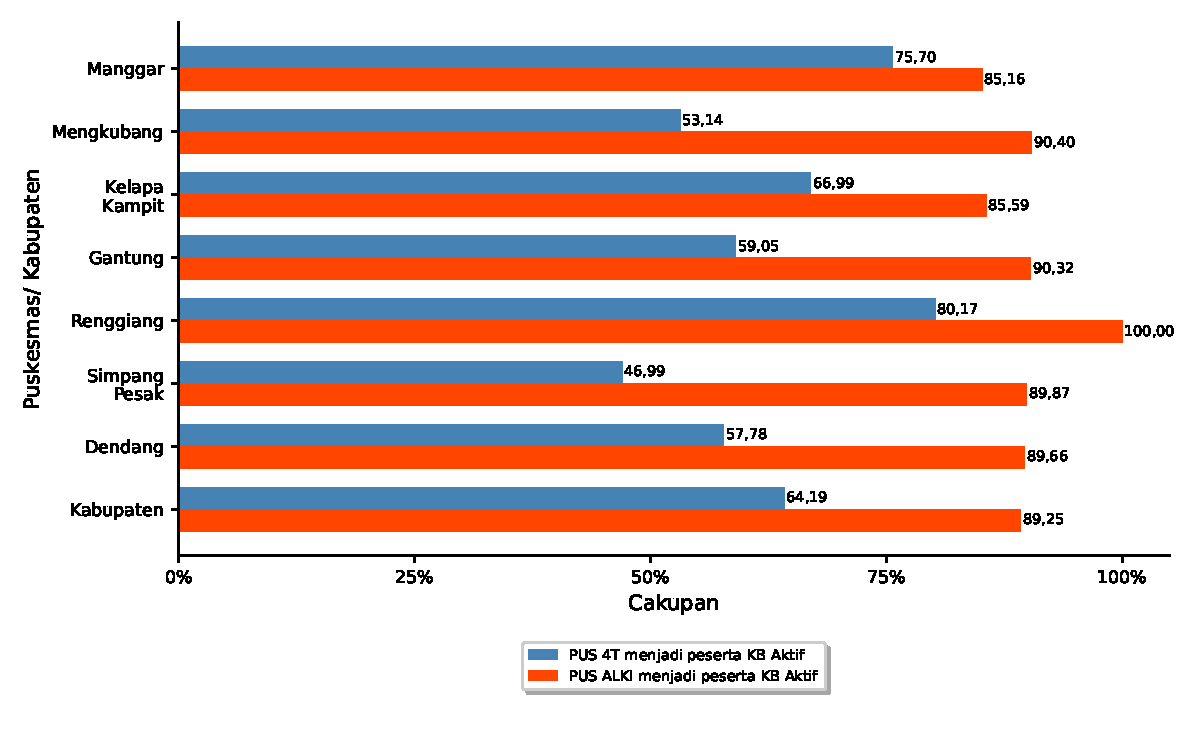
\includegraphics[width=0.9\textwidth]{bab_05/bab_05_06a_KB4TALKI}
	\caption{Cakupan PUS Dengan Status 4T dan ALKI Menjadi Peserta KB Aktif di Kab. Belitung Timur Tahun \tP}
	\label{fig:Cakupan-4T-ALKI-menjadi-KB-Aktif}
\end{figure}

\subsubsection{Cakupan peserta KB Pasca Persalinan}
Peserta KB Pasca Persalinan adalah Pasangan Usia Subur (PUS) yang memakai kontrasepsi pada masa pasca persalinan (0-42 hari setelah melahirkan). Cakupan peserta KB pasca persalinan di Kabupaten Belitung Timur pada tahun \tP adalah sebesar 76,06\% dari jumlah ibu bersalin(\autoref{fig:Cakupan-KB-pascaSalin-a} \& ~\autoref{fig:Cakupan-KB-pascaSalin-b}). Metode KB yang paling banyak dipilih oleh PUS di masa pasca persalinan adalah KB Suntik sebanyak 47,94 \% (\autoref{fig:Cakupan-KB-pascaSalin-c}).

\begin{figure}[!htb]
    \centering
    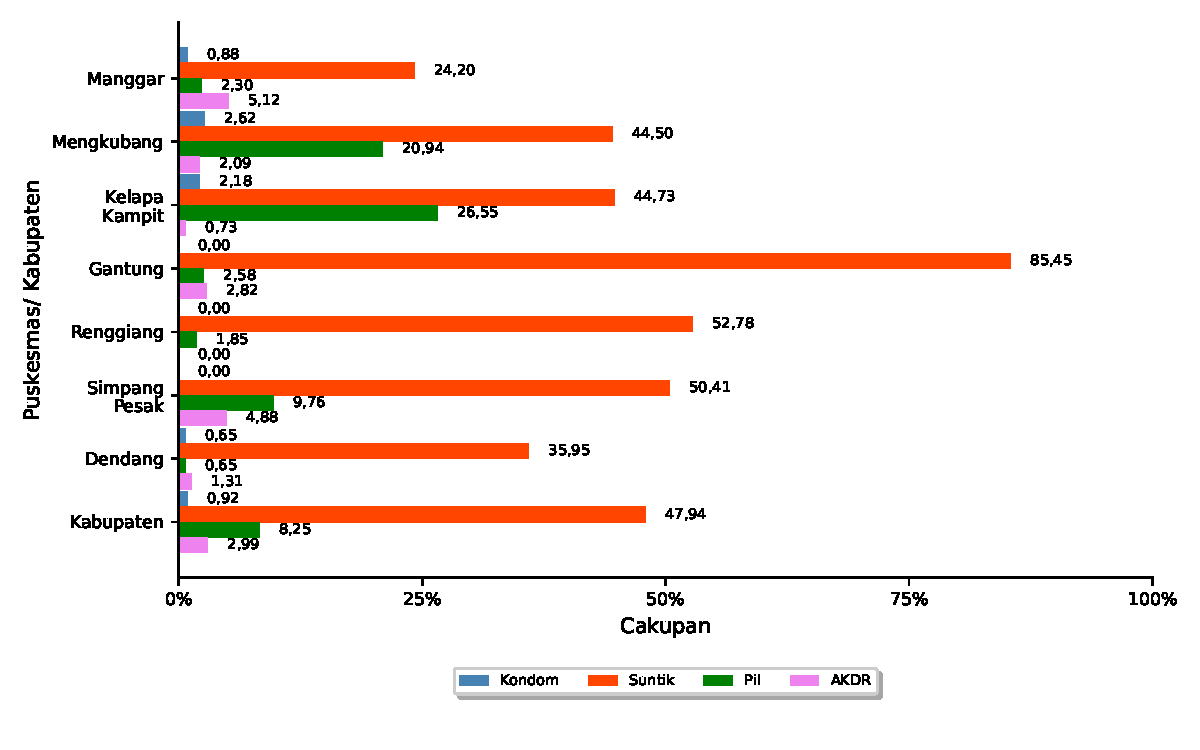
\includegraphics[width=0.85\textwidth]{bab_05/bab_05_07_KBpascaSalin_a}
    \caption{Cakupan Peserta KB Pasca Persalinan di Kab. Belitung Timur Tahun \tP per Puskesmas}
    \label{fig:Cakupan-KB-pascaSalin-a}
\end{figure}

\begin{figure}[!htb]
    \centering
    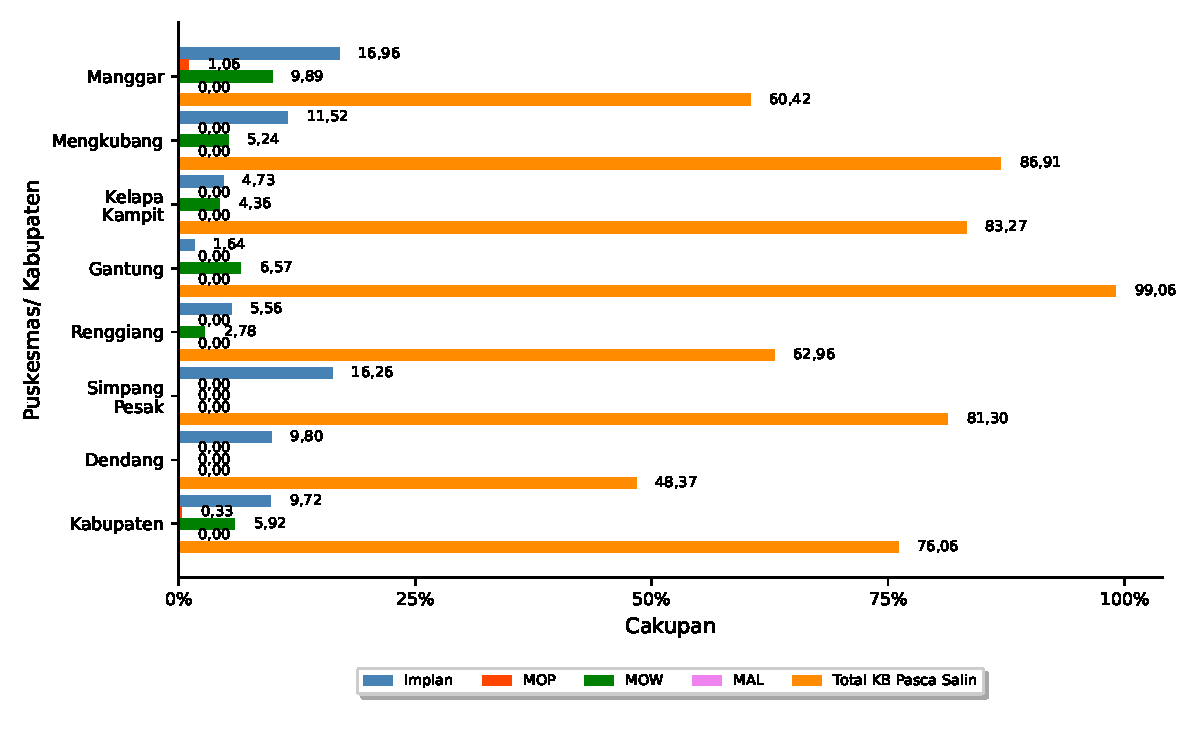
\includegraphics[width=0.85\textwidth]{bab_05/bab_05_07_KBpascaSalin_b}
    \caption{Cakupan Peserta KB Pasca Persalinan di Kab. Belitung Timur Tahun \tP per Puskesmas (lanj.)}
    \label{fig:Cakupan-KB-pascaSalin-b}
\end{figure}

\begin{figure}[H]
    \centering
    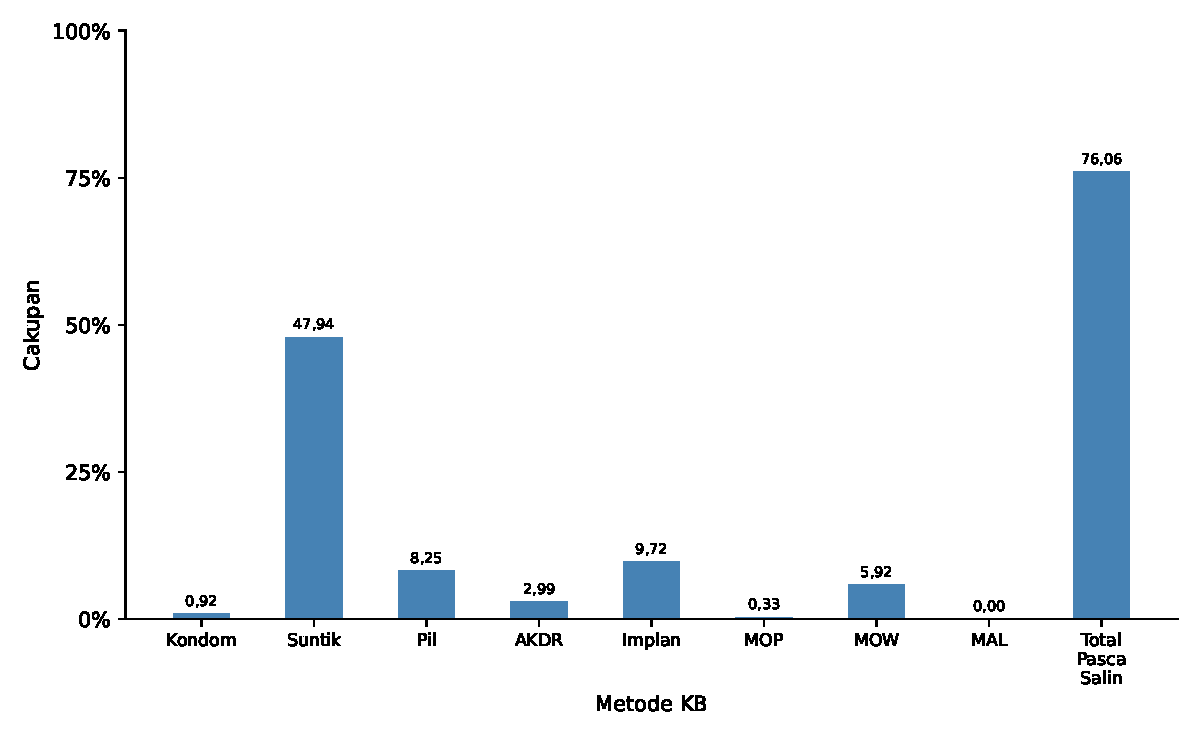
\includegraphics[width=0.9\textwidth]{bab_05/bab_05_07_KBpascaSalin_c}
    \caption{Cakupan Metode Yang Digunakan Peserta KB pasca Persalinan di Kab. Belitung Timur Tahun \tP}
    \label{fig:Cakupan-KB-pascaSalin-c}
\end{figure}

\section{KESEHATAN ANAK}
\subsection{Angka Kematian Neonatal (AKN)}
Kematian Neonatal adalah kematian yang terjadi pada bayi usia sampai dengan 28 hari tetapi bukan disebabkan oleh kecelakaan, bencana, cedera atau bunuh diri. Angka Kematian Neonatal per 1.000 kelahiran hidup adalah jumlah bayi usia sampai dengan 28 hari yang meninggal di suatu wilayah pada kurun waktu tertentu per 1.000 jumlah kelahiran hidup di wilayah dan pada kurun waktu yang sama.

Jumlah Kematian Neonatus yang terjadi di Kabupaten Belitung Timur sepanjang tahun \tP berjumlah 11 kematian (\autoref{fig:Jumlah-Kematian-Neonatal}). Angka Kematian Neonatal (AKN) pada tahun \tP sebesar 6,61 per 1.000 kelahiran hidup.

\begin{figure}[H]
    \centering{}
    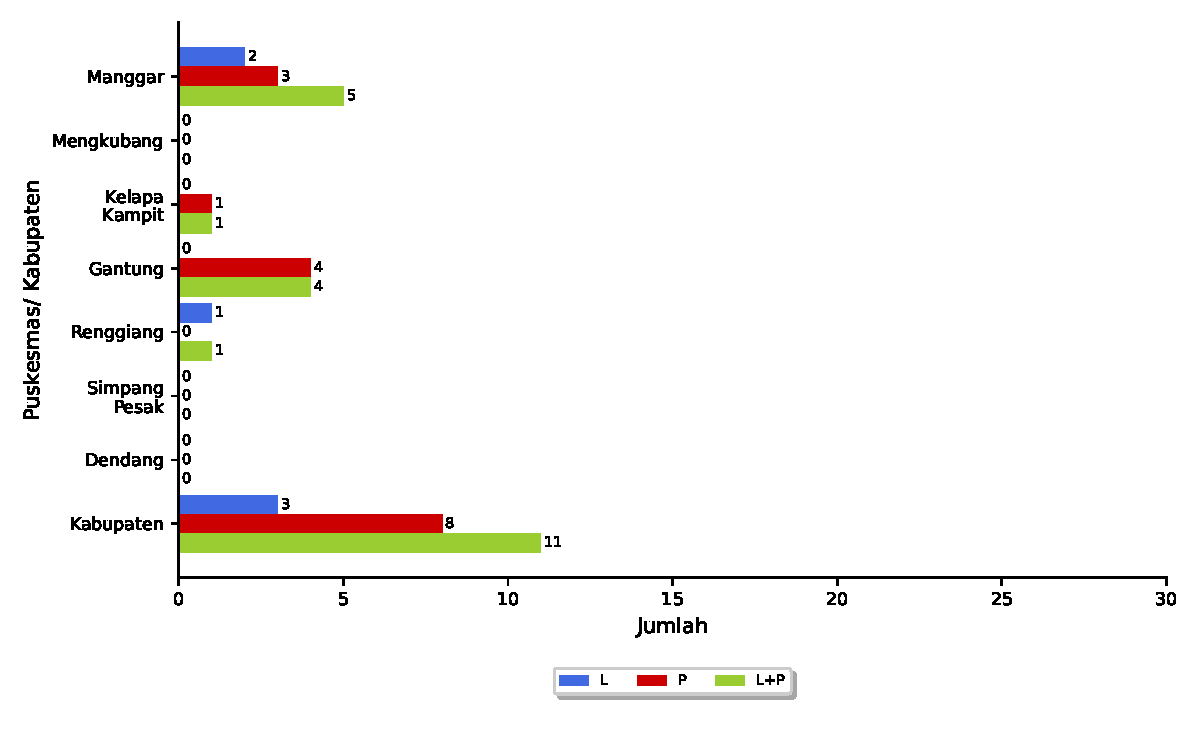
\includegraphics[width=0.85\textwidth]{bab_05/bab_05_09_kematianNeonatal}
    \caption{Jumlah Kematian Neonatal di Kab. Belitung Timur Tahun \tP per Puskesmas}
    \label{fig:Jumlah-Kematian-Neonatal}
\end{figure}

\begin{figure}[H]
    \centering{}
    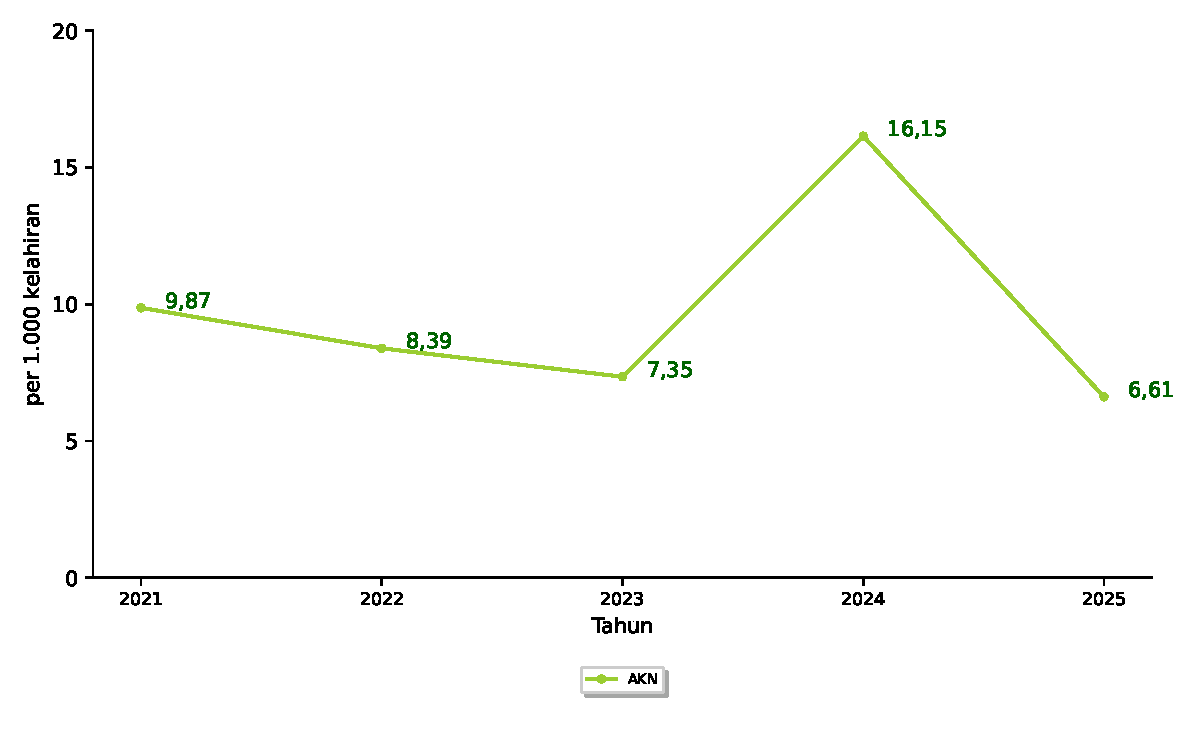
\includegraphics[width=0.85\textwidth]{bab_05/bab_05_09_plotNeonatal}
    \caption{AKN Kab. Belitung Timur Tahun \tPlot}
    \label{fig:AKN-\tPlotFig}
\end{figure}


\subsection{Angka Kematian Bayi (AKB)}
Kematian Bayi adalah kematian yang terjadi pada seorang bayi yang usianya sebelum mencapai satu tahun (usia 0-11 bulan, mencakup neonatal dan postnatal) tetapi bukan disebabkan oleh kecelakaan, bencana, cedera atau bunuh diri. Angka Kematian Bayi per 1.000 kelahiran hidup adalah jumlah bayi usia sampai dengan 11 bulan yang meninggal di suatu wilayah pada kurun waktu tertentu per 1.000 jumlah kelahiran hidup di wilayah dan pada kurun waktu yang sama.

Jumlah Kematian Bayi yang terjadi di Kabupaten Belitung Timur sepanjang tahun \tP berjumlah 18 kematian (\autoref{fig:Jumlah-Kematian-Bayi}). Angka Kematian Bayi (AKB) pada tahun \tP adalah sebesar 10,82 per 1.000 kelahiran hidup.

\begin{figure}[H]
    \centering{}
    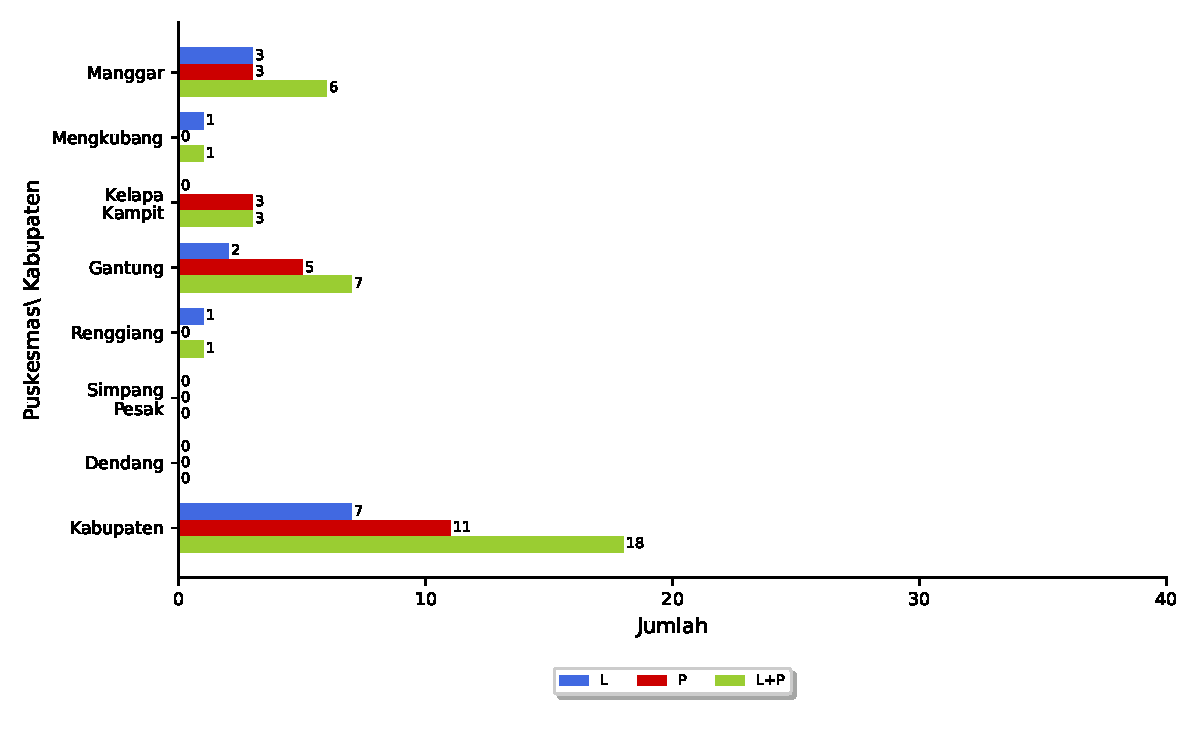
\includegraphics[width=0.85\textwidth]{bab_05/bab_05_10_kematianBayi}
    \caption{Jumlah Kematian Bayi di Kab. Belitung Timur Tahun \tP per Puskesmas}
    \label{fig:Jumlah-Kematian-Bayi}
\end{figure}

\begin{figure}[H]
    \centering{}
    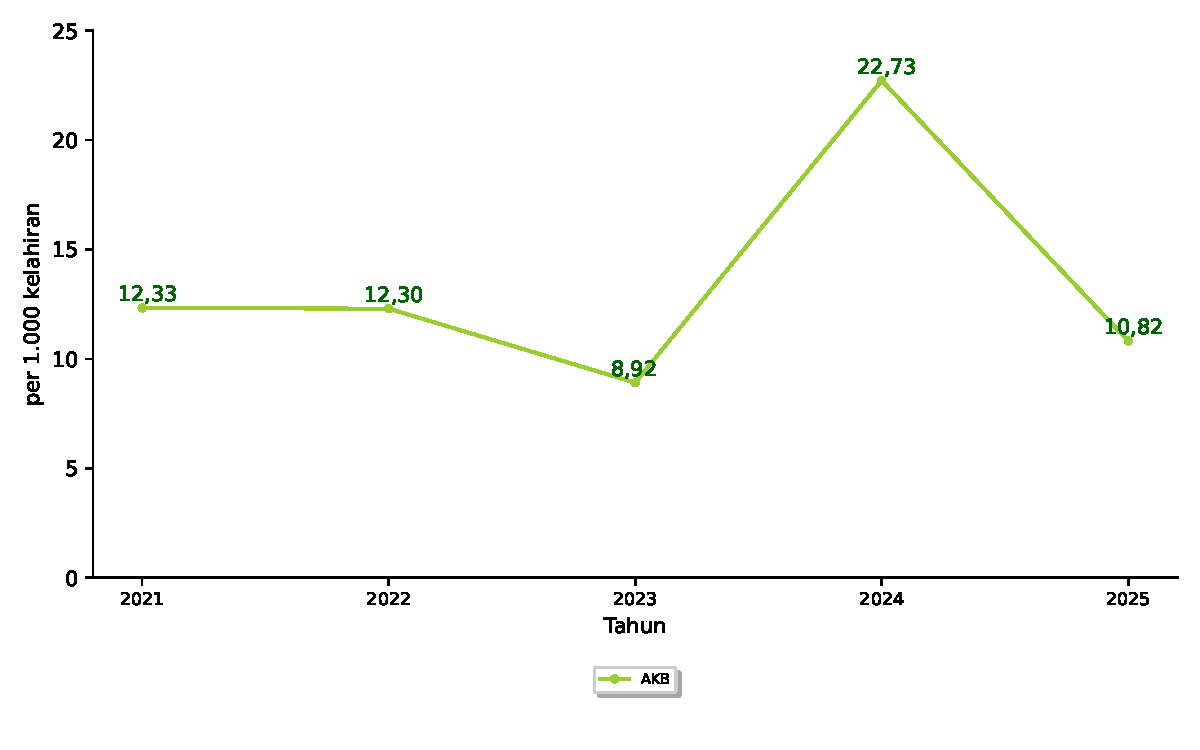
\includegraphics[width=0.85\textwidth]{bab_05/bab_05_10_plotBayi}
    \caption{AKB Kab. Belitung Timur Tahun \tPlot}
    \label{fig:AKB-\tPlotFig}
\end{figure}


\subsection{Angka Kematian Balita (AKBA)}
Kematian Balita adalah kematian yang terjadi pada bayi/anak usia 0 - 59 bulan (bayi + anak balita) tetapi bukan disebabkan oleh kecelakaan, bencana, cedera atau bunuh diri. Angka Kematian Balita (AKBA) adalah jumlah balita usia 59 bulan (mencakup bayi dan anak balita) yang meninggal di suatu wilayah pada kurun waktu tertentu
per 1.000 jumlah kelahiran hidup di wilayah pada kurun waktu yang sama.

Jumlah Kematian Balita yang terjadi di Kabupaten Belitung Timur sepanjang tahun \tP berjumlah 21 kematian (\autoref{fig:Jumlah-Kematian-Balita}). Angka Kematian Balita (AKBA) pada tahun \tP sebesar 12,63 per 1.000 kelahiran hidup.

\begin{figure}[H]
    \centering{}
    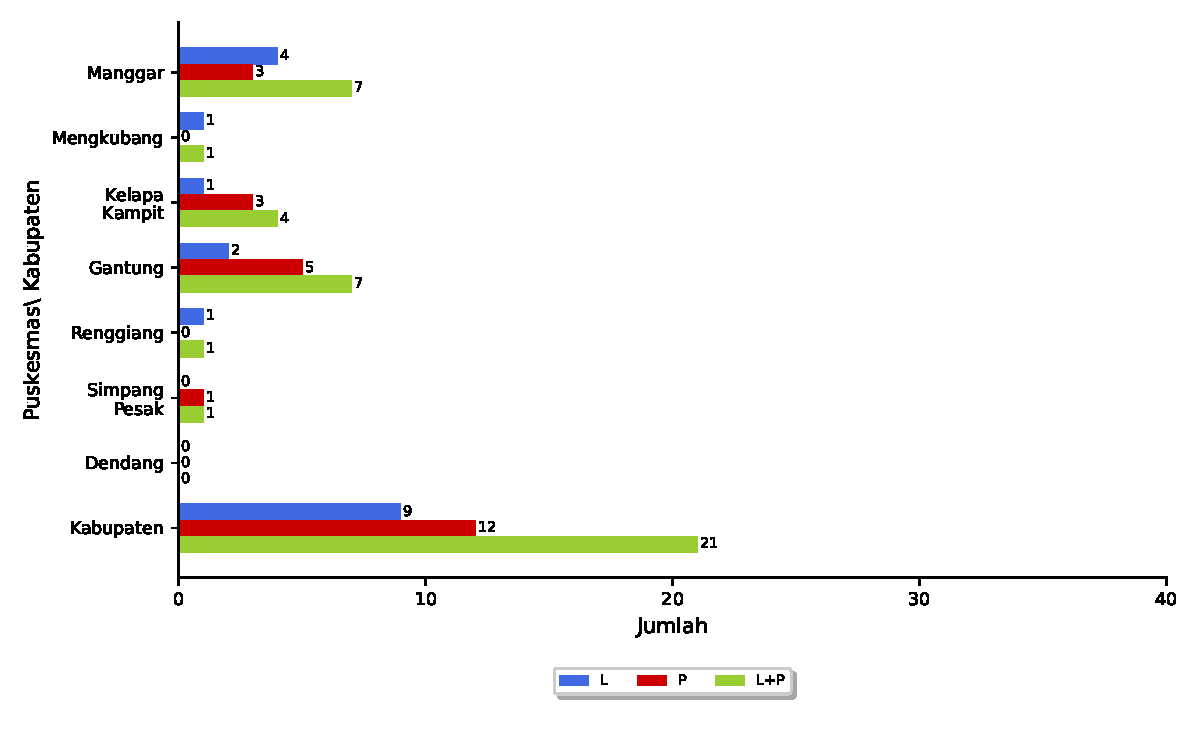
\includegraphics[width=0.85\textwidth]{bab_05/bab_05_11_kematianBalita}
    \caption{Jumlah Kematian Balita di Kabupaten Belitung Timur Tahun \tP per Puskesmas}
    \label{fig:Jumlah-Kematian-Balita}
\end{figure}

\begin{figure}[H]
    \centering{}
    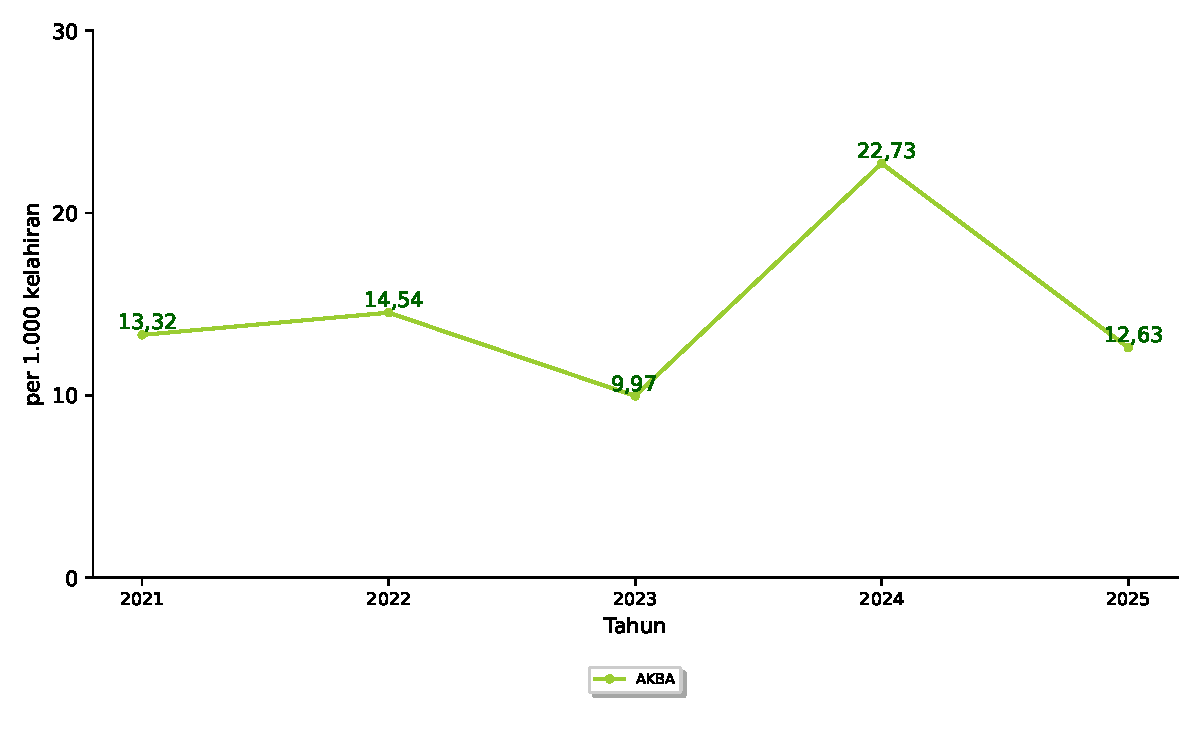
\includegraphics[width=0.8\textwidth]{bab_05/bab_05_11_plotBalita}
    \caption{AKABA Kabupaten Belitung Timur \tPlot}
    \label{fig:AKBA-\tPlotFig}
\end{figure}

\begin{figure}[H]
    \centering{}
    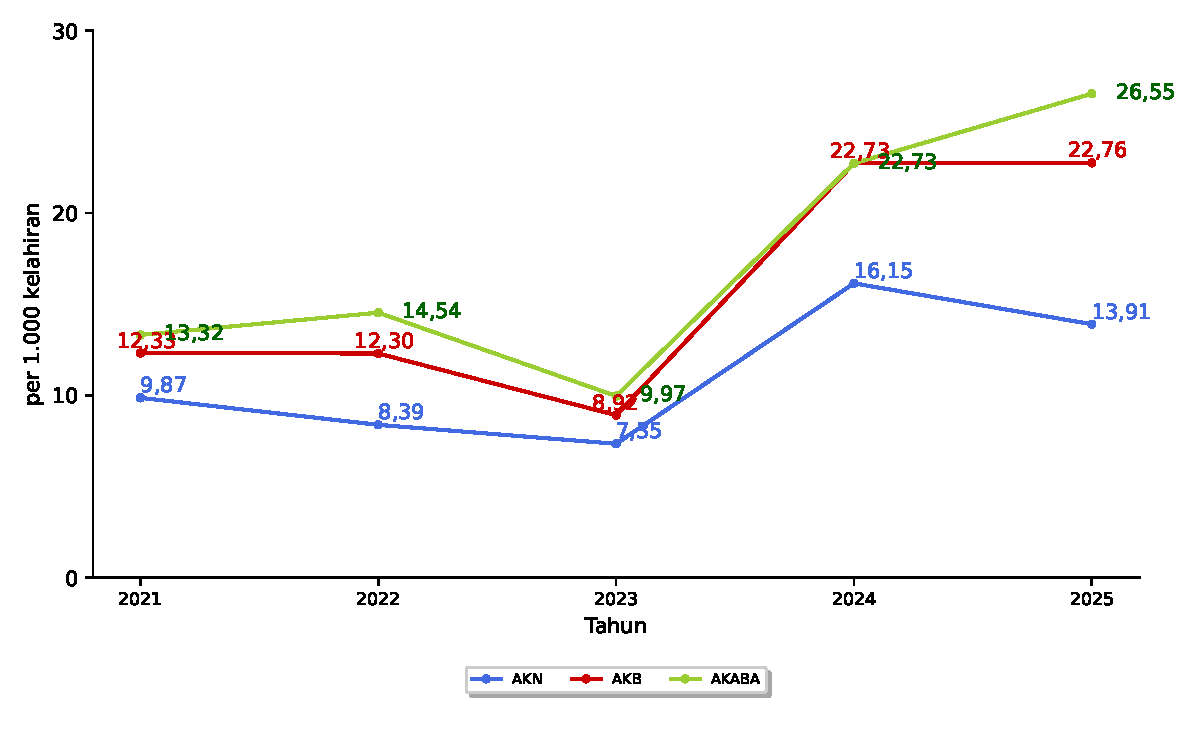
\includegraphics[width=0.8\textwidth]{bab_05/bab_05_11a_plotNeoBayiBalita}
    \caption{AKN, AKB dan AKBA Kabupaten Belitung Timur \tPlot}
    \label{fig:AKN-AKB-AKBA-\tPlotFig}
\end{figure}

\subsection{Penanganan Komplikasi Neonatal}
Komplikasi neonatal adalah neonatal dengan penyakit dan kelainan yang
dapat menyebabkan kesakitan, kecacatan, dan kematian neonatus dengan
komplikasi seperti BBLR (berat badan lahir rendah < 2500 gr), asfiksia, infeksi, tetanus neonatorum, kelainan kongenital, Covid 19, dan lain-lain
seperti ikterus, hipotermia, trauma lahir, sindroma gangguan pernafasan. Penanganan neonatal dengan komplikasi adalah
penanganan terhadap neonatal sakit dan atau neonatal dengan kelainan
atau komplikasi/kegawatdaruratan yang mendapat pelayanan sesuai standar
oleh tenaga kesehatan terlatih di seluruh sarana pelayanan kesehatan.
Pelayanan sesuai standar antara lain sesuai dengan standar MTBM, Manajemen
Asfiksia Bayi Baru Lahir, Manajemen Bayi Berat Lahir Rendah, pedoman
pelayanan neonatal essensial di tingkat pelayanan kesehatan dasar,
PONED, PONEK atau standar operasional pelayanan lainnya.

Persentase komplikasi neonatal di Kabupaten Belitung Timur pada tahun \tP adalah sebesar 10,82\%.
%menurun dari cakupan tahun2020 sebesar 78,26\% (\autoref{fig:Pelayanan-Komplikasi-Neonatal}).

\begin{figure}[H]
    \centering
    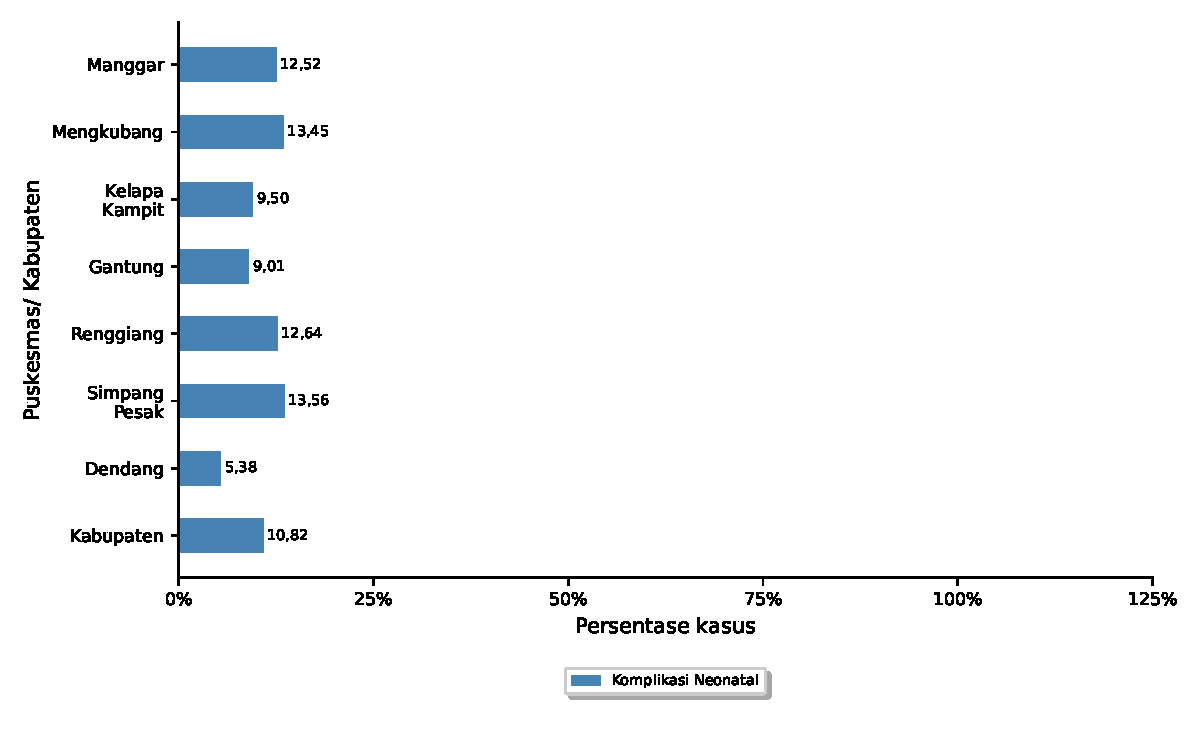
\includegraphics[width=0.85\textwidth]{bab_05/bab_05_12_komplikasiNeonatal}
    \caption{Persentase Komplikasi Neonatal di Kab. Belitung Timur Tahun \tP per Puskesmas}
    \label{fig:Pelayanan-Komplikasi-Neonatal}
\end{figure}


\subsection{Berat Badan Bayi Lahir Rendah (BBLR) dan Bayi Prematur}
Berat Badan Bayi Lahir Rendah adalah berat badan bayi kurang dari
2500 gram. BBLR dibedakan menjadi 2 (dua) kategori yaitu BBLR karena
prematur (kurang dari 37 minggu) dan BBLR karena \emph{Intrauterine Growth Restriction}(IUGR), yaitu bayi yang lahir cukup bulan tetapi berat badannya kurang.

Pada tahun \tP, tercatat bahwa Berat Badan Bayi Lahir Rendah adalah berjumlah
169 kasus atau 10,16\% dari jumlah kelahiran hidup (\autoref{fig:Distribusi-BBLR}).
%menurun dari cakupan tahun 2021 sebesar 5,53\%.

\begin{figure}[H]
  \centering
  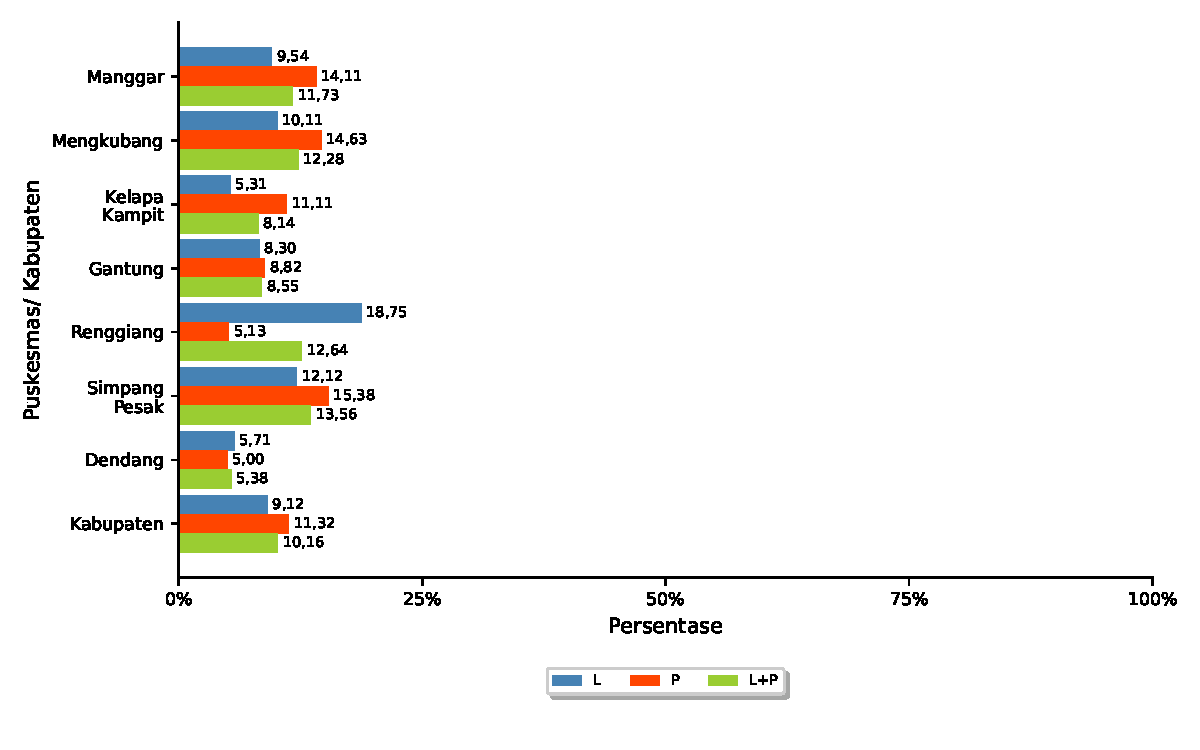
\includegraphics[width=0.85\textwidth]{bab_05/bab_05_13_BBLR}
  \caption{Sebaran BBLR di Kab. Belitung Timur Tahun \tP per Puskesmas}
  \label{fig:Distribusi-BBLR}
\end{figure}

Pada tahun \tP, tercatat bahwa Bayi Lahir Prematur adalah berjumlah
92 kasus atau 5,53\% dari jumlah kelahiran hidup (\autoref{fig:Distribusi-Prematur}).

\begin{figure}[H]
	\centering
	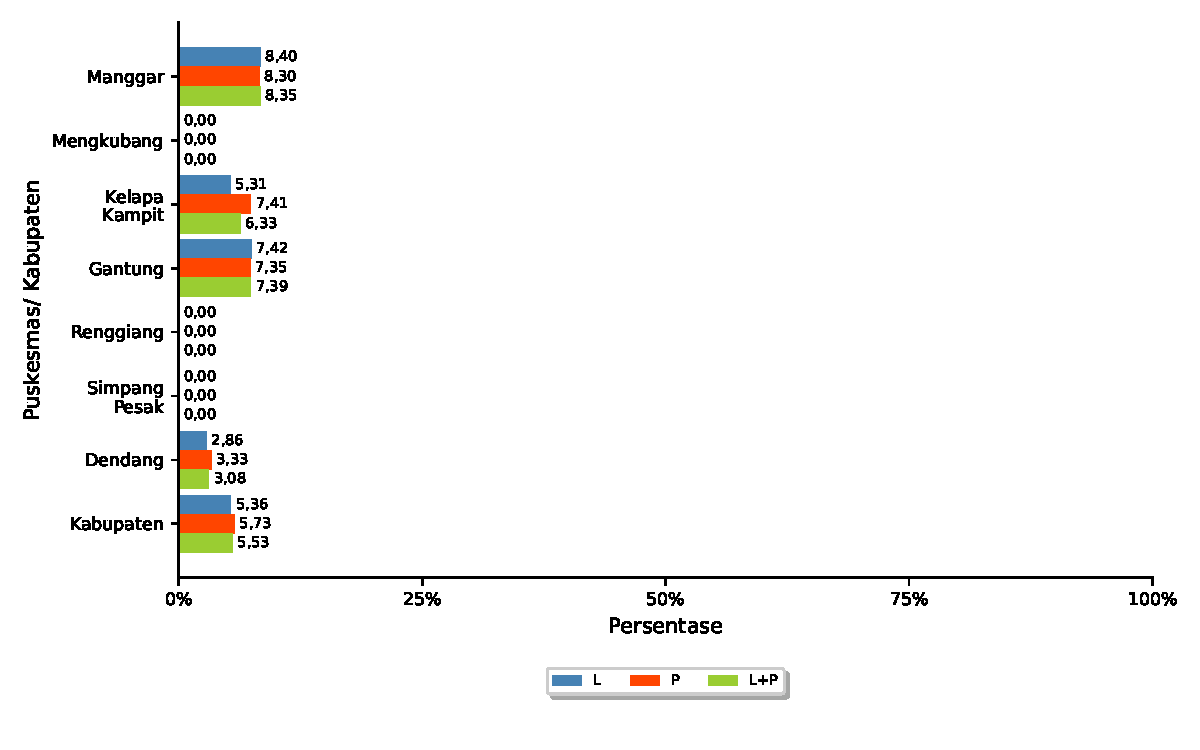
\includegraphics[width=0.85\textwidth]{bab_05/bab_05_13a_Prematur}
	\caption{Sebaran Bayi Lahir Prematur di Kab. Belitung Timur Tahun \tP per Puskesmas}
	\label{fig:Distribusi-Prematur}
\end{figure}

\subsection{Pelayanan Kesehatan Neonatal}
Neonatus adalah bayi baru lahir yang berusia sampai dengan 28 hari.
Pada masa tersebut terjadi perubahan yang sangat besar dari kehidupan
di dalam rahim dan terjadi pematangan organ hampir pada semua sistem.
Beberapa upaya kesehatan dilakukan untuk mengendalikan risiko pada
kelompok ini di antaranya dengan mengupayakan agar persalinan dapat
dilakukan oleh tenaga kesehatan di fasilitas kesehatan serta menjamin
tersedianya pelayanan kesehatan sesuai standar pada kunjungan bayi
baru lahir.

Indikator yang menggambarkan upaya kesehatan yang dilakukan untuk
mengurangi risiko kematian pada periode neonatal yaitu cakupan KN1
dan KN Lengkap. KN1 adalah pelayanan kunjungan neonatal pertama pada
6-48 jam setelah lahir sesuai standar di satu wilayah kerja. KN Lengkap
yaitu pelayanan kunjungan neonatal lengkap, minimal 3 kali yaitu 1
kali pada usia 6 - 48 jam, 1 kali pada 3 - 7 hari, dan 1 kali pada
8 - 28 hari sesuai standar.

%Cakupan penanganan KN1 di Kabupaten Belitung Timur
%pada tahun \tP sebesar 100,00\%, meningkat
%dari cakupan tahun 2019 sebesar 99,90\%. Sedangkan cakupan penanganan KN Lengkap di Kabupaten Belitung Timur
%pada tahun \tP 98,67\%, menurun
%dari cakupan tahun 2019 sebesar 99,60\% (\autoref{fig:Cakupan-KN1-KNlengkap} dan \autoref{fig:KN1-KNlengkap-2016-2020}).

Cakupan penanganan KN1 di Kabupaten Belitung Timur pada tahun \tP sebesar 99,76\%.
Sedangkan cakupan penanganan KN Lengkap di Kabupaten Belitung Timur pada tahun \tP sebesar 98,92\% (\autoref{fig:Cakupan-KN1-KNlengkap}

% dan \autoref{fig:KN1-KNlengkap-2016-2020}).

\begin{figure}[H]
    \centering
    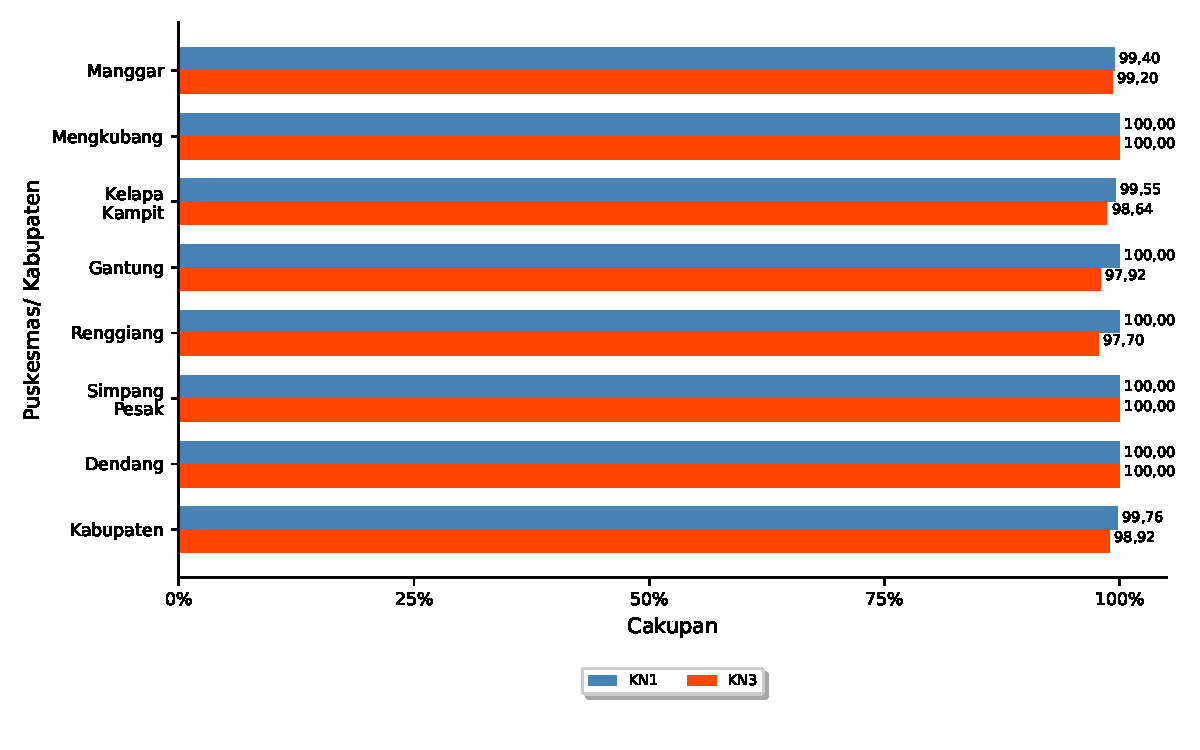
\includegraphics[width=0.9\textwidth]{bab_05/bab_05_14_KN1KN3}
    \caption{Cakupan KN1 dan KN Lengkap di Kabupaten Belitung Timur tahun \tP per Puskesmas}
    \label{fig:Cakupan-KN1-KNlengkap}
\end{figure}

%\begin{figure}[H]
%    \centering
%%%    \includegraphics[width=0.9\textwidth]{bab_05/bab_05_14a_plotKN1KN3}
%    \caption{Cakupan KN1 dan KN Lengkap di Kab. Belitung Timur Tahun 2017-2021}
%    \label{fig:KN1-KNlengkap-2016-2020}
%\end{figure}

Hipotiroid Kongenital adalah gangguan defisiensi hormon tiroid yang timbul pada bayi baru lahir yang dapat menimbulkan gangguan tumbuh kembang pada bayi.
Skrining Hipotiroid Kongenital (SHK) dilakukan dengan mengambil spesimen darah pada tumit bayi baru lahir berusia minimal 48 sampai 72 jam dan maksimal 2 minggu.

Cakupan SHK di Kabupaten Belitung Timur pada tahun \tP adalah sebesar 95,01\%.

\begin{figure}[H]
	\centering
	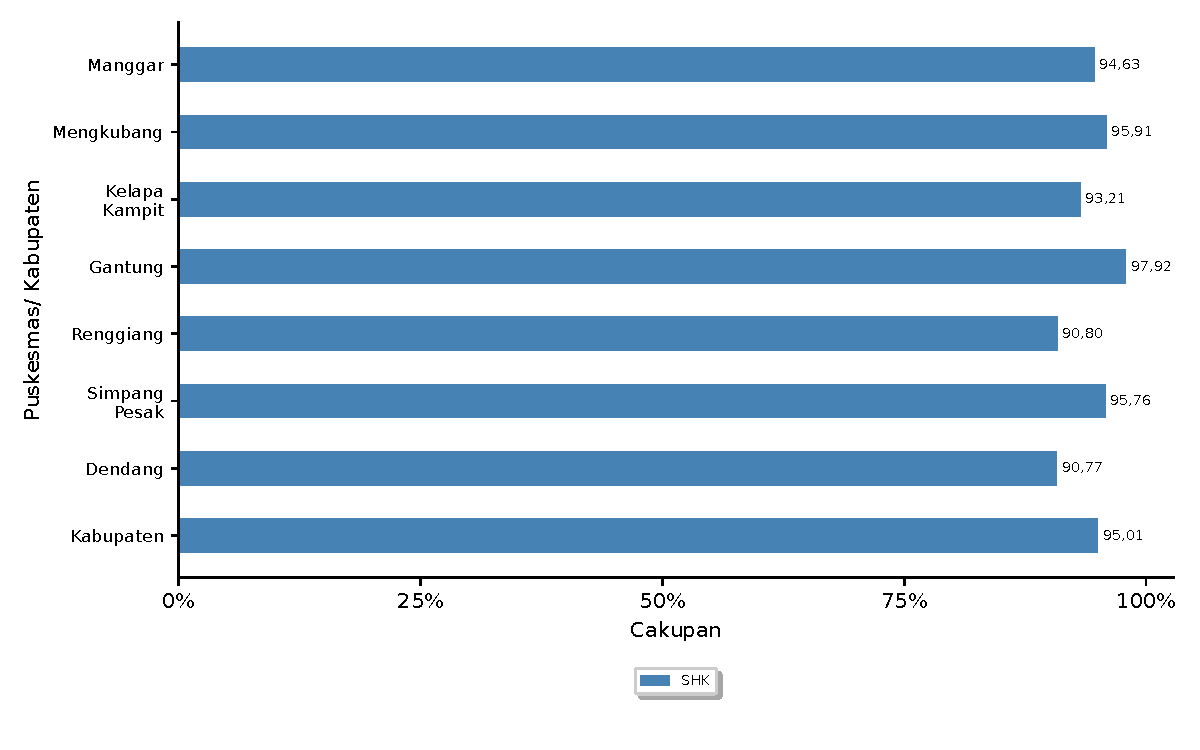
\includegraphics[width=0.9\textwidth]{bab_05/bab_05_14c_SHK}
	\caption{Cakupan SHK di Kabupaten Belitung Timur tahun \tP per Puskesmas}
	\label{fig:Cakupan-SHK}
\end{figure}

\subsection{Bayi Mendapat ASI Eksklusif}
Air Susu Ibu (ASI) adalah cairan hasil sekresi kelenjar payudara ibu
untuk konsumsi bayi dan merupakan sumber gizi utama bayi yang belum
dapat mencerna makanan padat. ASI eksklusif berdasarkan Peraturan
Pemerintah Nomor 33 Tahun 2012 adalah ASI yang diberikan kepada bayi
sejak dilahirkan selama enam bulan, tanpa menambahkan dan/atau mengganti
dengan makanan atau minuman lain (kecuali obat, vitamin, dan mineral).

Cakupan bayi mendapat ASI eksklusif di kabupaten Belitung Timur pada
tahun \tP yaitu sebesar 75,20\% (\autoref{fig:Cakupan-Bayi-ASI-Eksklusif}).
% meningkat dari cakupan tahun 2021 sebesar 45,62\%.

\begin{figure}[H]
  \centering
  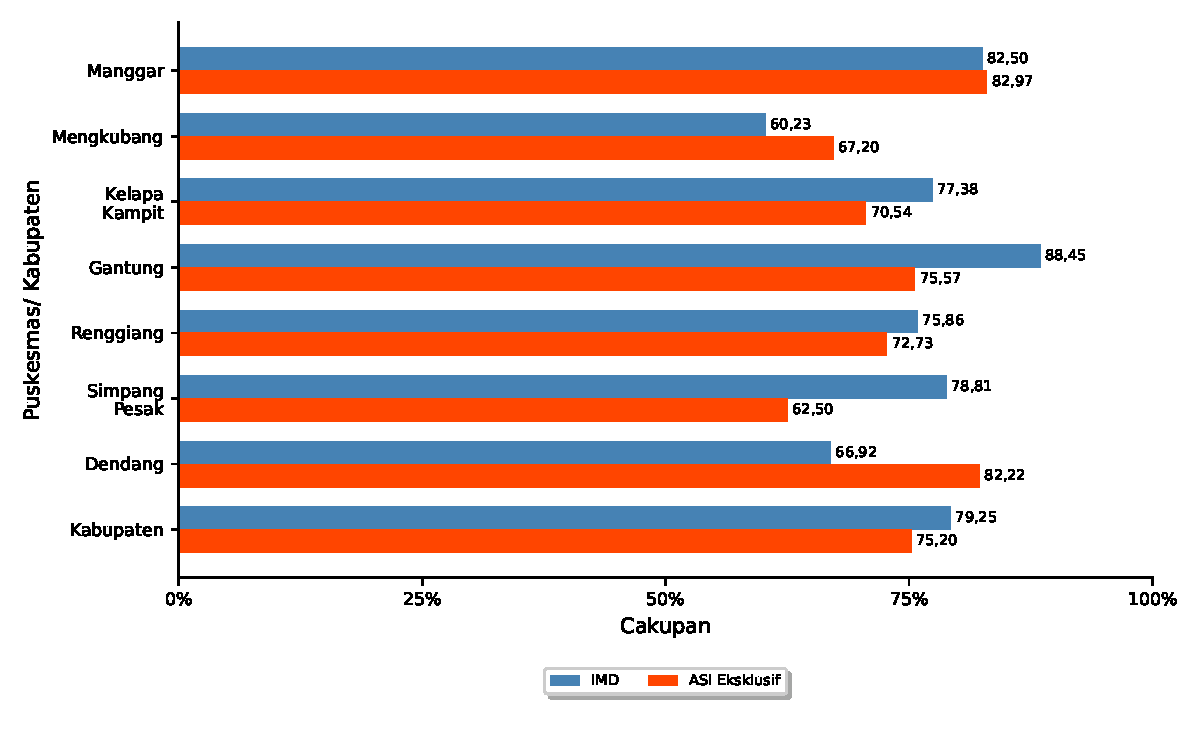
\includegraphics[width=0.9\textwidth]{bab_05/bab_05_15_ASIeksklusif}
  \caption{Cakupan Bayi Mendapat ASI Eksklusif di Kab. Belitung Timur Tahun \tP per Puskesmas}
  \label{fig:Cakupan-Bayi-ASI-Eksklusif}
\end{figure}

%\subsection{Pelayanan Kesehatan Bayi}
%Pelayanan kesehatan bayi adalah pelayanan kesehatan pada bayi minimal
%4 kali yaitu satu kali pada umur 29 hari-2 bulan, 1 kali pada umur
%3-5 bulan, 1 kali pada umur 6-8 bulan, dan 1 kali pada umur 9-11 bulan.
%Pelayanan Kesehatan tersebut meliputi pemberian imunisasi dasar (BCG,
%DPT/HB1-3, Polio 1-4, Campak), pemantauan pertumbuhan, Stimulasi Deteksi
%Intervensi Dini Tumbuh Kembang (SDIDTK), pemberian vitamin A pada
%bayi umur 6-11 bulan, penyuluhan pemberian ASI eksklusif dan Makanan
%Pendamping ASI (MP ASI).
%
%Cakupan pelayanan kesehatan bayi di Kabupaten Belitung Timur pada
%tahun \tP adalah sebesar 81,37\% (~\autoref{fig:Cakupan-Pelayanan-Kesehatan-Bayi}).
%% meningkat dari cakupan tahun 2020 sebesar 94,11\%.
%
%\begin{figure}[H]
%    \centering
%%    \includegraphics[width=0.85\textwidth]{bab_05/bab_05_16_pelayananBayi}
%    \caption{Cakupan Pelayanan Kesehatan Bayi di Kab. Belitung Timur tahun \tP per Puskesmas}
%    \label{fig:Cakupan-Pelayanan-Kesehatan-Bayi}
%\end{figure}

%\subsection{Cakupan Desa/ Kelurahan UCI}
%Pencapaian \emph{Universal Child Immunization} (UCI) pada dasarnya merupakan
%\emph{proxy} terhadap cakupan sasaran bayi yang telah mendapatkan imunisasi
%secara lengkap. Desa/ kelurahan UCI adalah Desa/ kelurahan dimana
%paling sedikit 80\% dari jumlah bayi yang ada di desa tersebut sudah
%mendapat imunisasi dasar lengkap dalam waktu satu tahun.
%
%Pada tahun \tP sebanyak 29 desa dari total 39 desa yang ada di Kabupaten Belitung
%Timur telah mencapai UCI, sehingga capaian UCI Kabupaten Belitung
%Timur pada tahun \tP adalah 74,36\% (\autoref{fig:Cakupan-Desa-UCI}).
%
%\begin{figure}[H]
%    \centering
%%    \includegraphics[width=0.85\textwidth]{bab_05/bab_05_17_UCI}
%    \caption{Cakupan Desa/ Kelurahan UCI di Kab. Belitung Timur Tahun \tP per Puskesmas}
%    \label{fig:Cakupan-Desa-UCI}
%\end{figure}

\subsection{Imunisasi}
Imunisasi adalah upaya stimulasi terhadap sistem kekebalan tubuh untuk
menghasilkan antibodi dalam upaya melawan penyakit menular tertentu.
Program imunisasi melalui pemberian vaksin merangsang antibodi menggunakan
antigen yang telah dilemahkan yang berasal dari vaksin. Beberapa penyakit
menular yang termasuk ke dalam Penyakit yang Dapat Dicegah dengan
Imunisasi (PD3I) antara lain TBC, Difteri, Tetanus, Hepatitis B, Pertusis,
Campak, Polio, radang selaput otak, dan radang paru-paru.

\subsubsection{Imunisasi pada bayi}
Imunisasi lengkap 14 antigen mencapai target adalah cakupan imunisasi HB0, BCG, DPT-HB-Hib 1, PCV 1, bOPV 1, Rotavirus 1, IPV 1, MR 1, JE (hanya di daerah tertentu), dan HPV 1 pada bayi.

Cakupan imunisasi 14 antigen mencapai target di Kabupaten Belitung Timur pada tahun \tP adalah sebesar 80,32\% (\autoref{fig:Cakupan-Imunisasi-14-antigen}).

\begin{figure}[H]
	\centering
	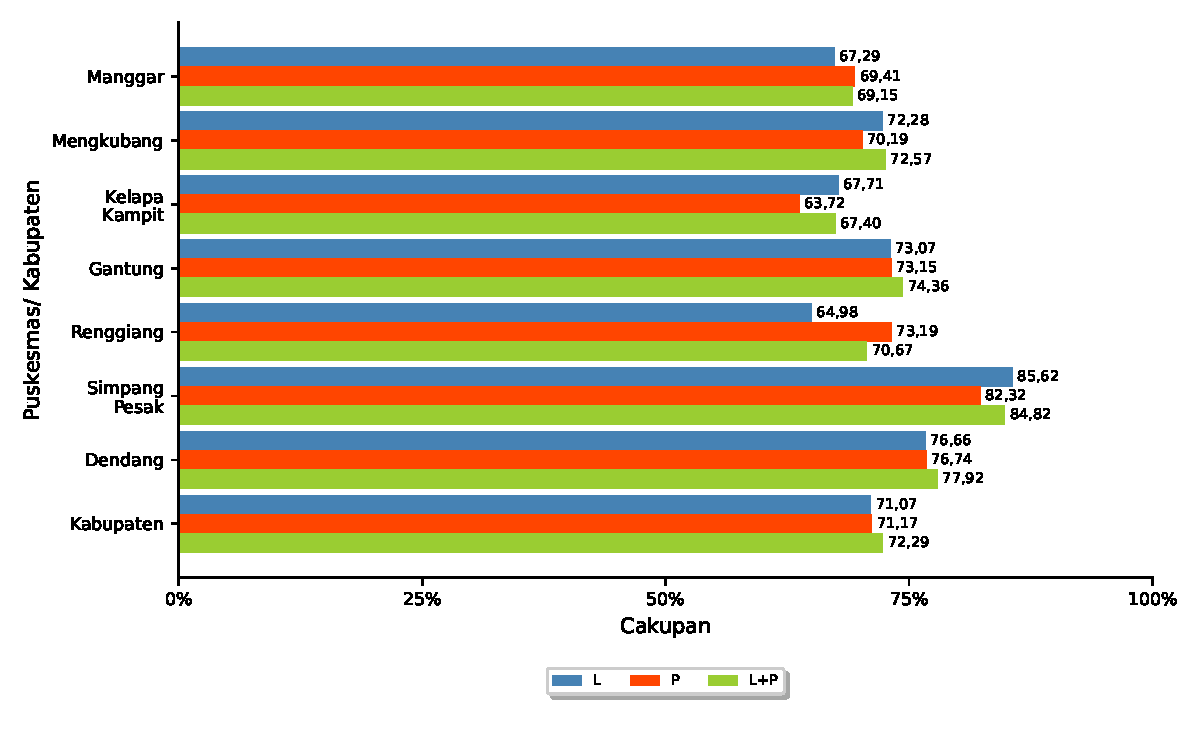
\includegraphics[width=0.85\textwidth]{bab_05/bab_05_18_dataImun14Antigen}
	\caption{Cakupan Imunisasi 14 Antigen di Kab. Belitung Timur Tahun \tP per Puskesmas}
	\label{fig:Cakupan-Imunisasi-14-antigen}
\end{figure}

Program imunisasi pada bayi bertujuan agar setiap bayi mendapatkan
imunisasi dasar secara lengkap. Bayi dikatakan mendapat imunisasi
dasar lengkap jika telah menerima 1 dosis imunisasi Hepatitis B pada
usia 0-7 hari, 1 dosis imunisasi BCG pada usia 0-11 bulan, 4 dosis imunisasi
Polio usia 0-11 bulan dengan interval minimal 1 bulan, 3 dosis imunisasi
DPT-HB/DPT-HB-Hib pada usia 2-11 bulan dengan interval minimal
1 bulan, dan 1 dosis imunisasi Campak pada usia 9-11 bulan.

Cakupan imunisasi bayi lengkap di Kabupaten Belitung Timur pada tahun \tP adalah sebesar 87,64\% (\autoref{fig:Cakupan-Imunisasi-IDL}).

\begin{figure}[H]
    \centering
    \includegraphics[width=0.85\textwidth]{bab_05/bab_05_19_imunBayiLengkap}
    \caption{Cakupan Imunisasi Bayi Lengkap di Kab. Belitung Timur Tahun \tP per Puskesmas}
    \label{fig:Cakupan-Imunisasi-IDL}
\end{figure}

Imunisasi antigen baru mencakup pemberian 2 dosis imunisasi PCV atau 3 dosis imunisasi rotavirus pada bayi usia 0-11 bulan.

Cakupan imunisasi antigen baru di Kabupaten Belitung Timur pada tahun \tP adalah sebesar 75,78\% (\autoref{fig:Cakupan-Imunisasi-IDL}).

\begin{figure}[H]
	\centering
	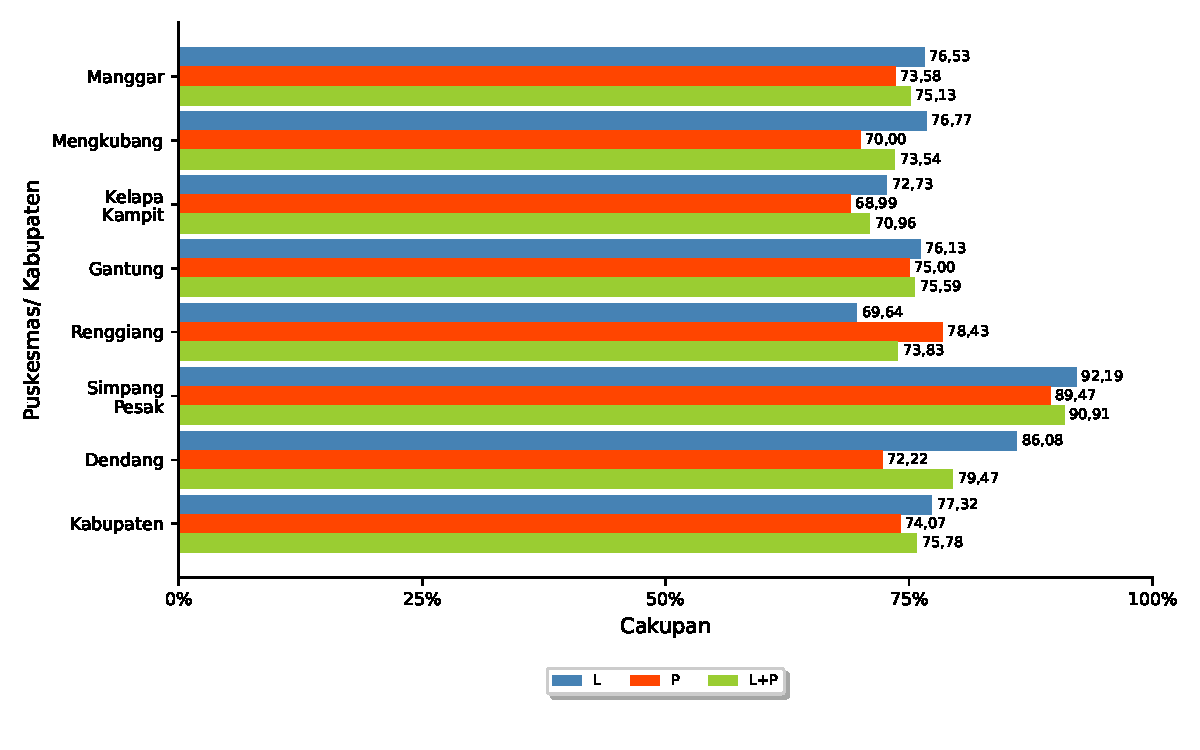
\includegraphics[width=0.85\textwidth]{bab_05/bab_05_20_imunAntigenBaru}
	\caption{Cakupan Imunisasi Antigen Baru di Kab. Belitung Timur Tahun \tP per Puskesmas}
	\label{fig:Cakupan-Imunisasi-antigen-baru}
\end{figure}

\subsubsection{Imunisasi pada balita}
Imunisasi lanjutan diperlukan untuk mempertahankan tingkat kekebalan yang optimal pada anak.
Imunisasi lanjutan meliputi pemberian imunisasi DPT-HB-Hib 4 pada anak usia 12-24 bulan serta imunisasi Campak 2 pada anak usia 12-24 bulan.

Cakupan imunisasi DPT-HB-Hib 4 di Kabupaten Belitung Timur pada tahun \tP
adalah sebesar 81,38\% (\autoref{fig:Cakupan-Imunisasi-DPT4}), sedangkan cakupan imunisasi Campak 2 adalah 80,37\% (\autoref{fig:Cakupan-Imunisasi-Campak2}).

\begin{figure}[H]
    \centering
    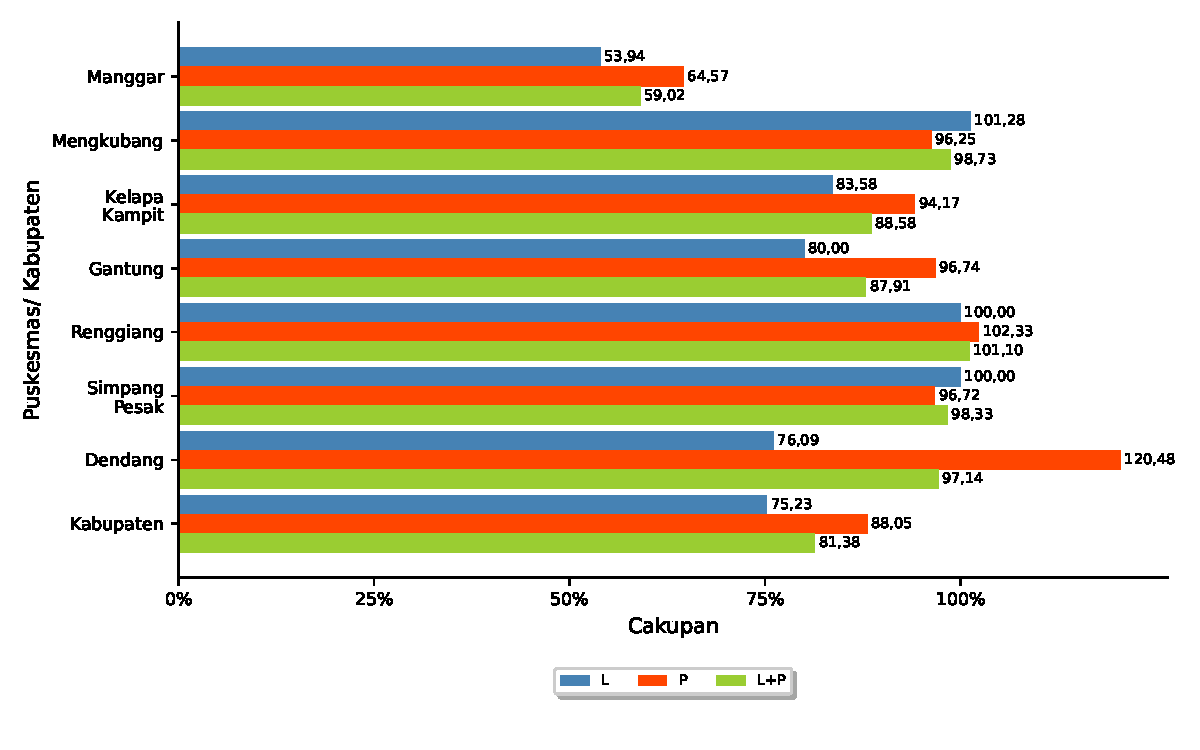
\includegraphics[width=0.85\textwidth]{bab_05/bab_05_21a_imunDPTlanjut}
    \caption{Cakupan Imunisasi DPT-HB-Hib 4 di Kab. Belitung Timur Tahun \tP per Puskesmas}
    \label{fig:Cakupan-Imunisasi-DPT4}
\end{figure}

\begin{figure}[H]
    \centering
    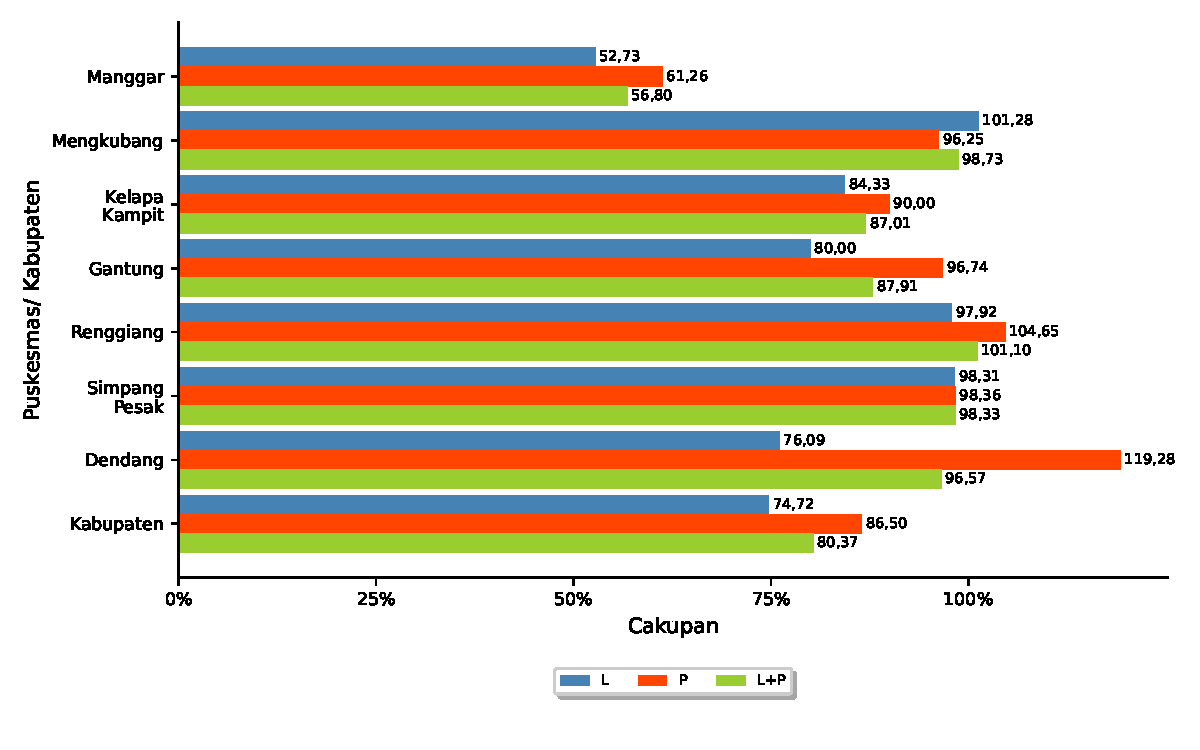
\includegraphics[width=0.85\textwidth]{bab_05/bab_05_21b_imunCampakLanjut}
    \caption{Cakupan Imunisasi Campak 2 di Kab. Belitung Timur Tahun \tP per Puskesmas}
    \label{fig:Cakupan-Imunisasi-Campak2}
\end{figure}

\subsection{Pemberian Kapsul Vitamin A}
Upaya perbaikan gizi juga dilakukan kepada beberapa sasaran yang diperkirakan
banyak mengalami kekurangan Vitamin A. Vitamin A adalah salah satu
zat gizi penting yang larut dalam lemak, disimpan dalam hati, dan
tidak dapat diproduksi oleh tubuh sehingga harus dipenuhi dari luar
tubuh. Kekurangan Vitamin A (KVA) dapat menurunkan sistem kekebalan
tubuh balita serta meningkatkan risiko kesakitan dan kematian. Kekurangan
Vitamin A juga merupakan penyebab utama kebutaan pada anak yang dapat
dicegah.

Pemberian Vitamin A dilakukan berupa pemberian kapsul vitamin A biru 100.000 IU bagi bayi
usia enam sampai dengan sebelas bulan, dan kapsul vitamin A merah 200.000
IU untuk anak balita usia dua belas sampai dengan lima puluh sembilan sebanyak
bulan.

Cakupan pemberian vitamin A pada balita usia 6-59 tahun pada tahun \tP di Kabupaten Belitung Timur adalah 99,08\% (\autoref{fig:Cakupan-Vitamin-A-Balita}).
% meningkat dari cakupan tahun 2021 sebesar 81,47\%.

\begin{figure}[H]
    \centering
    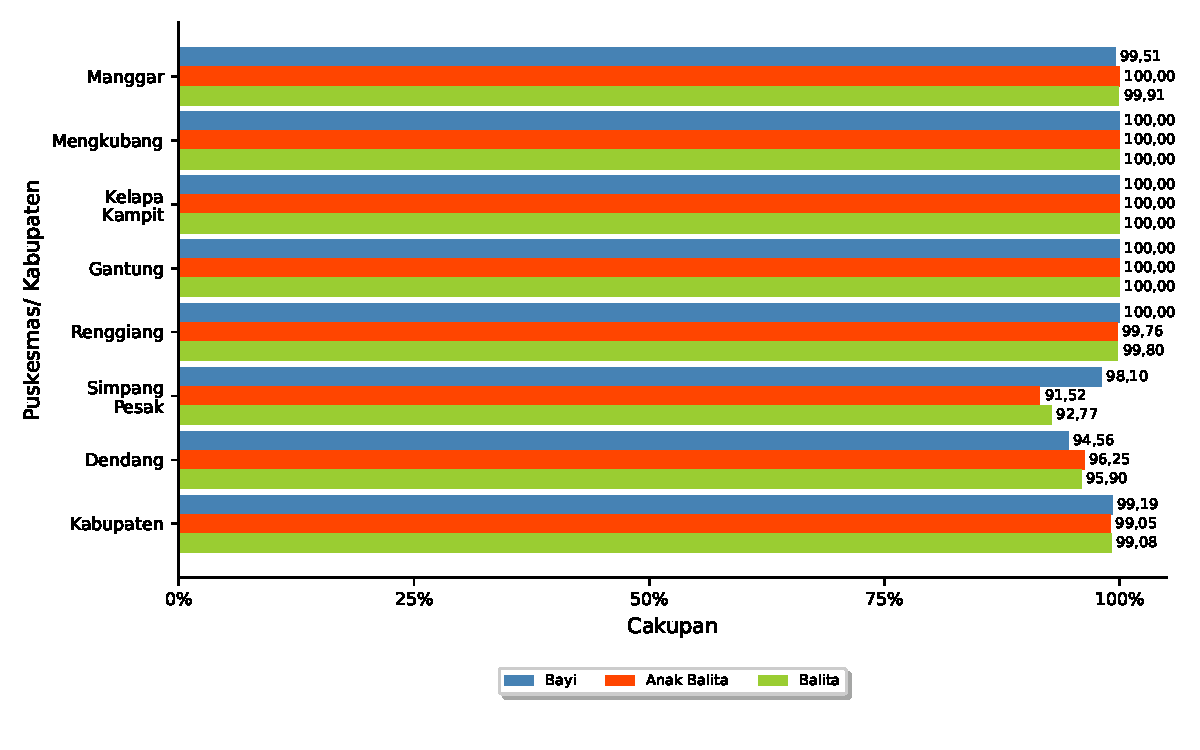
\includegraphics[width=0.9\textwidth]{bab_05/bab_05_22_bayiBalitaVitA}
    \caption{Cakupan Pemberian Vitamin A Balita 6-59 Bulan di Kab. Belitung Timur Tahun \tP per Puskesmas}
    \label{fig:Cakupan-Vitamin-A-Balita}
\end{figure}


\subsection{Pelayanan Kesehatan Anak Balita}
Pelayanan kesehatan anak balita mencakup pemantauan tumbuh kembang dan pelayanan Stimulasi Deteksi dan Intervensi Dini Tumbuh Kembang (SDIDTK).
Balita yang dipantau tumbuh kembang adalah  balita yang ditimbang sedikitnya 8 kali dalam satu tahun, diukur panjang badan atau tinggi badannya sedikitnya 2 kali dalam satu tahun dan dipantau perkembangan sedikitnya 2 kali dalam satutahun. Pemantauan perkembangan menggunakan ceklis Buku KIA atau KPSP atau instrument baku lainnya.
Balita dilayani SDIDTK adalah balita yang dipantau tahapan perkembangan sesuai usianya (usia 0-24 bulan: 3 bulan sekali; usia 24-72 bulan: 6 bulan sekali) menggunakan instrument dalam SDIDTK oleh tenaga kesehatan dalam kurun waktu 1 tahun.

Cakupan balita dipantau tumbuh kembang di Kabupaten Belitung Timur pada tahun \tP adalah sebesar 90,97\%, sedangkan cakupan balita dilayani SDIDTK di Kabupaten Belitung Timur pada tahun \tP adalah sebesar 56,25\%. (\autoref{fig:Cakupan-Pelayanan-Balita-Tumbuh-Kembang}).

\begin{figure}[H]
	\centering
	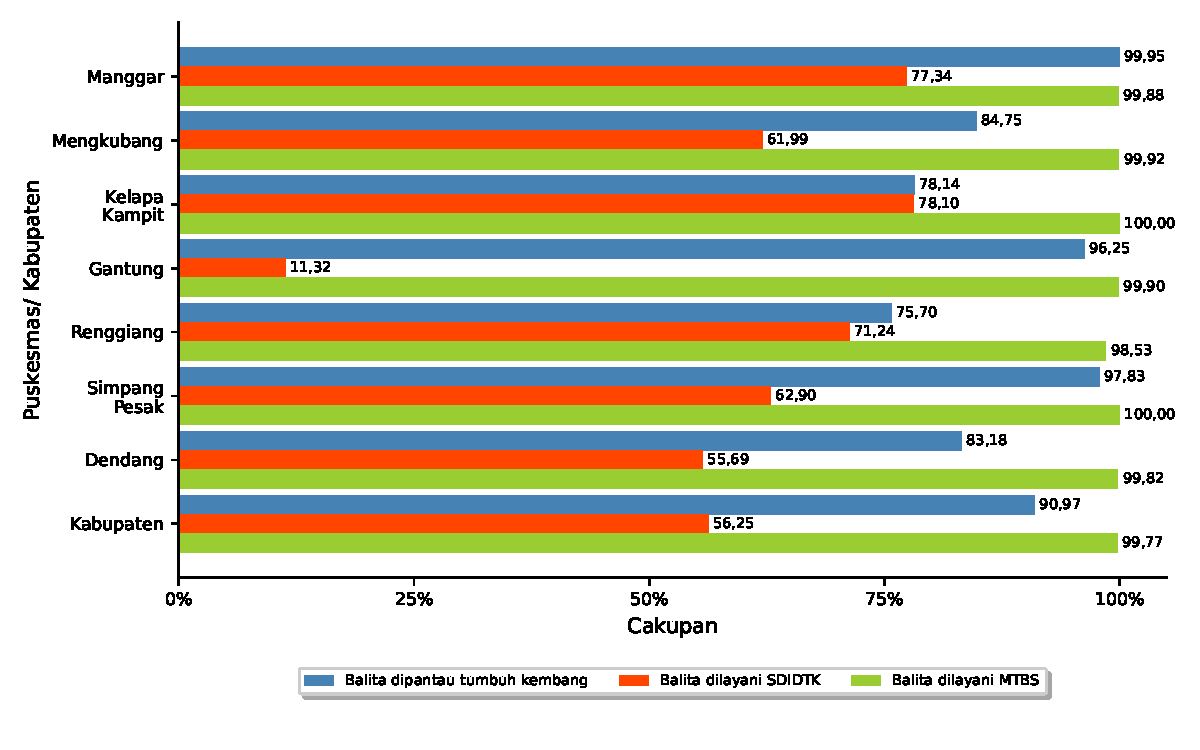
\includegraphics[width=0.85\textwidth]{bab_05/bab_05_23_balitaTumbuhKembang}
	\caption{Cakupan Balita Dipantau Tumbuh Kembang di Kab. Belitung Timur tahun \tP per Puskesmas}
	\label{fig:Cakupan-Pelayanan-Balita-Tumbuh-Kembang}
\end{figure}

\subsection{Balita Ditimbang}
\label{subsec:Balita-Ditimbang}
Peran serta masyarakat dalam penimbangan balita menjadi sangat penting
dalam deteksi dini kasus gizi kurang dan gizi buruk. Dengan rajin
menimbang balita, maka pertumbuhan balita dapat dipantau secara intensif.
Sehingga bila berat badan anak tidak naik ataupun jika ditemukan penyakit
akan dapat segera dilakukan upaya pemulihan dan pencegahan supaya
tidak menjadi gizi kurang atau gizi buruk. Semakin cepat ditemukan,
maka penanganan kasus gizi kurang atau gizi buruk akan semakin baik.\par

Cakupan penimbangan balita di posyandu (D/S) adalah jumlah balita
yang ditimbang di seluruh posyandu yang melapor di satu wilayah kerja
pada kurun waktu tertentu dibagi jumlah seluruh balita yang ada di
seluruh posyandu yang melapor di satu wilayah kerja pada kurun waktu
tertentu.

Cakupan balita ditimbang di Kabupaten Belitung Timur pada tahun \tP yaitu sebesar 78,18\% (\autoref{fig:Cakupan-Balita-Ditimbang}). %meningkat dari cakupan tahun 2020 sebesar 57,91\%.

\begin{figure}[H]
  \centering
  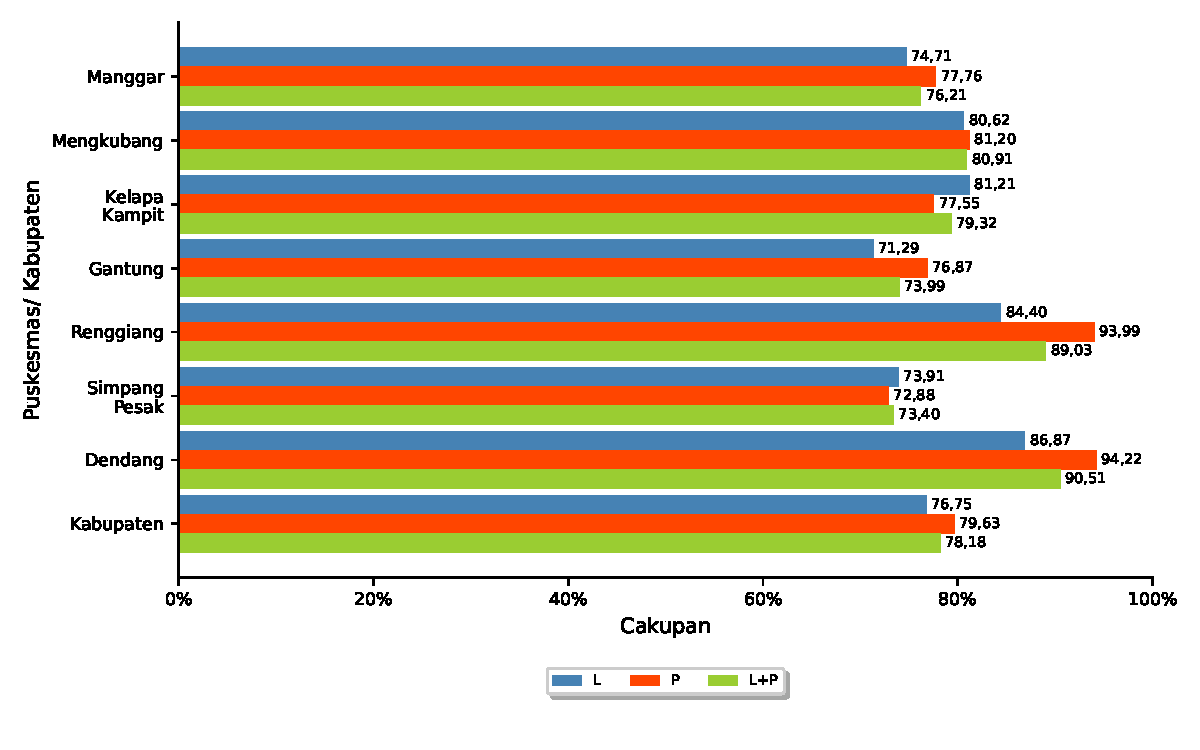
\includegraphics[width=0.85\textwidth]{bab_05/bab_05_24_balitaDitimbang}
  \caption{Cakupan Balita Ditimbang di Kab. Belitung Timur Tahun \tP per Puskesmas}
  \label{fig:Cakupan-Balita-Ditimbang}
\end{figure}


\subsection{Penemuan Kasus Balita Gizi Kurang, Balita Pendek, dan Balita Kurus}
\label{subsec:Penemuan-Kasus-Gizi-Kurang}
Balita Berat Badan Kurang adalah balita dengan status gizi yang didasarkan pada indeks berat badan menurut umur (BB/U) yang merupakan gabungan dari istilah gizi buruk dan gizi kurang dengan Z score < -2 standar deviasi, di mana Z score adalah nilai simpangan berat badan atau tinggi badan dari nilai berat badan atau tinggi badan normal menurut baku pertumbuhan WHO.
Balita Pendek adalah balita dengan status gizi yang didasarkan pada indeks panjang badan menurut umur (PB/U) atau tinggi badan menurut umur (TB/U) dengan Z score < -2 standar deviasi.
Balita Gizi Kurang adalah balita dengan status gizi yang didasarkan pada indeks berat badan menurut panjang badan (BB/PB) atau berat badan menurut tinggi badan (BB/TB) dengan Z score -2 hingga -3 standar deviasi.
Balita Gizi Buruk adalah balita dengan status gizi yang didasarkan pada indeks berat badan menurut panjang badan (BB/PB) atau berat badan menurut tinggi badan (BB/TB) dengan Z score < -3 standar deviasi.

\begin{figure}[H]
  \centering
  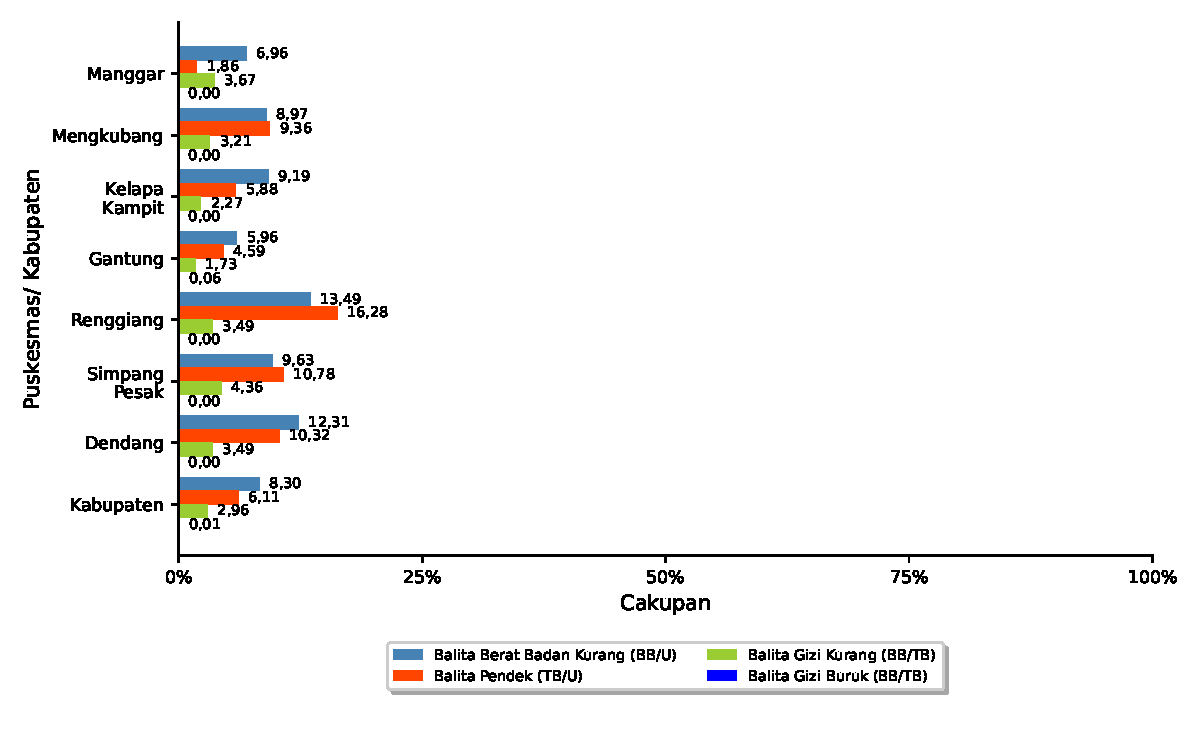
\includegraphics[width=0.85\textwidth]{bab_05/bab_05_25_statusGiziBalita}
  \caption{Sebaran Status Gizi Balita Berdasarkan Indeks BB/U, TB/U, dan BB/TB di Kab. Belitung Timur Tahun \tP per
Puskesmas}
  \label{fig:Status-Gizi-Balita}
\end{figure}

Pada tahun \tP, tercatat bahwa kasus Balita Berat Badan Kurang (BB/U) berjumlah 583 kasus atau 8,30\% dari jumlah balita ditimbang.
Kasus Balita Pendek (TB/U) atau \textit{stunting} berjumlah 429 kasus atau 6,11\% dari jumlah balita ditimbang.
Kasus Balita Gizi Kurang (BB/TB) berjumlah 208 kasus atau 2,96 \% dari jumlah balita ditimbang.
Kasus Balita Gizi Buruk (BB/TB) berjumlah 1 kasus atau 0,01 \% dari jumlah balita ditimbang (\autoref{fig:Status-Gizi-Balita}).

\subsection{Kesehatan Anak Usia Sekolah}
\subsubsection{Penjaringan Kesehatan Siswa SD, SMP, SMA}
Penjaringan kesehatan siswa SD/ MI adalah pemeriksaan kesehatan umum terhadap murid kelas 1 SD, MI atau setingkat yang dilaksanakan oleh tenaga kesehatan bersama kader kesehatan sekolah yang mencakup minimal pemeriksaan status gizi (TB,BB), pemeriksaan gigi, tajam penglihatan dan tajam pendengaran di satu wilayah kerja pada kurun waktu tertentu.

Cakupan penjaringan kesehatan siswa SD/ MI di Kabupaten Belitung Timur pada tahun \tP adalah sebesar 100,00\%.

Penjaringan kesehatan siswa SMP dan setingkat adalah pemeriksaan kesehatan umum terhadap murid kelas 7 SMP, MTs atau setingkat yang dilaksanakan oleh tenaga kesehatan bersama kader kesehatan sekolah yang mencakup minimal pemeriksaan status gizi (TB,BB), pemeriksaan gigi, tajam penglihatan dan tajam pendengaran di satu wilayah kerja pada kurun waktu tertentu.

Cakupan penjaringan kesehatan siswa SMP/ MTs di Kabupaten Belitung Timur pada tahun \tP adalah sebesar 100,00\%.

Penjaringan kesehatan siswa SMA/ MA adalah pemeriksaan kesehatan umum terhadap murid kelas 10 SMA, MA atau setingkat yang dilaksanakan oleh tenaga kesehatan bersama kader kesehatan sekolah yang mencakup minimal pemeriksaan status gizi (TB,BB), pemeriksaan gigi, tajam penglihatan dan tajam pendengaran di satu wilayah kerja pada kurun waktu tertentu.

Cakupan penjaringan kesehatan siswa SMA/ MA di Kabupaten Belitung Timur pada tahun \tP adalah sebesar 100,00\%.

\begin{figure}[H]
    \centering
    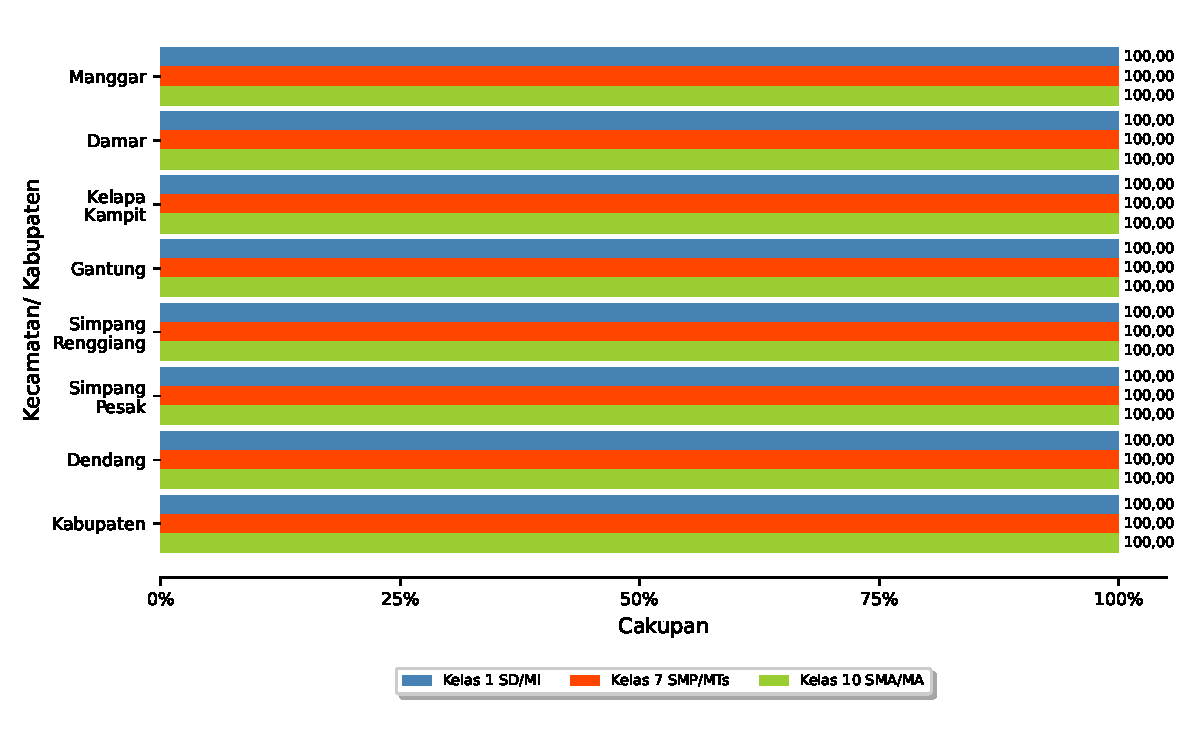
\includegraphics[width=0.85\textwidth]{bab_05/bab_05_26_kesehatanSiswa}
    \caption{Cakupan Penjaringan Kesehatan Siswa SD/ MI, SMP/ MTs, SMA/ MA di Kab. Belitung Timur Tahun \tP per Kecamatan}
    \label{fig:Cakupan-Penjaringan-Siswa}
\end{figure}

Pelayanan kesehatan usia pendidikan dasar sesuai standar meliputi :
\begin{enumerate}
    \item Skrining kesehatan.
    \item Tindaklanjut hasil skrining kesehatan.
\end{enumerate}
yang dilakukan pada anak kelas 1 sampai dengan kelas 9 di sekolah minimal satu kali dalam satu tahun ajaran dan usia 7 sampai 15 tahun diluar sekolah.

Cakupan pelayanan kesehatan usia pendidikan dasar di Kabupaten Belitung Timur pada tahun \tP adalah sebesar 100,00\% (\autoref{fig:Cakupan-Pelayanan-Kesehatan-Usia-Dikdas}).

\begin{figure}[H]
    \centering
    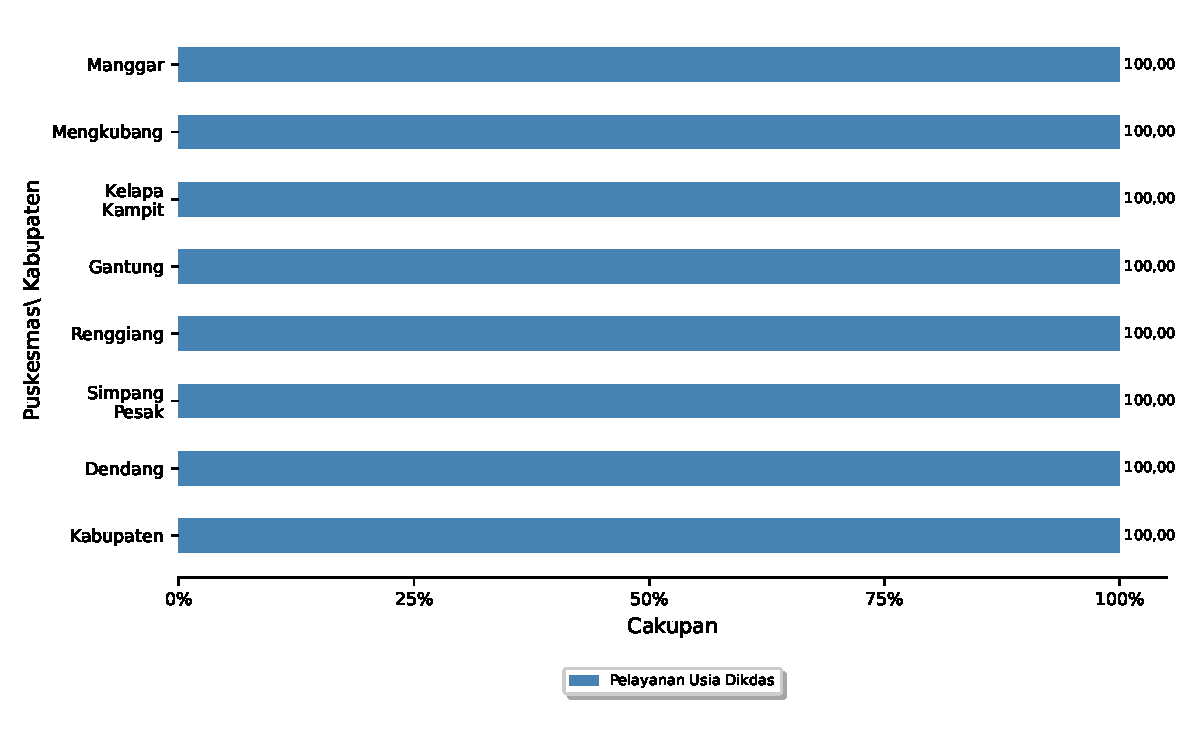
\includegraphics[width=0.85\textwidth]{bab_05/bab_05_26_kesehatanSiswa_spm}
    \caption{Cakupan Pelayanan Kesehatan Usia Pendidikan Dasar di Kab. Belitung Timur Tahun \tP per Kecamatan}
    \label{fig:Cakupan-Pelayanan-Kesehatan-Usia-Dikdas}
\end{figure}

\subsubsection{Imunisasi Anak Usia Sekolah Dasar}
Imunisasi anak usia sekolah dasar mencakup imunisasi MR dan DT pada anak usia kelas 1 SD/ sederajat, Td pada anak usia kelas 2 SD/ sederajat, Td pada anak usia kelas 5 SD/ sederajat serta HPv pada anak perempan usia kelas 5 SD/ sederajat.

Cakupan imunisasi anak usia sekolah dasar di Kabupaten Belitung Timur pada tahun \tP adalah sebesar 93,23\% (\autoref{fig:Cakupan-Imunisasi-Dasar-SD}).

\begin{figure}[!htb]
	\centering
	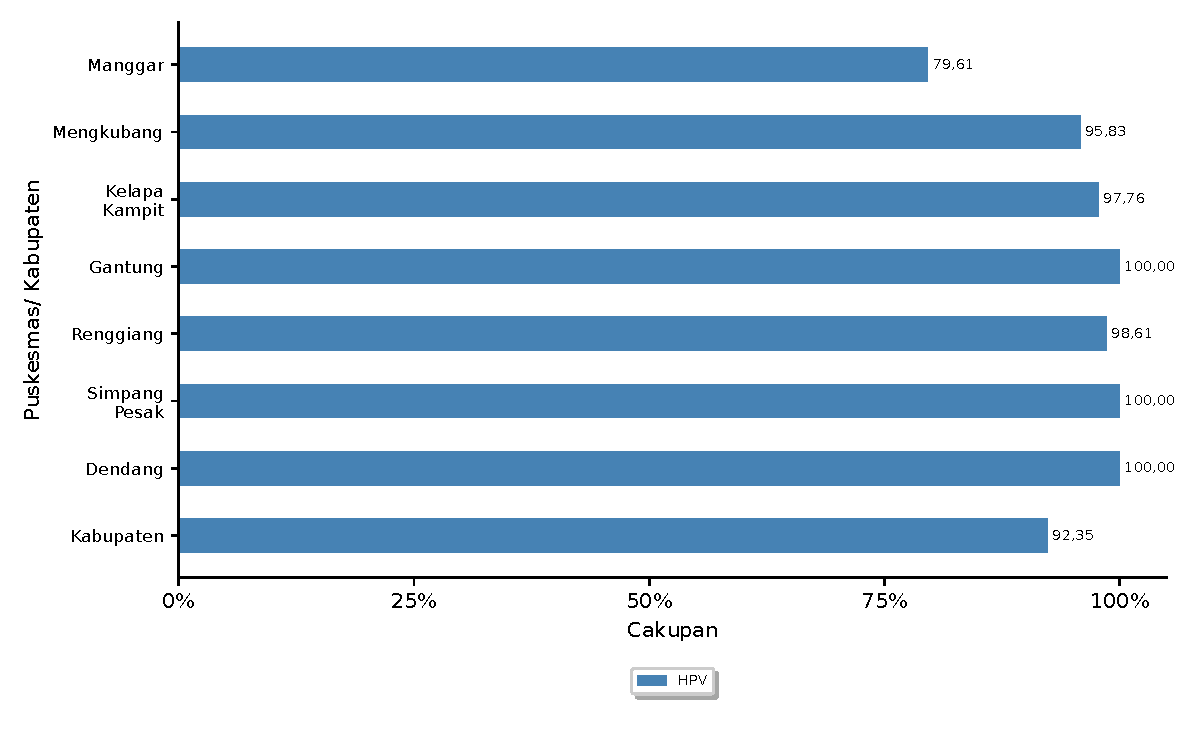
\includegraphics[width=0.85\textwidth]{bab_05/bab_05_26c_imunSD_HPV}
	\caption{Cakupan Imunisasi HPV Usia Sekolah Dasar/ Sederajat di Kab. Belitung Timur Tahun \tP per Kecamatan}
	\label{fig:Cakupan-Imunisasi-HPV-SD}
\end{figure}

\begin{figure}[!htb]
	\centering
	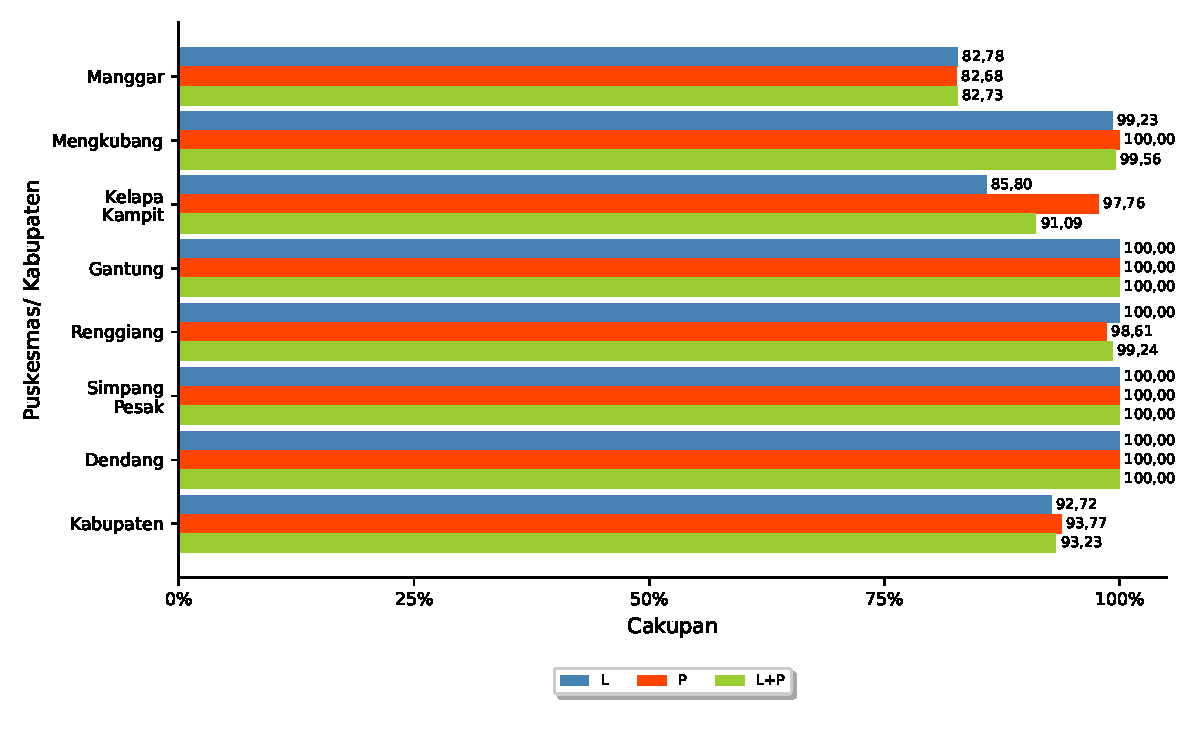
\includegraphics[width=0.85\textwidth]{bab_05/bab_05_26c_imunSD_IDL}
	\caption{Cakupan Imunisasi Usia Sekolah Dasar Lengkap di Kab. Belitung Timur Tahun \tP per Kecamatan}
	\label{fig:Cakupan-Imunisasi-Dasar-SD}
\end{figure}

\section{KESEHATAN GIGI DAN MULUT}
\subsection{Pelayanan Kesehatan Gigi dan Mulut}
Setiap penyelenggaraan upaya kesehatan gigi dan mulut yang dilakukan untuk meningkatkan kesehatan gigi dan mulut, mencegah dan menyembuhkan penyakit serta memulihkan kesehatan gigi dan mulut perorangan, keluarga, kelompok atau masyarakat secara paripurna, terpadu dan berkualitas.
Pelayanan kesehatan gigi dan mulut yang diberikan dapat berupa pemeriksaan, pengobatan, pencabutan gigi tetap/gigi sulung, penambalan tetap/sementara, perawatan pulpa, pembersihan karang gigi dan pembuatan gigi tiruan lepasan.

Rasio tumpatan/pencabutan adalah rasio jumlah penambalan gigi tetap terhadap jumlah pencabutan gigi tetap dalam setahun.
Cakupan kasus gigi dan mulut dirujuk adalah persentase kasus gigi dan mulut yang dikirim dari Puskesmas ke fasilitas kesehatan rujukan tingkat lanjut dalam satu tahun terhadap jumlah kunjungan baru dan lama rawat jalan gigi dan mulut di puskesmas meliputi pemeriksaan, pengobatan dan perawatan gigi dan mulut dalam satu tahun.

Rasio tumpatan/pencabutan di Kabupaten Belitung Timur pada tahun \tP adalah sebesar 1,64 (\autoref{fig:Cakupan-Pelayanan-Kesehatan-Gigi-Mulut-Tumpatan}).

\begin{figure}[H]
	\centering
	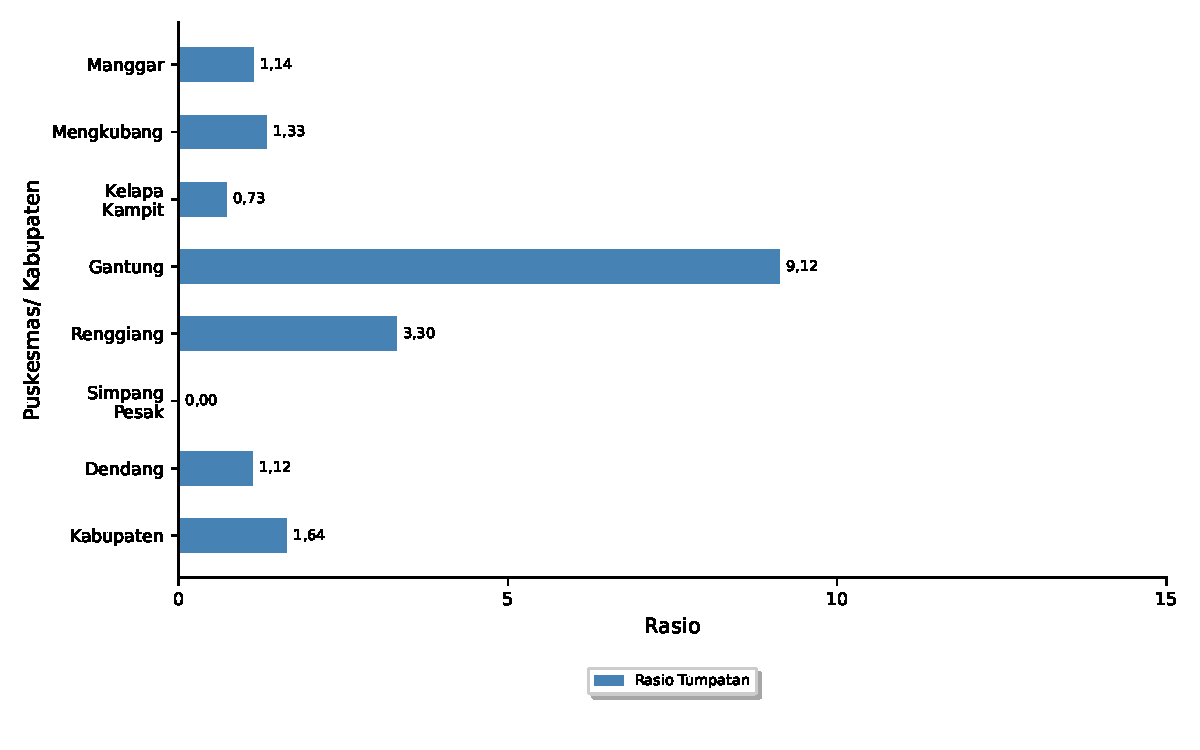
\includegraphics[width=0.85\textwidth]{bab_05/bab_05_27a_gimulTumpatan}
	\caption{Rasio Tumpatan/Pencabutan di Kab. Belitung Timur Tahun \tP per Puskesmas}
	\label{fig:Cakupan-Pelayanan-Kesehatan-Gigi-Mulut-Tumpatan}
\end{figure}

Cakupan kasus gigi dan mulut dirujuk di Kabupaten Belitung Timur pada tahun \tP adalah sebesar 7,05\% (\autoref{fig:Cakupan-Pelayanan-Kesehatan-Gigi-Mulut-Dirujuk}).

\begin{figure}[H]
	\centering
    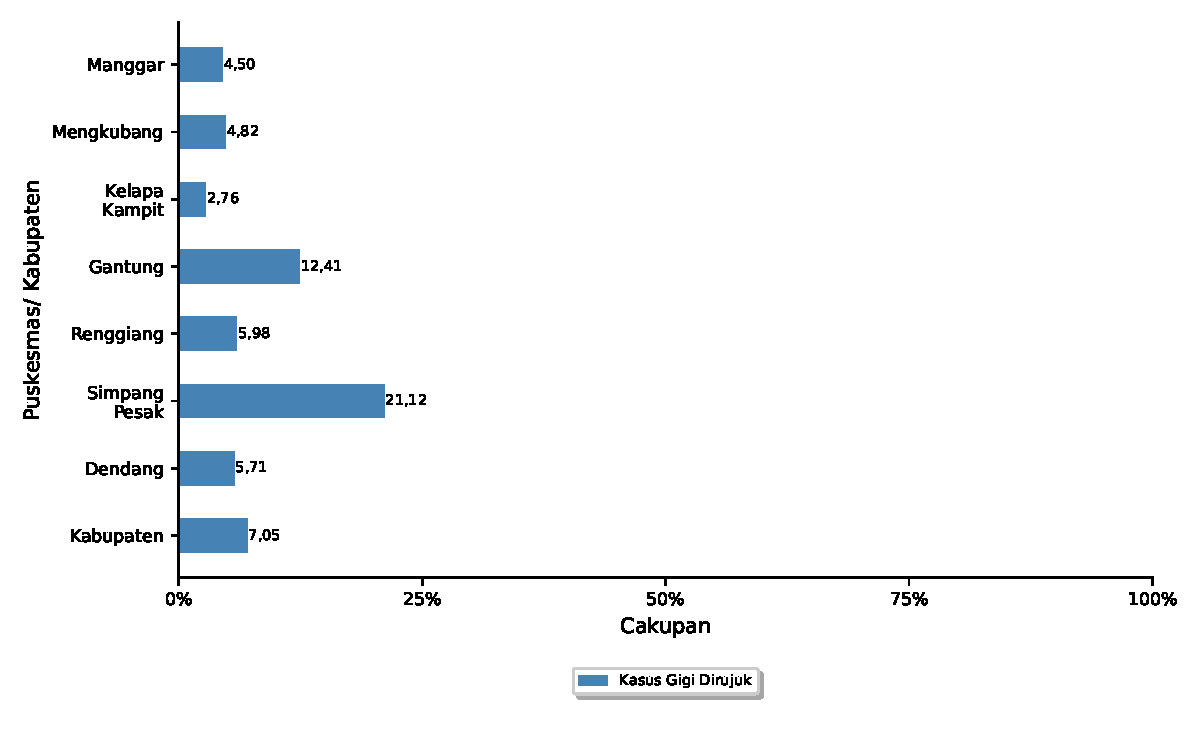
\includegraphics[width=0.85\textwidth]{bab_05/bab_05_27b_gimulDirujuk}
	\caption{Cakupan Kasus Gigi dan Mulut Dirujuk di Kab. Belitung Timur Tahun \tP per Puskesmas}
	\label{fig:Cakupan-Pelayanan-Kesehatan-Gigi-Mulut-Dirujuk}
\end{figure}

\subsection{Upaya Kesehatan Gigi Sekolah}
Penyelenggaraan upaya kesehatan gigi dan mulut anak sekolah tingkat dasar (SD/MI) atau UKGS dilakukan dengan mengutamakan pendekatan promotif dan preventif tanpa mengabaikan pendekatan kuratif dan rehabilitatif.
Perawatan kesehatan gigi dan mulut diberikan kepada murid SD/MI dalam bentuk preventif (\textit{topical fluoride}, \textit{surface protection}/\textit{fissure sealent} atau \textit{atraumatic restoration treatment}) dan kuratif sederhana seperti pengobatan, penambalan gigi, dan pencabutan gigi sulung maupun tetap yang dilakukan baik di sekolah maupun Puskesmas.

Cakupan SD/ MI di Kabupaten Belitung Timur mendapat pelayanan gigi pada tahun \tP adalah sebesar 92,45\% (\autoref{fig:Cakupan-SD-Mendapat-Pelayanan-Gigi}).

\begin{figure}[H]
	\centering
	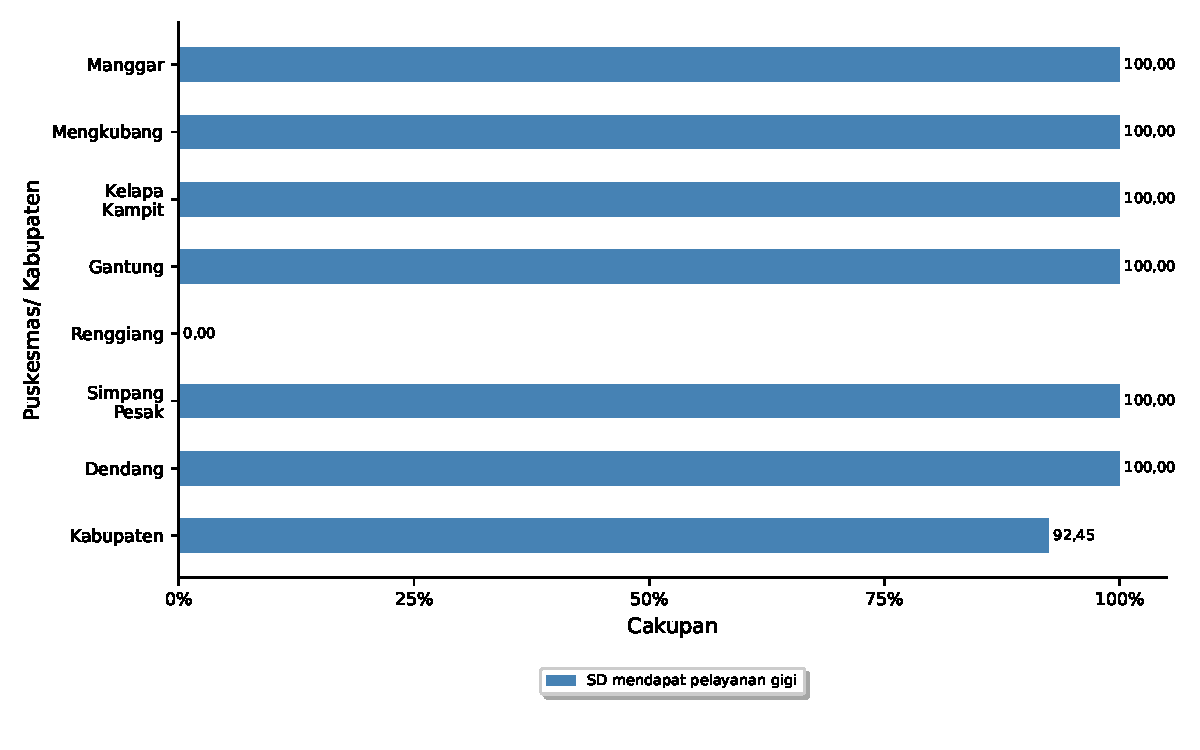
\includegraphics[width=0.85\textwidth]{bab_05/bab_05_27c_SDpelayananGigi}
	\caption{Cakupan Pemeriksaan Gigi dan Mulut Murid SD/MI di Kab. Belitung Timur Tahun \tP per Puskesmas}
	\label{fig:Cakupan-SD-Mendapat-Pelayanan-Gigi}
\end{figure}

Cakupan murid SD/MI mendapat perawatan setelah pemeriksaan di Kabupaten Belitung Timur pada tahun \tP adalah sebesar 45,91\% (\autoref{fig:Cakupan-Pelayanan-Kesehatan-Gigi-Mulut-SD-Dirawat}).

\begin{figure}[H]
	\centering
	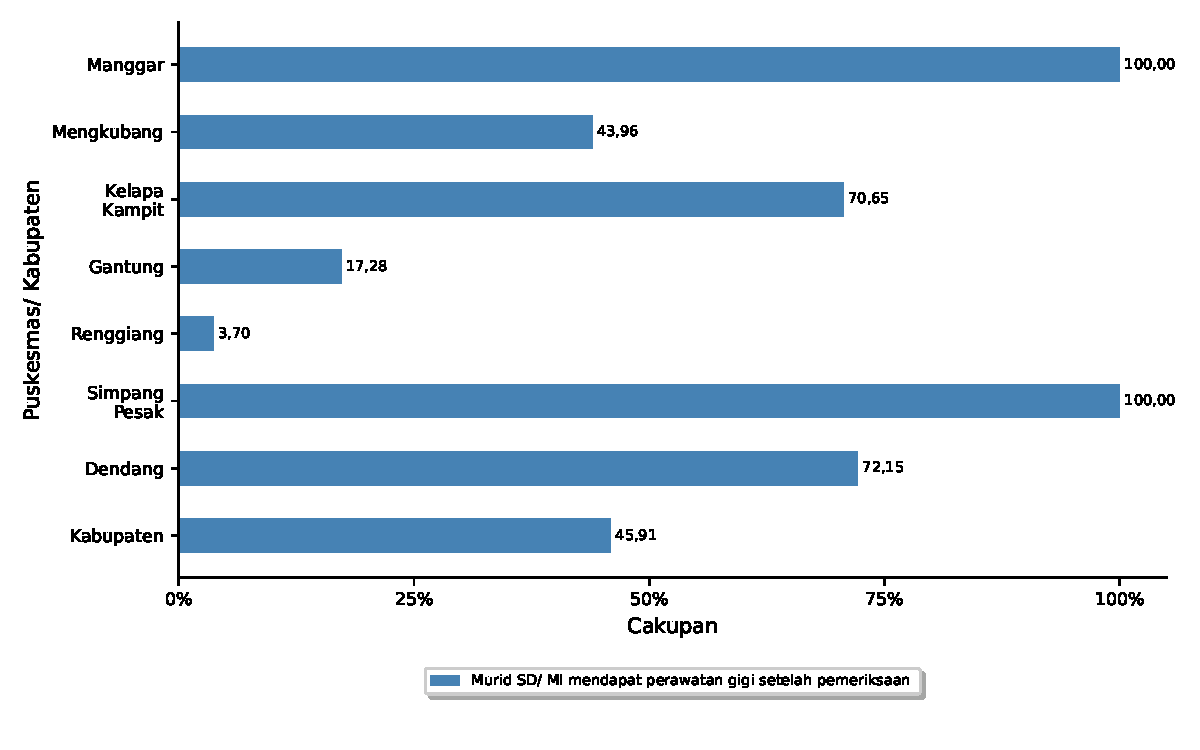
\includegraphics[width=0.85\textwidth]{bab_05/bab_05_27d_gimulSDdirawat}
	\caption{Cakupan Perawatan Gigi dan Mulut Murid SD/MI di Kab. Belitung Timur Tahun \tP per Puskesmas}
	\label{fig:Cakupan-Pelayanan-Kesehatan-Gigi-Mulut-SD-Dirawat}
\end{figure}

\section[USIPRO DAN USILA]{KESEHATAN USIA PRODUKTIF DAN USIA LANJUT}
\subsection{Pelayanan Kesehatan Usia Produktif}
Cakupan pelayanan kesehatan usia produktif adalah cakupan penduduk usia 15–59 tahun yang mendapat pelayanan skrining kesehatan sesuai standar di wilayah kerjanya dalam kurun waktu satu tahun. Edukasi dilaksanakan di Fasilitas Pelayanan Kesehatan dan/ atau UKBM dan/ atau kunjungan rumah. Pelayanan kesehatan sesuai standar meliputi:
\begin{enumerate}
  \item Edukasi kesehatan termasuk keluarga berencana;
  \item Skrining faktor risiko penyakit menular dan penyakit tidak menular:
  \begin{enumerate}
    \item Pengukuran tinggi badan, berat badan, dan lingkar perut;
    \item Pengukuran tekanan darah;
    \item Pemeriksaan gula darah; dan
    \item Anamnesa perilaku berisiko.
  \end{enumerate}
\end{enumerate}

Cakupan pelayanan kesehatan usia produktif di Kabupaten Belitung Timur pada tahun \tP adalah 96,56\%.
%, meningkat dari cakupan tahun 2021 sebesar 65,23\%.
Dari 87.564 orang penduduk yang diskrining, sebanyak 33.163 orang (39,22\%) ditemukan beresiko PTM.

\begin{figure}[H]
    \centering
    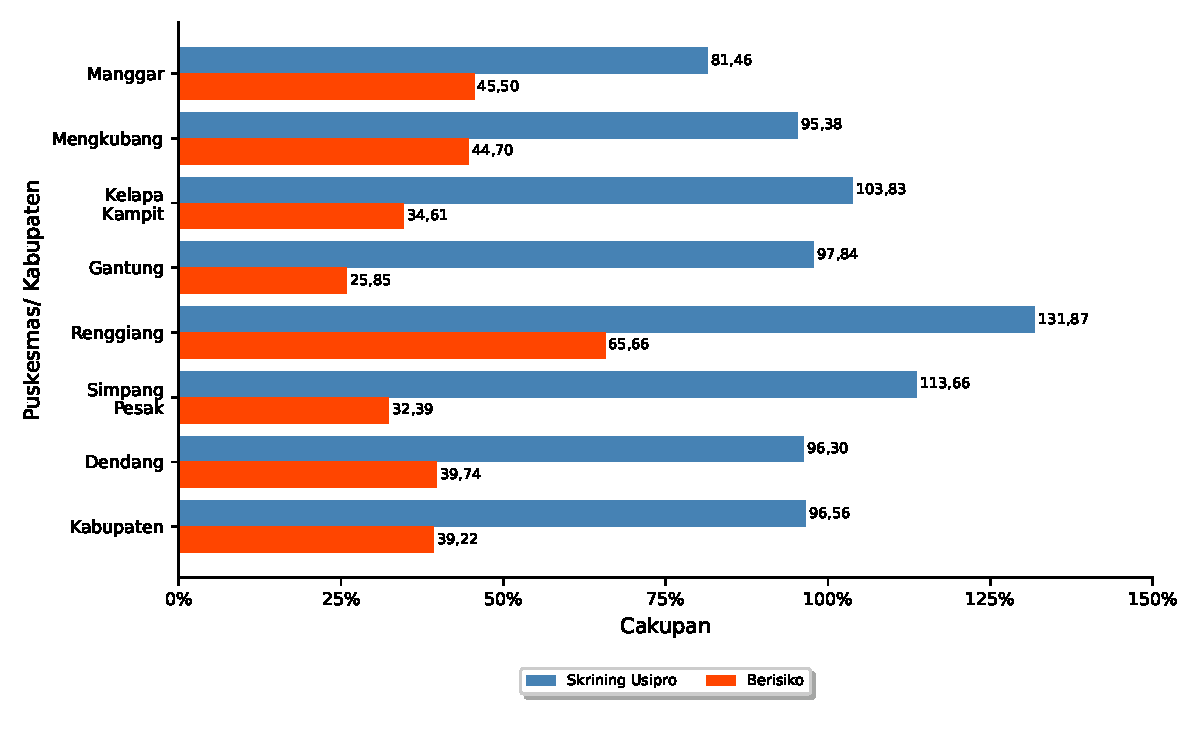
\includegraphics[width=0.85\textwidth]{bab_05/bab_05_28_skriningProduktif}
    \caption{Cakupan Pelayanan Kesehatan Usia Produktif dan Penemuan Risiko PTM di Kab. Belitung Timur Tahun \tP per Puskesmas}
    \label{fig:Cakupan-Yankes-Usprod}
\end{figure}

\subsection{Pelayanan Kesehatan Calon Pengantin}
Calon pengantin (catin) merupakan kelompok sasasan yang perlu mendapatkan intervensi dalam pelayanan kesehatan reproduksi.
Pemberian KIE kesehatan reproduksi kepada calon pengantin merupakan salah satu upaya strategis untuk meningkatkan derajat kesehatan ibu dan bayi baru lahir melalui peningkatan pengetahuan calon pengantin agar kelak dapat merencanakan kehamilan yang sehat dan melahirkan generasi penerus yang berkualitas.

Cakupan pelayanan kesehatan calon pengantin di Kabupaten Belitung Timur pada tahun \tP adalah 100,00\% (\autoref{fig:Cakupan-Yankes-Catin}).

\begin{figure}[H]
	\centering
	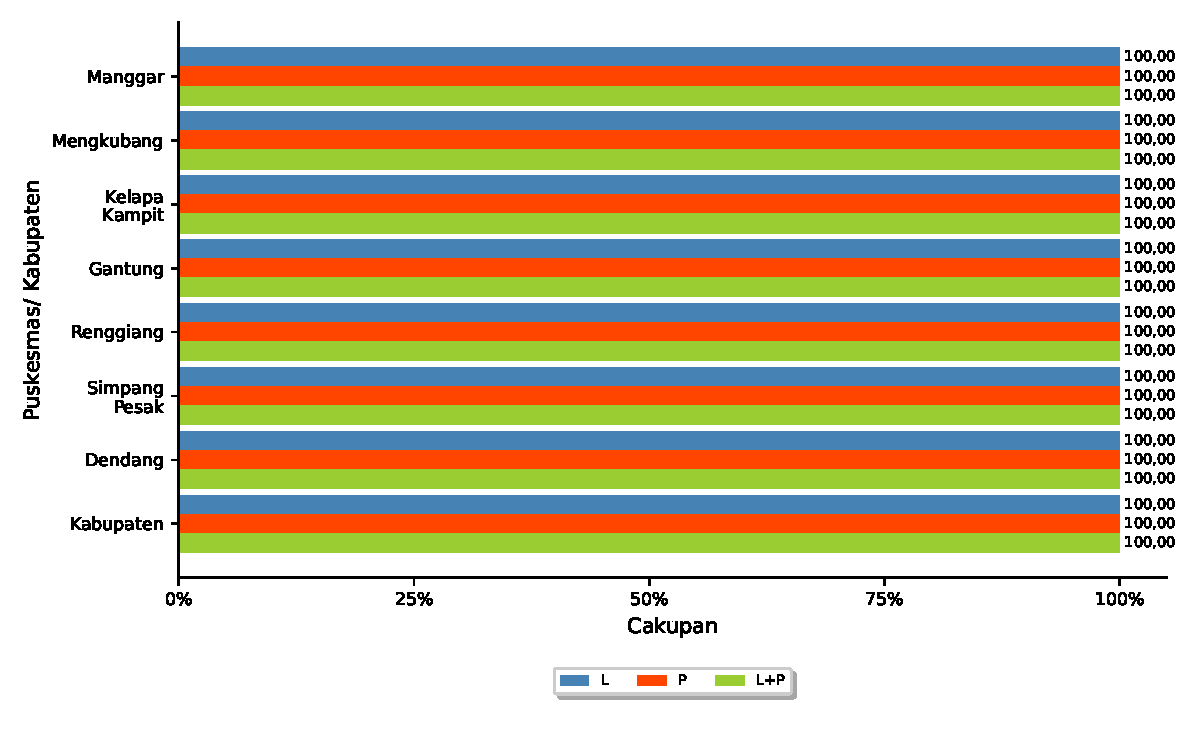
\includegraphics[width=0.85\textwidth]{bab_05/bab_05_29a_pelayananCatin}
	\caption{Cakupan Pelayanan Kesehatan Calon Pengantin di Kab. Belitung Timur Tahun \tP per Puskesmas}
	\label{fig:Cakupan-Yankes-Catin}
\end{figure}

Dari 824 catin perempuan yang diperiksa, ditemukan 245 orang (29,73\%) yang mengidap anemia dan 132 orang (16,02\%) yang mengalami gizi kurang.

\begin{figure}[H]
	\centering
	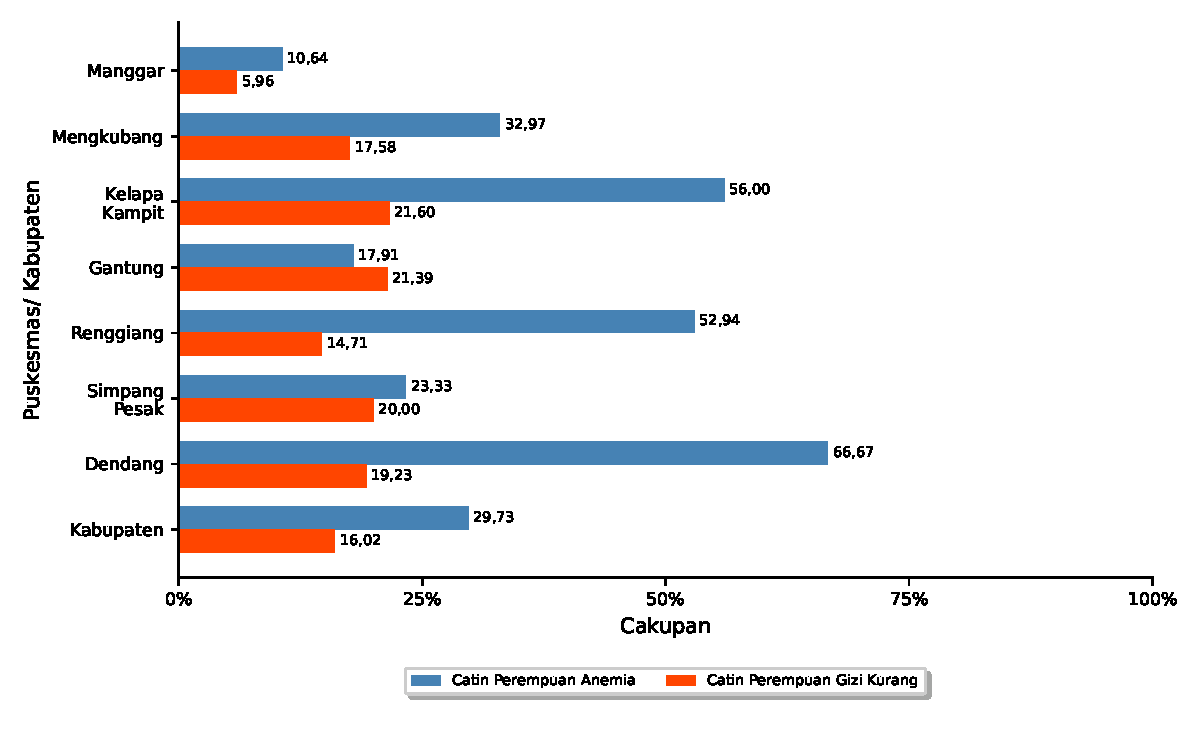
\includegraphics[width=0.85\textwidth]{bab_05/bab_05_29b_catinResiko}
	\caption{Penemuan Catin Perempuan Anemia dan Gizi Kurang di Kab. Belitung Timur Tahun \tP per Puskesmas}
	\label{fig:Cakupan-Yankes-Catin-Anemia}
\end{figure}

\subsection{Pelayanan Kesehatan Usia Lanjut}
Cakupan pelayanan kesehatan usia lanjut adalah pelayanan kesehatan untuk warga negara usia 60 tahun ke atas dalam bentuk edukasi dan skrining usia
lanjut sesuai standar pada satu wilayah kerja dalam kurun waktu satu tahun. Edukasi dilaksanakan di Fasilitas Pelayanan Kesehatan dan/atau UKBM dan/atau kunjungan rumah. Komponen skrining kesehatan yang dilakukan pada usia lanjut terdiri dari:
\begin{enumerate}
  \item Pengukuran tinggi badan, berat badan, dan lingkar perut;
  \item Pengukuran tekanan darah;
  \item Pemeriksaan gula darah;
  \item Pemeriksaan gangguan mental;
  \item Pemeriksaan gangguan kognitif;
  \item Pemeriksaan tingkat kemandirian usia lanjut; dan
  \item Anamnesa perilaku berisiko.
\end{enumerate}

Cakupan pelayanan kesehatan usia lanjut di Kabupaten Belitung Timur pada tahun \tP adalah 82,42\% (\autoref{fig:Cakupan-Yankes-Usila}).
% menurun dari cakupan tahun 2021 sebesar 69,55\%.

\begin{figure}[H]
    \centering
    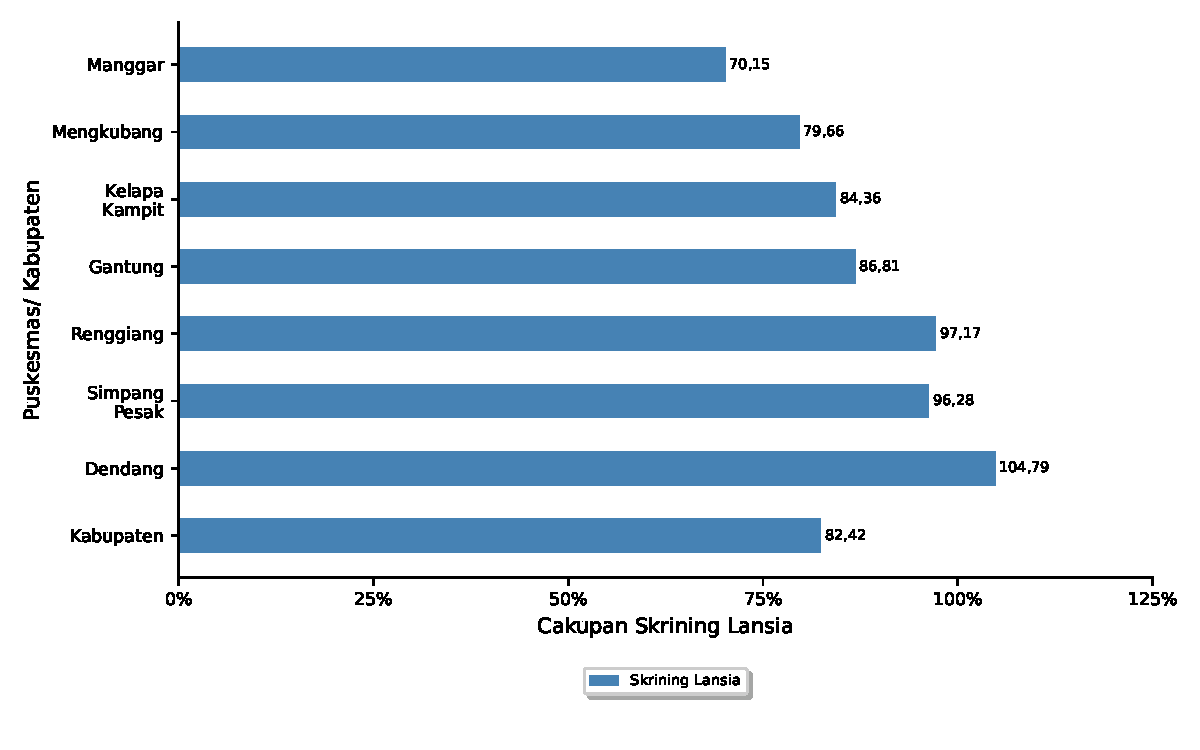
\includegraphics[width=0.85\textwidth]{bab_05/bab_05_30_skriningLansia}
    \caption{Cakupan Pelayanan Kesehatan Usia Lanjut di Kab. Belitung Timur Tahun \tP per Puskesmas}
    \label{fig:Cakupan-Yankes-Usila}
\end{figure}

%\cleardoublepage
\include{bab_06/bab_06_pengendalian_penyakit}
%\cleardoublepage
%\include{bab_07/bab_07_kesehatan_lingkungan}
\cleardoublepage
%\include{bab_08/bab_08_penutup}
%\cleardoublepage
%renewcommand for appendixtoc should be placed before appendices section
\renewcommand\appendixtocname{Lampiran}
{\sffamily
\begin{appendices}
\begin{landscape}
%	\chapter{Standar Pelayanan Minimal}
\begin{center}
\renewcommand*{\arraystretch}{1.3}
%\newcolumntype{R}[1]{>{\raggedleft\arraybackslash}p{#1}}
\begin{longtable}{rY{20em}Z{6em}Z{6em}Z{6em}Z{8em}Z{7em}}
% prevent longtable show up twice in TOC. set caption for firsthead, then set empty starred
% caption for next heads. in longtable \toprule should be prepended by \\
\caption{Capaian Standar Pelayanan Minimal (SPM) Bidang Kesehatan Kab. Belitung Timur Tahun \tP}
\\ \toprule
\multirow{2}[0]{*}{No} & \multirow{2}[0]{*}{JENIS PELAYANAN{*}} & \multicolumn{3}{c}{MUTU LAYANAN} & \multirow{2}[0]{7em}{\raggedleft MUTU BARANG/ JASA/ SDM (\%)} & \multirow{2}[0]{6em}{\raggedleft MUTU SPM (\%){***}}\\
\cmidrule(l{2pt}r{2pt}){3-5}
   &                    & PEMBILANG & PENYEBUT{**} & MUTU (\%) &                             &                   \\
\midrule
\endfirsthead
\caption*{}
\\ \toprule
\multirow{2}[0]{*}{No} & \multirow{2}[0]{*}{JENIS PELAYANAN{*}} & \multicolumn{3}{c}{MUTU LAYANAN} & \multirow{2}[0]{7em}{\raggedleft MUTU BARANG/ JASA/ SDM (\%)} & \multirow{2}[0]{6em}{\raggedleft MUTU SPM (\%){***}}\\
\cmidrule(l{2pt}r{2pt}){3-5}
&                    & PEMBILANG & PENYEBUT{**} & MUTU (\%) &                             &                   \\
\midrule
\endhead

 1 & Pelayanan kesehatan ibu hamil                          &  1.546 &  1.843 &  83,48 & 100,00 &  87,11 \\
 2 & Pelayanan kesehatan ibu bersalin                       &  1.666 &  1.843 &  90,40 & 100,00 &  92,32 \\
 3 & Pelayanan kesehatan bayi baru lahir                    &  1.646 &  1.843 &  89,31 & 100,00 &  91,45 \\
 4 & Pelayanan kesehatan balita                             &  7.632 &  8.823 &  86,50 & 100,00 &  89,20 \\
 5 & Pelayanan kesehatan pada usia pendidikan dasar         & 18.982 & 19.640 &  96,65 & 100,00 &  97,32 \\
 6 & Pelayanan kesehatan pada usia produktif                & 84.550 & 87.514 &  96,61 & 100,00 &  97,29 \\
 7 & Pelayanan kesehatan pada usia lanjut                   & 11.881 & 14.379 &  82,63 & 100,00 &  86,10 \\
 8 & Pelayanan kesehatan penderita hipertensi               & 20.853 & 24.256 &  85,97 & 100,00 &  88,78 \\
 9 & Pelayanan kesehatan penderita diabetes melitus         &  2.338 &  2.445 &  95,62 & 100,00 &  96,50 \\
10 & Pelayanan kesehatan orang dengan gangguan jiwa berat   &    320 &    320 & 100,00 & 100,00 & 100,00 \\
11 & Pelayanan kesehatan orang terduga tuberkulosis         &  2.482 &  2.262 & 100,00 & 100,00 & 100,00 \\
12 & Pelayanan kesehatan orang dengan risiko terinfeksi HIV &  2.742 &  3.105 &  88,31 & 100,00 &  90,65 \\
\midrule
\multicolumn{2}{r}{Indeks SPM{****}}                        &        &        &        &        & 93,06 \\
                                                     \multicolumn{7}{r}{TUNTAS UTAMA} \\
\bottomrule
\end{longtable}
\par\end{center}


{*}) \emph{Sesuai Peraturan Menteri Kesehatan Nomor 6 Tahun 2024 tentang Standar Teknis Pemenuhan Mutu Pelayanan Dasar Pada Standar Pelayanan
Minimal Bidang Kesehatan}

{**}) \emph{Berdasarkan estimasi dan tidak selalu menggambarkan jumlah yang sebenarnya di populasi}

{***}) \emph{Dihitung dari komponen mutu layanan dan komponen mutu barang/jasa/SDM}

{****}) \emph{Sesuai Peraturan Menteri Dalam Negeri Nomor 59 Tahun 2021 Tentang Penerapan Standar Pelayanan Minimal}
 %done
\end{landscape}
%\cleardoublepage
%\include{bab_09_apendiks/bab_09_apendiks_2_sdgs}
%\cleardoublepage
%\include{bab_09_apendiks/bab_09_apendiks_3_iku}
%\cleardoublepage
\chapter{Tabel Profil}
%    \phantomsection
\addcontentsline{lot}{chapter}{\protect\numberline{}Resume Profil}

% Table generated by Excel2LaTeX from sheet 'Resume (unformatted)'
\begin{small}
\begin{longtable}{rY{12em}rrrrY{5em}Y{5em}}
    \multicolumn{8}{c}{RESUME PROFIL KESEHATAN}\\
    \multicolumn{8}{c}{KABUPATEN BELITUNG TIMUR}\\
    \multicolumn{8}{c}{TAHUN \tP}\\
	\\ \toprule

	\multirow{2}{*}{\textbf{No}} & \multirow{2}{*}{\textbf{INDIKATOR}}                & \multicolumn{5}{c}{\textbf{ANGKA/ NILAI}} & \multirow{2}{5em}{\raggedright\textbf{No. Lampiran}} \\
    \cmidrule{3-7}
	&                                                                                 & \textbf{L} & \textbf{P} & \textbf{L + P} & \textbf{Jumlah} & \textbf{Satuan} & \\ \midrule
	\endfirsthead
	\\ \toprule
	\multirow{2}{*}{\textbf{No}} & \multirow{2}{*}{\textbf{INDIKATOR}}                & \multicolumn{5}{c}{\textbf{ANGKA/ NILAI}} & \multirow{2}{5em}{\raggedright\textbf{No. Lampiran}} \\
    \cmidrule{3-7}
    &                                                                                 & \textbf{L} & \textbf{P} & \textbf{L + P} & \textbf{Jumlah} & \textbf{Satuan} & \\ \midrule
    \endhead
    % make bottom border on when table continue to next page
    \midrule
    \endfoot
    \endlastfoot
	           \textbf{I} & \textbf{GAMBARAN UMUM}                                                                                  &        &        &         &                    &                                &          \\
	                    1 & Luas Wilayah                                                                                            &        &        &         &              2.507 & Km\textsuperscript{2}          & Tabel 1  \\
	  \rowcolor{black!5}2 & Jumlah Desa/ Kelurahan                                                                                  &        &        &         &                 39 & Desa/Kelurahan                 & Tabel 1  \\
	                    3 & Jumlah Penduduk                                                                                         & 69.252 & 65.573 & 134.825 &                    & Jiwa                           & Tabel 2  \\
	  \rowcolor{black!5}4 & Rata-rata jiwa/ rumah tangga                                                                            &        &        &         &               3,23 & Jiwa                           & Tabel 1  \\
	                    5 & Kepadatan Penduduk /Km\textsuperscript{2}                                                               &        &        &         &              53,78 & Jiwa/Km\textsuperscript{2}     & Tabel 1  \\
	  \rowcolor{black!5}6 & Rasio Beban Tanggungan                                                                                  &        &        &         &              45,70 & per 100 penduduk produktif     & Tabel 2  \\
	                    7 & Rasio Jenis Kelamin                                                                                     &        &        &         &             105,61 &                                & Tabel 2  \\
	  \rowcolor{black!5}8 & Persentase Penduduk 15 tahun ke atas melek huruf                                                        &   0,00 &   0,00 &   99,14 &                    & \%                             & Tabel 3  \\
	                      &                                                                                                         &        &        &         &                    &                                &          \\
	          \textbf{II} & \textbf{SARANA KESEHATAN}                                                                               &        &        &         &                    &                                &          \\
	        \textbf{II.1} & \textbf{Sarana Kesehatan}                                                                               &        &        &         &                    &                                &          \\
	                    9 & Jumlah Rumah Sakit Umum                                                                                 &        &        &         &                  1 & RS                             & Tabel 4  \\
	 \rowcolor{black!5}10 & Jumlah Rumah Sakit Khusus                                                                               &        &        &         &                  0 & RS                             & Tabel 4  \\
	                   11 & Jumlah Puskesmas Rawat Inap                                                                             &        &        &         &                  4 & Puskesmas                      & Tabel 4  \\
	 \rowcolor{black!5}12 & Jumlah Puskesmas non-Rawat Inap                                                                         &        &        &         &                  3 & Puskesmas                      & Tabel 4  \\
	                   13 & Jumlah Puskesmas Keliling                                                                               &        &        &         &                  0 & Puskesmas keliling             & Tabel 4  \\
	 \rowcolor{black!5}14 & Jumlah Puskesmas pembantu                                                                               &        &        &         &                 39 & Pustu                          & Tabel 4  \\
	                   15 & Jumlah Apotek                                                                                           &        &        &         &                 29 & Apotek                         & Tabel 4  \\
	 \rowcolor{black!5}16 & Jumlah Klinik Pratama                                                                                   &        &        &         &                  6 & Klinik Pratama                 & Tabel 4  \\
	                   17 & Jumlah Klinik Utama                                                                                     &        &        &         &                  1 & Klinik Utama                   & Tabel 4  \\
	                      &                                                                                                         &        &        &         &                    &                                &          \\
	        \textbf{II.2} & \multicolumn{3}{Y{21em}}{\textbf{Akses dan Mutu Pelayanan Kesehatan}}                                                     &         &                    &                                &          \\
	                   18 & Cakupan Kunjungan Rawat Jalan                                                                           & 148,42 & 235,90 &  190,97 &                    & \%                             & Tabel 5  \\
	 \rowcolor{black!5}19 & Cakupan Kunjungan Rawat Inap                                                                            &   7,86 &  11,99 &    9,87 &                    & \%                             & Tabel 5  \\
	                   20 & Angka kematian kasar/ \textit{Gross Death Rate} (GDR) di RS                                             &  61,26 &  39,20 &   48,39 &                    & per 1.000 pasien keluar        & Tabel 6  \\
	 \rowcolor{black!5}21 & Angka kematian murni/ \textit{Nett Death Rate} (NDR) di RS                                              &  28,02 &  17,87 &   22,09 &                    & per 1.000 pasien keluar        & Tabel 6  \\
	                   22 & Persentase \textit{Bed Occupation Rate} (BOR) di RS                                                     &        &        &         &              54,41 & \%                             & Tabel 7  \\
	 \rowcolor{black!5}23 & \textit{Bed Turn Over (BTO)} di RS                                                                      &        &        &         &              58,43 & Kali                           & Tabel 7  \\
	                   24 & \textit{Turn of Interval (TOI)} di RS                                                                   &        &        &         &               2,85 & Hari                           & Tabel 7  \\
	 \rowcolor{black!5}25 & \textit{Average Length of Stay (ALOS)} di RS                                                            &        &        &         &               3,40 & Hari                           & Tabel 7  \\
	                   26 & Persentase Puskesmas dengan ketersediaan obat esensial \& vaksin IRL                                    &        &        &         &             100,00 & \%                             & Tabel 11 \\
	                      &                                                                                                         &        &        &         &                    &                                &          \\
	        \textbf{II.3} & \multicolumn{3}{Y{21em}}{\textbf{Upaya Kesehatan Bersumberdaya Masyarakat (UKBM)}}                                        &         &                    &                                &          \\
	                   27 & Jumlah Posyandu Siklus Hidup                                                                            &        &        &         &                134 & Posyandu                       & Tabel 12 \\
	 \rowcolor{black!5}28 & Persentase Posyandu Siklus Hidup Aktif                                                                  &        &        &         &             100,00 & \%                             & Tabel 12 \\
	                      &                                                                                                         &        &        &         &                    &                                &          \\
	         \textbf{III} & \multicolumn{3}{Y{21em}}{\textbf{SUMBER DAYA MANUSIA KESEHATAN}}                                                          &         &                    &                                &          \\
	                   29 & Rasio Dokter Spesialis per 1.000 Penduduk                                                               &        &        &         &              34,12 & per 1.000 penduduk             & Tabel 13 \\
	 \rowcolor{black!5}30 & Rasio Dokter Sub Spesialis per 1.000 Penduduk                                                           &        &        &         &               7,42 & per 1.000 penduduk             & Tabel 13 \\
	                   31 & Rasio Dokter per 1.000 Penduduk                                                                         &        &        &         &               0,74 & per 1.000 penduduk             & Tabel 13 \\
	 \rowcolor{black!5}32 & Rasio Dokter Gigi Spesialis per 1.000 Penduduk                                                          &        &        &         &               5,19 & per 1.000 penduduk             & Tabel 13 \\
	                   33 & Rasio Dokter Gigi Sub Spesialis per 1.000 Penduduk                                                      &        &        &         &               0,74 & per 1.000 penduduk             & Tabel 13 \\
	 \rowcolor{black!5}34 & Rasio Dokter Gigi per 1.000 Penduduk                                                                    &        &        &         &               0,00 & per 1.000 penduduk             & Tabel 13 \\
	                   35 & Rasio Keperawatan per 1.000 Penduduk                                                                    &        &        &         &             278,88 & per 1.000 penduduk             & Tabel 14 \\
	 \rowcolor{black!5}36 & Rasio Tenaga Kebidanan per 1.000 Penduduk                                                               &        &        &         &             114,22 & per 1.000 penduduk             & Tabel 14 \\
	                   37 & Rasio Tenaga Kesehatan Masyarakat per 1.000 Penduduk                                                    &        &        &         &              21,51 & per 1.000 penduduk             & Tabel 15 \\
	 \rowcolor{black!5}38 & Rasio Tenaga Kesehatan Lingkungan per 1.000 Penduduk                                                    &        &        &         &               6,68 & per 1.000 penduduk             & Tabel 15 \\
	                   39 & Rasio Tenaga Gizi per 1.000 Penduduk                                                                    &        &        &         &              16,32 & per 1.000 penduduk             & Tabel 15 \\
	 \rowcolor{black!5}40 & Rasio Tenaga Kefarmasian per 1.000 Penduduk                                                             &        &        &         &              27,44 & per 1.000 penduduk             & Tabel 16 \\
	                   41 & Rasio Tenaga Psikologis Klinis per 1.000 Penduduk                                                       &        &        &         &               0,74 & per 1.000 penduduk             & Tabel 16 \\
	 \rowcolor{black!5}42 & Rasio Tenaga Kesehatan Tradisional per 1.000 Penduduk                                                   &        &        &         &               0,00 & per 1.000 penduduk             & Tabel 16 \\
	                   43 & Rasio Tenaga Tehnik Biomedika per 1.000 Penduduk                                                        &        &        &         &              20,77 & per 1.000 penduduk             & Tabel 17 \\
	 \rowcolor{black!5}44 & Rasio Tenaga Tehnik Keterapian Fisik per 1.000 Penduduk                                                 &        &        &         &               8,16 & per 1.000 penduduk             & Tabel 17 \\
	                   45 & Rasio Tenaga Keteknisan Medis per 1.000 Penduduk                                                        &        &        &         &              25,96 & per 1.000 penduduk             & Tabel 17 \\
	                      &                                                                                                         &        &        &         &                    &                                &          \\
	          \textbf{IV} & \multicolumn{3}{Y{21em}}{\textbf{PEMBIAYAAN KESEHATAN}}                                                                   &         &                    &                                &          \\
	                   46 & Cakupan Jaminan Kesehatan Nasional (JKN)                                                                &        &        &         &              98,45 & \%                             & Tabel 19 \\
	 \rowcolor{black!5}47 & Total anggaran kesehatan                                                                                &        \multicolumn{4}{r}{ 220.555.334.822,00} & Rp                             & Tabel 20 \\
	                   48 & Persentase APBD kesehatan terhadap APBD Kab.                                                            &        &        &         &              25,94 & \%                             & Tabel 20 \\
	 \rowcolor{black!5}49 & Anggaran kesehatan perkapita                                                                            &               \multicolumn{4}{r}{1.635.863,79} & Rp                             & Tabel 20 \\
	                      &                                                                                                         &        &        &         &                    &                                &          \\
						  &                                                                                                         &        &        &         &                    &                                &          \\
	           \textbf{V} & \textbf{KESEHATAN KELUARGA}                                                                             &        &        &         &                    &                                &          \\
	         \textbf{V.1} & \textbf{Kesehatan Ibu}                                                                                  &        &        &         &                    &                                &          \\
	                   50 & Jumlah Lahir Hidup                                                                                      &    877 &    786 &   1.663 &                    & Orang                          & Tabel 21 \\
	 \rowcolor{black!5}51 & Angka Lahir Mati (dilaporkan)                                                                           &        &        &   10,12 &                    & per 1.000 Kelahiran Hidup      & Tabel 21 \\
	                   52 & Jumlah Kematian Ibu                                                                                     &        &      4 &         &                    & Ibu                            & Tabel 23 \\
	 \rowcolor{black!5}53 & Angka Kematian Ibu (dilaporkan)                                                                         &        & 240,53 &         &                    & per 100.000 Kelahiran Hidup    & Tabel 24 \\
	                   54 & Persentase Kunjungan Ibu Hamil (K1)                                                                     &        &  97,18 &         &                    & \%                             & Tabel 26 \\
	 \rowcolor{black!5}55 & Persentase Kunjungan Ibu Hamil (K6)                                                                     &        &  90,50 &         &                    & \%                             & Tabel 26 \\
	                   56 & Persentase Persalinan di Fasyankes                                                                      &        &  90,34 &         &                    & \%                             & Tabel 26 \\
	 \rowcolor{black!5}57 & Persentase Pelayanan Ibu Nifas KF Lengkap                                                               &        &  90,50 &         &                    & \%                             & Tabel 26 \\
	                   58 & Persentase Ibu Nifas Mendapat Vitamin A                                                                 &        &  90,50 &         &                    & \%                             & Tabel 26 \\
	 \rowcolor{black!5}59 & Persentase Ibu hamil dengan imunisasi Td2+                                                              &        &  48,21 &         &                    & \%                             & Tabel 27 \\
	                   60 & Persentase Ibu Hamil Mengonsumsi Tablet Tambah Darah 180 Tablet                                         &        &  84,09 &         &                    & \%                             & Tabel 28 \\
	 \rowcolor{black!5}61 & Persentase Bumil dengan Komplikasi Kebidanan yang Ditangani                                             &        & 170,20 &         &                    & \%                             & Tabel 32 \\
	                   62 & Persentase Peserta KB Aktif Modern                                                                      &        &        &   85,61 &                    & \%                             & Tabel 29 \\
	 \rowcolor{black!5}63 & Persentase Peserta KB Pasca Persalinan                                                                  &        &        &   76,06 &                    & \%                             & Tabel 31 \\
	                      &                                                                                                         &        &        &         &                    &                                &          \\
	         \textbf{V.2} & \textbf{Kesehatan Anak}                                                                                 &        &        &         &                    &                                &          \\
	                   64 & Jumlah Kematian Neonatal                                                                                &      3 &      8 &      11 &                    & neonatal                       & Tabel 34 \\
	 \rowcolor{black!5}65 & Angka Kematian Neonatal (dilaporkan)                                                                    &        &        &    6,61 &                    & per 1.000 Kelahiran Hidup      & Tabel 34 \\
	                   66 & Jumlah Bayi Mati                                                                                        &      7 &     11 &      18 &                    & bayi                           & Tabel 34 \\
	 \rowcolor{black!5}67 & Angka Kematian Bayi (dilaporkan)                                                                        &        &        &   10,82 &                    & per 1.000 Kelahiran Hidup      & Tabel 34 \\
	                   68 & Jumlah Balita Mati                                                                                      &      2 &      1 &       3 &                    & Balita                         & Tabel 34 \\
	 \rowcolor{black!5}69 & Persentase Angka Kematian Balita (dilaporkan)                                                           &        &        &    1,80 &                    & per 1.000 Kelahiran Hidup      & Tabel 34 \\
	                   70 & Persentase Bayi Baru Lahir Ditimbang                                                                    & 100,00 & 100,00 &  100,00 &                    & \%                             & Tabel 38 \\
	 \rowcolor{black!5}71 & Persentase Berat Badan Bayi Lahir Rendah (BBLR)                                                         &   9,12 &  11,32 &   10,16 &                    & \%                             & Tabel 38 \\
	                   72 & Persentase Kunjungan Neonatus 1 (KN 1)                                                                  &  99,89 &  99,62 &   99,76 &                    & \%                             & Tabel 39 \\
	 \rowcolor{black!5}73 & Persentase Kunjungan Neonatus 3 kali (KN Lengkap)                                                       &  98,75 &  99,11 &   98,92 &                    & \%                             & Tabel 39 \\
	                   74 & Persentase Bayi yang diberi ASI Eksklusif                                                               &        &        &   75,20 &                    & \%                             & Tabel 40 \\
	 \rowcolor{black!5}75 & Cakupan Imunisasi Campak/ Rubela pada Bayi                                                              &  86,52 &  87,15 &   86,82 &                    & \%                             & Tabel 43 \\
	                   76 & Persentase Imunisasi dasar lengkap pada bayi                                                            &  86,73 &  88,66 &   87,64 &                    & \%                             & Tabel 43 \\
	 \rowcolor{black!5}77 & Cakupan Bayi Mendapat Vitamin A                                                                         &        &        &   99,08 &                    & \%                             & Tabel 46 \\
	                   78 & Cakupan Anak Balita Mendapat Vitamin A                                                                  &        &        &   99,05 &                    & \%                             & Tabel 46 \\
	 \rowcolor{black!5}79 & Persentase Balita Mendapatkan Vitamin A                                                                 &        &        &   99,08 &                    & \%                             & Tabel 46 \\
	                   80 & Persentase Balita Memiliki Buku KIA                                                                     &        &        &   89,42 &                    & \%                             & Tabel 47 \\
	 \rowcolor{black!5}81 & Persentase Balita Dipantau Pertumbuhan dan Perkembangan                                                 &        &        &   90,97 &                    & \%                             & Tabel 47 \\
	                   82 & Persentase Balita Ditimbang (D/S)                                                                       &  76,75 &  79,63 &   78,18 &                    & \%                             & Tabel 48 \\
	 \rowcolor{black!5}83 & Persentase Balita Gizi Kurang (BB/TB)                                                                   &        &        &    2,96 &                    & \%                             & Tabel 49 \\
	                   84 & Persentase Balita Gizi Buruk (BB/TB)                                                                    &        &        &    0,01 &                    & \%                             & Tabel 49 \\
	 \rowcolor{black!5}85 & Cakupan Pemeriksaan Kesehatan Gratis Siswa Kelas 1 SD/ MI                                               &        &        &  100,00 &                    & \%                             & Tabel 50 \\
	                   86 & Cakupan Pemeriksaan Kesehatan Gratis Siswa Kelas 7 SMP/ MTs                                             &        &        &  100,00 &                    & \%                             & Tabel 50 \\
	 \rowcolor{black!5}87 & Cakupan Pemeriksaan Kesehatan Gratis Siswa Kelas 10 SMA/ MA                                             &        &        &  100,00 &                    & \%                             & Tabel 50 \\
	                   88 & Cakupan Pemeriksaan Kesehatan Gratis pada usia pendidikan dasar                                         &        &        &  100,00 &                    & \%                             & Tabel 50 \\
	 \rowcolor{black!5}89 & Cakupan Imunisasi HPV                                                                                   &        &        &   93,23 &                    & \%                             & Tabel 51 \\
	                   90 & Cakupan Imunisasi Anak Sekolah Lengkap                                                                  &  92,72 &  93,77 &   93,23 &                    & \%                             & Tabel 51 \\
	 \rowcolor{black!5}91 & Cakupan Pelayanan Kesehatan Gigi dan Mulut                                                              &        &        &    7,05 &                    & \%                             & Tabel 52 \\
	                   92 & Cakupan Pelayanan Kesehatan Gigi dan Mulut Pada Anak SD atau Setara                                     &        &        &   45,91 &                    & \%                             & Tabel 53 \\
	                      &                                                                                                         &        &        &         &                    &                                &          \\
	         \textbf{V.3} & \multicolumn{3}{Y{21em}}{\textbf{Kesehatan Usia Produktif dan Usia Lanjut}}                                               &         &                    &                                &          \\
	                   93 & Persentase Pelayanan Kesehatan Usia Produktif                                                           &        &        &   96,56 &                    & \%                             & Tabel 54 \\
	 \rowcolor{black!5}94 & Persentase Catin Mendapatkan Layanan Kesehatan                                                          &        &        &  100,00 &                    & \%                             & Tabel 55 \\
	                   95 & Persentase Pelayanan Kesehatan Usila (60+ tahun)                                                        &        &        &   82,42 &                    & \%                             & Tabel 56 \\
	                      &                                                                                                         &        &        &         &                    &                                &          \\
	          \textbf{VI} & \multicolumn{3}{Y{21em}}{\textbf{PENGENDALIAN PENYAKIT}}                                                                  &         &                    &                                &          \\
	        \textbf{VI.1} & \multicolumn{3}{Y{21em}}{\textbf{Pengendalian Penyakit Menular Langsung}}                                                 &         &                    &                                &          \\
	                   96 & Persentase orang terduga TBC mendapatkan pelayanan kesehatan sesuai standar                             &        &        &  133,71 &                    & \%                             & Tabel 59 \\
	 \rowcolor{black!5}97 & Cakupan Penemuan Kasus Tuberkulosis  (\%)                                                               &        &        &   90,93 &                    & \%                             & Tabel 59 \\
	                   98 & Cakupan Pemberian Terapi Pencegahan TB Pada Kontak Serumah                                              &        &        &  381,00 &                    & \%                             & Tabel 59 \\
	 \rowcolor{black!5}99 & Persentase angka pengobatan lengkap semua kasus TBC                                                     &  32,17 &  32,19 &   52,66 &                    & \%                             & Tabel 60 \\
	                  100 & Persentase angka keberhasilan pengobatan (\textit{Success Rate}) semua kasus TBC                        &  53,91 &  50,68 &   52,66 &                    & \%                             & Tabel 60 \\
	\rowcolor{black!5}101 & Persentase jumlah kematian selama pengobatan tuberkulosis                                               &        &        &    8,78 &                    & \%                             & Tabel 60 \\
	                  102 & Persentase penemuan penderita pneumonia pada balita                                                     &        &        &   18,60 &                    & \%                             & Tabel 61 \\
	\rowcolor{black!5}103 & Persentase puskesmas yang melakukan tatalaksana standar pneumonia min 60\%                              &        &        &         &             100,00 & \%                             & Tabel 61 \\
	                  104 & Jumlah Kasus HIV                                                                                        &      9 &      6 &      15 &                    & Kasus                          & Tabel 62 \\
	\rowcolor{black!5}105 & Persentase ODHIV Baru Mendapat Pengobatan ARV                                                           &        &        &   93,33 &                    & \%                             & Tabel 63 \\
	                  106 & Persentase Penderita Diare pada Semua Umur Dilayani                                                     &        &        &   54,20 &                    & \%                             & Tabel 64 \\
	\rowcolor{black!5}107 & Persentase Penderita Diare pada Balita Dilayani                                                         &        &        &   27,25 &                    & \%                             & Tabel 64 \\
	                  108 & Persentase Ibu hamil diperiksa Hepatitis                                                                &        &        &   91,31 &                    & \%                             & Tabel 65 \\
	\rowcolor{black!5}109 & Persentase Ibu hamil diperiksa Reaktif Hepatitis                                                        &        &        &    2,02 &                    & \%                             & Tabel 65 \\
	                  110 & Persentase Bayi dari Bumil Reakif Hepatitis Diperiksa                                                   &        &        &  100,00 &                    & \%                             & Tabel 66 \\
	\rowcolor{black!5}111 & Jumlah Kasus Baru Kusta (PB+MB)                                                                         &      4 &      2 &       6 &                    & Kasus                          & Tabel 67 \\
	                  112 & Angka penemuan kasus baru kusta (NCDR)                                                                  &   5,78 &   3,05 &    4,45 &                    & per 100.000 penduduk           & Tabel 67 \\
	\rowcolor{black!5}113 & Persentase Kasus Baru Kusta anak < 15 Tahun                                                             &        &        &   50,00 &                    & \%                             & Tabel 68 \\
	                  114 & Persentase Cacat Tingkat 0 Penderita Kusta                                                              &        &        &   50,00 &                    & \%                             & Tabel 68 \\
	\rowcolor{black!5}115 & Persentase Cacat Tingkat 2 Penderita Kusta                                                              &        &        &    0,00 &                    & \%                             & Tabel 68 \\
	                  116 & Angka Cacat Tingkat 2 Penderita Kusta                                                                   &        &        &   22,25 &                    & per 1.000.000 penduduk         & Tabel 68 \\
	\rowcolor{black!5}117 & Angka Prevalensi Kusta                                                                                  &        &        &    0,45 &                    & per 10.000 Penduduk            & Tabel 69 \\
	                  118 & Persentase Penderita Kusta PB Selesai Berobat (RFT PB)                                                  &        &        &    NULL &                    & \%                             & Tabel 70 \\
	\rowcolor{black!5}119 & Persentase Penderita Kusta MB Selesai Berobat (RFT MB)                                                  &        &        &  100,00 &                    & \%                             & Tabel 70 \\
	                      &                                                                                                         &        &        &         &                    &                                &          \\
	        \textbf{VI.2} & \multicolumn{3}{Y{21em}}{\textbf{Pengendalian Penyakit yang Dapat Dicegah dengan Imunisasi}}                              &         &                    &                                &          \\
	                  120 & AFP Rate (non polio) < 15 tahun                                                                         &        &        &    0,00 &                    & per 100.000 penduduk <15 tahun & Tabel 71 \\
	\rowcolor{black!5}121 & Jumlah kasus difteri                                                                                    &      0 &      0 &       0 &                    & Kasus                          & Tabel 72 \\
	                  122 & Persentase \textit{Case Fatality Rate} difteri                                                          &        &        &    NULL &                    & \%                             & Tabel 72 \\
	\rowcolor{black!5}123 & Jumlah kasus pertusis                                                                                   &      0 &      0 &       0 &                    & Kasus                          & Tabel 72 \\
	                  124 & Jumlah kasus tetanus neonatorum                                                                         &      0 &      0 &       0 &                    & Kasus                          & Tabel 72 \\
	\rowcolor{black!5}125 & Persentase \textit{Case Fatality Rate} tetanus neonatorum                                               &        &        &    NULL &                    & \%                             & Tabel 72 \\
	                  126 & Jumlah kasus hepatitis B                                                                                &      0 &      0 &       0 &                    & Kasus                          & Tabel 72 \\
	\rowcolor{black!5}127 & Jumlah kasus suspek campak                                                                              &      0 &      0 &       0 &                    & Kasus                          & Tabel 72 \\
	                  128 & Insiden rate suspek campak                                                                              &   0,00 &   0,00 &    0,00 &                    & per 100.000 penduduk           & Tabel 72 \\
	\rowcolor{black!5}129 & Persentase KLB ditangani < 24 jam                                                                       &        &        &         &              100,0 & \%                             & Tabel 73 \\
	                      &                                                                                                         &        &        &         &                    &                                &          \\
	        \textbf{VI.3} & \multicolumn{3}{Y{21em}}{\textbf{Pengendalian Penyakit Tular Vektor dan Zoonotik}}                                        &         &                    &                                &          \\
	                  130 & Angka kesakitan (Incidence Rate)DBD                                                                     &        &        &   35,60 &                    & per 100.000 penduduk           & Tabel 75 \\
	\rowcolor{black!5}131 & Persentase Angka kematian (\textit{Case Fatality Rate}) DBD                                             &   0,00 &   0,00 &    0,00 &                    & \%                             & Tabel 75 \\
	                  132 & Angka kesakitan malaria (\textit{Annual Parasite Incidence})                                            &        &        &    0,01 &                    & per 1.000 penduduk             & Tabel 76 \\
	\rowcolor{black!5}133 & Persentase konfirmasi laboratorium pada suspek malaria                                                  &        &        &       1 &                    & \%                             & Tabel 76 \\
	                  134 & Persentase pengobatan standar kasus malaria positif                                                     &        &        &       1 &                    & \%                             & Tabel 76 \\
	\rowcolor{black!5}135 & Penderita kronis filariasis                                                                             &      7 &      1 &       8 &                    & Kasus                          & Tabel 77 \\
	                      &                                                                                                         &        &        &         &                    &                                &          \\
	        \textbf{VI.4} & \multicolumn{3}{Y{21em}}{\textbf{Pengendalian Penyakit Tidak Menular}}                                                    &         &                    &                                &          \\
	                  136 & Persentase penderita Hipertensi Mendapat Pelayanan Kesehatan                                            &  50,12 & 121,69 &   85,02 &                    & \%                             & Tabel 78 \\
	\rowcolor{black!5}137 & Persentase penyandang DM yang terkendali                                                                &        &        &   51,15 &                    & \%                             & Tabel 79 \\
	                  138 & Persentase HPV (+) yang dilakukan IVA pada perempuan usia 30-69 tahun                                   &        &   NULL &         &                    & \% perempuan usia 30-69 tahun  & Tabel 80 \\
	\rowcolor{black!5}139 & Persentase HPV (+) dan IVA (+) yang dilakukan tata laksana                                              &        &   NULL &         &                    & \%                             & Tabel 80 \\
	                  140 & Persentase skrining payudara dengan SADANIS pada perempuan 30-69 tahun                                  &        &  15,00 &         &                    & \%                             & Tabel 80 \\
	\rowcolor{black!5}141 & Persentase skrining payudara dengan USG payudara pada perempuan 30-69 tahun                             &        &   0,00 &         &                    & \%                             & Tabel 80 \\
	                  142 & Persentase pelayanan Kesehatan Orang dengan Gangguan Jiwa Berat                                         &        &        &  100,00 &                    & \%                             & Tabel 81 \\
	                      &                                                                                                         &        &        &         &                    &                                &          \\
	         \textbf{VII} & \multicolumn{3}{Y{21em}}{\textbf{KESEHATAN LINGKUNGAN}}                                                                   &         &                    &                                &          \\
	                  143 & Persentase sarana air minum yang memenuhi syarat/ Diperiksa Kualitas Air Minumnya Sesuai Standar (Aman) &        &        &         &              63,64 & \%                             & Tabel 82 \\
	\rowcolor{black!5}144 & Persentase rumah tangga dengan air minum yang memenuhi syarat                                           &        &        &         &              55,24 & \%                             & Tabel 83 \\
	                  145 & Persentase KK dengan Akses terhadap Fasilitas Sanitasi                                                  &        &        &         &             100,00 & \%                             & Tabel 84 \\
	\rowcolor{black!5}146 & Persentase KK Stop BABS (SBS)                                                                           &        &        &         &             100,00 & \%                             & Tabel 85 \\
	                  147 & Persentase Desa/ Kelurahan 5 Pilar STBM                                                                 &        &        &         &               7,69 & \%                             & Tabel 85 \\
	\rowcolor{black!5}148 & Persentase Tempat Fasilitas Umum (TFU)  yang dilakukan pengawasan sesuai standar                        &        &        &         &              94,23 & \%                             & Tabel 88 \\
	                  149 & Persentase Tempat Pengelolaan Pangan (TPP) yang memenuhi syarat kesehatan                               &        &        &         &              55,81 & \%                             & Tabel 87 \\
	\rowcolor{black!5}150 & Persentase Hasil Pengukuran Kualitas Udara dalam Ruang Memenuhi Syarat                                  &        &        &         &               0,00 & \%                             & Tabel 88
\end{longtable}%
\end{small}

%    \cleardoublepage
\begin{landscape}
%% Data Umum
%    \phantomsection
% add \protect\numberline{} to get nice indentation in the list of tables
\addcontentsline{lot}{section}{\protect\numberline{}Tabel 1 - Luas wilayah, jumlah desa/ kelurahan, jumlah penduduk, jumlah rumah tangga dan kepadatan penduduk}
\label{tabel-01}
\ra{1.3}
% Table generated by Excel2LaTeX from sheet '1'
{\centering
\begin{tabular}{clrrrrrrrr}
    \multicolumn{10}{l}{Tabel 1}\\
    \multicolumn{10}{c}{LUAS WILAYAH, JUMLAH DESA/ KELURAHAN, JUMLAH PENDUDUK, JUMLAH RUMAH TANGGA,}\\
    \multicolumn{10}{c}{DAN KEPADATAN PENDUDUK MENURUT KECAMATAN.}\\
    \multicolumn{10}{c}{\namaKabupatenKapital}\\
    \multicolumn{10}{c}{TAHUN \tP}\\
    \toprule
    \hrulefill
    \multirow{2}[0]{*}{NO} & \multirow{2}[0]{*}{KECAMATAN} & \multirow{2}[0]{*}{\parbox{6em}{\raggedleft LUAS WILAYAH (Km\textsuperscript{2})}} & \multicolumn{3}{X{16em}}{JUMLAH} & \multirow{2}[0]{*}{\parbox{6em}{\raggedleft JUMLAH PENDUDUK}} & \multirow{2}[0]{*}{\parbox{6em}{\raggedleft JUMLAH RUMAH TANGGA }} & \multirow{2}[0]{*}{\parbox[r]{6em}{\raggedleft RATA-RATA JIWA/ RUMAH TANGGA }} & \multirow{2}[0]{*}{\parbox{6em}{\raggedleft KEPADATAN PENDUDUK PER Km\textsuperscript{2}}} \\
%    \cmidrule(l{2pt}r{2pt}){4-4}\cmidrule(l{2pt}r{2pt}){5-5}\cmidrule(l{2pt}r{2pt}){6-6}
	\cmidrule{4-6}
    & & & DESA & KELURAHAN & \multicolumn{1}{Z{6em}}{DESA + KELURAHAN} & & & & \\
    \midrule
    \emph{1} & \emph{2} & \emph{3} & \emph{4} & \emph{5} & \emph{6} & \emph{7} & \emph{8} & \emph{9} & \emph{10}\\
    \midrule
	1 & Manggar           		    &   229,0 &  9 & 0 &  9 &  41.440 & 13.126 & 3,16 & 180,96 \\
    2 & Damar             		    &   236,9 &  5 & 0 &  5 &  14.003 &  4.268 & 3,28 &  59,11 \\
    3 & Kelapa Kampit     		    &   498,5 &  6 & 0 &  6 &  20.094 &  6.092 & 3,30 &  40,31 \\
    4 & Gantung           		    &   546,3 &  7 & 0 &  7 &  31.198 &  9.531 & 3,27 &  57,11 \\
    5 & Simpang Renggiang 		    &   390,7 &  4 & 0 &  4 &   7.914 &  2.638 & 3,00 &  20,26 \\
    6 & Simpang Pesak     		    &   362,2 &  4 & 0 &  4 &   8.980 &  2.672 & 3,36 &  24,79 \\
    7 & Dendang           		    &   243,3 &  4 & 0 &  4 &  11.196 &  3.429 & 3,27 &  46,02 \\
    \midrule
    \multicolumn{2}{l}{JUMLAH KAB.} & 2.506,9 & 39 & 0 & 39 & 134.825 & 41.756 & 3,23 &  53,78 \\
    \bottomrule
\end{tabular}%

}

\vfill
Sumber: \\
- Dinas Kependudukan dan Pencatatan Sipil \namaKabupaten \\
- Proyeksi internal berdasar data Dinas Kependudukan dan Pencatatan Sipil Kabupaten Belitung Timur tahun 2024 \par
 %done
%    \clearpage
%    \phantomsection
\addcontentsline{lot}{section}{\protect\numberline{}Tabel 2 - Jumlah penduduk menurut jenis kelamin dan kelompok umur}

\ra{1.1}
% Table generated by Excel2LaTeX from sheet '2'
{\centering
\begin{tabular}{ccrrrr}
    \multicolumn{6}{l}{Tabel 2}\\
    \multicolumn{6}{c}{JUMLAH PENDUDUK MENURUT JENIS KELAMIN DAN KELOMPOK UMUR}\\
    \multicolumn{6}{c}{KABUPATEN BELITUNG TIMUR}\\
    \multicolumn{6}{c}{TAHUN \tP}\\
    \toprule
    \multirow{2}[0]{*}{NO} & \multirow{2}[0]{*}{KELOMPOK UMUR (TAHUN)} & \multicolumn{3}{c}{JUMLAH PENDUDUK} & \multirow{2}[0]{*}{\parbox{6em}{\raggedleft RASIO JENIS KELAMIN}}\\
    \cmidrule{3-5}
    & & LAKI-LAKI & PEREMPUAN & \parbox{6em}{\raggedleft LAKI-LAKI + PEREMPUAN} &  \\
    \midrule
    \emph{1} & \emph{2} & \emph{3} & \emph{4} & \emph{5} & \emph{6} \\
    \midrule	
	1     & 0 - 4              &   5.510 &  5.156 &  10.666 & 106,87 \\
	2     & 5 - 9              &   5.535 &  5.142 &  10.677 & 107,64 \\
	3     & 10 - 14            &   6.011 &  5.577 &  11.588 & 107,78 \\
	4     & 15 - 19            &   5.231 &  5.103 &  10.334 & 102,51 \\
	5     & 20 - 24            &   5.733 &  5.379 &  11.112 & 106,58 \\
	6     & 25 - 29            &   5.039 &  4.792 &   9.831 & 105,15 \\
	7     & 30 - 34            &   4.895 &  4.558 &   9.452 & 107,39 \\
	8     & 35 - 39            &   5.121 &  4.741 &   9.862 & 108,02 \\
	9     & 40 - 44            &   6.102 &  5.755 &  11.857 & 106,03 \\
	10    & 45 - 49            &   5.449 &  4.784 &  10.233 & 113,90 \\
	11    & 50 - 54            &   4.536 &  3.930 &   8.466 & 115,42 \\
	12    & 55 - 59            &   3.343 &  3.023 &   6.366 & 110,59 \\
	13    & 60 - 64            &   2.492 &  2.530 &   5.023 &  98,50 \\
	14    & 65 - 69            &   1.875 &  2.070 &   3.945 &  90,58 \\
	15    & 70 - 74            &   1.265 &  1.454 &   2.719 &  87,00 \\
	16    & 75+                &   1.115 &  1.578 &   2.694 &  70,66 \\

    \midrule
    \multicolumn{2}{l}{JUMLAH} &  69.252 & 65.573 & 134.825 & 105,61 \\
    \multicolumn{3}{Y{20em}}{ANGKA BEBAN TANGGUNGAN (\emph{DEPENDENCY RATIO})} & & 45,70 & \\
    \bottomrule
\end{tabular}%

}

\vfill
Sumber: Proyeksi internal berdasar data Dinas Kependudukan dan Pencatatan Sipil Kabupaten Belitung Timur tahun 2024 \par %done
%    \clearpage
%    \phantomsection
\addcontentsline{lot}{section}{\protect\numberline{}Tabel 3 - Penduduk berumur 15 tahun ke atas yang melek huruf dan ijazah tertinggi yang diperoleh}
\ra{1.3}
% Table generated by Excel2LaTeX from sheet '3'

{\centering
\begin{tabular}{rY{25em}rrrrrr}
    \multicolumn{8}{l}{Tabel 3}\\
    \multicolumn{8}{c}{PENDUDUK BERUMUR 15 TAHUN KE ATAS YANG MELEK HURUF }\\
    \multicolumn{8}{c}{DAN IJAZAH TERTINGGI YANG DIPEROLEH MENURUT JENIS KELAMIN\textsuperscript{a}}\\
    \multicolumn{8}{c}{KABUPATEN BELITUNG TIMUR}\\
    \multicolumn{8}{c}{TAHUN \tP}\\
    \toprule
    \multirow{2}[0]{*}{NO} & \multirow{2}[0]{*}{VARIABEL} & \multicolumn{3}{c}{JUMLAH} & \multicolumn{3}{c}{\%} \\
    \cmidrule(l{2pt}r{2pt}){3-5}\cmidrule(l{2pt}r{2pt}){6-8}
    & & L & P & L+P & L & P & L+P \\
    \midrule
    \emph{1} & \emph{2} & \emph{3} & \emph{4} & \emph{5} & \emph{6} & \emph{7} & \emph{8}\\
    \midrule
	1 & PENDUDUK BERUMUR 15 TAHUN KE ATAS                  & 52.196 & 49.697 & 101.893 & \cellcolor[rgb]{.651,.651,.651} & \cellcolor[rgb]{.651,.651,.651} & \cellcolor[rgb]{.651,.651,.651} \\
    2 & PENDUDUK BERUMUR 15 TAHUN KE ATAS YANG MELEK HURUF &        &        & 101.017 &       &       & 99,14 \\
    3 & PERSENTASE PENDIDIKAN TERTINGGI YANG DITAMATKAN:   &        &        &         &       &       &       \\
      & a. TIDAK MEMILIKI IJAZAH SD                        &  5.799 &  5.934 &  11.733 & 11,11 & 11,94 & 11,51 \\
      & b. SD/ MI                                          & 15.168 & 16.017 &  31.185 & 29,06 & 32,23 & 30,61 \\
      & c. SMP/ MTs                                        &  9.359 &  8.498 &  17.857 & 17,93 & 17,10 & 17,53 \\
      & d. SMA/ MA/ SMK                                    & 13.858 & 11.053 &  24.911 & 26,55 & 22,24 & 24,45 \\
      & e. SEKOLAH MENENGAH KEJURUAN\textsuperscript{b}    &  4.583 &  2.286 &   6.869 &  8,78 &  4,60 &  6,74 \\
      & f. DIPLOMA I \& DIPLOMA II                         &    209 &    278 &     487 &  0,40 &  0,56 &  0,48 \\
      & g. AKADEMI/ DIPLOMA III                            &    637 &  1.332 &   1.969 &  1,22 &  2,68 &  1,93 \\
      & h. S1/ DIPLOMA IV                                  &  2.448 &  4.219 &   6.667 &  4,69 &  8,49 &  6,54 \\
      & i. S2 \& S3 (MASTER \& DOKTOR)                     &    141 &     80 &     221 &  0,27 &  0,16 &  0,22 \\
    \bottomrule
%    \multicolumn{8}{l}{\textsuperscript{a} Data estimasi tahun 2019}\\
%    \multicolumn{8}{l}{\textsuperscript{a} Data digabung dengan tingkat pendidikan SMA/ MA}
\end{tabular}%

}

\vfill
Sumber: Badan Pusat Statistik Kab. Belitung Timur\par 
%    \clearpage
%% Yankes
%    \input{bab_09_apendiks/tabel_04_faskes}
%    \clearpage
%    \phantomsection
\addcontentsline{lot}{section}{\protect\numberline{}Tabel 5 - Jumlah kunjungan rawat jalan, rawat inap, dan kunjungan gangguan jiwa}
\ra{1.1}

{\centering
    \begin{small}
    \begin{tabular}{cY{34em}rrrrrrrrrr}
    \multicolumn{11}{l}{Tabel 5}\\
    \multicolumn{11}{c}{JUMLAH KUNJUNGAN RAWAT JALAN, RAWAT INAP, DAN KUNJUNGAN GANGGUAN JIWA}\\
    \multicolumn{11}{c}{DI SARANA PELAYANAN KESEHATAN}\\
    \multicolumn{11}{c}{KABUPATEN BELITUNG TIMUR}\\
    \multicolumn{11}{c}{TAHUN \tP}\\
    \toprule
    \multicolumn{1}{c}{\multirow{3}[0]{*}{NO}} & \multicolumn{1}{c}{\multirow{3}[0]{*}{SARANA PELAYANAN KESEHATAN}} & \multicolumn{6}{c}{JUMLAH KUNJUNGAN} & \multicolumn{3}{c}{KUNJUNGAN GANGGUAN JIWA}\\
    \cmidrule(l{2pt}r{2pt}){3-8}\cmidrule(l{2pt}r{2pt}){9-11}
    & & \multicolumn{3}{c}{RAWAT JALAN} & \multicolumn{3}{c}{RAWAT INAP} & \multicolumn{3}{c}{JUMLAH} \\
    \cmidrule(l{2pt}r{2pt}){3-5}\cmidrule(l{2pt}r{2pt}){6-8}\cmidrule(l{2pt}r{2pt}){9-11}
    & & \multicolumn{1}{Z{4em}}{L} & \multicolumn{1}{Z{4em}}{P} & \multicolumn{1}{Z{4em}}{L+P} & \multicolumn{1}{Z{4em}}{L} & \multicolumn{1}{Z{4em}}{P} & \multicolumn{1}{Z{4em}}{L+P} & \multicolumn{1}{Z{4em}}{L} & \multicolumn{1}{Z{4em}}{P} & \multicolumn{1}{Z{4em}}{L+P} \\
    \midrule
    \multicolumn{1}{c}{\emph{1}} & \multicolumn{1}{c}{\emph{2}} & \emph{3} & \emph{4} & \emph{5} & \emph{6} & \emph{7} & \emph{8} & \emph{9} & \emph{10} & \emph{11}\\
    \midrule
    \multicolumn{2}{l}{JUMLAH KUNJUNGAN} 		      & 102.781 & 154.688 & 257.469 &  5.443 &  7.863 &  13.306 & 6.604 & 5.206 & 11.810 \\
    \multicolumn{2}{l}{JUMLAH PENDUDUK} 		      &  69.252 &  65.573 & 134.825 & 69.252 & 65.573 & 134.825 &       &       &        \\
    \multicolumn{2}{l}{CAKUPAN KUNJUNGAN (\%)} 	      &  148,42 &  235,90 &  190,97 &   7,86 &  11,99 &    9,87 &       &       &        \\
    \midrule
    \textbf{A} & \textbf{Fasilitas Pelayanan Kesehatan Tingkat Pertama} & & & & & & & & & \\
    1 & Puskesmas & & & & & & & & & \\
      & 1.Puskesmas Manggar                           &  11.131 &  21.741 &  32.872 &      0 &      0 &       0 &   144 &    98 &    242 \\
      & 2. Puskesmas Mengkubang                       &   6.178 &  11.213 &  17.391 &      0 &      0 &       0 &   149 &   103 &    252 \\
      & 3. Puskesmas Renggiang                        &  15.481 &  27.590 &  43.071 &    952 &  1.482 &   2.434 &   164 &    50 &    214 \\
      & 4. Puskesmas Kelapa Kampit                    &   6.348 &   7.346 &  13.694 &    902 &  1.395 &   2.297 &   199 &    55 &    254 \\
      & 5. Puskesmas Gantung                          &   4.117 &   5.664 &   9.781 &    412 &    553 &     965 &   180 &    20 &    200 \\
      & 6. Puskesmas Simpang Pesak                    &   7.869 &   9.729 &  17.598 &    205 &    215 &     420 &    43 &    16 &     59 \\
      & 7. Puskesmas Dendang                          &   3.910 &   3.861 &   7.771 &    276 &    436 &     712 &    79 &    12 &     91 \\
    2 & Klinik Pratama & & & & & & & & & \\                               
      & 1. Klinik Allen Medika                        &   1.338 &   1.551 &   2.889 &      0 &      0 &       0 &     0 &     0 &      0 \\
	  & 2. Klinik Bakti Timah Manggar                 &   2.238 &   3.146 &   5.384 &      0 &      0 &       0 &     0 &     0 &      0 \\
	  & 3. Klinik Polres                              &     284 &      59 &     343 &      0 &      0 &       0 &     0 &     0 &      0 \\
	  & 4. Klinik SWP                                 &   2.640 &     708 &   3.348 &      0 &      0 &       0 &     0 &     0 &      0 \\
	  & 5. Klinik SMM                                 &   6.615 &   4.094 &  10.709 &      0 &      0 &       0 &     0 &     0 &      0 \\
	  & 6. Klinik Simpor Medica                       &   2.495 &   2.567 &   5.062 &      0 &      0 &       0 &     0 &     0 &      0 \\
	3 & Praktik Mandiri Dokter & & & & & & & & & \\                                                       
	  & 1. dr. Cahyo Purnomo                          &     864 &     960 &   1.824 &      0 &      0 &       0 &     0 &     0 &      0 \\
	  & 2. dr. Hendra Ripin                           &     165 &     182 &     347 &      0 &      0 &       0 &     0 &     0 &      0 \\
    \end{tabular}%
    \end{small}

}

{\centering
    \begin{small}
    \begin{tabular}{cY{34em}rrrrrrrrrr}
	\multicolumn{11}{l}{Tabel 5 (lanj.)}\\
	\multicolumn{11}{c}{JUMLAH KUNJUNGAN RAWAT JALAN, RAWAT INAP, DAN KUNJUNGAN GANGGUAN JIWA}\\
	\multicolumn{11}{c}{DI SARANA PELAYANAN KESEHATAN}\\
	\multicolumn{11}{c}{KABUPATEN BELITUNG TIMUR}\\
	\multicolumn{11}{c}{TAHUN \tP}\\
	\toprule
	\multicolumn{1}{c}{\multirow{3}[0]{*}{NO}} & \multicolumn{1}{c}{\multirow{3}[0]{*}{SARANA PELAYANAN KESEHATAN}} & \multicolumn{6}{c}{JUMLAH KUNJUNGAN} & \multicolumn{3}{c}{KUNJUNGAN GANGGUAN JIWA}\\
	\cmidrule(l{2pt}r{2pt}){3-8}\cmidrule(l{2pt}r{2pt}){9-11}
	& & \multicolumn{3}{c}{RAWAT JALAN} & \multicolumn{3}{c}{RAWAT INAP} & \multicolumn{3}{c}{JUMLAH} \\
	\cmidrule(l{2pt}r{2pt}){3-5}\cmidrule(l{2pt}r{2pt}){6-8}\cmidrule(l{2pt}r{2pt}){9-11}
    & & \multicolumn{1}{Z{4em}}{L} & \multicolumn{1}{Z{4em}}{P} & \multicolumn{1}{Z{4em}}{L+P} & \multicolumn{1}{Z{4em}}{L} & \multicolumn{1}{Z{4em}}{P} & \multicolumn{1}{Z{4em}}{L+P} & \multicolumn{1}{Z{4em}}{L} & \multicolumn{1}{Z{4em}}{P} & \multicolumn{1}{Z{4em}}{L+P} \\
	\midrule
	\multicolumn{1}{c}{\emph{1}} & \multicolumn{1}{c}{\emph{2}} & \emph{3} & \emph{4} & \emph{5} & \emph{6} & \emph{7} & \emph{8} & \emph{9} & \emph{10} & \emph{11}\\
	\midrule
	  & 3. dr. Suhartini                              &      32 &      62 &      94 &      0 &      0 &       0 &     0 &     0 &      0 \\
	  & 4. dr. Yohanes Denny Tanugerah                &      88 &     114 &     202 &      0 &      0 &       0 &     0 &     0 &      0 \\
	  & 5. dr. Melly                                  &     106 &     406 &     512 &      0 &      0 &       0 &     0 &     0 &      0 \\
	  & 6. dr. Tenaba Ginting                         &   1.004 &     960 &   1.964 &      0 &      0 &       0 &     0 &     0 &      0 \\
	  & 7. dr. Farmila Syafar                         &      78 &      69 &     147 &      0 &      0 &       0 &     0 &     0 &      0 \\
	  & 8. dr. Widya Yuliarti                         &     351 &     426 &     777 &      0 &      0 &       0 &     0 &     0 &      0 \\
	  & 9. dr. Rully Surya Darma                      &     876 &     887 &   1.763 &      0 &      0 &       0 &     0 &     0 &      0 \\
	  & 10. dr. Delfa Sagita                          &     876 &     887 &   1.763 &      0 &      0 &       0 &     0 &     0 &      0 \\
	  & 11. dr. Anton Riyadi                          &     425 &     276 &     701 &      0 &      0 &       0 &     0 &     0 &      0 \\
	  & 12. dr. Vita Noveryn                          &     156 &      67 &     223 &      0 &      0 &       0 &     0 &     0 &      0 \\
	  & 13. dr. Hilvana Cahyadi                       &     503 &     490 &     993 &      0 &      0 &       0 &     0 &     0 &      0 \\
	  & 14. dr. Tasya Linda Sari                      &      25 &      42 &      67 &      0 &      0 &       0 &     0 &     0 &      0 \\
	  & 15. dr. Rahma Welly                           &      45 &      37 &      82 &      0 &      0 &       0 &     0 &     0 &      0 \\
	4 & Praktik Mandiri Dokter Gigi & & & & & & & & & \\                                                 
	  & 1. drg. Meryna, Sp. KG                        &     121 &     241 &     362 &      0 &      0 &       0 &     0 &     0 &      0 \\
	  & 2. drg. Lista Anggraini                       &     620 &   1.057 &   1.677 &      0 &      0 &       0 &     0 &     0 &      0 \\
  	5 & Praktik Mandiri Bidan & & & & & & & & & \\                                                       
	  & 1. Lisa Meilinda, SST                         &   2.521 &   5.042 &   7.563 &      0 &      0 &       0 &     0 &     0 &      0 \\
	  & 2. Sumiati, S.Tr.Keb                          &     241 &     796 &   1.037 &      0 &      0 &       0 &     0 &     0 &      0 \\
	  & 3. Salmiah Batubara, S.Tr. Keb                &      90 &     389 &     479 &      0 &      0 &       0 &     0 &     0 &      0 \\
	  & 4. Shanty Indriyati, A.Md.Keb                 &   1.113 &   1.369 &   2.482 &      0 &      0 &       0 &     0 &     0 &      0 \\
	  & 5. Harni Armiati, A.Md.Keb                    &   3.178 &   4.336 &   7.514 &      0 &      0 &       0 &     0 &     0 &      0 \\
      & 6. Niki Handayani, A.Md.Keb                   &   1.010 &  10.300 &  11.310 &      0 &      0 &       0 &     0 &     0 &      0 \\
    \end{tabular}%
\end{small}

}

{\centering
	\begin{small}
    \begin{tabular}{cY{34em}rrrrrrrrr}
	\multicolumn{11}{l}{Tabel 5 (lanj.)}\\
	\multicolumn{11}{c}{JUMLAH KUNJUNGAN RAWAT JALAN, RAWAT INAP, DAN KUNJUNGAN GANGGUAN JIWA}\\
	\multicolumn{11}{c}{DI SARANA PELAYANAN KESEHATAN}\\
	\multicolumn{11}{c}{KABUPATEN BELITUNG TIMUR}\\
	\multicolumn{11}{c}{TAHUN \tP}\\
	\toprule
	\multicolumn{1}{c}{\multirow{3}[0]{*}{NO}} & \multicolumn{1}{c}{\multirow{3}[0]{*}{SARANA PELAYANAN KESEHATAN}} & \multicolumn{6}{c}{JUMLAH KUNJUNGAN} & \multicolumn{3}{c}{KUNJUNGAN GANGGUAN JIWA}\\
	\cmidrule(l{2pt}r{2pt}){3-8}\cmidrule(l{2pt}r{2pt}){9-11}
	& & \multicolumn{3}{c}{RAWAT JALAN} & \multicolumn{3}{c}{RAWAT INAP} & \multicolumn{3}{c}{JUMLAH} \\
	\cmidrule(l{2pt}r{2pt}){3-5}\cmidrule(l{2pt}r{2pt}){6-8}\cmidrule(l{2pt}r{2pt}){9-11}
    & & \multicolumn{1}{Z{4em}}{L} & \multicolumn{1}{Z{4em}}{P} & \multicolumn{1}{Z{4em}}{L+P} & \multicolumn{1}{Z{4em}}{L} & \multicolumn{1}{Z{4em}}{P} & \multicolumn{1}{Z{4em}}{L+P} & \multicolumn{1}{Z{4em}}{L} & \multicolumn{1}{Z{4em}}{P} & \multicolumn{1}{Z{4em}}{L+P} \\
	\midrule
	\multicolumn{1}{c}{\emph{1}} & \multicolumn{1}{c}{\emph{2}} & \emph{3} & \emph{4} & \emph{5} & \emph{6} & \emph{7} & \emph{8} & \emph{9} & \emph{10} & \emph{11}\\
	\midrule
	  & 7. Yusrini, A.Md.Keb                          &      21 &      40 &      61 &      0 &      0 &       0 &     0 &     0 &      0 \\
	  & 8. Juju Hasrita, A.Md.Keb                     &       0 &     215 &     215 &      0 &      0 &       0 &     0 &     0 &      0 \\

    \midrule                                          
    \multicolumn{2}{l}{SUB JUMLAH I}                  &  85.153 & 128.919 & 214.072 &  2.747 &  4.081 &   6.828 &   958 &   354 &  1.312 \\
    \midrule
    \textbf{B} & \textbf{Fasilitas Pelayanan Kesehatan Tingkat Lanjut} & & & & & & & & & \\
    1 & Klinik Utama                                  &         &         &         &        &        &         &       &       &        \\
      & 1. Klinik dan Laboratorium Sehat              &     849 &   1.406 &   2.255 &     19 &     32 &      51 &     0 &     0 &      0 \\
    2 & RS Umum                                       &         &         &         &        &        &         &       &       &        \\
      & 1. RSUD Muhammad Zein                         &  16.398 &  23.913 &  40.311 &  2.677 &  3.750 &   6.427 & 5.646 & 4.852 & 10.498 \\
    3 & RS Khusus                                     &         &         &         &        &        &         &       &       &        \\
      & (Nihil)                                       &       0 &       0 &       0 &      0 &      0 &       0 &     0 &     0 &      0 \\
    4 & Praktik Mandiri Dokter Spesialis              &         &         &         &        &        &         &       &       &        \\
      & 1. dr. Adrian Kadafi Lubis, Sp,T.H.T.K.L      &      97 &      84 &     181 &      0 &      0 &       0 &     0 &     0 &      0 \\
	  & 2. dr. Ichram Riyadi, Sp.PD                   &     129 &     184 &     313 &      0 &      0 &       0 &     0 &     0 &      0 \\
	  & 3. dr. Yohannes Adinatha, Sp.A                &      30 &      20 &      50 &      0 &      0 &       0 &     0 &     0 &      0 \\
	  & 4. dr. Elina, Sp, K.F.R                       &     125 &     162 &     287 &      0 &      0 &       0 &     0 &     0 &      0 \\
    \midrule
    \multicolumn{2}{l}{SUB JUMLAH II}                 &  17.628 &  25.769 &  43.397 &  2.696 &  3.782 &   6.478 & 5.646 & 4.852 & 10.498 \\
    \bottomrule
    \end{tabular}%
    \end{small}
}

\vfill
Sumber: Subkoordinator Pelayanan Kesehatan\par

%    \clearpage
%    \phantomsection
\addcontentsline{lot}{section}{\protect\numberline{}Tabel 6 - Angka kematian pasien di Rumah Sakit}
\ra{1.3}

\begin{tabular}{clrrrrrrrrrrrrrrrr}
	\multicolumn{18}{l}{Tabel 6}\\
	\multicolumn{18}{c}{ANGKA KEMATIAN PASIEN DI RUMAH SAKIT}\\
	\multicolumn{18}{c}{KABUPATEN BELITUNG TIMUR}\\
	\multicolumn{18}{c}{TAHUN \tP}\\
	\toprule
	\multirow{2}{*}{NO} & \multirow{2}{*}{NAMA RUMAH SAKIT} & \multirow{2}{1.5cm}{\raggedleft JUMLAH TEMPAT TIDUR} & \multicolumn{3}{c}{\parbox{3cm}{\centering PASIEN KELUAR (HIDUP + MATI)}} & \multicolumn{3}{c}{\parbox{3cm}{\centering PASIEN KELUAR MATI}} &\multicolumn{3}{c}{\parbox{2.9cm}{\centering PASIEN KELUAR MATI $\geq$ 48 JAM DIRAWAT}} & \multicolumn{3}{c}{\parbox{2.9cm}{\centering \emph{Gross Death Rate}\textsuperscript{1}}} & \multicolumn{3}{c}{\parbox{2.9cm}{\centering \emph{Net Death Rate}\textsuperscript{2}}} \\
	\cmidrule(l{2pt}r{2pt}){4-6}\cmidrule(l{2pt}r{2pt}){7-9}\cmidrule(l{2pt}r{2pt}){10-12}\cmidrule(l{2pt}r{2pt}){13-15}\cmidrule(l{2pt}r{2pt}){16-18}
	& & & L & P & L+P & L & P & L+P & L & P & L+P & L & P & L+P & L & P & L+P \\
	\midrule
	\emph{1} & \emph{2} & \emph{3} & \emph{4} & \emph{5} & \emph{6} & \emph{7} & \emph{8} & \emph{9} & \emph{10} & \emph{11} & \emph{12} & \emph{13} & \emph{14} & \emph{15} & \emph{16} & \emph{17} & \emph{18} \\
	\midrule
	1 & RSUD Muhammad Zein     & 110 & 2.677 & 3.750 & 6.427 & 164 & 147 & 311 & 75 & 67 & 142 & 61 & 39,20 & 48,39 & 28,02 & 17,87 & 22,09 \\
	&&&&&&&&&&&&&&&&&\\
	\midrule
	\multicolumn{2}{l}{JUMLAH} & 110 & 2.677 & 3.750 & 6.427 & 164 & 147 & 311 & 75 & 67 & 142 & 61 & 39,20 & 48,39 & 28,02 & 17,87 & 22,09 \\
	\bottomrule
	%\multicolumn{18}{l}{Sumber: - RSUD Belitung Timur}\\
\end{tabular}%
\vspace{2ex}

{
\textsuperscript{1} per 1.000 pasien keluar\par
\textsuperscript{2} per 1.000 pasien keluar}

\vfill
Sumber: Subkoordinator Pelayanan Kesehatan\par

%    \clearpage
%    \input{bab_09_apendiks/tabel_07_pelayananRS}
%    \clearpage
%    \phantomsection
\addcontentsline{lot}{section}{\protect\numberline{}Tabel 8 - Penyakit Terbanyak Rawat Jalan RS}
\ra{1.3}

%Table generated by Excel2LaTeX from sheet '79'
{\centering
\begin{tabular}{rY{5em}Y{25em}rrZ{5em}Z{7em}}
    \multicolumn{7}{l}{Tabel 8}\\
    \multicolumn{7}{c}{10 PENYAKIT TERBANYAK PADA PASIEN RAWAT JALAN MENURUT BAB ICD-X DI RUMAH SAKIT}\\
    \multicolumn{7}{c}{KABUPATEN BELITUNG TIMUR}\\
    \multicolumn{7}{c}{TAHUN \tP}\\
    \toprule
    % use decimal value in multirow rows value to adjust vertical alignment
    \multirow{2.4}[0]{*}{NO} & \multirow{2.4}[0]{*}{ICD-X} & \multirow{2.4}[0]{*}{Golongan Sebab Sakit} & \multicolumn{3}{c}{Pasien Baru} & \multirow{2.4}{7em}{\raggedleft Total Jumlah Kunjungan} \\
	\cmidrule(l{2pt}r{2pt}){4-6}
    & & & Laki-Laki & Perempuan & Jumlah & \\
    \midrule
    \emph{1} & \emph{2} & \emph{3} & \emph{4} & \emph{5} & \emph{6} & \emph{7} \\
    \midrule
	1  & K03.5 & Ankylosis of teeth                                                             &  49 &  62 & 111 &   548 \\
	2  & K04.1 & Necrosis of pulp                                                               &  30 &  64 &  94 &   910 \\
	3  & I10   & Essential (primary) hypertension                                               &  36 &  40 &  76 &   757 \\
	4  & K04.0 & Pulpitis                                                                       &  22 &  44 &  66 &   900 \\
	5  & I84.8 & Unspecified haemorrhoids with other complications                              &   0 &  65 &  65 &   442 \\
	6  & E87.1 & Hypo-osmolality and hyponatraemia                                              &  30 &  30 &  60 &   851 \\
	7  & M51.9 & Intervertebral disc disorder, unspecified                                      &  25 &  34 &  59 &   221 \\
	8  & L02.2 & Cutaneous abscess, furuncle and carbuncle of trunk                             &   2 &  54 &  56 &   436 \\
	9  & A15.8 & Other respiratory tuberculosis, confirmed bacteriologically and histologically &  40 &  12 &  52 &   314 \\
	10 & M53.0 & Cervicocranial syndrome                                                        &  24 &  24 &  48 &   375 \\
    \midrule
	\multicolumn{3}{c}{Jumlah}                                                                  & 258 & 429 & 687 & 5.754 \\
    \bottomrule
\end{tabular}%

}
\vfill
Sumber: Bidang Pelayanan dan SDK\par

%    \clearpage
%    \phantomsection
\addcontentsline{lot}{section}{\protect\numberline{}Tabel 9 - Penyakit Terbanyak Rawat Inap RS}
\ra{1.3}

%Table generated by Excel2LaTeX from sheet '79'
{\centering
\begin{tabular}{rY{5em}Y{25em}rrZ{5em}Z{5em}r}
    \multicolumn{8}{l}{Tabel 9}\\
    \multicolumn{8}{c}{10 PENYAKIT TERBANYAK PADA PASIEN RAWAT INAP MENURUT BAB ICD-X DI RUMAH SAKIT}\\
    \multicolumn{8}{c}{KABUPATEN BELITUNG TIMUR}\\
    \multicolumn{8}{c}{TAHUN \tP}\\
    \toprule
    % use decimal value in multirow rows value to adjust vertical alignment
    \multirow{2.4}[0]{*}{NO} & \multirow{2.4}[0]{*}{ICD-X} & \multirow{2.4}[0]{*}{Golongan Sebab Sakit} & \multicolumn{3}{c}{JUMLAH PASIEN} & \multirow{2.4}{5em}{\raggedleft Pasien Mati} & \multirow{2.4}{5em}{\raggedleft CFR (\%)} \\
    \cmidrule(l{2pt}r{2pt}){4-6}
    & & & Laki-Laki & Perempuan & Jumlah & & \\
    \midrule
    \emph{1} & \emph{2} & \emph{3} & \emph{4} & \emph{5} & \emph{6} & \emph{7} & \emph{8} \\
    \midrule
	1  & D62   & Acute posthaemorrhagic anaemia                                              & 116 & 127 &   243 & 0 & 0,00 \\
	2  & C49.9 & Malignant neoplasm: Connective and soft tissue, unspecified                 & 124 & 111 &   235 & 0 & 0,00 \\
	3  & A01.2 & Paratyphoid fever B                                                         & 113 &  74 &   187 & 0 & 0,00 \\
	4  & D22.4 & Melanocytic naevi of scalp and neck                                         &  76 &  51 &   127 & 0 & 0,00 \\
	5  & C62.9 & Malignant neoplasm: Testis, unspecified                                     &  53 &  65 &   118 & 0 & 0,00 \\
	6  & C09.9 & Malignant neoplasm: Tonsil, unspecified                                     &  57 &  59 &   116 & 1 & 0,86 \\
	7  & G04.2 & Bacterial meningoencephalitis and meningomyelitis, not elsewhere classified &   5 & 111 &   116 & 0 & 0,00 \\
	8  & C49.0 & Malignant neoplasm: Connective and soft tissue of head, face and neck       &  65 &  45 &   110 & 0 & 0,00 \\
	9  & F32.3 & Severe depressive episode with psychotic symptoms                           &   1 & 105 &   106 & 0 & 0,00 \\
	10 & D63.0 & Anaemia in neoplastic disease                                               &  48 &  51 &    99 & 0 & 0,00 \\
    \midrule
	\multicolumn{3}{c}{Jumlah}                                                               & 658 & 799 & 1.457 & 1 & 0,07  \\
    \bottomrule
\end{tabular}%

}
\vfill
Sumber: Bidang Pelayanan dan SDK\par

%    \clearpage
%    \phantomsection
\addcontentsline{lot}{section}{\protect\numberline{}Tabel 10 - Fatalitas Terbesar Rawat Inap RS}
\ra{1.3}

%Table generated by Excel2LaTeX from sheet '79'
{\centering
\begin{tabular}{rY{5em}Y{25em}Z{5em}Z{5em}r}
    \multicolumn{6}{l}{Tabel 10}\\
    \multicolumn{6}{c}{10 PENYAKIT DENGAN FATALITAS TERBESAR PADA PASIEN RAWAT INAP DI RUMAH SAKIT}\\
    \multicolumn{6}{c}{KABUPATEN BELITUNG TIMUR}\\
    \multicolumn{6}{c}{TAHUN \tP}\\
    \toprule
    % use decimal value in multirow rows value to adjust vertical alignment
    NO & ICD-X & PENYAKIT DENGAN KEMATIAN TERBANYAK & JUMLAH KEMATIAN & JUMLAH PASIEN & CFR (\%) \\
    \midrule
    \emph{1} & \emph{2} & \emph{3} & \emph{4} & \emph{5} & \emph{6} \\
    \midrule
	 1 & K56.5 & Intestinal adhesions [bands] with obstruction                                                    & 11 & 22 & 50,00 \\
	 2 & D16.4 & Benign neoplasm: Bones of skull and face                                                         &  7 & 78 &  8,97 \\
	 3 & D38.1 & Neoplasm of uncertain or unknown behaviour: Trachea, bronchus and lung                           &  7 & 79 &  8,86 \\
	 4 & D32.0 & Benign neoplasm: Cerebral meninges                                                               &  6 & 84 &  7,14 \\
	 5 & F53.1 & Severe mental and behavioural disorders associated with the puerperium, not elsewhere classified &  4 & 13 & 30,77 \\
	 6 & L02.3 & Cutaneous abscess, furuncle and carbuncle of buttock                                             &  4 & 27 & 14,81 \\
	 7 & C22.9 & Malignant neoplasm: Liver, unspecified                                                           &  3 & 16 & 18,75 \\
	 8 & D21.0 & Benign neoplasm: Connective and other soft tissue of head, face and neck                         &  3 & 35 &  8,57 \\
	 9 & K30   & Functional dyspepsia                                                                             &  3 & 17 & 17,65 \\
	10 & A04.8 & Other specified bacterial intestinal infections                                                  &  2 & 34 &  5,88 \\
    \bottomrule
\end{tabular}%

}
\vfill
Sumber: Bidang Pelayanan dan SDK\par
%    \clearpage
%% Farmasi
%    \phantomsection
\addcontentsline{lot}{section}{\protect\numberline{}Tabel 11 - Persentase puskesmas dengan ketersediaan obat dan vaksin esensial}
\ra{1.3}

{\centering
\begin{tabular}{cY{4cm}Y{4cm}Z{4cm}Z{4cm}Z{4cm}Z{4cm}}
    \multicolumn{6}{l}{Tabel 11}\\
    \multicolumn{6}{c}{PERSENTASE PUSKESMAS DENGAN KETERSEDIAAN OBAT ESENSIAL DAN VAKSIN IRL (IMUNISASI RUTIN LENGKAP)}\\
    \multicolumn{6}{c}{MENURUT KECAMATAN DAN PUSKESMAS}\\
    \multicolumn{6}{c}{KABUPATEN BELITUNG TIMUR}\\
    \multicolumn{6}{c}{TAHUN \tP}\\
    \toprule
    NO & KECAMATAN & PUSKESMAS & KETERSEDIAAN OBAT ESENSIAL & KETERSEDIAAN VAKSIN IRL & KETERSEDIAAN OBAT ESENSIAL DAN VAKSIN IRL\\
    \midrule
    \emph{1} & \emph{2} & \emph{3} & \emph{4} & \emph{5} & \emph{6}\\
	\midrule
    1 & Manggar            & Manggar       & \checkmark & & \\
    2 & Damar              & Mengkubang    & \checkmark & & \\
    3 & Kelapa Kampit      & Kelapa Kampit & \checkmark & & \\
    4 & Gantung            & Gantung       & \checkmark & & \\
    5 & Simpang Renggiang  & Renggiang     & \checkmark & & \\
    6 & Simpang Pesak      & Simpang Pesak & \checkmark & & \\
    7 & Dendang            & Dendang       & \checkmark & & \\
    \midrule
    \multicolumn{5}{l}{\parbox{10cm}{JUMLAH PUSKESMAS YANG MEMILIKI 90\% OBAT ESENSIAL DAN VAKSIN IRL}} & 7  \\
    \midrule[0.1pt]
    \multicolumn{5}{l}{JUMLAH PUSKESMAS} & 7  \\
    \midrule[0.1pt]
    \multicolumn{5}{l}{\parbox{10cm}{\% PUSKESMAS YANG MEMILIKI 90\% OBAT ESENSIAL DAN VAKSIN IRL}} & 100,00\% \\
    \bottomrule
\end{tabular}%

}

\vfill
Sumber: Subkoordinator Kefarmasian dan Alat Kesehatan\par
%	 \clearpage
%% Kesga
%    \phantomsection
\addcontentsline{lot}{section}{\protect\numberline{}Tabel 12 - Jumlah Posyandu dan Posbindu PTM}
\ra{1.3}

{\centering
\begin{tabular}{rY{9em}Y{8em}rrZ{3em}rr}
     \multicolumn{8}{l}{Tabel 12}\\
     \multicolumn{8}{c}{JUMLAH POSYANDU SIKLUS HIDUP MENURUT KECAMATAN DAN PUSKESMAS}\\
     \multicolumn{8}{c}{KABUPATEN BELITUNG TIMUR}\\
     \multicolumn{8}{c}{TAHUN \tP}\\
     \toprule
     \multicolumn{1}{r}{\multirow{3}{*}{NO}} & \multirow{3}{*}{KECAMATAN} & \multirow{3}{*}{PUSKESMAS} & \multicolumn{5}{c}{POSYANDU SIKLUS HIDUP } \\
     \cmidrule{4-8}
      & & & \multicolumn{2}{c}{AKTIF} & \multicolumn{2}{c}{TIDAK AKTIF} & \multicolumn{1}{c}{\multirow{2}{*}{JUMLAH}}\\
     \cmidrule(l{2pt}r{2pt}){4-5}\cmidrule(l{2pt}r{2pt}){6-7}
      & & & $\Sigma$ & \% & $\Sigma$ & \% & \\
     \midrule
     \emph{1} & \emph{2} & \emph{3} & \emph{4} & \emph{5} & \emph{6} & \emph{7} & \emph{8} \\
     \midrule
	1 & Manggar           & Manggar                    &  41 & 100,00 & 0 & 0,00 &   41 \\
	2 & Damar             & Mengkubang                 &  14 & 100,00 & 0 & 0,00 &   14 \\
	3 & Kelapa Kampit     & Kelapa Kampit              &  23 & 100,00 & 0 & 0,00 &   23 \\
	4 & Gantung           & Gantung                    &  22 & 100,00 & 0 & 0,00 &   22 \\
	5 & Simpang Renggiang & Renggiang                  &   9 & 100,00 & 0 & 0,00 &    9 \\
	6 & Simpang Pesak     & Simpang Pesak              &  13 & 100,00 & 0 & 0,00 &   13 \\
	7 & Dendang           & Dendang                    &  12 & 100,00 & 0 & 0,00 &   12 \\
     \midrule                                                                       
     \multicolumn{3}{l}{JUMLAH}                        & 134 & 100,00 & 0 & 0,00 &  134 \\
%     \multicolumn{3}{l}{RASIO POSYANDU PER 100 BALITA} & \multicolumn{4}{l}{}    & 1,26 \\
     \bottomrule
\end{tabular}%

}

\vspace{2ex}
\vfill
Sumber: Subkoordinator Promosi dan Pemberdayaan Masyarakat\par
%    \clearpage
%% SDMK
%    \phantomsection
\addcontentsline{lot}{section}{\protect\numberline{}Tabel 13 - Jumlah tenaga medis di fasilitas kesehatan}
\ra{1.3}

{\centering
\begin{tabular}{rlZ{0.7cm}Z{0.7cm}Z{0.7cm}Z{0.7cm}Z{0.7cm}Z{0.7cm}Z{0.7cm}Z{0.7cm}Z{0.7cm}Z{0.7cm}Z{0.7cm}Z{0.7cm}}
    \multicolumn{14}{l}{Tabel 13}\\
    \multicolumn{14}{c}{JUMLAH TENAGA MEDIS DI FASILITAS KESEHATAN}\\
    \multicolumn{14}{c}{KABUPATEN BELITUNG TIMUR}\\
    \multicolumn{14}{c}{TAHUN \tP}\\
    \toprule[1.5pt]
    \multirow{2}{*}{NO} & \multirow{2}{*}{UNIT KERJA} & \multicolumn{3}{c}{DOKTER} & \multicolumn{3}{c}{DOKTER SPESIALIS} & \multicolumn{3}{X{3cm}}{DOKTER SUBSPESIALIS} & \multicolumn{3}{c}{TOTAL} \\
    \cmidrule(l{2pt}r{2pt}){3-5}\cmidrule(l{2pt}r{2pt}){6-8}\cmidrule(l{2pt}r{2pt}){9-11}\cmidrule(l{2pt}r{2pt}){12-14}
    & & L & P & L+P & L & P & L+P & L & P & L+P & L & P & L+P  \\
    \midrule
    \emph{1} & \emph{2} & \emph{3} & \emph{4} & \emph{5} & \emph{6} & \emph{7} & \emph{8} & \emph{9} & \emph{10} & \emph{11} & \emph{12} & \emph{13} & \emph{14} \\
    \midrule
	1 & Puskesmas Manggar                                                  & 0 & 0 &    0 &  2 &  5 &     7 & 0 & 0 &    0 &  2 &  5 &    7 \\
	2 & Puskesmas Mengkubang                                               & 0 & 0 &    0 &  2 &  1 &     3 & 0 & 0 &    0 &  2 &  1 &    3 \\
	3 & Puskesmas Kelapa Kampit                                            & 0 & 0 &    0 &  0 &  4 &     4 & 0 & 0 &    0 &  0 &  4 &    4 \\
	4 & Puskesmas Gantung                                                  & 0 & 0 &    0 &  1 &  4 &     5 & 0 & 0 &    0 &  1 &  4 &    5 \\
	5 & Puskesmas Renggiang                                                & 0 & 0 &    0 &  2 &  1 &     3 & 0 & 0 &    0 &  2 &  1 &    3 \\
	6 & Puskesmas Simpang Pesak                                            & 0 & 0 &    0 &  3 &  1 &     4 & 0 & 0 &    0 &  3 &  1 &    4 \\
	7 & Puskesmas Dendang                                                  & 0 & 0 &    0 &  2 &  1 &     3 & 0 & 0 &    0 &  2 &  1 &    3 \\
	%\midrule
	%\multicolumn{2}{l}{Subjumlah Puskesmas}                               & 0 & 0 &    0 & 12 & 17 &    29 & 12 & 17 &    29 & 0 & 6 &    6 & 0 & 0 &    0 & 0 & 6 &    6 \\
    \\
	%&&&&&&&&&&&&&&&&&&&\\
	\midrule
	1 & RSUD Muhammad Zein                                                 & 6 & 5 &   11 & 10 &  6 &    16 & 0 & 1 &    1 & 16 & 12 &   28 \\
    \\
	% \midrule
	% \multicolumn{2}{l}{Subjumlah RS}                                     & 6 & 5 &   11 & 10 &  7 &    17 & 16 & 12 &    28 & 0 & 1 &    1 & 0 & 1 &    1 & 0 & 2 &    2 \\
	% &&&&&&&&&&&&&&&&&&&\\
	\midrule
    \multicolumn{2}{l}{SARANA PELAYANAN KESEHATAN LAIN}                    & 0 & 0 &    0 &  0 &  0 &     0 &  0 &  0 &     0 & 0 & 0 &    0 \\
	\midrule
	\multicolumn{2}{l}{JUMLAH}                                             & 6 & 5 &   11 & 22 & 24 &    46 & 28 & 29 &    57 & 0 & 7 &    7 \\
	\multicolumn{2}{l}{RASIO TERHADAP 100.000 PENDUDUK}                    & & \multicolumn{2}{r}{8,16} & & \multicolumn{2}{r}{33,38} & & \multicolumn{2}{r}{0,74} & &  \multicolumn{2}{r}{42,28} \\
	\bottomrule
%    \multicolumn{20}{l}{\textsuperscript{a} Termasuk tenaga kesehatan di fasilitas kesehatan swasta}\\
\end{tabular}%

}

{\centering
	\begin{tabular}{rlZ{0.7cm}Z{0.7cm}Z{0.7cm}Z{0.7cm}Z{0.7cm}Z{0.7cm}Z{0.7cm}Z{0.7cm}Z{0.7cm}Z{0.7cm}Z{0.7cm}Z{0.7cm}}
		\multicolumn{14}{l}{Tabel 13 (lanj.)}\\
		\toprule[1.5pt]
		\multirow{2}{*}{NO} & \multirow{2}{*}{UNIT KERJA} & \multicolumn{3}{c}{DOKTER GIGI} & \multicolumn{3}{X{3cm}}{DOKTER GIGI SPESIALIS} & \multicolumn{3}{X{3cm}}{DOKTER GIGI SUBSPESIALIS} & \multicolumn{3}{c}{TOTAL} \\
		\cmidrule(l{2pt}r{2pt}){3-5}\cmidrule(l{2pt}r{2pt}){6-8}\cmidrule(l{2pt}r{2pt}){9-11}\cmidrule(l{2pt}r{2pt}){12-14}
		& & L & P & L+P & L & P & L+P & L & P & L+P & L & P & L+P  \\
		\midrule
		\emph{1} & \emph{2} & \emph{3} & \emph{4} & \emph{5} & \emph{6} & \emph{7} & \emph{8} & \emph{9} & \emph{10} & \emph{11} & \emph{12} & \emph{13} & \emph{14} \\
		\midrule
		1 & Puskesmas Manggar                                                  & 0 & 1 &    1 & 0 & 0 &    0 & 0 & 0 &    0 & 0 & 1 &    1 \\
		2 & Puskesmas Mengkubang                                               & 0 & 1 &    1 & 0 & 0 &    0 & 0 & 0 &    0 & 0 & 1 &    1 \\
		3 & Puskesmas Kelapa Kampit                                            & 0 & 1 &    1 & 0 & 0 &    0 & 0 & 0 &    0 & 0 & 1 &    1 \\
		4 & Puskesmas Gantung                                                  & 0 & 1 &    1 & 0 & 0 &    0 & 0 & 0 &    0 & 0 & 1 &    1 \\
		5 & Puskesmas Renggiang                                                & 0 & 0 &    0 & 0 & 0 &    0 & 0 & 0 &    0 & 0 & 0 &    0 \\
		6 & Puskesmas Simpang Pesak                                            & 0 & 1 &    1 & 0 & 0 &    0 & 0 & 0 &    0 & 0 & 1 &    1 \\
		7 & Puskesmas Dendang                                                  & 0 & 1 &    1 & 0 & 0 &    0 & 0 & 0 &    0 & 0 & 1 &    1 \\
		%\midrule
		%\multicolumn{2}{l}{Subjumlah Puskesmas}                               & 0 & 0 &    0 & 12 & 17 &    29 & 12 & 17 &    29 & 0 & 6 &    6 & 0 & 0 &    0 & 0 & 6 &    6 \\
		\\
		%&&&&&&&&&&&&&&&&&&&\\
		\midrule
		1 & RSUD Muhammad Zein                                                 & 0 & 1 &    1 & 0 & 1 &    1 & 0 & 0 &    0 & 0 & 2 &    2 \\
		\\
		% \midrule
		% \multicolumn{2}{l}{Subjumlah RS}                                     & 6 & 5 &   11 & 10 &  7 &    17 & 16 & 12 &    28 & 0 & 1 &    1 & 0 & 1 &    1 & 0 & 2 &    2 \\
		% &&&&&&&&&&&&&&&&&&&\\
		\midrule
		\multicolumn{2}{l}{SARANA PELAYANAN KESEHATAN LAIN}                    & 0 & 0 &    0 & 0 & 0 &    0 & 0 & 0 &    0 & 0 & 0 &    0 \\
		\midrule
		\multicolumn{2}{l}{JUMLAH}                                             & 0 & 7 &    7 & 0 & 1 &    1 & 0 & 0 &    0 & 0 & 8 &    8 \\
		\multicolumn{2}{l}{RASIO TERHADAP 100.000 PENDUDUK}                    & & \multicolumn{2}{r}{5,19} & & \multicolumn{2}{r}{0,74} & & \multicolumn{2}{r}{0,00} & & \multicolumn{2}{r}{5,93}   \\
		\bottomrule
		%    \multicolumn{20}{l}{\textsuperscript{a} Termasuk tenaga kesehatan di fasilitas kesehatan swasta}\\
	\end{tabular}%
	
}

\vfill
Sumber: Subkoordinator Sumber Daya Manusia Kesehatan\par
 %done
%    \clearpage
%    \input{bab_09_apendiks/tabel_14_sdmkPerawat} %done
%    \clearpage
%    \input{bab_09_apendiks/tabel_15_sdmkKesmas} %done
%    \clearpage
%    \phantomsection
\addcontentsline{lot}{section}{\protect\numberline{}Tabel 16 - Jumlah tenaga kefarmasian di fasilitas kesehatan}
\ra{1.3}

{\centering
\begin{tabular}{rlZ{3em}Z{3em}Z{3em}Z{3em}Z{3em}Z{3em}Z{3em}Z{3em}Z{3em}}
    \multicolumn{11}{l}{Tabel 16}\\
    \multicolumn{11}{c}{JUMLAH TENAGA KEFARMASIAN DI FASILITAS KESEHATAN}\\
    \multicolumn{11}{c}{KABUPATEN BELITUNG TIMUR}\\
    \multicolumn{11}{c}{TAHUN \tP}\\
    \toprule
    \multirow{3}{*}{NO} & \multirow{3}{*}{UNIT KERJA} & \multicolumn{3}{X{12em}}{TENAGA KEFARMASIAN} & \multicolumn{3}{X{12em}}{TENAGA PSIKOLOGI KLINIS} & \multicolumn{3}{X{11em}}{TENAGA KESEHATAN TRADISIONAL} \\
    \cmidrule(l{2pt}r{2pt}){3-5}\cmidrule(l{2pt}r{2pt}){6-8}\cmidrule(l{2pt}r{2pt}){9-11}
    & & L & P & L+P & L & P & L+P & L & P & L+P \\
    \midrule
    \emph{1} & \emph{2} & \emph{3} & \emph{4} & \emph{5} & \emph{6} & \emph{7} & \emph{8} & \emph{9} & \emph{10} & \emph{11} \\
    \midrule
	1 & Puskesmas Manggar                                    & 1 &  1 &     2 & 0 & 0 &    0 & 0 & 0 &    0 \\
	2 & Puskesmas Mengkubang                                 & 0 &  2 &     2 & 0 & 0 &    0 & 0 & 0 &    0 \\
	3 & Puskesmas Kelapa Kampit                              & 1 &  3 &     4 & 0 & 0 &    0 & 0 & 0 &    0 \\
	4 & Puskesmas Gantung                                    & 0 &  2 &     2 & 0 & 0 &    0 & 0 & 0 &    0 \\
	5 & Puskesmas Renggiang                                  & 0 &  2 &     2 & 0 & 0 &    0 & 0 & 0 &    0 \\
	6 & Puskesmas Simpang Pesak                              & 1 &  1 &     2 & 0 & 0 &    0 & 0 & 0 &    0 \\
	7 & Puskesmas Dendang                                    & 1 &  1 &     2 & 0 & 0 &    0 & 0 & 0 &    0 \\
    % \midrule
    % \multicolumn{2}{l}{Subjumlah Puskesmas} & 1 & 6 & 7 & 0 & 2 & 2 & 1 & 8 & 9 \\
    \midrule
	1 & RSUD Muhammad Zein                                   & 4 & 17 &    21 & 0 & 1 &    1 & 0 & 0 &    0 \\
    % \midrule
    % \multicolumn{2}{l}{Subjumlah RS} & 4 & 8 & 12 & 1 & 3 & 4 & 5 & 11 & 16 \\
    \midrule
    \multicolumn{2}{l}{SARANA PELAYANAN KESEHATAN LAIN}      & 0 &  0 &     0 & 0 & 0 &    0 & 0 & 0 &    0 \\
    \midrule
    \multicolumn{2}{l}{JUMLAH}                               & 8 & 29 &    37 & 0 & 1 &    1 & 0 & 0 &    0 \\
    \multicolumn{2}{l}{RASIO TERHADAP 100.000 PENDUDUK}      &   &    & 27,44 &   &   & 0,74 &   &   & 0,00 \\
    \bottomrule
%    \multicolumn{11}{l}{\textsuperscript{a} Termasuk tenaga kesehatan di fasilitas kesehatan swasta}\\
\end{tabular}%

}

\vfill
Sumber: Subkoordinator Sumber Daya Manusia Kesehatan\par %done
%    \clearpage
%    \phantomsection
\addcontentsline{lot}{section}{\protect\numberline{}Tabel 17 - Jumlah tenaga teknik biomedika, keterapian fisik, dan keteknisan medik di fasilitas kesehatan}
\ra{1.3}

{\centering
\begin{tabular}{rlZ{3em}Z{3em}Z{3em}Z{3em}Z{3em}Z{3em}Z{3em}Z{3em}Z{3em}}
    \multicolumn{11}{l}{Tabel 17}\\
    \multicolumn{11}{c}{JUMLAH TENAGA TEKNIK BIOMEDIKA, KETERAPIAN FISIK, DAN KETEKNISAN MEDIK}\\
    \multicolumn{11}{c}{DI FASILITAS KESEHATAN}\\
    \multicolumn{11}{c}{KABUPATEN BELITUNG TIMUR}\\
    \multicolumn{11}{c}{TAHUN \tP}\\
    \toprule
    NO & UNIT KERJA & \multicolumn{3}{c}{\makecell[t]{TENAGA\\TEKNIK\\BIOMEDIKA}} & \multicolumn{3}{c}{\makecell[t]{KETERAPIAN\\FISIK}} &  \multicolumn{3}{c}{\makecell[t]{KETEKNISIAN\\MEDIS}} \\
    \cmidrule(l{2pt}r{2pt}){3-5}\cmidrule(l{2pt}r{2pt}){6-8}\cmidrule(l{2pt}r{2pt}){9-11}
     & & L & P & L+P & L & P & L+P & L & P & L+P \\
    \midrule
    \emph{1} & \emph{2} & \emph{3} & \emph{4} & \emph{5} & \emph{6} & \emph{7} & \emph{8} & \emph{9} & \emph{10} & \emph{11} \\
    \midrule
	1 & Puskesmas Manggar                                 & 2 &  2 &     4 & 0 & 0 &    0 & 1 &  4 &     5 \\
	2 & Puskesmas Mengkubang                              & 1 &  1 &     2 & 0 & 0 &    0 & 0 &  3 &     3 \\
	3 & Puskesmas Kelapa Kampit                           & 0 &  1 &     1 & 0 & 0 &    0 & 0 &  3 &     3 \\
	4 & Puskesmas Gantung                                 & 1 &  2 &     3 & 0 & 0 &    0 & 1 &  2 &     3 \\
	5 & Puskesmas Renggiang                               & 0 &  2 &     2 & 0 & 0 &    0 & 0 &  4 &     4 \\
	6 & Puskesmas Simpang Pesak                           & 0 &  2 &     2 & 0 & 0 &    0 & 2 &  1 &     3 \\
	7 & Puskesmas Dendang                                 & 0 &  1 &     1 & 0 & 0 &    0 & 0 &  2 &     2 \\
    % \midrule
    % \multicolumn{2}{l}{Subjumlah Puskesmas} & 2 & 5 & 7 & 0 & 0 & 0 & 0 & 0 & 0 & 0 & 0 & 0 \\
    \midrule
	1 & RSUD Muhammad Zein                                & 2 & 11 &    13 & 5 & 6 &   11 & 4 &  8 &    12 \\
    % \midrule
    % \multicolumn{2}{l}{Subjumlah RS} & 0 & 9 & 9 & 1 & 5 & 6 & 0 & 4 & 4 & 1 & 0 & 1 \\
    \midrule
    \multicolumn{2}{l}{SARANA PELAYANAN KESEHATAN LAIN}   & 0 &  0 &     0 & 0 & 0 &    0 & 0 &  0 &     0 \\
    \midrule
    \multicolumn{2}{l}{JUMLAH}                            & 6 & 22 &    28 & 5 & 6 &   11 & 8 & 27 &    35 \\
    \multicolumn{2}{l}{RASIO TERHADAP 100.000 PENDUDUK}   &   &    & 20,77 &   &   & 8,16 &   &    & 25,96 \\
    \bottomrule
%\multicolumn{14}{l}{\textsuperscript{a} Termasuk tenaga kesehatan di fasilitas kesehatan swasta}\\
\end{tabular}%

}

\vfill
Sumber: Subkoordinator Sumber Daya Manusia Kesehatan\par %done
%    \clearpage
%    \input{bab_09_apendiks/tabel_18_sdmkPenunjang} %done
%    \clearpage
%% Yankes
%    \phantomsection
\addcontentsline{lot}{section}{\protect\numberline{}Tabel 19 - Cakupan jaminan kesehatan penduduk}
\ra{1.3}

{\centering
\begin{tabular}{rlrr}
    \multicolumn{4}{l}{Tabel 19}\\
    \multicolumn{4}{c}{CAKUPAN JAMINAN KESEHATAN  PENDUDUK MENURUT JENIS KEPESERTAAN}\\
    \multicolumn{4}{c}{KABUPATEN BELITUNG TIMUR}\\
    \multicolumn{4}{c}{TAHUN \tP}\\
    \toprule
    \multirow{2}{*}{NO} & \multirow{2}[0]{*}{JENIS KEPESERTAAN} & \multicolumn{2}{X{10em}}{PESERTA JAMINAN KESEHATAN} \\
    \cmidrule{3-4}
    & & JUMLAH & \% \\
    \midrule
    \emph{1} & \emph{2} & \emph{3} & \emph{4} \\
    \midrule
    \multicolumn{4}{l}{PENERIMA BANTUAN IURAN (PBI)} \\
    1 & PBI APBN                                    &  36.784 & 27,28 \\
    2 & PBI APBD                                    &  49.588 & 36,78 \\
    \midrule
    \multicolumn{2}{l}{SUB JUMLAH PBI}              &  86.372 & 64,06 \\
    &&&\\
    \midrule
    \multicolumn{4}{l}{NON PBI} \\
    1 & Pekerja Penerima Upah (PPU)                 &  35.676 & 26,46 \\
    2 & Pekerja Bukan Penerima Upah (PBPU)/ Mandiri &   8.522 &  6,34 \\
    3 & Bukan Pekerja (BP)                          &   2.133 &  1,58 \\
    \midrule
    \multicolumn{2}{l}{SUB JUMLAH NON PBI}          &  46.361 & 34,39 \\
    &&&\\
    \midrule
    \multicolumn{2}{l}{JUMLAH}                      & 132.733 & 98,45 \\
    \bottomrule
\end{tabular}%

} 

\vfill
Sumber: Subkoordinator Pelayanan Kesehatan\par %done
%    \clearpage
%\end{landscape}
%% Perencanaan
%    \phantomsection
\addcontentsline{lot}{section}{\protect\numberline{}Tabel 20 - Anggaran Kesehatan}
\ra{1.3}

\begin{longtable}{rY{25em}rrr}
%\begin{tabular}{rY{15em}rrr}
	\multicolumn{5}{l}{Tabel 20}\\
	\multicolumn{5}{c}{ANGGARAN KESEHATAN KABUPATEN BELITUNG TIMUR TAHUN \tP}\\
	% prevent longtable show up twice in TOC. set caption for firsthead, then set empty starred
	% caption for next heads. in longtable \toprule should be prepended by \\
	\caption*{}
	\\ \toprule
	\toprule
	\multirow{2}{*}{NO} & \multirow{2}{*}{SUMBER BIAYA}                    & \multicolumn{1}{X{12em}}{ALOKASI ANGGARAN KESEHATAN} & \multicolumn{2}{c}{REALISASI ANGGARAN KESEHATAN} \\
	\cmidrule(l{2pt}r{2pt}){3-3}\cmidrule(l{2pt}r{2pt}){4-5}
	                    &                                                  &                     Rupiah &               Rupiah &                      \% \\
	\midrule                                                                                       
	           \emph{1} & \emph{2}                                         &                   \emph{3} &             \emph{4} &                \emph{5} \\
	\midrule
	\endfirsthead
	\caption*{} 
	\\ \toprule
	\multirow{2}{*}{NO} & \multirow{2}{*}{SUMBER BIAYA}                    & \multicolumn{1}{X{12em}}{ALOKASI ANGGARAN KESEHATAN} & \multicolumn{2}{c}{REALISASI ANGGARAN KESEHATAN} \\
	\cmidrule(l{2pt}r{2pt}){3-3}\cmidrule(l{2pt}r{2pt}){4-5}
	                    &                                                  &                     Rupiah &               Rupiah &                      \% \\
	\midrule                                                                                       
	           \emph{1} & \emph{2}                                         &                   \emph{3} &             \emph{4} &                \emph{5} \\
	\midrule
	\endhead
	% make bottom border on when table continue to next page
	\hline
	\endfoot
	\endlastfoot
	                  A & PENDAPATAN DAERAH                                                	      &                            &                      &                         \\
                      1 & PENDAPATAN ASLI DAERAH                                                  &                            &   217.419.105.329,00 &                         \\
                        & a. Pajak Daerah                                                         &                            &   118.275.551.219,00 &                         \\
                        & b. Retribusi Daerah                                                     &                            &    77.537.297.313,00 &                         \\
                        & c. Hasil Pengelolaan Kekayaan Daerah yang Dipisahkan                    &                            &     7.590.112.797,00 &                         \\
                        & d. Lain-Lain PAD yang sah                                               &                            &                 0,00 &                         \\
                      2 & PENDAPATAN TRANSFER                                                     &                            &   217.419.105.329,00 &                         \\
                        & a. Pendapatan Transfer Pemerintah Pusat                                 &                            &   118.275.551.219,00 &                         \\
                        & \multicolumn{1}{l}{\quad 1) Dana Alokasi Umum (DAU) Block Grant}        &                            &   118.275.551.219,00 &                         \\
                        & \multicolumn{1}{l}{\quad 2) Dana Alokasi Umum (DAU) Spesific Grant}     &                            &   118.275.551.219,00 &                         \\
                        & \multicolumn{1}{l}{\quad 3) Dana Alokasi Khusus (DAK):}                 &                            &   118.275.551.219,00 &                         \\
                        & \multicolumn{1}{l}{\qquad a. DAK Fisik}                                 &                            &   118.275.551.219,00 &                         \\
						& \multicolumn{1}{l}{\qquad b. DAK Non Fisik:}                            &                            &   118.275.551.219,00 &                         \\
						& \multicolumn{1}{l}{\quad\qquad - BOK Kabupaten}                         &                            &   118.275.551.219,00 &                         \\
						& \multicolumn{1}{l}{\quad\qquad - BOK Puskesmas}                         &                            &   118.275.551.219,00 &                         \\
						& \multicolumn{1}{l}{\quad\qquad - DAK Non Fisik BPOM}                    &                            &   118.275.551.219,00 &                         \\
						& \multicolumn{1}{l}{\quad 4) Dana Bagi Hasil}                            &                            &   118.275.551.219,00 &                         \\
						& \multicolumn{1}{l}{\quad 5) Pendapatan Bagi Hasil Pajak Rokok}          &                            &   118.275.551.219,00 &                         \\
						& \multicolumn{1}{l}{\quad 6) Pendapatan Dana Kapitasi JKN}               &                            &   118.275.551.219,00 &                         \\	
						& \multicolumn{1}{l}{\quad 7) Sumber anggaran lainnya}                    &                            &   118.275.551.219,00 &                         \\
						& b. Pendapatan Transfer Antar Daerah                                     &                            &   118.275.551.219,00 &                         \\
                      3 & APBN                                                                    &                            &   217.419.105.329,00 &                         \\
                        & a. Dana Dekonsentrasi                                                   &                            &                 0,00 &                         \\
                      4 & LAIN-LAIN PENDAPATAN DAERAH YANG SAH                                    &                            &                 0,00 &                         \\
                        & a. Pendapatan Hibah Luar Negeri/Pinjaman                                &                            &                 0,00 &                         \\
                        & b. Dana Darurat                                                         &                            &                 0,00 &                         \\
                        & c. Lain-Lain Pendapatan sesuai dengan ketentuan UU                      &                            &                 0,00 &                         \\
                        &                                                                         &                            &                      &                         \\
	                  B & BELANJA DAERAH                                                          &                            &                      &                         \\
	                  1 & BELANJA OPERASI                                                         &                            &   217.419.105.329,00 &                 100,00  \\
	                    & a. Belanja Pegawai                                                      &                            &   118.275.551.219,00 &                  54,40  \\
	                    & b. Belanja Barang dan Jasa                                              &                            &    77.537.297.313,00 &                  35,66  \\
	                    & c. Belanja Hibah                                                        &                            &     7.590.112.797,00 &                   3,49  \\
	                    & d. Belanja Bantuan Sosial                                               &                            &                 0,00 &                   0,00  \\
	                  2 & BELANJA MODAL                                                           &                            &   217.419.105.329,00 &                 100,00  \\
	                    & a. Belanja Modal Tanah                                                  &                            &   118.275.551.219,00 &                  54,40  \\
	                    & b. Belanja Modal Peralatan dan Mesin                                    &                            &    77.537.297.313,00 &                  35,66  \\
	                    & c. Belanja Modal Gedung dan Bangunan                                    &                            &     7.590.112.797,00 &                   3,49  \\
	                    & d. Belanja Modal Jalan, Jaringan, dan Irigasi                           &                            &                 0,00 &                   0,00  \\
	                    & e. Belanja Modal Aset Tetap Lainnya                                     &                            &     7.590.112.797,00 &                   3,49  \\
	                    & f. Belanja Modal Aset Lainnya                                           &                            &                 0,00 &                   0,00  \\
	                  3 & BELANJA TIDAK TERDUGA                                                   &                            &                 0,00 &                 100,00  \\
	                    & a. Belanja tidak terduga                                                &                            &                 0,00 &                  54,40  \\
	                  4 & BELANJA TRANSFER                                                        &                            &                 0,00 &                 100,00  \\
	                    & a. Belanja bagi hasil                                                   &                            &                 0,00 &                  54,40  \\
						& b. Belanja Bantuan Keuangan                                             &                            &                 0,00 &                  54,40  \\
                        &                                                                         &                            &                      &                         \\
	                  C & PEMBIAYAAN DAERAH                                                       &                            &                      &                         \\
                        &                                                                         &                            &                      &                         \\
	    \midrule                                                                                        
	                                                 \multicolumn{2}{r}{TOTAL ANGGARAN KESEHATAN} &                            &   217.419.105.329,00 &                         \\
	                                                     \multicolumn{2}{r}{TOTAL APBD KABUPATEN} &       1.008.054.150.786,00 & 1.008.054.150.786,00 &                         \\
	    \midrule
                                \multicolumn{2}{r}{\% ANGGARAN KESEHATAN TERHADAP APBD KABUPATEN} &                            &              21,57\% &                         \\
	    \midrule
	                                             \multicolumn{2}{r}{ANGGARAN KESEHATAN PERKAPITA} &               1.629.999,44 &                      &                         \\
	    \bottomrule
%\end{tabular}%
\end{longtable}

\vspace{2ex}
{\small Ket: Termasuk anggaran UPT Puskesmas dan RSUD}

\vfill
Sumber: Subkoordinator Perencanaan, Evaluasi dan Pelaporan\par 
 %done
%    \clearpage
%\begin{landscape}
%% Kesga
%% tabel 22 dan 24 adalah tabel provinsi 
%    \phantomsection
\addcontentsline{lot}{section}{\protect\numberline{}Tabel 21 - Jumlah kelahiran}
\ra{1.3}

{\centering
\begin{tabular}{rllZ{4em}Z{4em}Z{4em}Z{4em}Z{4em}Z{4em}Z{4em}Z{4em}Z{4em}}
    \multicolumn{12}{l}{Tabel 21}\\
    \multicolumn{12}{c}{JUMLAH KELAHIRAN MENURUT JENIS KELAMIN, KECAMATAN DAN PUSKESMAS}\\
    \multicolumn{12}{c}{KABUPATEN BELITUNG TIMUR}\\
    \multicolumn{12}{c}{TAHUN \tP}\\
    \toprule
    \multirow{3}[0]{*}{NO} & \multirow{3}[0]{*}{KECAMATAN} & \multirow{3}[0]{*}{PUSKESMAS} & \multicolumn{9}{c}{JUMLAH KELAHIRAN} \\
    \cmidrule{4-12}
    & & & \multicolumn{3}{c}{LAKI-LAKI} & \multicolumn{3}{c}{PEREMPUAN} & \multicolumn{3}{c}{LAKI-LAKI + PEREMPUAN} \\
    \cmidrule(l{2pt}r{2pt}){4-6}\cmidrule(l{2pt}r{2pt}){7-9}\cmidrule(l{2pt}r{2pt}){10-12}
    & & & HIDUP & MATI & HIDUP + MATI & HIDUP & MATI & HIDUP + MATI & HIDUP & MATI & HIDUP + MATI \\
    \midrule
    \emph{1} & \emph{2} & \emph{3} & \emph{4} & \emph{5} & \emph{6} & \emph{7} & \emph{8} & \emph{9} & \emph{10} & \emph{11} & \emph{12} \\
    \midrule
	1 & Manggar           & Manggar                          & 262 &  2 & 264 & 241 & 0 & 241 &  503 &     2 &   505 \\
	2 & Damar             & Mengkubang                       &  89 &  1 &  90 &  82 & 2 &  84 &  171 &     3 &   174 \\
	3 & Kelapa Kampit     & Kelapa Kampit                    & 113 &  1 & 114 & 108 & 1 & 109 &  221 &     2 &   223 \\
	4 & Gantung           & Gantung                          & 229 &  5 & 234 & 204 & 0 & 204 &  433 &     5 &   438 \\
	5 & Simpang Renggiang & Renggiang                        &  48 &  0 &  48 &  39 & 1 &  40 &   87 &     1 &    88 \\
	6 & Simpang Pesak     & Simpang Pesak                    &  66 &  1 &  67 &  52 & 1 &  53 &  118 &     2 &   120 \\
	7 & Dendang           & Dendang                          &  70 &  2 &  72 &  60 & 0 &  60 &  130 &     2 &   132 \\
    \midrule                                                 
    \multicolumn{3}{l}{JUMLAH KAB.}                          & 877 & 12 & 889 & 786 & 5 & 791 & 1663 &    17 & 1.680 \\
    \midrule
    \multicolumn{4}{l}{ANGKA LAHIR MATI PER 1.000 KELAHIRAN}       &    &     &     &   &     &      & 10,12 &      \\
    \multicolumn{4}{l}{(DILAPORKAN)} & & & &  & & & & \\
    \bottomrule
\end{tabular}%

}


\vfill
Sumber: Subkoordinator Kesehatan Keluarga dan Gizi\par 
 %done
%    \clearpage
%    \phantomsection
\addcontentsline{lot}{section}{\protect\numberline{}Tabel 23 - Jumlah kematian ibu}
\ra{1.3}

{\centering
\begin{tabular}{rllZ{5em}Z{8em}Z{8em}Z{8em}Z{8em}}
    \multicolumn{8}{l}{Tabel 23}\\
    \multicolumn{8}{c}{JUMLAH KEMATIAN IBU MENURUT KECAMATAN DAN PUSKESMAS}\\
    \multicolumn{8}{c}{KABUPATEN BELITUNG TIMUR}\\
    \multicolumn{8}{c}{TAHUN \tP}\\
    \toprule
    \multirow{4}[0]{*}{NO} & \multirow{4}[0]{*}{KECAMATAN} & \multirow{4}[0]{*}{NAMA PUSKESMAS} & \multirow{4}[0]{5em}{\raggedleft JUMLAH LAHIR HIDUP} & \multicolumn{4}{c}{KEMATIAN IBU} \\
    \cmidrule{5-8}
	  & & & & JUMLAH KEMATIAN IBU HAMIL & JUMLAH KEMATIAN IBU BERSALIN & JUMLAH KEMATIAN IBU NIFAS & JUMLAH KEMATIAN IBU\\
    \midrule
    \emph{1} & \emph{2} & \emph{3} & \emph{4} & \emph{5} & \emph{6} & \emph{7} & \emph{8} \\
    \midrule
	1 & Manggar           & Manggar        &       &   &   &   &        \\
	2 & Damar             & Mengkubang     &       &   &   &   &        \\
	3 & Kelapa Kampit     & Kelapa Kampit  &       &   &   &   &        \\
	4 & Gantung           & Gantung        &       &   &   &   &        \\
	5 & Simpang Renggiang & Renggiang      &       &   &   &   &        \\
	6 & Simpang Pesak     & Simpang Pesak  &       &   &   &   &        \\
	7 & Dendang           & Dendang        &       &   &   &   &        \\
    \midrule
    \multicolumn{3}{l}{JUMLAH KAB. }       & 1.672 & 1 & 0 & 1 &      2 \\
    \midrule
    \multicolumn{3}{l}{ANGKA KEMATIAN IBU} &       &   &   &   & 119,62 \\
    \bottomrule
\end{tabular}%

}

\vfill
Sumber: Subkoordinator Kesehatan Keluarga dan Gizi\par 
P %done
%    \clearpage
%    \phantomsection
\addcontentsline{lot}{section}{\protect\numberline{}Tabel 25 - Jumlah kematian ibu menurut penyebab}
\ra{1.3}
% Table generated by Excel2LaTeX from sheet '22'

\begin{tabular}{rY{9em}Y{8em}Z{7em}Z{7em}Z{7em}Z{7em}Z{7em}Z{7em}}
    \multicolumn{9}{l}{Tabel 25}\\
    \multicolumn{9}{c}{JUMLAH KEMATIAN IBU MENURUT PENYEBAB, KECAMATAN, DAN PUSKESMAS}\\
    \multicolumn{9}{c}{KABUPATEN BELITUNG TIMUR}\\
    \multicolumn{9}{c}{TAHUN \tP}\\
    \toprule
    \multirow{5}[0]{*}{NO} & \multirow{5}[0]{*}{KECAMATAN} & \multirow{5}[0]{*}{PUSKESMAS} & \multicolumn{6}{c}{PENYEBAB KEMATIAN IBU} \\
    \cmidrule{4-9}
    & & & KOMPLIKASI ABORTUS & HIPERTENSI DALAM KEHAMILAN, PERSALINAN DAN NIFAS & PERDARAHAN OBSTETRIK & INFEKSI TERKAIT KEHAMILAN & KOMPLIKASI OBSTETRIK LAIN & KOMPLIKASI MANAJEMEN YANG TIDAK TERANTISIPASI\\
    \midrule
    \emph{1} & \emph{2} & \emph{3} & \emph{4} & \emph{5} & \emph{6} & \emph{7} & \emph{8} & \emph{9} \\
    \midrule
	1 & Manggar           & Manggar       &   &   &   &   &   &    \\
	2 & Damar             & Mengkubang    &   &   &   &   &   &    \\
	3 & Kelapa Kampit     & Kelapa Kampit &   &   &   &   &   &    \\
	4 & Gantung           & Gantung       &   &   &   &   &   &    \\
	5 & Simpang Renggiang & Renggiang     &   &   &   &   &   &    \\
	6 & Simpang Pesak     & Simpang Pesak &   &   &   &   &   &    \\
	7 & Dendang           & Dendang       &   &   &   &   &   &    \\
    \midrule
    \multicolumn{3}{l}{JUMLAH KAB.}       & 0 & 0 & 0 & 0 & 0 & 0  \\
    \bottomrule
\end{tabular}%

\begin{tabular}{rY{9em}Y{8em}Z{7em}Z{7em}}
	\multicolumn{5}{l}{Tabel 25 (lanj.)}\\
	\multicolumn{5}{c}{JUMLAH KEMATIAN IBU MENURUT PENYEBAB, KECAMATAN, DAN PUSKESMAS}\\
	\multicolumn{5}{c}{KABUPATEN BELITUNG TIMUR}\\
	\multicolumn{5}{c}{TAHUN \tP}\\
	\toprule
	\multirow{5}[0]{*}{NO} & \multirow{5}[0]{*}{KECAMATAN} & \multirow{5}[0]{*}{PUSKESMAS} & \multicolumn{2}{c}{PENYEBAB KEMATIAN IBU} \\
	\cmidrule{4-5}
	& & & KOMPLIKASI NON OBSTETRIK & JUMLAH KEMATIAN IBU \\
	\midrule
	\emph{1} & \emph{2} & \emph{3} &  \emph{10} & \emph{11}\\
	\midrule
	1 & Manggar           & Manggar       &   &   \\
	2 & Damar             & Mengkubang    &   &   \\
	3 & Kelapa Kampit     & Kelapa Kampit &   &   \\
	4 & Gantung           & Gantung       &   &   \\
	5 & Simpang Renggiang & Renggiang     &   &   \\
	6 & Simpang Pesak     & Simpang Pesak &   &   \\
	7 & Dendang           & Dendang       &   &   \\
	\midrule
	\multicolumn{3}{l}{JUMLAH KAB.}       & 0 & 1 \\
	\bottomrule

\end{tabular}%


\vfill
Sumber: Subkoordinator Kesehatan Keluarga dan Gizi\par 
 %done
%    \clearpage
%    \phantomsection
\addcontentsline{lot}{section}{\protect\numberline{}Tabel 26 - Cakupan pelayanan kesehatan pada ibu hamil, ibu bersalin, dan ibu nifas}
\ra{1.3}
% Table generated by Excel2LaTeX from sheet '24'

\begin{tabular}{cY{9em}Y{8em}Z{4em}Z{4em}Z{4em}Z{4em}Z{4em}Z{4em}}
    \multicolumn{9}{l}{Tabel 26}\\
    \multicolumn{9}{c}{CAKUPAN PELAYANAN KESEHATAN PADA IBU HAMIL, IBU BERSALIN, DAN IBU NIFAS}\\
    \multicolumn{9}{c}{MENURUT KECAMATAN DAN PUSKESMAS}\\
    \multicolumn{9}{c}{KABUPATEN BELITUNG TIMUR}\\
    \multicolumn{9}{c}{TAHUN \tP}\\
    \toprule
    \multirow{3}[0]{*}{NO} & \multirow{3}[0]{*}{KECAMATAN} & \multirow{3}[0]{*}{PUSKESMAS} & \multicolumn{3}{c}{IBU HAMIL} & \multicolumn{3}{c}{IBU BERSALIN/ NIFAS}\\
    \cmidrule(l{2pt}r{2pt}){4-6}\cmidrule(l{2pt}r{2pt}){7-9}
    & & & \multirow{2}[0]{*}{JUMLAH} & \multicolumn{2}{c}{K1} & \multirow{2}[0]{*}{JUMLAH} & \multicolumn{2}{c}{K6} \\
    \cmidrule(l{2pt}r{2pt}){5-6}\cmidrule(l{2pt}r{2pt}){8-9}
    & & & & $\Sigma$ & \% & & $\Sigma$ & \%  \\
    \midrule
    \emph{1} & \emph{2} & \emph{3} & \emph{4} & \emph{5} & \emph{6} & \emph{7} & \emph{8} & \emph{9}  \\
    \midrule
	1 & Manggar           & Manggar       &   566 &   541 &  95,58 &   566 &   475 & 83,92 \\
	2 & Damar             & Mengkubang    &   191 &   187 &  97,91 &   191 &   152 & 79,58 \\
	3 & Kelapa Kampit     & Kelapa Kampit &   275 &   248 &  90,18 &   275 &   214 & 77,82 \\
	4 & Gantung           & Gantung       &   426 &   467 & 109,62 &   426 &   401 & 94,13 \\
	5 & Simpang Renggiang & Renggiang     &   108 &    87 &  80,56 &   108 &    80 & 74,07 \\
	6 & Simpang Pesak     & Simpang Pesak &   123 &   115 &  93,50 &   123 &   106 & 86,18 \\
	7 & Dendang           & Dendang       &   153 &   145 &  94,77 &   153 &   121 & 79,08 \\
    \midrule
    \multicolumn{3}{l}{JUMLAH KAB.}       & 1.842 & 1.790 &  97,18 & 1.842 & 1.549 & 84,09 \\
    \bottomrule
\end{tabular}%

\begin{tabular}{cY{9em}Y{8em}Z{4em}Z{4em}Z{4em}Z{4em}Z{4em}Z{4em}Z{4em}Z{4em}}
    \multicolumn{11}{l}{Tabel 26 (lanj.)}\\
    \toprule
    \multirow{3}[0]{*}{NO} & \multirow{3}[0]{*}{KECAMATAN} & \multirow{3}[0]{*}{PUSKESMAS} & \multicolumn{8}{c}{IBU BERSALIN/ NIFAS} \\
    \cmidrule{4-11}
    & & & \multicolumn{2}{X{10em}}{PERSALINAN DI FASYANKES} & \multicolumn{2}{c}{KF1} & \multicolumn{2}{c}{KF LENGKAP}  & \multicolumn{2}{X{10em}}{ IBU NIFAS MENDAPAT VIT A} \\
    \cmidrule(l{2pt}r{2pt}){4-5} \cmidrule(l{2pt}r{2pt}){6-7} \cmidrule(l{2pt}r{2pt}){8-9} \cmidrule(l{2pt}r{2pt}){10-11}
    & & & $\Sigma$ & \% & $\Sigma$ & \% & $\Sigma$ & \% & $\Sigma$ & \% \\
    \midrule
    \emph{1} & \emph{2} & \emph{3} & \emph{10} & \emph{11} & \emph{12} & \emph{13} &\emph{14} & \emph{15} & \emph{16} & \emph{17}\\
    \midrule
	1 & Manggar           & Manggar       &   500 &  88,34 &   499 &  88,16 &   499 & 88,16 &   500 &  88,34 \\
	2 & Damar             & Mengkubang    &   172 &  90,05 &   172 &  90,05 &   168 & 87,96 &   172 &  90,05 \\
	3 & Kelapa Kampit     & Kelapa Kampit &   224 &  81,45 &   224 &  81,45 &   221 & 80,36 &   224 &  81,45 \\
	4 & Gantung           & Gantung       &   433 & 101,64 &   433 & 101,64 &   413 & 96,95 &   433 & 101,64 \\
	5 & Simpang Renggiang & Renggiang     &    88 &  81,48 &    88 &  81,48 &    85 & 78,70 &    88 &  81,48 \\
	6 & Simpang Pesak     & Simpang Pesak &   118 &  95,93 &   117 &  95,12 &   117 & 95,12 &   118 &  95,93 \\
	7 & Dendang           & Dendang       &   132 &  86,27 &   131 &  85,62 &   125 & 81,70 &   132 &  86,27 \\
    \midrule
    \multicolumn{3}{l}{JUMLAH KAB.}       & 1.667 &  90,50 & 1.664 &  90,34 & 1.628 & 88,38 & 1.667 &  90,50 \\
    \bottomrule
\end{tabular}% 

\vfill
Sumber: Subkoordinator Kesehatan Keluarga dan Gizi\par 
 %done
%    \clearpage
%% Sepim
%    \phantomsection
\addcontentsline{lot}{section}{\protect\numberline{}Tabel 27 - Cakupan imunisasi Td pada ibu hamil}
\ra{1.3}

{\centering %add empty line before closing bracket
\begin{tabular}{rllZ{4em}Z{3em}Z{3em}Z{3em}Z{3em}Z{3em}Z{3em}Z{3em}Z{3em}Z{3em}Z{3em}Z{3em}Z{4em}}
    \multicolumn{16}{l}{Tabel 27}\\
    \multicolumn{16}{c}{CAKUPAN IMUNISASI Td PADA IBU HAMIL MENURUT KECAMATAN DAN PUSKESMAS}\\
    \multicolumn{16}{c}{KABUPATEN BELITUNG TIMUR}\\
    \multicolumn{16}{c}{TAHUN \tP}\\
    \toprule
    \multicolumn{1}{r}{\multirow{3}[0]{*}{NO}} & \multicolumn{1}{l}{\multirow{3}[0]{*}{KECAMATAN}} & \multicolumn{1}{l}{\multirow{3}[0]{*}{PUSKESMAS}} & \multicolumn{1}{c}{\multirow{3}[0]{*}{\parbox{4em}{\raggedleft JUMLAH IBU HAMIL}}} & \multicolumn{12}{c}{IMUNISASI Td PADA IBU HAMIL} \\
    \cmidrule{5-16}
    & & & & \multicolumn{2}{c}{Td1} & \multicolumn{2}{c}{Td2} & \multicolumn{2}{c}{Td3} & \multicolumn{2}{c}{Td4} & \multicolumn{2}{c}{Td5} & \multicolumn{2}{c}{Td2+} \\
    \cmidrule(l{2pt}r{2pt}){5-6}\cmidrule(l{2pt}r{2pt}){7-8}\cmidrule(l{2pt}r{2pt}){9-10}\cmidrule(l{2pt}r{2pt}){11-12}\cmidrule(l{2pt}r{2pt}){13-14}\cmidrule(l{2pt}r{2pt}){15-16}
    & & & & $\Sigma$ & \% & $\Sigma$ & \% & $\Sigma$ & \% & $\Sigma$ & \% & $\Sigma$ & \% & $\Sigma$ & \% \\
    \midrule
    \emph{1} & \emph{2} & \emph{3} & \emph{4} & \emph{5} & \emph{6} & \emph{7} & \emph{8} & \emph{9} & \emph{10} & \emph{11} & \emph{12} & \emph{13} & \emph{14} & \emph{15} & \emph{16} \\
    \midrule
	1 & Manggar           & Manggar       &   566 & 0 & 0,00 &  0 & 0,00 &  0 & 0,00 &   0 &  0,00 & 263 & 46,47 & 263 &  46,47 \\
	2 & Damar             & Mengkubang    &   191 & 0 & 0,00 &  0 & 0,00 &  0 & 0,00 &   0 &  0,00 &  77 & 40,31 &  77 &  40,31 \\
	3 & Kelapa Kampit     & Kelapa Kampit &   275 & 0 & 0,00 &  0 & 0,00 &  0 & 0,00 &   0 &  0,00 & 127 & 46,18 & 127 &  46,18 \\
	4 & Gantung           & Gantung       &   426 & 1 & 0,23 & 12 & 2,82 & 26 & 6,10 &  78 & 18,31 & 108 & 25,35 & 224 &  52,58 \\
	5 & Simpang Renggiang & Renggiang     &   108 & 0 & 0,00 &  0 & 0,00 &  0 & 0,00 &   0 &  0,00 &  68 & 62,96 &  68 &  62,96 \\
	6 & Simpang Pesak     & Simpang Pesak &   123 & 0 & 0,00 &  0 & 0,00 &  0 & 0,00 &  90 & 73,17 &  90 & 73,17 & 180 & 146,34 \\
	7 & Dendang           & Dendang       &   153 & 0 & 0,00 &  0 & 0,00 &  0 & 0,00 &   0 &  0,00 &  39 & 25,49 &  39 &  25,49 \\
    \midrule
    \multicolumn{3}{l}{JUMLAH KAB.}       & 1.842 & 1 & 0,05 & 12 & 0,65 & 26 & 1,41 & 168 &  9,12 & 772 & 41,91 & 978 &  53,09 \\
    \bottomrule
\end{tabular}%

}

\vfill
Sumber: Subkoordinator Surveilans, Epidemiologi dan Imunisasi\par 
 %done
%    \clearpage
%% Kesga
%% tabel 35 adalah tabel provinsi 
%    \phantomsection
\addcontentsline{lot}{section}{\protect\numberline{}Tabel 28 - Cakupan ibu hamil dan remaja putri mengonsumsi suplementasi gizi}
\ra{1.3}
% Table generated by Excel2LaTeX from sheet '28'

{\centering
\begin{small}
\begin{tabular}{rllZ{4em}Z{8em}Z{8em}Z{3em}Z{4em}Z{12em}Z{12em}Z{4em}}
    \multicolumn{11}{l}{Tabel 28}\\
    \multicolumn{11}{c}{CAKUPAN IBU HAMIL DAN REMAJA PUTRI MENGONSUMSI SUPLEMENTASI GIZI}\\
    \multicolumn{11}{c}{MENURUT KECAMATAN DAN PUSKESMAS}\\
    \multicolumn{11}{c}{KABUPATEN BELITUNG TIMUR}\\
    \multicolumn{11}{c}{TAHUN \tP}\\
    \toprule
    \multirow{4}[0]{*}{NO} & \multirow{4}[0]{*}{KECAMATAN} & \multirow{4}[0]{*}{PUSKESMAS} & \multirow{4}[0]{4em}{\raggedleft JUMLAH IBU HAMIL} & \multicolumn{3}{c}{SUPLEMENTASI GIZI} & \multirow{4}[0]{4em}{\raggedleft JUMLAH REMAJA PUTRI} & \multicolumn{3}{c}{SUPLEMENTASI GIZI}\\
    \cmidrule{5-7}\cmidrule{9-11}
    & & & & IBU HAMIL YANG MENGONSUMSI TTD MINIMAL 180 TABLET & IBU HAMIL YANG MENGONSUMSI MMS MINIMAL 180 TABLET & \% & & REMAJA PUTRI YANG MENDAPATKAN TABLET TAMBAH DARAH MINIMAL 26 TABLET & REMAJA PUTRI YANG  MENGONSUMSI TABLET TAMBAH DARAH MINIMAL 26 TABLET & \%\\
    \midrule
    \emph{1} & \emph{2} & \emph{3} & \emph{4} & \emph{5} & \emph{6} & \emph{7} & \emph{8} & \emph{9} & \emph{10} & \emph{11} \\
    \midrule
	1 & Manggar           & Manggar       &   566 &   475 & 0 & 83,92 & 2.006 & 2.006 & 2.006 & 100,00 \\
	2 & Damar             & Mengkubang    &   191 &   152 & 0 & 79,58 &   540 &   540 &   540 & 100,00 \\
	3 & Kelapa Kampit     & Kelapa Kampit &   275 &   213 & 0 & 77,45 & 1.241 &   780 &   780 & 100,00 \\
	4 & Gantung           & Gantung       &   426 &   401 & 0 & 94,13 & 1.064 & 1.010 & 1.010 & 100,00 \\
	5 & Simpang Renggiang & Renggiang     &   108 &    86 & 0 & 79,63 &   211 &   198 &   198 & 100,00 \\
	6 & Simpang Pesak     & Simpang Pesak &   123 &   106 & 0 & 86,18 &   420 &   403 &   403 & 100,00 \\
	7 & Dendang           & Dendang       &   153 &   116 & 0 & 75,82 &   289 &   279 &   279 & 100,00 \\
    \midrule
    \multicolumn{3}{l}{JUMLAH KAB.}       & 1.842 & 1.549 & 0 & 84,09 & 5.771 & 5.216 & 5.216 & 100,00 \\
    \bottomrule
\end{tabular}%
\end{small}

}

\vfill
Sumber: Subkoordinator Kesehatan Keluarga dan Gizi\par 
 %done
%    \clearpage
%    \phantomsection
\addcontentsline{lot}{section}{\protect\numberline{}Tabel 29 - Cakupan dan proporsi peserta KB aktif menurut jenis kontrasepsi}
\ra{1.3}

% Table generated by Excel2LaTeX from sheet '29'
\begin{small}
\begin{tabular}{rlY{7em}Z{4em}rrrrrrrrrrrrrrrr}
    \multicolumn{20}{l}{Tabel 29}\\
    \multicolumn{20}{c}{PESERTA KB AKTIF MENURUT JENIS KONTRASEPSI, KECAMATAN, DAN PUSKESMAS}\\
    \multicolumn{20}{c}{KABUPATEN BELITUNG TIMUR}\\
    \multicolumn{20}{c}{TAHUN \tP}\\
    \toprule
    \multirow{2}{*}{NO} & \multirow{2}{*}{KECAMATAN} & \multirow{2}{*}{PUSKESMAS} & \multirow{2}{=}{\raggedleft JUMLAH PUS}& \multicolumn{16}{c}{PESERTA KB AKTIF} \\
    \cmidrule{5-20}
    & & & & \multicolumn{1}{c}{\rotatebox{90}{KONDOM}} & \% & \multicolumn{1}{c}{\rotatebox{90}{SUNTIK}} & \% & \multicolumn{1}{c}{\rotatebox{90}{PIL}} & \% & \multicolumn{1}{c}{\rotatebox{90}{AKDR}} & \% & \multicolumn{1}{c}{\rotatebox{90}{IMPLAN}} & \% & \multicolumn{1}{c}{\rotatebox{90}{MOP}} & \% & \multicolumn{1}{c}{\rotatebox{90}{MOW}} & \% & \multicolumn{1}{c}{\rotatebox{90}{MAL}} & \% \\
    \cmidrule{1-4}\cmidrule(l{2pt}r{2pt}){5-6}\cmidrule(l{2pt}r{2pt}){7-8}\cmidrule(l{2pt}r{2pt}){9-10}\cmidrule(l{2pt}r{2pt}){11-12}\cmidrule(l{2pt}r{2pt}){13-14} \cmidrule(l{2pt}r{2pt}){15-16}\cmidrule(l{2pt}r{2pt}){17-18}\cmidrule(l{2pt}r{2pt}){19-20}
    \emph{1} & \emph{2} & \emph{3} & \emph{4} & \emph{5} & \emph{6} & \emph{7} & \emph{8} & \emph{9} & \emph{10} & \emph{11} & \emph{12} & \emph{13} & \emph{14} & \emph{15} & \emph{16} & \emph{17} & \emph{18} & \emph{19} & \emph{20} \\
    \midrule
	1 & Manggar           & Manggar       &  6.983 & 139 & 1,99 &  2.932 & 41,99 &   608 &  8,71 & 324 & 4,64 &   664 &  9,51 & 21 & 0,30 &   367 & 5,26 & 0 & 0,00 \\
	2 & Damar             & Mengkubang    &  2.360 &  21 & 0,89 &  1.305 & 55,30 &   176 &  7,46 &  65 & 2,75 &   291 & 12,33 &  5 & 0,21 &    77 & 3,26 & 0 & 0,00 \\
	3 & Kelapa Kampit     & Kelapa Kampit &  3.386 & 116 & 3,43 &  2.468 & 72,89 &   584 & 17,25 & 157 & 4,64 &   472 & 13,94 & 19 & 0,56 &   239 & 7,06 & 0 & 0,00 \\
	4 & Gantung           & Gantung       &  5.257 & 111 & 2,11 &  2.495 & 47,46 &   607 & 11,55 & 162 & 3,08 &   461 &  8,77 & 19 & 0,36 &   255 & 4,85 & 0 & 0,00 \\
	5 & Simpang Renggiang & Renggiang     &  1.334 &  16 & 1,20 &    794 & 59,52 &   279 & 20,91 &  41 & 3,07 &   143 & 10,72 &  1 & 0,07 &    44 & 3,30 & 0 & 0,00 \\
	6 & Simpang Pesak     & Simpang Pesak &  1.513 &   8 & 0,53 &    623 & 41,18 &   255 & 16,85 &  37 & 2,45 &   183 & 12,10 &  7 & 0,46 &    50 & 3,30 & 0 & 0,00 \\
	7 & Dendang           & Dendang       &  1.887 &  30 & 1,59 &  1.275 & 67,57 &   238 & 12,61 &  71 & 3,76 &   163 &  8,64 &  1 & 0,05 &    31 & 1,64 & 0 & 0,00 \\
    \midrule
    \multicolumn{3}{l}{JUMLAH}            & 22.720 & 441 & 1,94 & 11.892 & 52,34 & 2.747 & 12,09 & 857 & 3,77 & 2.377 & 10,46 & 73 & 0,32 & 1.063 & 4,68 & 0 & 0,00 \\
    \bottomrule
\end{tabular}%
\end{small} 



\begin{small}
	\begin{tabular}{rllZ{4em}rrrrrrrrrr}
		\multicolumn{14}{l}{Tabel 29 (lanj,)}\\
		\toprule
		\multirow{2}{*}{NO} & \multirow{2}{*}{KECAMATAN} & \multirow{2}{*}{PUSKESMAS} & \multirow{2}{=}{\raggedleft JUMLAH PUS} & \multicolumn{2}{X{10em}}{PESERTA KB AKTIF} & \multirow{2}{6em}{\raggedleft EFEK SAMPING BER-KB} & \multirow{2}{*}{\%} & \multirow{2}{6em}{\raggedleft KOMPLIKASI BER-KB} & \multirow{2}{*}{\%} & \multirow{2}{6em}{\raggedleft KEGAGALAN BER-KB} & \multirow{2}{*}{\%} & \multirow{2}{6em}{\raggedleft DROP OUT BER-KB} & \multirow{2}{*}{\%}\\
		\cmidrule{5-6}
		& & & & \multicolumn{1}{c}{\rotatebox{90}{JUMLAH}} & \% & & & & & & & & \\
		\midrule
		\emph{1} & \emph{2} & \emph{3} & \emph{4} & \emph{21} & \emph{22} & \emph{23} & \emph{24} & \emph{25} & \emph{26} & \emph{27} & \emph{28} & \emph{29} & \emph{30} \\
		\midrule
		1 & Manggar           & Manggar       &  6.983 &  5.055 &  72,39 & 0 & 0,00 & 0 & 0,00 & 0 & 0,00 &   343 & 6,79 \\
		2 & Damar             & Mengkubang    &  2.360 &  1.940 &  82,20 & 0 & 0,00 & 0 & 0,00 & 0 & 0,00 &   126 & 6,49 \\
		3 & Kelapa Kampit     & Kelapa Kampit &  3.386 &  4.055 & 119,76 & 0 & 0,00 & 0 & 0,00 & 0 & 0,00 &   179 & 4,41 \\
		4 & Gantung           & Gantung       &  5.257 &  4.110 &  78,18 & 0 & 0,00 & 0 & 0,00 & 2 & 0,05 &   299 & 7,27 \\
		5 & Simpang Renggiang & Renggiang     &  1.334 &  1.318 &  98,80 & 0 & 0,00 & 0 & 0,00 & 0 & 0,00 &    13 & 0,99 \\
		6 & Simpang Pesak     & Simpang Pesak &  1.513 &  1.163 &  76,87 & 0 & 0,00 & 0 & 0,00 & 0 & 0,00 &    59 & 5,07 \\
		7 & Dendang           & Dendang       &  1.887 &  1.809 &  95,87 & 0 & 0,00 & 0 & 0,00 & 0 & 0,00 &    53 & 2,93 \\
		\midrule                                
		\multicolumn{3}{l}{JUMLAH}            & 22.720 & 19.450 &  85,61 & 0 & 0,00 & 0 & 0,00 & 2 & 0,01 & 1.072 & 5,51 \\
		\bottomrule
	\end{tabular}%
\end{small} 

\vfill
Sumber: Subkoordinator Kesehatan Keluarga dan Gizi\par 
 %done
%    \clearpage
%    \phantomsection
\addcontentsline{lot}{section}{\protect\numberline{}Tabel 30 - PUS dengan status 4T dan ALKI}
\ra{1.3}

{\centering
	\begin{tabular}{rllrZ{4em}Z{3em}Z{8em}Z{4em}Z{3em}Z{3em}Z{	8em}Z{3em}}
		\multicolumn{12}{l}{Tabel 30}\\
		\multicolumn{12}{c}{PASANGAN USIA SUBUR (PUS) DENGAN STATUS 4 TERLALU (4T) DAN ALKI YANG MENJADI PESERTA KB AKTIF}\\
		\multicolumn{12}{c}{MENURUT KECAMATAN DAN PUSKESMAS}\\
		\multicolumn{12}{c}{KABUPATEN BELITUNG TIMUR}\\
		\multicolumn{12}{c}{TAHUN \tP}\\
		\toprule
		NO & KECAMATAN & PUSKESMAS & JUMLAH PUS & PUS 4T & \% & PUS 4T MENGGUNAKAN KB &	 \% & PUS ALKI & \% & PUS ALKI MENGGUNAKAN KB & \% \\
		\midrule
		\emph{1} & \emph{2} & \emph{3} & \emph{4} & \emph{5} & \emph{6} & \emph{7} & \emph{8} & \emph{9} & \emph{10} & \emph{11} & \emph{12} \\
		\midrule
		1 & Manggar           & Manggar       &        &       &       &       &       &       &      &     &       \\
		2 & Damar             & Mengkubang    &        &       &       &       &       &       &      &     &       \\
		3 & Kelapa Kampit     & Kelapa Kampit &        &       &       &       &       &       &      &     &       \\
		4 & Gantung           & Gantung       &        &       &       &       &       &       &      &     &       \\
		5 & Simpang Renggiang & Renggiang     &        &       &       &       &       &       &      &     &       \\
		6 & Simpang Pesak     & Simpang Pesak &        &       &       &       &       &       &      &     &       \\
		7 & Dendang           & Dendang       &        &       &       &       &       &       &      &     &       \\
		\midrule
		\multicolumn{3}{l}{JUMLAH}            & 22.720 & 2.641 & 11,62 & 1.256 & 47,56 & 1.084 & 0,05 & 278 & 25,65 \\
		\bottomrule
	\end{tabular}%
	
}

\vfill
Sumber: Subkoordinator Kesehatan Keluarga dan Gizi\par 
 %done
%    \clearpage
%    \phantomsection
\addcontentsline{lot}{section}{\protect\numberline{}Tabel 31 - Cakupan dan proporsi peserta KB pasca persalinan menurut jenis kontrasepsi}
\ra{1.3}

\begin{small}
	\begin{tabular}{rY{7em}Y{7em}Z{4em}rrrrrrrrrrrrrrrrrr}
		\multicolumn{22}{l}{Tabel 31}\\
		\multicolumn{22}{c}{CAKUPAN DAN PROPORSI PESERTA KB PASCA PERSALINAN MENURUT JENIS KONTRASEPSI, KECAMATAN, DAN PUSKESMAS}\\
		\multicolumn{22}{c}{KABUPATEN BELITUNG TIMUR}\\
		\multicolumn{22}{c}{TAHUN \tP}\\
		\toprule
		\multirow{2}{*}{NO} & \multirow{2}{*}{KECAMATAN} & \multirow{2}{*}{PUSKESMAS} & \multirow{2}{4em}{\raggedleft JUMLAH PUS}& \multicolumn{18}{c}{PESERTA KB PASCA PERSALINAN} \\
		\cmidrule{5-22}
		& & & & \multicolumn{1}{c}{\rotatebox{90}{KONDOM}} & \% & \multicolumn{1}{c}{\rotatebox{90}{SUNTIK}} & \% & \multicolumn{1}{c}{\rotatebox{90}{PIL}} & \% & \multicolumn{1}{c}{\rotatebox{90}{AKDR}} & \% & \multicolumn{1}{c}{\rotatebox{90}{IMPLAN}} & \% & \multicolumn{1}{c}{\rotatebox{90}{MOP}} & \% & \multicolumn{1}{c}{\rotatebox{90}{MOW}} & \% & \multicolumn{1}{c}{\rotatebox{90}{MAL}} & \% & \multicolumn{1}{c}{\rotatebox{90}{JUMLAH}} & \%\\
		\cmidrule{1-4}\cmidrule(l{2pt}r{2pt}){5-6}\cmidrule(l{2pt}r{2pt}){7-8}\cmidrule(l{2pt}r{2pt}){9-10}\cmidrule(l{2pt}r{2pt}){11-12}\cmidrule(l{2pt}r{2pt}){13-14} \cmidrule(l{2pt}r{2pt}){15-16}\cmidrule(l{2pt}r{2pt}){17-18}\cmidrule(l{2pt}r{2pt}){19-20}\cmidrule(l{2pt}r{2pt}){21-22}
		\emph{1} & \emph{2} & \emph{3} & \emph{4} & \emph{5} & \emph{6} & \emph{7} & \emph{8} & \emph{9} & \emph{10} & \emph{11} & \emph{12} & \emph{13} & \emph{14} & \emph{15} & \emph{16} & \emph{17} & \emph{18} & \emph{19} & \emph{20} & \emph{21} & \emph{22}\\
		\midrule
		1 & Manggar           & Manggar       &       &    &      &     &       &     &       &    &      &   &      &     &      &     &       &   &      &       &       \\
		2 & Damar             & Mengkubang    &       &    &      &     &       &     &       &    &      &   &      &     &      &     &       &   &      &       &       \\
		3 & Kelapa Kampit     & Kelapa Kampit &       &    &      &     &       &     &       &    &      &   &      &     &      &     &       &   &      &       &       \\
		4 & Gantung           & Gantung       &       &    &      &     &       &     &       &    &      &   &      &     &      &     &       &   &      &       &       \\
		5 & Simpang Renggiang & Renggiang     &       &    &      &     &       &     &       &    &      &   &      &     &      &     &       &   &      &       &       \\
		6 & Simpang Pesak     & Simpang Pesak &       &    &      &     &       &     &       &    &      &   &      &     &      &     &       &   &      &       &       \\
		7 & Dendang           & Dendang       &       &    &      &     &       &     &       &    &      &   &      &     &      &     &       &   &      &       &       \\
		\midrule
		\multicolumn{3}{l}{JUMLAH}            & 2.254 & 17 & 0,75 & 983 & 43,61 & 135 &  5,99 & 56 & 2,48 & 0 & 0,00 & 108 & 4,79 & 184 &  8,16 & 0 & 0,00 & 1.483 & 65,79 \\
		\bottomrule
	\end{tabular}%
\end{small}  

\vfill
Sumber: Subkoordinator Kesehatan Keluarga dan Gizi\par 
%done
%    \clearpage
%    \phantomsection
\addcontentsline{lot}{section}{\protect\numberline{}Tabel 32 - Jumlah komplikasi kebidanan}
\ra{1.3}
% Table generated by Excel2LaTeX from sheet '32'
{
\begin{small}
\settowidth\rotheadsize{TUBERKULOSIS}
\begin{tabular}{rY{7em}Y{7em}Z{6em}Z{7em}Z{3em}Z{4em}Z{3em}Z{3em}Z{3em}Z{3em}Z{3em}Z{3em}Z{3em}Z{3em}Z{3em}}
    \multicolumn{15}{l}{Tabel 32}\\
    \multicolumn{15}{c}{JUMLAH DAN PERSENTASE KOMPLIKASI KEBIDANAN MENURUT KECAMATAN DAN PUSKESMAS}\\
    \multicolumn{15}{c}{KABUPATEN BELITUNG TIMUR}\\
    \multicolumn{15}{c}{TAHUN \tP}\\
    \toprule
    \multirow{2}[0]{*}{NO} & \multirow{2}[0]{*}{KECAMATAN} & \multirow{2}[0]{*}{PUSKESMAS} & \multirow{2}[0]{5em}{\raggedleft\footnotesize JUMLAH IBU HAMIL} & \multirow{2}[0]{6em}{\raggedleft\footnotesize BUMIL DENGAN KOMPLIKASI} & \multicolumn{10}{c}{JUMLAH KOMPLIKASI KEBIDANAN} \\
    \cmidrule(l{2pt}r{2pt}){6-15}
    & & &  & & \rothead{ANEMIA} & \rothead{\raggedright KURANG ENERGI\\KRONIS (KEK)} & \rothead{INFEKSI} & \rothead{\raggedright PENYAKIT\\JANTUNG} & \rothead{\raggedright DIABETES\\MELITUS} & \rothead{OBESITAS} & \rothead{KEGUGURAN} & \rothead{MALARIA} & \rothead{TUBERKULOSIS} & \rothead{\raggedright PENYEBAB\\LAINNYA} \\
    \midrule
    \emph{1} & \emph{2} & \emph{3} & \emph{4} & \emph{5} & \emph{6} & \emph{7} & \emph{8} & \emph{9} & \emph{10} & \emph{11} & \emph{12} & \emph{13} & \emph{14} & \emph{15} \\
    \midrule
	1 & Manggar           & Manggar       &   693 & 139 & 146 & 105,34 &  33 &  98 & 19 & 3 & 0 & 0 & 36 & 2 \\
	2 & Damar             & Mengkubang    &   234 &  47 & 119 & 254,27 &  18 &  23 &  5 & 0 & 0 & 3 & 13 & 2 \\
	3 & Kelapa Kampit     & Kelapa Kampit &   336 &  67 &  75 & 111,61 &  19 &  17 & 15 & 0 & 0 & 0 &  8 & 2 \\
	4 & Gantung           & Gantung       &   522 & 104 &  88 &  84,29 &  56 &   2 &  2 & 0 & 0 & 0 & 13 & 0 \\
	5 & Simpang Renggiang & Renggiang     &   132 &  26 &  34 & 128,79 &  15 &  24 &  5 & 0 & 0 & 0 &  7 & 0 \\
	6 & Simpang Pesak     & Simpang Pesak &   150 &  30 &  34 & 113,33 &  15 &   2 &  0 & 0 & 0 & 0 &  4 & 0 \\
	7 & Dendang           & Dendang       &   187 &  37 &  55 & 147,06 &  18 &  20 &  4 & 0 & 0 & 0 &  2 & 0 \\
 \midrule
 \multicolumn{3}{l}{JUMLAH KAB.}          & 2.254 & 451 & 551 & 122,23 & 174 & 186 & 50 & 3 & 0 & 3 & 83 & 6 \\
 \bottomrule
\end{tabular}%
\end{small} 

}

\begin{tabular}{rllZ{8em}Z{8em}Z{8em}Z{4em}Z{3em}}
	\multicolumn{8}{l}{Tabel 32 (lanj.)}\\
	\toprule
	NO & KECAMATAN & PUSKESMAS & JUMLAH KOMPLIKASI DALAM KEHAMILAN & JUMLAH KOMPLIKASI DALAM PERSALINAN & JUMLAH KOMPLIKASI PASCA PERSALINAN (NIFAS) & \multicolumn{2}{X{8em}}{BUMIL DENGAN KOMPLIKASI KEBIDANAN YANG DITANGANI} \\
	\cmidrule(l{2pt}r{2pt}){7-8}
    & & & & & & Jumlah & \% \\	
	\midrule
	\emph{1} & \emph{2} & \emph{3} & \emph{16} & \emph{17} & \emph{18} & \emph{19} & \emph{20}\\
	\midrule
	1 & Manggar           & Manggar       & 124 & 20 & 2 & & \\
	2 & Damar             & Mengkubang    &  98 & 19 & 2 & & \\
	3 & Kelapa Kampit     & Kelapa Kampit &  63 & 12 & 0 & & \\
	4 & Gantung           & Gantung       &  78 & 10 & 0 & & \\
	5 & Simpang Renggiang & Renggiang     &  29 &  5 & 0 & & \\
	6 & Simpang Pesak     & Simpang Pesak &  33 &  1 & 0 & & \\
	7 & Dendang           & Dendang       &  53 &  2 & 0 & & \\
	\midrule
	\multicolumn{3}{l}{JUMLAH KAB.}       & 478 & 69 & 4 & & \\
	\bottomrule
\end{tabular}%

\vfill
Sumber: Subkoordinator Kesehatan Keluarga dan Gizi\par 
 %done
%    \clearpage
%    \phantomsection
\addcontentsline{lot}{section}{\protect\numberline{}Tabel 33 - Jumlah komplikasi neonatal}
\ra{1.3}

	\begin{tabular}{rY{8em}Y{7em}Z{3em}Z{3em}Z{3em}Z{3em}Z{3em}Z{3em}Z{3em}Z{4em}Z{3em}Z{3em}Z{3em}Z{3em}Z{3em}}
		\multicolumn{16}{l}{Tabel 33}\\
		\multicolumn{16}{c}{JUMLAH DAN PERSENTASE KOMPLIKASI NEONATAL MENURUT KECAMATAN, DAN PUSKESMAS}\\
		\multicolumn{16}{c}{KABUPATEN BELITUNG TIMUR}\\
		\multicolumn{16}{c}{TAHUN \tP}\\
		\toprule
		\multirow{2}{*}{NO} & \multirow{2}{*}{KECAMATAN} & \multirow{2}{*}{PUSKESMAS} & \multicolumn{3}{c}{\multirow{2}{7em}{\centering JUMLAH LAHIR HIDUP}} & \multicolumn{10}{c}{JUMLAH KOMPLIKASI PADA NEONATUS} \\
		\cmidrule{7-16}
		&  & & & & &\multicolumn{2}{c}{BBLR} &\multicolumn{2}{c}{ASFIKSIA} & \multicolumn{2}{c}{INFEKSI} & \multicolumn{2}{c}{LAIN-LAIN} & \multicolumn{2}{X{7em}}{TOTAL} \\
		\cmidrule(l{2pt}r{2pt}){4-6}\cmidrule(l{2pt}r{2pt}){7-8}\cmidrule(l{2pt}r{2pt}){9-10}\cmidrule(l{2pt}r{2pt}){11-12}\cmidrule(l{2pt}r{2pt}){13-14}\cmidrule(l{2pt}r{2pt}){15-16}
		& & & L & P & L+P &  $\Sigma$ & \% & $\Sigma$ & \% & $\Sigma$ & \% & $\Sigma$ & \% & $\Sigma$ & \% \\ 
		\cmidrule{1-16}
		\emph{1} & \emph{2} & \emph{3} & \emph{4} & \emph{5} & \emph{6} & \emph{7} & \emph{8} & \emph{9} & \emph{10} & \emph{11} & \emph{12} & \emph{13} & \emph{14} & \emph{15} & \emph{16}  \\
		\midrule
	    1 & Manggar           & Manggar       & 262 & 241 &   503 &  59 & 11,73 & 1 & 0,20 & 2 & 0,40 & 1 & 0,20 &  63 & 12,52 \\
	    2 & Damar             & Mengkubang    &  89 &  82 &   171 &  21 & 12,28 & 1 & 0,58 & 1 & 0,58 & 0 & 0,00 &  23 & 13,45 \\
	    3 & Kelapa Kampit     & Kelapa Kampit & 113 & 108 &   221 &  18 &  8,14 & 1 & 0,45 & 0 & 0,00 & 2 & 0,90 &  21 &  9,50 \\
	    4 & Gantung           & Gantung       & 229 & 204 &   433 &  37 &  8,55 & 2 & 0,46 & 0 & 0,00 & 0 & 0,00 &  39 &  9,01 \\
	    5 & Simpang Renggiang & Renggiang     &  48 &  39 &    87 &  11 & 12,64 & 0 & 0,00 & 0 & 0,00 & 0 & 0,00 &  11 & 12,64 \\
	    6 & Simpang Pesak     & Simpang Pesak &  66 &  52 &   118 &  16 & 13,56 & 0 & 0,00 & 0 & 0,00 & 0 & 0,00 &  16 & 13,56 \\
	    7 & Dendang           & Dendang       &  70 &  60 &   130 &   7 &  5,38 & 0 & 0,00 & 0 & 0,00 & 0 & 0,00 &   7 &  5,38 \\
		\midrule                                                                                                                    
		\multicolumn{3}{l}{JUMLAH}            & 877 & 786 & 1.663 & 169 & 10,16 & 5 & 0,30 & 3 & 0,18 & 3 & 0,18 & 180 & 10,82 \\
		\bottomrule
	\end{tabular}%

\vfill
Sumber: Subkoordinator Kesga dan Gizi\par 
 %done
%    \clearpage
%    \phantomsection
\addcontentsline{lot}{section}{\protect\numberline{}Tabel 34 - Jumlah kematian neonatal, bayi, dan balita}
\ra{1.3}
% Table generated by Excel2LaTeX from sheet '31'

\begin{small}
\begin{tabular}{rY{9em}Y{8em}rrrrrrrrrr}
    \multicolumn{13}{l}{Tabel 34}\\
    \multicolumn{13}{c}{JUMLAH KEMATIAN NEONATAL, BAYI, DAN BALITA MENURUT JENIS KELAMIN, KECAMATAN, DAN PUSKESMAS}\\
    \multicolumn{13}{c}{KABUPATEN BELITUNG TIMUR}\\
    \multicolumn{13}{c}{TAHUN \tP}\\
    \toprule
    \multirow{4}[0]{*}{NO} & \multirow{4}[0]{*}{KECAMATAN} & \multirow{4}[0]{*}{PUSKESMAS} & \multicolumn{10}{c}{JUMLAH KEMATIAN} \\
    \cmidrule{4-13}
    & & & \multicolumn{5}{c}{LAKI - LAKI} & \multicolumn{5}{c}{PEREMPUAN}\\
    \cmidrule(l{2pt}r{2pt}){4-8}\cmidrule(l{2pt}r{2pt}){9-13}
    & & & \multirow{3}{*}{NEONATAL} & \multirow{3}{5em}{\raggedleft POST NEONATAL} & \multicolumn{3}{c}{BALITA} & \multirow{3}{*}{NEONATAL} & \multirow{3}{5em}{\raggedleft POST NEONATAL} & \multicolumn{3}{c}{BALITA}  \\
    \cmidrule{6-8}\cmidrule{11-13}
    & & & & & BAYI & \multicolumn{1}{Z{4em}}{ANAK BALITA} & $\Sigma$ & & & BAYI & \multicolumn{1}{Z{4em}}{ANAK BALITA} & $\Sigma$ \\
    \midrule
    \emph{1} & \emph{2} & \emph{3} & \emph{4} & \emph{5} & \emph{6} & \emph{7} & \emph{8} & \emph{9} & \emph{10} & \emph{11} & \emph{12} & \emph{13} \\
    \midrule
	1 & Manggar           & Manggar                 &       &   &       &      &       &       &   &       &      &        \\
	2 & Damar             & Mengkubang              &       &   &       &      &       &       &   &       &      &        \\
	3 & Kelapa Kampit     & Kelapa Kampit           &       &   &       &      &       &       &   &       &      &        \\
	4 & Gantung           & Gantung                 &       &   &       &      &       &       &   &       &      &        \\
	5 & Simpang Renggiang & Renggiang               &       &   &       &      &       &       &   &       &      &        \\
	6 & Simpang Pesak     & Simpang Pesak           &       &   &       &      &       &       &   &       &      &        \\
	7 & Dendang           & Dendang                 &       &   &       &      &       &       &   &       &      &        \\
    \midrule
    \multicolumn{3}{l}{JUMLAH KAB.}                 &    14 & 6 &    20 &    0 &    20 &    13 & 5 &    18 &    0 &    18 \\
    \multicolumn{3}{l}{ANGKA KEMATIAN (DILAPORKAN)} & 16,11 &   & 23,01 & 0,00 & 23,01 & 16,19 &   & 22,42 & 0,00 & 22,42 \\
    \bottomrule
\end{tabular}%
\end{small}

\begin{small}
\begin{tabular}{rY{9em}Y{8em}rrrrr}
	\multicolumn{8}{l}{Tabel 34 (lanj.)}\\
    \toprule
	\multirow{4}[0]{*}{NO} & \multirow{4}[0]{*}{KECAMATAN} & \multirow{4}[0]{*}{PUSKESMAS} & \multicolumn{5}{c}{JUMLAH KEMATIAN} \\
	\cmidrule{4-8}
	& & & \multicolumn{5}{c}{LAKI-LAKI + PEREMPUAN}\\
	\cmidrule(l{2pt}r{2pt}){4-8}
	& & & \multirow{3}{*}{NEONATAL} & \multirow{3}{5em}{\raggedleft POST NEONATAL} & \multicolumn{3}{c}{BALITA}   \\
	\cmidrule{6-8}
	& & & & & BAYI & \multicolumn{1}{Z{4em}}{ANAK BALITA} & $\Sigma$  \\
	\midrule
	\emph{1} & \emph{2} & \emph{3} & \emph{14} & \emph{15} & \emph{16} & \emph{17} & \emph{18} \\
	\midrule
	1 & Manggar           & Manggar                 &       &    &       &      &       \\
	2 & Damar             & Mengkubang              &       &    &       &      &       \\
	3 & Kelapa Kampit     & Kelapa Kampit           &       &    &       &      &       \\
	4 & Gantung           & Gantung                 &       &    &       &      &       \\
	5 & Simpang Renggiang & Renggiang               &       &    &       &      &       \\
	6 & Simpang Pesak     & Simpang Pesak           &       &    &       &      &       \\
	7 & Dendang           & Dendang                 &       &    &       &      &       \\
	\midrule
	\multicolumn{3}{l}{JUMLAH KAB.}                 &    27 & 11 &    38 &    0 &    38 \\
	\multicolumn{3}{l}{ANGKA KEMATIAN (DILAPORKAN)} & 16,15 &    & 22,73 & 0,00 & 22,73 \\
	\bottomrule
\end{tabular}%
\end{small}

\vfill
Sumber: Subkoordinator Kesehatan Keluarga dan Gizi\par 

 %done
%    \clearpage
%    \phantomsection
\addcontentsline{lot}{section}{\protect\numberline{}Tabel 36 - Jumlah kematian neonatal dan post neonatal menurut penyebab utama}
\ra{1.3}
% Table generated by Excel2LaTeX from sheet '35'

{\centering
\begin{tabular}{rY{9em}Y{8em}rrrrrrrrrr}
    \multicolumn{13}{l}{Tabel 36}\\
    \multicolumn{13}{c}{JUMLAH KEMATIAN NEONATAL DAN POST NEONATAL MENURUT PENYEBAB UTAMA, KECAMATAN, DAN PUSKESMAS}\\
    \multicolumn{13}{c}{KABUPATEN BELITUNG TIMUR}\\
    \multicolumn{13}{c}{TAHUN \tP}\\
    \toprule
    \multirow{2}[0]{*}{NO} & \multirow{2}[0]{*}{KECAMATAN} & \multirow{2}[0]{*}{PUSKESMAS} & \multicolumn{10}{c}{PENYEBAB KEMATIAN NEONATAL (0-28 HARI)}\\
    \cmidrule(l{2pt}r{2pt}){4-13}
    & & & \multicolumn{1}{c}{\rotatebox{-90}{\makecell[l]{MALFORMASI KONGENITAL, \\DEFORMASI, DAN \\KELAINAN KROMOSOM}}} & \multicolumn{1}{c}{\rotatebox{-90}{\makecell[l]{GANGGUAN TERKAIT \\USIA KEHAMILAN\\ DAN PERTUMBUHAN JANIN}}} & \multicolumn{1}{c}{\rotatebox{-90}{\makecell[l]{TRAUMA \\KELAHIRAN}}} &\multicolumn{1}{c}{\rotatebox{-90}{\makecell[l]{KOMPLIKASI PADA \\SAAT PERSALINAN \\(INTRAPARTUM)}}} &\multicolumn{1}{c}{\rotatebox{-90}{\makecell[l]{KEJANG DAN GANGGUAN\\STATUS SEREBRAL}}} & \multicolumn{1}{c}{\rotatebox{-90}{INFEKSI}} &\multicolumn{1}{c}{\rotatebox{-90}{\makecell[l]{GANGGUAN PERNAPASAN \\DAN KARDIOVASKULAR}}} & \multicolumn{1}{c}{\rotatebox{-90}{\makecell[l]{KONDISI NEONATAL\\ LAINNYA}}} &
    \multicolumn{1}{c}{\rotatebox{-90}{\makecell[l]{BERAT BADAN LAHIR \\RENDAH DAN \\PREMATURITAS}}} & \multicolumn{1}{c}{\rotatebox{-90}{\makecell[l]{KEMATIAN NEONATAL \\DENGAN PENYEBAB YANG \\TIDAK DITENTUKAN}}} \\

    \midrule
    \emph{1} & \emph{2} & \emph{3} & \emph{4} & \emph{5} & \emph{6} & \emph{7} & \emph{8} & \emph{9} & \emph{10} & \emph{11} & \emph{12} & \emph{13}  \\
    \midrule
	1 & Manggar           & Manggar       &  6 & 0 & 0 & 0 & 0 & 0 & 0 & 3 & 0 & 0 \\
	2 & Damar             & Mengkubang    &  2 & 0 & 0 & 1 & 0 & 0 & 0 & 1 & 1 & 0 \\
	3 & Kelapa Kampit     & Kelapa Kampit &  3 & 0 & 0 & 1 & 0 & 0 & 0 & 0 & 0 & 1 \\
	4 & Gantung           & Gantung       &  3 & 0 & 0 & 0 & 1 & 0 & 1 & 0 & 1 & 0 \\
	5 & Simpang Renggiang & Renggiang     &  2 & 0 & 0 & 0 & 0 & 0 & 0 & 0 & 0 & 0 \\
	6 & Simpang Pesak     & Simpang Pesak &  1 & 0 & 0 & 1 & 0 & 0 & 0 & 0 & 0 & 0 \\
	7 & Dendang           & Dendang       &  1 & 0 & 0 & 0 & 0 & 0 & 0 & 0 & 0 & 0 \\
    \midrule
    \multicolumn{3}{l}{JUMLAH KAB.}       & 18 & 0 & 0 & 3 & 1 & 0 & 1 & 4 & 2 & 1 \\
    \bottomrule
\end{tabular}%

}

\vfill
Sumber: Subkoordinator Kesehatan Keluarga dan Gizi\par 
 %done
%    \clearpage
%    \input{bab_09_apendiks/tabel_37_penyebabKematianAnakBalita} %done
%    \clearpage
%    \phantomsection
\addcontentsline{lot}{section}{\protect\numberline{}Tabel 38 - Jumlah bayi BBLR dan prematur}
\ra{1.3}

\begin{tabular}{rY{9em}Y{8em}rrrrrrrrrrrrrrr}
    \multicolumn{18}{l}{Tabel 38}\\
    \multicolumn{18}{c}{BAYI BERAT BADAN LAHIR RENDAH (BBLR) DAN PREMATUR MENURUT JENIS KELAMIN, KECAMATAN, DAN PUSKESMAS}\\
    \multicolumn{18}{c}{KABUPATEN BELITUNG TIMUR}\\
    \multicolumn{18}{c}{TAHUN \tP}\\
    \toprule
    \multirow{3}[0]{*}{NO} & \multirow{3}[0]{*}{KECAMATAN} & \multirow{3}[0]{*}{PUSKESMAS} & \multicolumn{3}{c}{\multirow{2}[0]{*}{JUMLAH LAHIR HIDUP}} & \multicolumn{6}{c}{BAYI BARU LAHIR DITIMBANG } & \multicolumn{6}{c}{BBLR} \\
    \cmidrule(l{2pt}r{2pt}){7-12}\cmidrule(l{2pt}r{2pt}){13-18}
    & & & \multicolumn{3}{r}{} & \multicolumn{2}{c}{L} & \multicolumn{2}{c}{P} & \multicolumn{2}{c}{L+P} & \multicolumn{2}{c}{L} & \multicolumn{2}{c}{P} & \multicolumn{2}{c}{L+P} \\
    \cmidrule(l{2pt}r{2pt}){4-6}\cmidrule(l{2pt}r{2pt}){7-8}\cmidrule(l{2pt}r{2pt}){9-10}\cmidrule(l{2pt}r{2pt}){11-12}\cmidrule(l{2pt}r{2pt}){13-14}\cmidrule(l{2pt}r{2pt}){15-16}\cmidrule(l{2pt}r{2pt}){17-18}
    & & & L & P & L + P & $\Sigma$ & \% & $\Sigma$ & \% & $\Sigma$ & \% & $\Sigma$ & \% & $\Sigma$ & \% & $\Sigma$ & \% \\
    \midrule
    \emph{1} & \emph{2} & \emph{3} & \emph{4} & \emph{5} & \emph{6} & \emph{7} & \emph{8} & \emph{9} & \emph{10} & \emph{11} & \emph{12} & \emph{13} & \emph{14} & \emph{15} & \emph{16} & \emph{17} & \emph{18} \\
    \midrule
	1 & Manggar           & Manggar       &     &     &       &     &        &     &        &       &        &    &       &    &       &     &       \\
	2 & Damar             & Mengkubang    &     &     &       &     &        &     &        &       &        &    &       &    &       &     &       \\
	3 & Kelapa Kampit     & Kelapa Kampit &     &     &       &     &        &     &        &       &        &    &       &    &       &     &       \\
	4 & Gantung           & Gantung       &     &     &       &     &        &     &        &       &        &    &       &    &       &     &       \\
	5 & Simpang Renggiang & Renggiang     &     &     &       &     &        &     &        &       &        &    &       &    &       &     &       \\
	6 & Simpang Pesak     & Simpang Pesak &     &     &       &     &        &     &        &       &        &    &       &    &       &     &       \\
	7 & Dendang           & Dendang       &     &     &       &     &        &     &        &       &        &    &       &    &       &     &       \\
    \midrule
    \multicolumn{3}{l}{JUMLAH KAB.}       & 869 & 803 & 1.672 & 869 & 100,00 & 803 & 100,00 & 1.672 & 100,00 & 69 &  7,94 & 70 &  8,72 & 139 &  8,31 \\
    \bottomrule
\end{tabular}%

\begin{tabular}{rY{9em}Y{8em}rrrrrrrrr}
	\multicolumn{12}{l}{Tabel 38 (lanj.)}\\
	\toprule
	\multirow{3}[0]{*}{NO} & \multirow{3}[0]{*}{KECAMATAN} & \multirow{3}[0]{*}{PUSKESMAS} & \multicolumn{3}{c}{\multirow{2}[0]{*}{JUMLAH LAHIR HIDUP}} &\multicolumn{6}{c}{PREMATUR} \\
	\cmidrule(l{2pt}r{2pt}){7-12}
	& & & \multicolumn{3}{r}{} & \multicolumn{2}{c}{L} & \multicolumn{2}{c}{P} & \multicolumn{2}{c}{L+P} \\
	\cmidrule(l{2pt}r{2pt}){4-6}\cmidrule(l{2pt}r{2pt}){7-8}\cmidrule(l{2pt}r{2pt}){9-10}\cmidrule(l{2pt}r{2pt}){11-12}
	& & & L & P & L + P & $\Sigma$ & \% & $\Sigma$ & \% & $\Sigma$ & \% \\
	\midrule
	\emph{1} & \emph{2} & \emph{3} & \emph{4} & \emph{5} & \emph{6} & \emph{19} & \emph{20} & \emph{21} & \emph{22} & \emph{23} & \emph{24}  \\
	\midrule
	1 & Manggar           & Manggar       &     &     &       &    &      &    &      &    &      \\
	2 & Damar             & Mengkubang    &     &     &       &    &      &    &      &    &      \\
	3 & Kelapa Kampit     & Kelapa Kampit &     &     &       &    &      &    &      &    &      \\
	4 & Gantung           & Gantung       &     &     &       &    &      &    &      &    &      \\
	5 & Simpang Renggiang & Renggiang     &     &     &       &    &      &    &      &    &      \\
	6 & Simpang Pesak     & Simpang Pesak &     &     &       &    &      &    &      &    &      \\
	7 & Dendang           & Dendang       &     &     &       &    &      &    &      &    &      \\
	\midrule
	\multicolumn{3}{l}{JUMLAH KAB.}       & 869 & 803 & 1.672 & 21 & 2,42 & 28 & 3,49 & 49 & 2,93 \\
	\bottomrule
\end{tabular}%

\vfill
Sumber: Subkoordinator Kesehatan Keluarga dan Gizi\par 
 %done
%    \clearpage
%    \phantomsection
\addcontentsline{lot}{section}{\protect\numberline{}Tabel 39 - Cakupan kunjungan neonatal}
\ra{1.3}

%Table generated by Excel2LaTeX from sheet '38'
\begin{small}
\begin{tabular}{rY{9em}Y{8em}rrrrrrrrrrrrrrr}
    \multicolumn{18}{l}{Tabel 39}\\
    \multicolumn{18}{c}{CAKUPAN KUNJUNGAN NEONATAL MENURUT JENIS KELAMIN, KECAMATAN, DAN PUSKESMAS}\\
    \multicolumn{18}{c}{KABUPATEN BELITUNG TIMUR}\\
    \multicolumn{18}{c}{TAHUN \tP}\\
    \toprule
    \multirow{3}[0]{*}{NO} & \multirow{3}[0]{*}{KECAMATAN} & \multirow{3}[0]{*}{PUSKESMAS} & \multicolumn{3}{c}{\multirow{2}[0]{*}{JUMLAH LAHIR HIDUP}} & \multicolumn{6}{c}{KUNJUNGAN NEONATAL 1 KALI (KN1)} & \multicolumn{6}{c}{KUNJUNGAN NEONATAL 3 KALI (KN LENGKAP)} \\
    \cmidrule(l{2pt}r{2pt}){7-12}\cmidrule(l{2pt}r{2pt}){13-18}
    & & & \multicolumn{3}{c}{} & \multicolumn{2}{c}{L} & \multicolumn{2}{c}{P} & \multicolumn{2}{c}{L + P} & \multicolumn{2}{c}{L} & \multicolumn{2}{c}{P} & \multicolumn{2}{c}{L + P} \\
    \cmidrule(l{2pt}r{2pt}){4-6}\cmidrule(l{2pt}r{2pt}){7-8}\cmidrule(l{2pt}r{2pt}){9-10}\cmidrule(l{2pt}r{2pt}){11-12}\cmidrule(l{2pt}r{2pt}){13-14}\cmidrule(l{2pt}r{2pt}){15-16}\cmidrule(l{2pt}r{2pt}){17-18}
    & & & L & P & L + P & $\Sigma$ & \% & $\Sigma$ & \% & $\Sigma$ & \% & $\Sigma$ & \% & $\Sigma$ & \% & $\Sigma$ & \% \\
    \midrule
    \emph{1} & \emph{2} & \emph{3} & \emph{4} & \emph{5} & \emph{6} & \emph{7} & \emph{8} & \emph{9} & \emph{10} & \emph{11} & \emph{12} & \emph{13} & \emph{14} & \emph{15} & \emph{16} & \emph{17} & \emph{18} \\
    \midrule
	1 & Manggar           & Manggar       &     &     &       &     &        &     &        &       &        &     &        &     &        &       &        \\
	2 & Damar             & Mengkubang    &     &     &       &     &        &     &        &       &        &     &        &     &        &       &        \\
	3 & Kelapa Kampit     & Kelapa Kampit &     &     &       &     &        &     &        &       &        &     &        &     &        &       &        \\
	4 & Gantung           & Gantung       &     &     &       &     &        &     &        &       &        &     &        &     &        &       &        \\
	5 & Simpang Renggiang & Renggiang     &     &     &       &     &        &     &        &       &        &     &        &     &        &       &        \\
	6 & Simpang Pesak     & Simpang Pesak &     &     &       &     &        &     &        &       &        &     &        &     &        &       &        \\
	7 & Dendang           & Dendang       &     &     &       &     &        &     &        &       &        &     &        &     &        &       &        \\
    \midrule
    \multicolumn{3}{l}{JUMLAH KAB.}       & 869 & 803 & 1.672 & 869 & 100,00 & 803 & 100,00 & 1.672 & 100,00 & 862 &  99,19 & 794 &  98,88 & 1.656 &  99,04 \\
    \bottomrule
\end{tabular}%

\begin{tabular}{rY{9em}Y{8em}rrrrrrrrr}
	\multicolumn{12}{l}{Tabel 39 (lanj.)}\\
	\toprule
	\multirow{3}[0]{*}{NO} & \multirow{3}[0]{*}{KECAMATAN} & \multirow{3}[0]{*}{PUSKESMAS} & \multicolumn{3}{c}{\multirow{2}[0]{*}{JUMLAH LAHIR HIDUP}} & \multicolumn{6}{X{20em}}{BAYI BARU LAHIR YANG DILAKUKAN SCREENING HIPOTIROID KONGENITAL}\\
	\cmidrule(l{2pt}r{2pt}){7-12}
	& & & \multicolumn{3}{c}{} & \multicolumn{2}{c}{L} & \multicolumn{2}{c}{P} & \multicolumn{2}{c}{L + P} \\
	\cmidrule(l{2pt}r{2pt}){4-6}\cmidrule(l{2pt}r{2pt}){7-8}\cmidrule(l{2pt}r{2pt}){9-10}\cmidrule(l{2pt}r{2pt}){11-12}
	& & & L & P & L + P & $\Sigma$ & \% & $\Sigma$ & \% & $\Sigma$ & \%  \\
	\midrule
	\emph{1} & \emph{2} & \emph{3} & \emph{4} & \emph{5} & \emph{6} & \emph{19} & \emph{20} & \emph{21} & \emph{22} & \emph{23} & \emph{24} \\
	\midrule
	1 & Manggar           & Manggar       &     &     &       &     &       &     &        &       &       \\
	2 & Damar             & Mengkubang    &     &     &       &     &       &     &        &       &       \\
	3 & Kelapa Kampit     & Kelapa Kampit &     &     &       &     &       &     &        &       &       \\
	4 & Gantung           & Gantung       &     &     &       &     &       &     &        &       &       \\
	5 & Simpang Renggiang & Renggiang     &     &     &       &     &       &     &        &       &       \\
	6 & Simpang Pesak     & Simpang Pesak &     &     &       &     &       &     &        &       &       \\
	7 & Dendang           & Dendang       &     &     &       &     &       &     &        &       &       \\
	\midrule
	\multicolumn{3}{l}{JUMLAH KAB.}       & 869 & 803 & 1.672 & 805 & 92,64 & 754 &  93,90 & 1.559 & 93,24 \\
	\bottomrule
\end{tabular}%
\end{small}

\vfill
Sumber: Subkoordintor Kesehatan Keluarga dan Gizi\par 
 %done
%	\clearpage
%    \phantomsection
\addcontentsline{lot}{section}{\protect\numberline{}Tabel 40 - Bayi baru lahir mendapat IMD dan pemberian ASI eksklusif pada bayi < 6 bulan}
\ra{1.3}
%Table generated by Excel2LaTeX from sheet '39'

{\centering
\begin{tabular}{rY{9em}Y{8em}rrrrZ{4em}Z{4em}}
    \multicolumn{9}{l}{Tabel 40}\\
    \multicolumn{9}{c}{BAYI BARU LAHIR MENDAPAT IMD\textsuperscript{1} DAN PEMBERIAN ASI\textsuperscript{2} EKSKLUSIF PADA BAYI < 6 BULAN}\\
    \multicolumn{9}{c}{MENURUT KECAMATAN DAN PUSKESMAS}\\
    \multicolumn{9}{c}{KABUPATEN BELITUNG TIMUR}\\
    \multicolumn{9}{c}{TAHUN \tP}\\
    \toprule
    \multirow{3}[0]{*}{NO} & \multirow{3}[0]{*}{KECAMATAN} & \multirow{3}[0]{*}{PUSKESMAS} & \multicolumn{3}{c}{BAYI BARU LAHIR} & \multicolumn{3}{c}{\makecell[c]{BAYI USIA < 6 BULAN\\DILAKUKAN RECALL}} \\
    \cmidrule(l{2pt}r{2pt}){4-6}\cmidrule(l{2pt}r{2pt}){7-9}
    & & & \multicolumn{1}{c}{\multirow{2}[0]{*}{JUMLAH}} & \multicolumn{2}{c}{MENDAPAT IMD} & \multicolumn{1}{c}{\multirow{2}[0]{*}{JUMLAH}} & \multicolumn{2}{c}{DIBERI ASI EKSKLUSIF} \\
    \cmidrule{5-6}\cmidrule{8-9}
    & & & & $\Sigma$ & \% & & $\Sigma$ & \% \\
    \midrule
    \emph{1} & \emph{2} & \emph{3} & \emph{4} & \emph{5} & \emph{6} & \emph{7} & \emph{8} & \emph{9} \\
    \midrule
	1 & Manggar           & Manggar       &   503 &   415 & 82,50 &   276 & 229 & 82,97 \\
	2 & Damar             & Mengkubang    &   171 &   103 & 60,23 &   186 & 125 & 67,20 \\
	3 & Kelapa Kampit     & Kelapa Kampit &   221 &   171 & 77,38 &   112 &  79 & 70,54 \\
	4 & Gantung           & Gantung       &   433 &   383 & 88,45 &   307 & 232 & 75,57 \\
	5 & Simpang Renggiang & Renggiang     &    87 &    66 & 75,86 &    66 &  48 & 72,73 \\
	6 & Simpang Pesak     & Simpang Pesak &   118 &    93 & 78,81 &    32 &  20 & 62,50 \\
	7 & Dendang           & Dendang       &   130 &    87 & 66,92 &    45 &  37 & 82,22 \\
    \midrule
    \multicolumn{3}{l}{JUMLAH KAB.}       & 1.663 & 1.318 & 79,25 & 1.024 & 770 & 75,20 \\
    \bottomrule
\end{tabular}%

}
\vspace{2ex}
\textsuperscript{1}Inisiasi Menyusui Dini \par
\textsuperscript{2}Air Susu Ibu

\vfill
Sumber: Subkoordinator Kesehatan Keluarga dan Gizi\par 
 % done
%    \clearpage
%% Sepim
%    \phantomsection
\addcontentsline{lot}{section}{\protect\numberline{}Tabel 41 - Cakupan imunisasi 14 antigen (1)}
\ra{1.3}
%Table generated by Excel2LaTeX from sheet '42'

\begin{tabular}{rY{9em}Y{8em}rrrrrrrrrZ{3em}Z{3em}Z{3em}}
    \multicolumn{15}{l}{Tabel 41}\\
    \multicolumn{15}{c}{CAKUPAN IMUNISASI LENGKAP 14 ANTIGEN MENURUT JENIS KELAMIN, KECAMATAN, DAN PUSKESMAS (1)}\\
    \multicolumn{15}{c}{KABUPATEN BELITUNG TIMUR}\\
    \multicolumn{15}{c}{TAHUN \tP}\\
    \toprule
    \multirow{4}[0]{*}{NO} & \multirow{4}[0]{*}{KECAMATAN} & \multirow{4}[0]{*}{PUSKESMAS} & \multicolumn{3}{c}{\multirow{3}[0]{9em}{\centering JUMLAH LAHIR HIDUP}} & \multicolumn{3}{c}{\multirow{3}[0]{9em}{\centering JUMLAH BAYI (SURVIVING INFANT)}} & \multicolumn{6}{c}{BAYI DIIMUNISASI} \\
    \cmidrule{10-15}
    & & & & & & & & & \multicolumn{6}{c}{HB0} \\
    \cmidrule(l{2pt}r{2pt}){10-15}
    & & & & & & & & & \multicolumn{2}{c}{L} & \multicolumn{2}{c}{P} & \multicolumn{2}{c}{L + P}  \\
    \cmidrule(l{2pt}r{2pt}){4-6}\cmidrule(l{2pt}r{2pt}){7-9}\cmidrule(l{2pt}r{2pt}){10-11}\cmidrule(l{2pt}r{2pt}){12-13}\cmidrule(l{2pt}r{2pt}){14-15}
    & & & L & P & L + P & L & P & L + P & Jml & \% & Jml & \% & Jml & \%  \\
    \midrule
    \emph{1} & \emph{2} & \emph{3} & \emph{4} & \emph{5} & \emph{6} & \emph{7} & \emph{8} & \emph{9} & \emph{10} & \emph{11} & \emph{12} & \emph{13} & \emph{14} & \emph{15}  \\
    \midrule
	1 & Manggar           & Manggar       & 298 & 268 &   566 & 294 & 265 &   559 & 262 &  87,92 & 239 & 89,18 &   501 & 88,52 \\
	2 & Damar             & Mengkubang    & 101 &  91 &   192 &  99 &  90 &   189 &  80 &  79,21 &  89 & 97,80 &   169 & 88,02 \\
	3 & Kelapa Kampit     & Kelapa Kampit & 145 & 130 &   275 & 143 & 129 &   272 & 117 &  80,69 & 104 & 80,00 &   221 & 80,36 \\
	4 & Gantung           & Gantung       & 224 & 202 &   426 & 222 & 200 &   422 & 225 & 100,45 & 198 & 98,02 &   423 & 99,30 \\
	5 & Simpang Renggiang & Renggiang     &  57 &  51 &   108 &  56 &  51 &   107 &  48 &  84,21 &  38 & 74,51 &    86 & 79,63 \\
	6 & Simpang Pesak     & Simpang Pesak &  65 &  58 &   123 &  64 &  57 &   121 &  59 &  90,77 &  51 & 87,93 &   110 & 89,43 \\
	7 & Dendang           & Dendang       &  81 &  73 &   154 &  79 &  72 &   151 &  70 &  86,42 &  63 & 86,30 &   133 & 86,36 \\
    \midrule
    \multicolumn{3}{l}{JUMLAH KAB.}       & 971 & 873 & 1.844 & 957 & 864 & 1.821 & 861 &  88,67 & 782 & 89,58 & 1.643 & 89,10 \\
    \bottomrule
\end{tabular}%

\begin{tabular}{rY{9em}Y{8em}rrrrrrrrrZ{3em}Z{3em}Z{3em}}
	\multicolumn{15}{l}{Tabel 41 (lanj.)}\\
	\toprule
	\multirow{4}[0]{*}{NO} & \multirow{4}[0]{*}{KECAMATAN} & \multirow{4}[0]{*}{PUSKESMAS} &  \multicolumn{12}{c}{BAYI DIIMUNISASI} \\
	\cmidrule{4-15}
	& & & \multicolumn{6}{c}{BCG} & \multicolumn{6}{c}{DPT-HB-Hib1} \\
	\cmidrule(l{2pt}r{2pt}){4-9}\cmidrule(l{2pt}r{2pt}){10-15}
	& & &  \multicolumn{2}{c}{L} & \multicolumn{2}{c}{P} & \multicolumn{2}{c}{L + P} &  \multicolumn{2}{c}{L} & \multicolumn{2}{c}{P} & \multicolumn{2}{c}{L + P} \\
	\cmidrule(l{2pt}r{2pt}){4-5}\cmidrule(l{2pt}r{2pt}){6-7}\cmidrule(l{2pt}r{2pt}){8-9}\cmidrule(l{2pt}r{2pt}){10-11}\cmidrule(l{2pt}r{2pt}){12-13}\cmidrule(l{2pt}r{2pt}){14-15}
	& & & Jml & \% & Jml & \% & Jml & \% & Jml & \% & Jml & \% & Jml & \%  \\
	\midrule
	\emph{1} & \emph{2} & \emph{3} & \emph{16} & \emph{17} & \emph{18} & \emph{19} & \emph{20} & \emph{21} & \emph{22} & \emph{23} & \emph{24} & \emph{25} & \emph{26} & \emph{27}  \\
	\midrule
	1 & Manggar           & Manggar       & 239 & 80,20 & 198 & 73,88 &   437 & 77,21 & 214 &  72,79 & 194 & 73,21 &   408 & 72,99 \\
	2 & Damar             & Mengkubang    &  93 & 92,08 &  66 & 72,53 &   159 & 82,81 &  66 &  66,67 &  64 & 71,11 &   130 & 68,78 \\
	3 & Kelapa Kampit     & Kelapa Kampit & 109 & 75,17 &  83 & 63,85 &   192 & 69,82 & 118 &  82,52 &  83 & 64,34 &   201 & 73,90 \\
	4 & Gantung           & Gantung       & 181 & 80,80 & 149 & 73,76 &   330 & 77,46 & 167 &  75,23 & 152 & 76,00 &   319 & 75,59 \\
	5 & Simpang Renggiang & Renggiang     &  54 & 94,74 &  36 & 70,59 &    90 & 83,33 &  39 &  69,64 &  43 & 84,31 &    82 & 76,64 \\
	6 & Simpang Pesak     & Simpang Pesak &  63 & 96,92 &  55 & 94,83 &   118 & 95,93 &  64 & 100,00 &  51 & 89,47 &   115 & 95,04 \\
	7 & Dendang           & Dendang       &  63 & 77,78 &  58 & 79,45 &   121 & 78,57 &  67 &  84,81 &  56 & 77,78 &   123 & 81,46 \\
	\midrule
	\multicolumn{3}{l}{JUMLAH KAB.}       & 802 & 82,60 & 645 & 73,88 & 1.447 & 78,47 & 735 &  76,80 & 643 & 74,42 & 1.378 & 75,67 \\
	\bottomrule
\end{tabular}%

\begin{tabular}{rY{9em}Y{8em}rrrrrrrrrZ{3em}Z{3em}Z{3em}}
	\multicolumn{15}{l}{Tabel 41 (lanj.)}\\
	\toprule
	\multirow{4}[0]{*}{NO} & \multirow{4}[0]{*}{KECAMATAN} & \multirow{4}[0]{*}{PUSKESMAS} &  \multicolumn{12}{c}{BAYI DIIMUNISASI} \\
	\cmidrule{4-15}
	& & & \multicolumn{6}{c}{PCV 1} & \multicolumn{6}{c}{bOPV 1} \\
	\cmidrule(l{2pt}r{2pt}){4-9}\cmidrule(l{2pt}r{2pt}){10-15}
	& & &  \multicolumn{2}{c}{L} & \multicolumn{2}{c}{P} & \multicolumn{2}{c}{L + P} &  \multicolumn{2}{c}{L} & \multicolumn{2}{c}{P} & \multicolumn{2}{c}{L + P} \\
	\cmidrule(l{2pt}r{2pt}){4-5}\cmidrule(l{2pt}r{2pt}){6-7}\cmidrule(l{2pt}r{2pt}){8-9}\cmidrule(l{2pt}r{2pt}){10-11}\cmidrule(l{2pt}r{2pt}){12-13}\cmidrule(l{2pt}r{2pt}){14-15}
	& & & Jml & \% & Jml & \% & Jml & \% & Jml & \% & Jml & \% & Jml & \%  \\
	\midrule
	\emph{1} & \emph{2} & \emph{3} & \emph{28} & \emph{29} & \emph{30} & \emph{31} & \emph{32} & \emph{33} & \emph{34} & \emph{35} & \emph{36} & \emph{37} & \emph{38} & \emph{39} \\
	\midrule
	1 & Manggar           & Manggar       & 214 &  72,79 & 194 & 73,21 &   408 & 72,99 & 210 & 70,47 & 198 & 73,88 &   408 & 72,08 \\
	2 & Damar             & Mengkubang    &  83 &  83,84 &  69 & 76,67 &   152 & 80,42 &  81 & 80,20 &  66 & 72,53 &   147 & 76,56 \\
	3 & Kelapa Kampit     & Kelapa Kampit & 118 &  82,52 &  83 & 64,34 &   201 & 73,90 & 109 & 75,17 &  83 & 63,85 &   192 & 69,82 \\
	4 & Gantung           & Gantung       & 167 &  75,23 & 152 & 76,00 &   319 & 75,59 & 156 & 69,64 & 149 & 73,76 &   305 & 71,60 \\
	5 & Simpang Renggiang & Renggiang     &  39 &  69,64 &  43 & 84,31 &    82 & 76,64 &  40 & 70,18 &  36 & 70,59 &    76 & 70,37 \\
	6 & Simpang Pesak     & Simpang Pesak &  64 & 100,00 &  51 & 89,47 &   115 & 95,04 &  63 & 96,92 &  55 & 94,83 &   118 & 95,93 \\
	7 & Dendang           & Dendang       &  71 &  89,87 &  58 & 80,56 &   129 & 85,43 &  67 & 82,72 &  58 & 79,45 &   125 & 81,17 \\
	\midrule
	\multicolumn{3}{l}{JUMLAH KAB.}       & 756 &  79,00 & 650 & 75,23 & 1.406 & 77,21 & 726 & 74,77 & 645 & 73,88 & 1.371 & 74,35 \\
	\bottomrule
\end{tabular}%

\vfill
Sumber: Subkoordinator Surveilans, Epidemiologi dan Imunisasi\par 
 %done
%    \clearpage
%    \phantomsection
\addcontentsline{lot}{section}{\protect\numberline{}Tabel 42 - Cakupan imunisasi 14 antigen (2)}
\ra{1.3}
%Table generated by Excel2LaTeX from sheet '42'

\begin{tabular}{rY{9em}Y{8em}rrrrrrrrrrZ{3em}Z{3em}Z{3em}}
	\multicolumn{16}{l}{Tabel 42}\\
	\multicolumn{16}{c}{CAKUPAN IMUNISASI LENGKAP 14 ANTIGEN MENURUT JENIS KELAMIN, KECAMATAN, DAN PUSKESMAS (2)}\\
	\multicolumn{16}{c}{KABUPATEN BELITUNG TIMUR}\\
	\multicolumn{16}{c}{TAHUN \tP}\\
	\toprule
	\multirow{4}[0]{*}{NO} & \multirow{4}[0]{*}{KECAMATAN} & \multirow{4}[0]{*}{PUSKESMAS} & \multicolumn{3}{c}{\multirow{3}[0]{9em}{\centering JUMLAH LAHIR HIDUP}} & \multicolumn{3}{c}{\multirow{4}[0]{9em}{\centering JUMLAH BAYI (SURVIVING INFANT)}} & \multirow{4}[0]{6em}{JUMLAH MURID PEREMPUAN KELAS 5} & \multicolumn{6}{c}{ } \\
	\cmidrule{11-16}
	& & & & & & & & & & \multicolumn{6}{c}{Rotavirus 1} \\
	\cmidrule(l{2pt}r{2pt}){11-16}
	& & & & & & & & & & \multicolumn{2}{c}{L} & \multicolumn{2}{c}{P} & \multicolumn{2}{c}{L + P}  \\
	\cmidrule(l{2pt}r{2pt}){4-6}\cmidrule(l{2pt}r{2pt}){7-9}\cmidrule(l{2pt}r{2pt}){11-12}\cmidrule(l{2pt}r{2pt}){13-14}\cmidrule(l{2pt}r{2pt}){15-16}
	& & & L & P & L+P & L & P & L+P &  & Jml & \% & Jml & \% & Jml & \% \\
	\midrule
	\emph{1} & \emph{2} & \emph{3} & \emph{4} & \emph{5} & \emph{6} & \emph{7} & \emph{8} & \emph{9} &  & \emph{40} & \emph{41} & \emph{42} & \emph{43} & \emph{44} & \emph{45} \\
	\midrule
	1 & Manggar           & Manggar       &       &     &       &     &       &     & &       &       &       &   &      &    \\
	2 & Damar             & Mengkubang    &       &     &       &     &       &     & &       &       &       &   &      &    \\
	3 & Kelapa Kampit     & Kelapa Kampit &       &     &       &     &       &     & &       &       &       &   &      &    \\
	4 & Gantung           & Gantung       &       &     &       &     &       &     & &       &       &       &   &      &    \\
	5 & Simpang Renggiang & Renggiang     &       &     &       &     &       &     & &       &       &       &   &      &    \\
	6 & Simpang Pesak     & Simpang Pesak &       &     &       &     &       &     & &       &       &       &   &      &    \\
	7 & Dendang           & Dendang       &       &     &       &     &       &     & &       &       &       &   &      &    \\
	\midrule
	\multicolumn{3}{l}{JUMLAH KAB.}       & 1.091 & 981 & 2.072 & 854 & 78,28 & 800 & & 81,55 & 1.654 & 79,83 & 0 & 0,00 & 0  \\
	\bottomrule
\end{tabular}%

\begin{tabular}{rY{9em}Y{8em}rrrrrrrrrZ{3em}Z{3em}Z{3em}}
	\multicolumn{15}{l}{Tabel 42 (lanj.)}\\
	\toprule
	\multirow{4}[0]{*}{NO} & \multirow{4}[0]{*}{KECAMATAN} & \multirow{4}[0]{*}{PUSKESMAS} &  \multicolumn{12}{c}{ } \\
	\cmidrule{4-15}
	& & & \multicolumn{6}{c}{IPV 1} & \multicolumn{6}{c}{MR1} \\
	\cmidrule(l{2pt}r{2pt}){4-9}\cmidrule(l{2pt}r{2pt}){10-15}
	& & &  \multicolumn{2}{c}{L} & \multicolumn{2}{c}{P} & \multicolumn{2}{c}{L + P} &  \multicolumn{2}{c}{L} & \multicolumn{2}{c}{P} & \multicolumn{2}{c}{L + P} \\
	\cmidrule(l{2pt}r{2pt}){4-5}\cmidrule(l{2pt}r{2pt}){6-7}\cmidrule(l{2pt}r{2pt}){8-9}\cmidrule(l{2pt}r{2pt}){10-11}\cmidrule(l{2pt}r{2pt}){12-13}\cmidrule(l{2pt}r{2pt}){14-15}
	& & & Jml & \% & Jml & \%& Jml & \%& Jml & \%& Jml & \%& Jml & \% \\
	\midrule
	\emph{1} & \emph{2} & \emph{3} & \emph{46} & \emph{47} & \emph{48} & \emph{49} & \emph{50} & \emph{51} & \emph{52} & \emph{53} & \emph{54} & \emph{55} & \emph{56} & \emph{57}  \\
	\midrule
	1 & Manggar           & Manggar       &       &     &       &     &       &     &        &       &       &   &      &    \\
	2 & Damar             & Mengkubang    &       &     &       &     &       &     &        &       &       &   &      &    \\
	3 & Kelapa Kampit     & Kelapa Kampit &       &     &       &     &       &     &        &       &       &   &      &    \\
	4 & Gantung           & Gantung       &       &     &       &     &       &     &        &       &       &   &      &    \\
	5 & Simpang Renggiang & Renggiang     &       &     &       &     &       &     &        &       &       &   &      &    \\
	6 & Simpang Pesak     & Simpang Pesak &       &     &       &     &       &     &        &       &       &   &      &    \\
	7 & Dendang           & Dendang       &       &     &       &     &       &     &        &       &       &   &      &    \\
	\midrule
	\multicolumn{3}{l}{JUMLAH KAB.}       & 1.091 & 981 & 2.072 & 854 & 78,28 & 800 &  81,55 & 1.654 & 79,83 & 0 & 0,00 & 0  \\
	\bottomrule
\end{tabular}%

\begin{tabular}{rY{9em}Y{8em}rrrrrrrrZ{3em}Z{3em}Z{3em}}
	\multicolumn{14}{l}{Tabel 42 (lanj.)}\\
	\toprule
	\multirow{4}[0]{*}{NO} & \multirow{4}[0]{*}{KECAMATAN} & \multirow{4}[0]{*}{PUSKESMAS} &  \multicolumn{11}{c}{ } \\
	\cmidrule{4-14}
	& & & \multicolumn{6}{c}{JE} & \multicolumn{2}{c}{HPV} & \multicolumn{3}{X{11em}}{IMUNISASI 14 ANTIGEN MENCAPAI TARGET} \\
	\cmidrule(l{2pt}r{2pt}){4-9}\cmidrule(l{2pt}r{2pt}){10-11}\cmidrule(l{2pt}r{2pt}){12-14}
	& & &  \multicolumn{2}{c}{L} & \multicolumn{2}{c}{P} & \multicolumn{2}{c}{L + P} & \multicolumn{2}{c}{P} & L & P & L+P \\
	\cmidrule(l{2pt}r{2pt}){4-5}\cmidrule(l{2pt}r{2pt}){6-7}\cmidrule(l{2pt}r{2pt}){8-9}\cmidrule(l{2pt}r{2pt}){10-11}\cmidrule(l{2pt}r{2pt}){12-14}
	& & & Jml & \%& Jml & \%& Jml & \% & Jml & \% & \% & \% & \%  \\
	\midrule
	\emph{1} & \emph{2} & \emph{3} & \emph{58} & \emph{59} & \emph{60} & \emph{61} & \emph{62} & \emph{63} & \emph{64} & \emph{65} & \emph{66} & \emph{67} & \emph{68}  \\
	\midrule
	1 & Manggar           & Manggar       &       &     &       &     &       &     &        &       &       &   &  \\
	2 & Damar             & Mengkubang    &       &     &       &     &       &     &        &       &       &   &  \\
	3 & Kelapa Kampit     & Kelapa Kampit &       &     &       &     &       &     &        &       &       &   &  \\
	4 & Gantung           & Gantung       &       &     &       &     &       &     &        &       &       &   &  \\
	5 & Simpang Renggiang & Renggiang     &       &     &       &     &       &     &        &       &       &   &  \\
	6 & Simpang Pesak     & Simpang Pesak &       &     &       &     &       &     &        &       &       &   &  \\
	7 & Dendang           & Dendang       &       &     &       &     &       &     &        &       &       &   &  \\
	\midrule
	\multicolumn{3}{l}{JUMLAH KAB.}       & 1.091 & 981 & 2.072 & 854 & 78,28 & 800 &  81,55 & 1.654 & 79,83 &   &  \\
	\bottomrule
\end{tabular}%

\vfill
Sumber: Subkoordinator Surveilans, Epidemiologi dan Imunisasi\par 

 %done
%    \clearpage
%    \phantomsection
\addcontentsline{lot}{section}{\protect\numberline{}Tabel 43 - Cakupan imunisasi DPT-HB-Hib 3, Polio 4, Campak Rubela, dan Imunisasi Dasar Lengkap}
\ra{1.3}

\begin{small}
\begin{tabular}{rY{9em}Y{8em}rrrrrrrrrrrrrrr}
    \multicolumn{18}{l}{Tabel 43}\\
    \multicolumn{18}{c}{CAKUPAN IMUNISASI DPT-HB-Hib 3, POLIO 4, CAMPAK RUBELA, DAN IMUNISASI DASAR LENGKAP PADA BAYI}\\
    \multicolumn{18}{c}{MENURUT JENIS KELAMIN, KECAMATAN, DAN PUSKESMAS}\\
    \multicolumn{18}{c}{KABUPATEN BELITUNG TIMUR}\\
    \multicolumn{18}{c}{TAHUN \tP}\\
    \toprule
    \multirow{4}[0]{*}{NO} & \multirow{4}[0]{*}{KECAMATAN} & \multirow{4}[0]{*}{PUSKESMAS} & \multicolumn{3}{c}{\multirow{3}[0]{*}{\makecell{JUMLAH BAYI \\(\emph{SURVIVING INFANT})}}} & \multicolumn{12}{c}{BAYI DIIMUNISASI} \\
    \cmidrule{7-18}
    & & & & & & \multicolumn{6}{c}{DPT-HB-Hib3} & \multicolumn{6}{c}{POLIO 4} \\
    \cmidrule(l{2pt}r{2pt}){7-12}\cmidrule(l{2pt}r{2pt}){13-18}
    & & & & & & \multicolumn{2}{c}{L} & \multicolumn{2}{c}{P} & \multicolumn{2}{c}{L+P} & \multicolumn{2}{c}{L} & \multicolumn{2}{c}{P} & \multicolumn{2}{c}{L+P} \\
    \cmidrule(l{2pt}r{2pt}){4-6}\cmidrule(l{2pt}r{2pt}){7-8}\cmidrule(l{2pt}r{2pt}){9-10}\cmidrule(l{2pt}r{2pt}){11-12}\cmidrule(l{2pt}r{2pt}){13-14}\cmidrule(l{2pt}r{2pt}){15-16}\cmidrule(l{2pt}r{2pt}){17-18}
    & & & L & P & L+P & Jml & \% & Jml & \% & Jml & \% & Jml & \% & Jml & \% & Jml & \% \\
    \midrule
    \emph{1} & \emph{2} & \emph{3} & \emph{4} & \emph{5} & \emph{6} & \emph{7} & \emph{8} & \emph{9} & \emph{10} & \emph{11} & \emph{12} & \emph{13} & \emph{14} & \emph{15} & \emph{16} & \emph{17} & \emph{18}\\
    \midrule
	1 & Manggar           & Manggar       & 294 & 265 &   559 & 215 &  73,13 & 210 & 79,25 &   425 & 76,03 & 223 &  75,85 & 219 & 82,64 &   442 & 79,07 \\
	2 & Damar             & Mengkubang    &  99 &  90 &   189 &  89 &  89,90 &  75 & 83,33 &   164 & 86,77 &  91 &  91,92 &  75 & 83,33 &   166 & 87,83 \\
	3 & Kelapa Kampit     & Kelapa Kampit & 143 & 129 &   272 & 100 &  69,93 &  86 & 66,67 &   186 & 68,38 & 100 &  69,93 &  86 & 66,67 &   186 & 68,38 \\
	4 & Gantung           & Gantung       & 222 & 200 &   422 & 178 &  80,18 & 143 & 71,50 &   321 & 76,07 & 182 &  81,98 & 143 & 71,50 &   325 & 77,01 \\
	5 & Simpang Renggiang & Renggiang     &  56 &  51 &   107 &  35 &  62,50 &  39 & 76,47 &    74 & 69,16 &  35 &  62,50 &  39 & 76,47 &    74 & 69,16 \\
	6 & Simpang Pesak     & Simpang Pesak &  64 &  57 &   121 &  64 & 100,00 &  47 & 82,46 &   111 & 91,74 &  64 & 100,00 &  47 & 82,46 &   111 & 91,74 \\
	7 & Dendang           & Dendang       &  79 &  72 &   151 &  66 &  83,54 &  53 & 73,61 &   119 & 78,81 &  70 &  88,61 &  54 & 75,00 &   124 & 82,12 \\
    \midrule
    \multicolumn{3}{l}{JUMLAH KAB.}       & 957 & 864 & 1.821 & 747 &  78,06 & 653 & 75,58 & 1.400 & 76,88 & 765 &  79,94 & 663 & 76,74 & 1.428 & 78,42 \\
    \bottomrule
\end{tabular}%


\begin{tabular}{rY{9em}Y{8em}rrrrrrrrrrrrrrr}
    \multicolumn{18}{l}{Tabel 43 (lanj.)}\\
    \toprule
    \multirow{4}[0]{*}{NO} & \multirow{4}[0]{*}{KECAMATAN} & \multirow{4}[0]{*}{PUSKESMAS} & \multicolumn{3}{c}{\multirow{3}[0]{*}{\makecell{JUMLAH BAYI\\ (\emph{SURVIVING INFANT})}}} & \multicolumn{12}{c}{BAYI DIIMUNISASI} \\
    \cmidrule{7-18}
    & & & & & & \multicolumn{6}{c}{MR1} & \multicolumn{6}{c}{IMUNISASI DASAR LENGKAP} \\
    \cmidrule(l{2pt}r{2pt}){7-12}\cmidrule(l{2pt}r{2pt}){13-18}
    & & & & & & \multicolumn{2}{c}{L} & \multicolumn{2}{c}{P} & \multicolumn{2}{c}{L+P} & \multicolumn{2}{c}{L} & \multicolumn{2}{c}{P} & \multicolumn{2}{c}{L+P} \\
    \cmidrule(l{2pt}r{2pt}){4-6}\cmidrule(l{2pt}r{2pt}){7-8}\cmidrule(l{2pt}r{2pt}){9-10}\cmidrule(l{2pt}r{2pt}){11-12}\cmidrule(l{2pt}r{2pt}){13-14}\cmidrule(l{2pt}r{2pt}){15-16}\cmidrule(l{2pt}r{2pt}){17-18}
    & & & L & P & L+P & Jml & \% & Jml & \% & Jml & \% & Jml & \% & Jml & \% & Jml & \% \\
    \midrule
    \emph{1} & \emph{2} & \emph{3} & \emph{4} & \emph{5} & \emph{6} & \emph{19} & \emph{20} & \emph{21} & \emph{22} & \emph{23} & \emph{24} & \emph{25} & \emph{26} & \emph{27} & \emph{28} & \emph{29} & \emph{30} \\
    \midrule
	1 & Manggar           & Manggar       & 294 & 265 &   559 & 239 &  81,29 & 216 &  81,51 &   455 & 81,40 & 236 &  80,27 & 219 &  82,64 &   455 & 81,40 \\
	2 & Damar             & Mengkubang    &  99 &  90 &   189 &  82 &  82,83 &  61 &  67,78 &   143 & 75,66 &  87 &  87,88 &  71 &  78,89 &   158 & 83,60 \\
	3 & Kelapa Kampit     & Kelapa Kampit & 143 & 129 &   272 & 115 &  80,42 & 109 &  84,50 &   224 & 82,35 & 115 &  80,42 & 109 &  84,50 &   224 & 82,35 \\
	4 & Gantung           & Gantung       & 222 & 200 &   422 & 227 & 102,25 & 185 &  92,50 &   412 & 97,63 & 227 & 102,25 & 185 &  92,50 &   412 & 97,63 \\
	5 & Simpang Renggiang & Renggiang     &  56 &  51 &   107 &  39 &  69,64 &  50 &  98,04 &    89 & 83,18 &  39 &  69,64 &  50 &  98,04 &    89 & 83,18 \\
	6 & Simpang Pesak     & Simpang Pesak &  64 &  57 &   121 &  55 &  85,94 &  54 &  94,74 &   109 & 90,08 &  55 &  85,94 &  54 &  94,74 &   109 & 90,08 \\
	7 & Dendang           & Dendang       &  79 &  72 &   151 &  71 &  89,87 &  78 & 108,33 &   149 & 98,68 &  71 &  89,87 &  78 & 108,33 &   149 & 98,68 \\
    \midrule                                
    \multicolumn{3}{c}{JUMLAH KAB.}       & 957 & 864 & 1.821 & 828 &  86,52 & 753 &  87,15 & 1.581 & 86,82 & 830 &  86,73 & 766 &  88,66 & 1.596 & 87,64 \\
    \bottomrule
\end{tabular}%
\end{small} 

\vfill
Sumber: Subkoordinator Surveilans, Epidemiologi dan Imunisasi\par 
 %done
%	 \clearpage
%    \phantomsection
\addcontentsline{lot}{section}{\protect\numberline{}Tabel 44 - Cakupan Imunisasi Antigen Baru}
\ra{1.3}

\begin{small}
\begin{tabular}{rY{9em}Y{8em}rrrrrrrrrrrrrrr}
    \multicolumn{18}{l}{Tabel 44}\\
    \multicolumn{18}{c}{CAKUPAN IMUNISASI ANTIGEN BARU MENURUT JENIS KELAMIN, KECAMATAN, DAN PUSKESMAS}\\
    \multicolumn{18}{c}{KABUPATEN BELITUNG TIMUR}\\
    \multicolumn{18}{c}{TAHUN \tP}\\
    \toprule
    \multirow{4}[0]{*}{NO} & \multirow{4}[0]{*}{KECAMATAN} & \multirow{4}[0]{*}{PUSKESMAS} & \multicolumn{3}{c}{\multirow{3}[0]{*}{\makecell{JUMLAH BAYI \\(\emph{SURVIVING INFANT})}}} & \multicolumn{12}{c}{BAYI DIIMUNISASI} \\
    \cmidrule{7-18}
    & & & & & & \multicolumn{6}{c}{PCV 2} & \multicolumn{6}{c}{RV 3} \\
    \cmidrule(l{2pt}r{2pt}){7-12}\cmidrule(l{2pt}r{2pt}){13-18}
    & & & & & & \multicolumn{2}{c}{L} & \multicolumn{2}{c}{P} & \multicolumn{2}{c}{L+P} & \multicolumn{2}{c}{L} & \multicolumn{2}{c}{P} & \multicolumn{2}{c}{L+P} \\
    \cmidrule(l{2pt}r{2pt}){4-6}\cmidrule(l{2pt}r{2pt}){7-8}\cmidrule(l{2pt}r{2pt}){9-10}\cmidrule(l{2pt}r{2pt}){11-12}\cmidrule(l{2pt}r{2pt}){13-14}\cmidrule(l{2pt}r{2pt}){15-16}\cmidrule(l{2pt}r{2pt}){17-18}
    & & & L & P & L+P & Jml & \% & Jml & \% & Jml & \% & Jml & \% & Jml & \% & Jml & \% \\
    \midrule
    \emph{1} & \emph{2} & \emph{3} & \emph{4} & \emph{5} & \emph{6} & \emph{7} & \emph{8} & \emph{9} & \emph{10} & \emph{11} & \emph{12} & \emph{13} & \emph{14} & \emph{15} & \emph{16} & \emph{17} & \emph{18}\\
    \midrule
	1 & Manggar           & Manggar       & 294 & 265 &   559 & 225 & 76,53 & 195 & 73,58 &   420 & 75,13 & 147 &  50,00 &  44 & 16,60 & 191 & 34,17 \\
	2 & Damar             & Mengkubang    &  99 &  90 &   189 &  76 & 76,77 &  63 & 70,00 &   139 & 73,54 &  89 &  89,90 &  69 & 76,67 & 158 & 83,60 \\
	3 & Kelapa Kampit     & Kelapa Kampit & 143 & 129 &   272 & 104 & 72,73 &  89 & 68,99 &   193 & 70,96 &  82 &  57,34 &  69 & 53,49 & 151 & 55,51 \\
	4 & Gantung           & Gantung       & 222 & 200 &   422 & 169 & 76,13 & 150 & 75,00 &   319 & 75,59 & 178 &  80,18 &  28 & 14,00 & 206 & 48,82 \\
	5 & Simpang Renggiang & Renggiang     &  56 &  51 &   107 &  39 & 69,64 &  40 & 78,43 &    79 & 73,83 &  23 &  41,07 &  26 & 50,98 &  49 & 45,79 \\
	6 & Simpang Pesak     & Simpang Pesak &  64 &  57 &   121 &  59 & 92,19 &  51 & 89,47 &   110 & 90,91 &  64 & 100,00 &  47 & 82,46 & 111 & 91,74 \\
	7 & Dendang           & Dendang       &  79 &  72 &   151 &  68 & 86,08 &  52 & 72,22 &   120 & 79,47 &  75 &  94,94 &  10 & 13,89 &  85 & 56,29 \\
    \midrule
    \multicolumn{3}{l}{JUMLAH KAB.}       & 957 & 864 & 1.821 & 740 & 77,32 & 640 & 74,07 & 1.380 & 75,78 & 658 &  68,76 & 293 & 33,91 & 951 & 52,22 \\
    \bottomrule
\end{tabular}%


\begin{tabular}{rY{9em}Y{8em}rrrrrrrrr}
    \multicolumn{12}{l}{Tabel 44 (lanj.)}\\
    \toprule
    \multirow{4}[0]{*}{NO} & \multirow{4}[0]{*}{KECAMATAN} & \multirow{4}[0]{*}{PUSKESMAS} & \multicolumn{3}{c}{\multirow{3}[0]{*}{\makecell{JUMLAH BAYI\\ (\emph{SURVIVING INFANT})}}} & \multicolumn{6}{c}{BAYI DIIMUNISASI} \\
    \cmidrule{7-12}
    & & & & & &  \multicolumn{6}{c}{IMUNISASI ANTIGEN BARU} \\
    \cmidrule(l{2pt}r{2pt}){7-12}
    & & & & & & \multicolumn{2}{c}{L} & \multicolumn{2}{c}{P} & \multicolumn{2}{c}{L+P} \\
    \cmidrule(l{2pt}r{2pt}){4-6}\cmidrule(l{2pt}r{2pt}){7-8}\cmidrule(l{2pt}r{2pt}){9-10}\cmidrule(l{2pt}r{2pt}){11-12}
    & & & L & P & L+P & Jml & \% & Jml & \% & Jml & \% \\
    \midrule
    \emph{1} & \emph{2} & \emph{3} & \emph{4} & \emph{5} & \emph{6} & \emph{19} & \emph{20} & \emph{21} & \emph{22} & \emph{23} & \emph{24}  \\
    \midrule
	1 & Manggar           & Manggar       & 294 & 265 &   559 & 225 & 76,53 & 195 & 73,58 &   420 & 75,13 \\
	2 & Damar             & Mengkubang    &  99 &  90 &   189 &  76 & 76,77 &  63 & 70,00 &   139 & 73,54 \\
	3 & Kelapa Kampit     & Kelapa Kampit & 143 & 129 &   272 & 104 & 72,73 &  89 & 68,99 &   193 & 70,96 \\
	4 & Gantung           & Gantung       & 222 & 200 &   422 & 169 & 76,13 & 150 & 75,00 &   319 & 75,59 \\
	5 & Simpang Renggiang & Renggiang     &  56 &  51 &   107 &  39 & 69,64 &  40 & 78,43 &    79 & 73,83 \\
	6 & Simpang Pesak     & Simpang Pesak &  64 &  57 &   121 &  59 & 92,19 &  51 & 89,47 &   110 & 90,91 \\
	7 & Dendang           & Dendang       &  79 &  72 &   151 &  68 & 86,08 &  52 & 72,22 &   120 & 79,47 \\
    \midrule                                
    \multicolumn{3}{c}{JUMLAH KAB.}       & 957 & 864 & 1.821 & 740 & 77,32 & 640 & 74,07 & 1.380 & 75,78 \\
    \bottomrule
\end{tabular}%
\end{small} 

\vfill
Sumber: Subkoordinator Surveilans, Epidemiologi dan Imunisasi\par 
 %done
%	 \clearpage
%    \phantomsection
\addcontentsline{lot}{section}{\protect\numberline{}Tabel 45 - Cakupan imunisasi lanjutan DPT-HB-Hib 4 dan Campak Rubela 2}
\ra{1.3}

% Table generated by Excel2LaTeX from sheet '45'
{\centering
\begin{small}
\begin{tabular}{rY{9em}Y{8em}rrrrrrrrrrrrrrr}
    \multicolumn{18}{l}{Tabel 45}\\
    \multicolumn{18}{c}{CAKUPAN IMUNISASI LANJUTAN DPT-HB-Hib 4 DAN CAMPAK/ MR2}\\
    \multicolumn{18}{c}{PADA ANAK USIA DI BAWAH DUA TAHUN (BADUTA)}\\
    \multicolumn{18}{c}{KABUPATEN BELITUNG TIMUR}\\
    \multicolumn{18}{c}{TAHUN \tP}\\
    \toprule
    \multirow{4}[0]{*}{NO} & \multirow{4}[0]{*}{KECAMATAN} & \multirow{4}[0]{*}{PUSKESMAS} & \multicolumn{3}{c}{\multirow{3}[0]{*}{JUMLAH BADUTA\textsuperscript{1}}} & \multicolumn{12}{c}{BADUTA DIIMUNISASI} \\
    \cmidrule{7-18}
    & & & & & & \multicolumn{6}{c}{DPT-HB-Hib4} & \multicolumn{6}{c}{CAMPAK RUBELA 2} \\
    \cmidrule(l{2pt}r{2pt}){7-12}\cmidrule(l{2pt}r{2pt}){13-18}
    & & & & & & \multicolumn{2}{c}{L} & \multicolumn{2}{c}{P} & \multicolumn{2}{c}{L+P} & \multicolumn{2}{c}{L} & \multicolumn{2}{c}{P} & \multicolumn{2}{c}{L+P} \\
    \cmidrule(l{2pt}r{2pt}){4-6}\cmidrule(l{2pt}r{2pt}){7-8}\cmidrule(l{2pt}r{2pt}){9-10}\cmidrule(l{2pt}r{2pt}){11-12}\cmidrule(l{2pt}r{2pt}){13-14}\cmidrule(l{2pt}r{2pt}){15-16}\cmidrule(l{2pt}r{2pt}){17-18}
    & & & L & P & L+P & Jml & \% & Jml & \% & Jml & \% & Jml & \% & Jml & \% & Jml & \% \\
    \midrule
    \emph{1} & \emph{2} & \emph{3} & \emph{4} & \emph{5} & \emph{6} & \emph{7} & \emph{8} & \emph{9} & \emph{10} & \emph{11} & \emph{12} & \emph{13} & \emph{14} & \emph{15} & \emph{16} & \emph{17} & \emph{18} \\
    \midrule
	1 & Manggar           & Manggar       & 330 & 302 &   632 & 178 &  53,94 & 195 &  64,57 &   373 &  59,02 & 174 &  52,73 & 185 &  61,26 &   359 &  56,80 \\
	2 & Damar             & Mengkubang    &  78 &  80 &   158 &  79 & 101,28 &  77 &  96,25 &   156 &  98,73 &  79 & 101,28 &  77 &  96,25 &   156 &  98,73 \\
	3 & Kelapa Kampit     & Kelapa Kampit & 134 & 120 &   254 & 112 &  83,58 & 113 &  94,17 &   225 &  88,58 & 113 &  84,33 & 108 &  90,00 &   221 &  87,01 \\
	4 & Gantung           & Gantung       & 240 & 215 &   455 & 192 &  80,00 & 208 &  96,74 &   400 &  87,91 & 192 &  80,00 & 208 &  96,74 &   400 &  87,91 \\
	5 & Simpang Renggiang & Renggiang     &  48 &  43 &    91 &  48 & 100,00 &  44 & 102,33 &    92 & 101,10 &  47 &  97,92 &  45 & 104,65 &    92 & 101,10 \\
	6 & Simpang Pesak     & Simpang Pesak &  59 &  61 &   120 &  59 & 100,00 &  59 &  96,72 &   118 &  98,33 &  58 &  98,31 &  60 &  98,36 &   118 &  98,33 \\
	7 & Dendang           & Dendang       &  92 &  83 &   175 &  70 &  76,09 & 100 & 120,48 &   170 &  97,14 &  70 &  76,09 &  99 & 119,28 &   169 &  96,57 \\
    \midrule
    \multicolumn{3}{l}{JUMLAH KAB.}       & 981 & 904 & 1.885 & 738 &  75,23 & 796 &  88,05 & 1.534 &  81,38 & 733 &  74,72 & 782 &  86,50 & 1.515 &  80,37 \\
    \bottomrule
\end{tabular}%
\end{small}

} 

\vspace{2ex}
{\small
    \textsuperscript{1} Jumlah baduta = Jumlah sasaran \textit{Surviving Infant} tahun 2022

}
\vfill
Sumber: Subkoordinator Surveilans, Epidemiologi dan Imunisasi\par 
 %done
%    \clearpage
%% Kesga
%    \phantomsection
\addcontentsline{lot}{section}{\protect\numberline{}Tabel 45 - Cakupan pemberian vitamin A pada bayi dan anak balita}
\ra{1.3}
%Table generated by Excel2LaTeX from sheet '45'

{\centering
\begin{tabular}{rY{9em}Y{8em}Z{4em}Z{4em}Z{4em}Z{4em}Z{4em}Z{4em}Z{4em}Z{4em}Z{4em}}
    \multicolumn{12}{l}{Tabel 45}\\
    \multicolumn{12}{c}{CAKUPAN PEMBERIAN VITAMIN A PADA BALITA MENURUT KECAMATAN DAN PUSKESMAS}\\
    \multicolumn{12}{c}{KABUPATEN BELITUNG TIMUR}\\
    \multicolumn{12}{c}{TAHUN \tP}\\
    \toprule
    \multirow{3}[0]{*}{NO} & \multirow{3}[0]{*}{KECAMATAN} & \multirow{3}[0]{*}{PUSKESMAS} & \multicolumn{3}{c}{BAYI 6-11 BULAN\textsuperscript{1}} & \multicolumn{3}{c}{ANAK BALITA (12-59 BULAN)} & \multicolumn{3}{c}{BALITA (6-59 BULAN)} \\
    \cmidrule(l{2pt}r{2pt}){4-6} \cmidrule(l{2pt}r{2pt}){7-9} \cmidrule(l{2pt}r{2pt}){10-12}
    & & & \multirow{3}[0]{4em}{\raggedleft JUMLAH BAYI} & \multicolumn{2}{c}{MENDAPAT VIT A} & \multirow{3}[0]{4em}{JUMLAH } & \multicolumn{2}{c}{MENDAPAT VIT A} & \multirow{3}[0]{4em}{JUMLAH} & \multicolumn{2}{c}{MENDAPAT VIT A} \\
    \cmidrule{5-6}\cmidrule{8-9}\cmidrule{11-12}
%    & & & & \multicolumn{1}{c}{$\Sigma$} & \multicolumn{1}{c}{\%} & & \multicolumn{1}{c}{$\Sigma$} & \multicolumn{1}{c}{\%} & & \multicolumn{1}{c}{$\Sigma$} & \multicolumn{1}{c}{\%} \\
    & & & & Jml & \% & & Jml & \% & & Jml & \% \\
    \midrule
    \emph{1} & \emph{2} & \emph{3} & \emph{4} & \emph{5} & \emph{6} & \emph{7} & \emph{8} & \emph{9} & \emph{10} & \emph{11} & \emph{12} \\
    \midrule
	1 & Manggar           & Manggar       &   411 &   409 &  99,51 & 1.839 & 1.839 & 100,00 & 2.250 & 2.248 &  99,91 \\
	2 & Damar             & Mengkubang    &   164 &   164 & 100,00 &   654 &   654 & 100,00 &   818 &   818 & 100,00 \\
	3 & Kelapa Kampit     & Kelapa Kampit &   197 &   197 & 100,00 &   944 &   944 & 100,00 & 1.141 & 1.141 & 100,00 \\
	4 & Gantung           & Gantung       &   360 &   360 & 100,00 & 1.490 & 1.490 & 100,00 & 1.850 & 1.850 & 100,00 \\
	5 & Simpang Renggiang & Renggiang     &    92 &    92 & 100,00 &   410 &   409 &  99,76 &   502 &   501 &  99,80 \\
	6 & Simpang Pesak     & Simpang Pesak &   105 &   103 &  98,10 &   448 &   410 &  91,52 &   553 &   513 &  92,77 \\
	7 & Dendang           & Dendang       &   147 &   139 &  94,56 &   560 &   539 &  96,25 &   707 &   678 &  95,90 \\
    \midrule
    \multicolumn{3}{l}{JUMLAH}            & 1.476 & 1.464 &  99,19 & 6.345 & 6.285 &  99,05 & 7.821 & 7.749 &  99,08 \\
    \bottomrule
\end{tabular}%

}

\vspace{2ex}
{\small
	\textsuperscript{1} Keterangan: Pelaporan pemberian vitamin A dilakukan pada Februari dan Agustus, maka perhitungan bayi 6-11 bulan yang mendapat vitamin A dalam setahun dihitung dengan mengakumulasi bayi 6-11 bulan yang mendapat vitamin A di bulan Februari dan yang mendapat vitamin A di bulan Agustus. Sehingga jumlah sasaran bayi 6-11 bulan = jumlah bayi setahun.
	
}
\vfill
Sumber: Subkoordinator Kesehatan Keluarga dan Gizi\par 
 %done
%    \clearpage
%    \phantomsection
\addcontentsline{lot}{section}{\protect\numberline{}Tabel 47 - Cakupan pelayanan kesehatan balita}
\ra{1.3}
%Table generated by Excel2LaTeX from sheet '42'

\begin{tabular}{rY{9em}Y{8em}rrZ{4em}Z{4em}Z{4em}Z{4em}Z{4em}Z{4em}}
    \multicolumn{11}{l}{Tabel 47 }\\
    \multicolumn{11}{c}{CAKUPAN PELAYANAN KESEHATAN BALITA MENURUT JENIS KELAMIN, KECAMATAN, DAN PUSKESMAS}\\
    \multicolumn{11}{c}{KABUPATEN BELITUNG TIMUR}\\
    \multicolumn{11}{c}{TAHUN \tP}\\
    \toprule
    \multirow{2}[0]{*}{NO} & \multirow{2}[0]{*}{KECAMATAN} & \multirow{2}[0]{*}{PUSKESMAS} & \multirow{2}{6em}{\raggedleft SASARAN BALITA (USIA 0-59 BULAN)} & \multirow{2}{6em}{\raggedleft SASARAN ANAK BALITA (USIA 12-59 BULAN)} & \multicolumn{2}{X{9em}}{BALITA MEMILIKI BUKU KIA} & \multicolumn{2}{X{9em}}{BALITA DIPANTAU PERTUMBUHAN DAN PERKEMBANGAN} & \multicolumn{2}{X{9em}}{BALITA DILAYANI SDIDTK}  \\
    \cmidrule(l{2pt}r{2pt}){6-7}    \cmidrule(l{2pt}r{2pt}){8-9}     \cmidrule(l{2pt}r{2pt}){10-11}
    & & & & & Jml & \% & Jml & \% & Jml & \% \\
    \midrule
    \emph{1} & \emph{2} & \emph{3} & \emph{4} & \emph{5} & \emph{6} & \emph{7} & \emph{8} & \emph{9} & \emph{10} & \emph{11} \\
    \midrule
	1 & Manggar           & Manggar       &  3.244 & 1.901 & 2.786 &  85,88 & 1.900 & 99,95 & 2.509 & 77,34 \\
	2 & Damar             & Mengkubang    &  1.076 &   787 & 1.004 &  93,31 &   667 & 84,75 &   667 & 61,99 \\
	3 & Kelapa Kampit     & Kelapa Kampit &  1.525 &   970 & 1.380 &  90,49 &   758 & 78,14 & 1.191 & 78,10 \\
	4 & Gantung           & Gantung       &  2.694 & 1.600 & 2.298 &  85,30 & 1.540 & 96,25 &   305 & 11,32 \\
	5 & Simpang Renggiang & Renggiang     &    591 &   465 &   577 &  97,63 &   352 & 75,70 &   421 & 71,24 \\
	6 & Simpang Pesak     & Simpang Pesak &    717 &   461 &   661 &  92,19 &   451 & 97,83 &   451 & 62,90 \\
	7 & Dendang           & Dendang       &    817 &   547 &   830 & 101,59 &   455 & 83,18 &   455 & 55,69 \\
    \midrule                                    
    \multicolumn{3}{l}{JUMLAH}            & 10.664 & 6.731 & 9.536 &  89,42 & 6.123 & 90,97 & 5.999 & 56,25 \\
    \bottomrule
\end{tabular}%


\begin{tabular}{rY{9em}Y{8em}Z{9em}Z{9em}Z{9em}Z{9	em}r}
	\multicolumn{8}{l}{Tabel 47 (lanj.) }\\
	\toprule
	\multirow{2}[0]{*}{NO} & \multirow{2}[0]{*}{KECAMATAN} & \multirow{2}[0]{*}{PUSKESMAS} & \multicolumn{5}{c}{MTBM/ MTBS} \\
	\cmidrule(l{2pt}r{2pt}){4-8}
	&  & & JUMLAH BAYI MUDA USIA <2 BULAN YANG BERKUNJUNG KE FKTP& JUMLAH BALITA SAKIT USIA 2-59 BULAN YANG BERKUNJUNG DI FKTP & BAYI MUDA USIA <2 BULAN DILAYANI MTBM DI FKTP & BALITA SAKIT USIA 2-59 BULAN DILAYANI MTBS DI FKTP & \%  \\
	\midrule
	\emph{1} & \emph{2} & \emph{3} & \emph{12} & \emph{13} & \emph{14} & \emph{15} & \emph{16} \\
	\midrule
	1 & Manggar           & Manggar       &   496 & 2.011 &   493 & 2.011 &  99,88 \\
	2 & Damar             & Mengkubang    &   174 & 1.010 &   173 & 1.010 &  99,92 \\
	3 & Kelapa Kampit     & Kelapa Kampit &   222 &   827 &   222 &   827 & 100,00 \\
	4 & Gantung           & Gantung       &   104 &   928 &   103 &   928 &  99,90 \\
	5 & Simpang Renggiang & Renggiang     &   422 &   328 &   411 &   328 &  98,53 \\
	6 & Simpang Pesak     & Simpang Pesak &   118 &   353 &   118 &   353 & 100,00 \\
	7 & Dendang           & Dendang       &   136 &   408 &   135 &   408 &  99,82 \\
	\midrule                                    
	\multicolumn{3}{l}{JUMLAH}            & 1.672 & 5.865 & 1.655 & 5.865 &  99,77 \\
	\bottomrule
\end{tabular}%

\vfill
Sumber: Subkoordinator Kesehatan Keluarga dan Gizi\par 
 %done
%    \clearpage
%    \phantomsection
\addcontentsline{lot}{section}{\protect\numberline{}Tabel 48 - Jumlah balita ditimbang}
\ra{1.3}
%Table generated by Excel2LaTeX from sheet '48'
{\centering
\begin{tabular}{rllrrrrrrrrr}
    \multicolumn{12}{l}{Tabel 47}\\
    \multicolumn{12}{c}{JUMLAH BALITA DITIMBANG MENURUT JENIS KELAMIN, KECAMATAN, DAN PUSKESMAS}\\
    \multicolumn{12}{c}{KABUPATEN BELITUNG TIMUR}\\
    \multicolumn{12}{c}{TAHUN \tP}\\
    \toprule
    \multirow{4}[0]{*}{NO} & \multirow{4}[0]{*}{KECAMATAN} & \multirow{4}[0]{*}{PUSKESMAS} & \multicolumn{9}{c}{BALITA} \\
    \cmidrule{4-12}
    & & & \multicolumn{3}{c}{\multirow{2}[0]{8em}{\centering JUMLAH SASARAN BALITA (S)}} & \multicolumn{6}{c}{DITIMBANG} \\
    \cmidrule(l{2pt}r{2pt}){7-12}
    & & & \multicolumn{3}{c}{} & \multicolumn{3}{c}{JUMLAH (D)} & \multicolumn{3}{c}{\% (D/S)} \\
    \cmidrule(l{2pt}r{2pt}){4-6} \cmidrule(l{2pt}r{2pt}){7-9} \cmidrule(l{2pt}r{2pt}){10-12}
    & & & L & P & L+P & L & P & L+P & L & P & L+P \\
    \midrule
    \emph{1} & \emph{2} & \emph{3} & \emph{4} & \emph{5} & \emph{6} & \emph{7} & \emph{8} & \emph{9} & \emph{10} & \emph{11} & \emph{12} \\
    \midrule
	1 & Manggar           & Manggar       &       &       &        &       &       &       &       &       &       \\
	2 & Damar             & Mengkubang    &       &       &        &       &       &       &       &       &       \\
	3 & Kelapa Kampit     & Kelapa Kampit &       &       &        &       &       &       &       &       &       \\
	4 & Gantung           & Gantung       &       &       &        &       &       &       &       &       &       \\
	5 & Simpang Renggiang & Renggiang     &       &       &        &       &       &       &       &       &       \\
	6 & Simpang Pesak     & Simpang Pesak &       &       &        &       &       &       &       &       &       \\
	7 & Dendang           & Dendang       &       &       &        &       &       &       &       &       &       \\
    \midrule
    \multicolumn{3}{l}{JUMLAH}            & 5.510 & 5.157 & 10.667 & 3.392 & 3.084 & 6.476 & 61,56 & 59,80 & 60,71 \\
    \bottomrule
\end{tabular}%

} 

\vfill
Sumber: Subkoordinator Kesehatan Keluarga dan Gizi\par 
 %done
%    \clearpage
%    \phantomsection
\addcontentsline{lot}{section}{\protect\numberline{}Tabel 49 - Status gizi balita berdasarkan indeks BB/U, TB/U, dan BB/TB}
\ra{1.3}
%Table generated by Excel2LaTeX from sheet '48'

\begin{tabular}{rY{9em}Y{8em}rZ{3em}rrrrrrrrr}
    \multicolumn{14}{l}{Tabel 49}\\
    \multicolumn{14}{c}{STATUS GIZI BALITA BERDASARKAN INDEKS BB/U, TB/U, DAN BB/TB}\\
	\multicolumn{14}{c}{DAN TATA LAKSANA MENURUT KECAMATAN DAN PUSKESMAS}\\
    \multicolumn{14}{c}{KABUPATEN BELITUNG TIMUR}\\
    \multicolumn{14}{c}{TAHUN \tP}\\
    \toprule
    \multirow{2}[0]{*}{NO} & \multirow{2}[0]{*}{KECAMATAN} & \multirow{2}[0]{*}{PUSKESMAS} & \multirow{2}[0]{5em}{\raggedleft JUMLAH BALITA YANG DITIMBANG} & \multicolumn{2}{X{7em}}{BALITA BERAT BADAN KURANG (BB/U)} & \multirow{2}[0]{7em}{\raggedleft JUMLAH BALITA YANG DIUKUR TINGGI BADAN} & \multicolumn{2}{X{6em}}{BALITA PENDEK (TB/U)} & \multirow{2}[0]{5em}{\raggedleft JUMLAH BALITA YANG DIUKUR} & \multicolumn{2}{X{6em}}{BALITA GIZI KURANG (BB/TB : $<$ -2 s.d -3 SD)} & \multicolumn{2}{X{6em}}{BALITA GIZI BURUK (BB/TB: $<$ -3 SD)}\\
%    & & & & & & & & & & & & & \\ % extra row to accomodate some multirow columns above
    \cmidrule(l{2pt}r{2pt}){5-6}\cmidrule(l{2pt}r{2pt}){8-9}\cmidrule(l{2pt}r{2pt}){11-12}\cmidrule(l{2pt}r{2pt}){13-14}
    & & & & Jml & \% & & Jml & \% & & Jml & \% & Jml & \%\\
    \midrule
    \emph{1} & \emph{2} & \emph{3} & \emph{4} & \emph{5} & \emph{6} & \emph{7} & \emph{8} & \emph{9} & \emph{10} & \emph{11} & \emph{12} & \emph{13} & \emph{14}\\
    \midrule
	1 & Manggar           & Manggar       &       &     &       &       &     &       &       &     &      &   &      \\
	2 & Damar             & Mengkubang    &       &     &       &       &     &       &       &     &      &   &      \\
	3 & Kelapa Kampit     & Kelapa Kampit &       &     &       &       &     &       &       &     &      &   &      \\
	4 & Gantung           & Gantung       &       &     &       &       &     &       &       &     &      &   &      \\
	5 & Simpang Renggiang & Renggiang     &       &     &       &       &     &       &       &     &      &   &      \\
	6 & Simpang Pesak     & Simpang Pesak &       &     &       &       &     &       &       &     &      &   &      \\
	7 & Dendang           & Dendang       &       &     &       &       &     &       &       &     &      &   &      \\
    \midrule
    \multicolumn{3}{l}{JUMLAH}            & 7.524 & 618 &  8,21 & 7.523 & 347 &  4,61 & 7.523 & 239 & 3,18 & 1 & 0,01 \\
    \bottomrule
\end{tabular}%


\begin{tabular}{rY{9em}Y{8em}rZ{5em}rrZ{5em}r}
    \multicolumn{9}{l}{Tabel 49 (lanj.}\\
    \toprule
    \multirow{2}[0]{*}{NO} & \multirow{2}[0]{*}{KECAMATAN} & \multirow{2}[0]{*}{PUSKESMAS} & \multirow{3}[0]{9em}[-1ex]{\raggedleft JUMLAH BALITA USIA 6-59 BULAN YANG GIZI KURANG DENGAN ATAU TANPA STUNTING} & \multicolumn{2}{X{10em}}{BALITA GIZI KURANG MENDAPAT MAKANAN TAMBAHAN} & \multirow{2}[0]{7em}[-1ex]{\raggedleft JUMLAH KASUS BALITA GIZI BURUK} & \multicolumn{2}{X{9em}}{BALITA GIZI BURUK MENDAPAT TATALAKSANA} \\
    \cmidrule(l{2pt}r{2pt}){5-6}\cmidrule(l{2pt}r{2pt}){8-9}
    & & & & Jml & \% & & Jml & \% \\
    \midrule
    \emph{1} & \emph{2} & \emph{3} & \emph{15} & \emph{16} & \emph{17} & \emph{18} & \emph{19} & \emph{20} \\
    \midrule
	1 & Manggar           & Manggar       &       &     &       &       &     &       \\
	2 & Damar             & Mengkubang    &       &     &       &       &     &       \\
	3 & Kelapa Kampit     & Kelapa Kampit &       &     &       &       &     &       \\
	4 & Gantung           & Gantung       &       &     &       &       &     &       \\
	5 & Simpang Renggiang & Renggiang     &       &     &       &       &     &       \\
	6 & Simpang Pesak     & Simpang Pesak &       &     &       &       &     &       \\
	7 & Dendang           & Dendang       &       &     &       &       &     &       \\
    \midrule
    \multicolumn{3}{l}{JUMLAH}            & 7.524 & 618 &  8,21 & 7.523 & 347 &  4,61 \\
    \bottomrule
\end{tabular}%
    
\vfill
Sumber: Subkoordinator Kesehatan Keluarga dan Gizi\par 
 %done
%    \clearpage
%    \phantomsection
\addcontentsline{lot}{section}{\protect\numberline{}Tabel 50 - Cakupan pelayanan kesehatan (penjaringan) peserta didik}
\ra{1.3}
% Table generated by Excel2LaTeX from sheet '49'

\begin{small}
\begin{tabular}{rY{9em}Y{8em}rrrrrrrrr}
    \multicolumn{12}{l}{Tabel 50}\\
    \multicolumn{12}{c}{CAKUPAN PELAYANAN KESEHATAN (PENJARINGAN) PESERTA DIDIK SD/MI, SMP/MTS,}\\
    \multicolumn{12}{c}{SMA/MA MENURUT KECAMATAN DAN PUSKESMAS}\\
    \multicolumn{12}{c}{KABUPATEN BELITUNG TIMUR}\\
    \multicolumn{12}{c}{TAHUN \tP}\\
    \toprule
    \multirow{3}[0]{*}{NO} & \multirow{3}[0]{*}{KECAMATAN} & \multirow{3}[0]{*}{PUSKESMAS} & \multicolumn{9}{c}{PESERTA DIDIK SEKOLAH} \\
    \cmidrule{4-12}
    & & & \multicolumn{3}{c}{KELAS 1 SD/MI } & \multicolumn{3}{c}{KELAS 7 SMP/MTS} & \multicolumn{3}{c}{KELAS 10 SMA/MA}\\
    \cmidrule(l{2pt}r{2pt}){4-6}\cmidrule(l{2pt}r{2pt}){7-9}\cmidrule(l{2pt}r{2pt}){10-12}
    & & & \makecell[r]{JUMLAH \\PESERTA \\DIDIK} & \makecell[r]{MENDAPAT \\PELAYANAN \\KESEHATAN\\GRATIS} & \% & \makecell[r]{JUMLAH \\PESERTA \\DIDIK} & \makecell[r]{MENDAPAT \\PELAYANAN \\KESEHATAN\\GRATIS} & \% & \makecell[r]{JUMLAH \\PESERTA \\DIDIK} & \makecell[r]{MENDAPAT \\PELAYANAN \\KESEHATAN\\GRATIS} & \% \\
    \midrule
    \emph{1} & \emph{2} & \emph{3} & \emph{4} & \emph{5} & \emph{6} & \emph{7} & \emph{8} & \emph{9} & \emph{10} & \emph{11} & \emph{12} \\
    \midrule
	1 & Manggar           & Manggar       &  4.004 &  4.004 & 100,00 & 2.032 & 2.032 & 100,00 & 2.088 & 2.088 & 100,00 \\
	2 & Damar             & Mengkubang    &  1.312 &  1.312 & 100,00 &   611 &   611 & 100,00 &   386 &   386 & 100,00 \\
	3 & Kelapa Kampit     & Kelapa Kampit &  1.747 &  1.747 & 100,00 &   933 &   933 & 100,00 &   901 &   901 & 100,00 \\
	4 & Gantung           & Gantung       &  3.097 &  3.097 & 100,00 & 1.341 & 1.341 & 100,00 &   876 &   876 & 100,00 \\
	5 & Simpang Renggiang & Renggiang     &    702 &    702 & 100,00 &   313 &   313 & 100,00 &   112 &   112 & 100,00 \\
	6 & Simpang Pesak     & Simpang Pesak &    840 &    840 & 100,00 &   368 &   368 & 100,00 &   441 &   441 & 100,00 \\
	7 & Dendang           & Dendang       &  1.025 &  1.025 & 100,00 &   363 &   363 & 100,00 &   203 &   203 & 100,00 \\
    \midrule
    \multicolumn{3}{c}{JUMLAH}            & 12.727 & 12.727 & 100,00 & 5.961 & 5.961 & 100,00 & 5.007 & 5.007 & 100,00 \\
    \bottomrule
\end{tabular}%

\begin{tabular}{rY{9em}Y{8em}rrrrrrrrrrrr}
    \multicolumn{15}{l}{Tabel 50 (lanj.)}\\
    \toprule
    \multirow{3}[0]{*}{NO} & \multirow{3}[0]{*}{KECAMATAN} & \multirow{3}[0]{*}{PUSKESMAS} & \multicolumn{3}{c}{\multirow{2}[0]{*}{\makecell{USIA \\PENDIDIKAN DASAR\\(KELAS 1-9)}}} &\multicolumn{9}{c}{SEKOLAH} \\
    \cmidrule{7-15}
    & & & & &  & \multicolumn{3}{c}{SD/MI } & \multicolumn{3}{c}{SMP/MTS} & \multicolumn{3}{c}{ SMA/MA} \\
    \cmidrule(l{2pt}r{2pt}){4-6}    \cmidrule(l{2pt}r{2pt}){7-9}     \cmidrule(l{2pt}r{2pt}){10-12}    \cmidrule(l{2pt}r{2pt}){13-15}
    & & & Jml & \makecell[r]{MENDAPAT \\PELAYANAN \\KESEHATAN} & \% & Jml & \makecell[r]{MENDAPAT \\PELAYANAN \\KESEHATAN\\GRATIS} & \% & Jml & \makecell[r]{MENDAPAT \\PELAYANAN \\KESEHATAN\\GRATIS} & \% & Jml & \makecell[r]{MENDAPAT \\PELAYANAN \\KESEHATAN\\GRATIS} & \% \\
    \midrule
    \emph{1} & \emph{2} & \emph{3} & \emph{13} & \emph{14} & \emph{15} & \emph{16} & \emph{17} & \emph{18} & \emph{19} & \emph{20} & \emph{21} & \emph{22} & \emph{23} & \emph{24}\\
    \midrule
	1 & Manggar           & Manggar       &  6.036 &  6.036 & 100,00 &  4.004 &  4.004 & 100,00 & 2.032 & 2.032 & 100,00 & 2.088 & 2.088 & 100,00 \\
	2 & Damar             & Mengkubang    &  1.923 &  1.923 & 100,00 &  1.312 &  1.312 & 100,00 &   611 &   611 & 100,00 &   386 &   386 & 100,00 \\
	3 & Kelapa Kampit     & Kelapa Kampit &  2.680 &  2.680 & 100,00 &  1.747 &  1.747 & 100,00 &   933 &   933 & 100,00 &   901 &   901 & 100,00 \\
	4 & Gantung           & Gantung       &  4.438 &  4.438 & 100,00 &  3.097 &  3.097 & 100,00 & 1.341 & 1.341 & 100,00 &   876 &   876 & 100,00 \\
	5 & Simpang Renggiang & Renggiang     &  1.015 &  1.015 & 100,00 &    702 &    702 & 100,00 &   313 &   313 & 100,00 &   112 &   112 & 100,00 \\
	6 & Simpang Pesak     & Simpang Pesak &  1.208 &  1.208 & 100,00 &    840 &    840 & 100,00 &   368 &   368 & 100,00 &   441 &   441 & 100,00 \\
	7 & Dendang           & Dendang       &  1.388 &  1.388 & 100,00 &  1.025 &  1.025 & 100,00 &   363 &   363 & 100,00 &   203 &   203 & 100,00 \\
    \midrule
    \multicolumn{3}{c}{JUMLAH}            & 18.688 & 18.688 & 100,00 & 12.727 & 12.727 & 100,00 & 5.961 & 5.961 & 100,00 & 5.007 & 5.007 & 100,00 \\
    \bottomrule
\end{tabular}%
\end{small}

\vfill
Sumber: Subkoordinator Kesehatan Keluarga dan Gizi\par 
 %done
%    \clearpage
%% Sepim
%    \phantomsection
\addcontentsline{lot}{section}{\protect\numberline{}Tabel 51 - Cakupan imunisasi anak usia sekolah dasar/ sederajat}
\ra{1.3}
% Table generated by Excel2LaTeX from sheet '49'

	\begin{tabular}{rY{9em}Y{8em}rrrrrrrrrr}
		\multicolumn{13}{l}{Tabel 51}\\
		\multicolumn{13}{c}{CAKUPAN IMUNISASI ANAK USIA SEKOLAH DASAR/ SEDERAJAT}\\
		\multicolumn{13}{c}{MENURUT JENIS KELAMIN, KECAMATAN, DAN PUSKESMAS}\\
		\multicolumn{13}{c}{KABUPATEN BELITUNG TIMUR}\\
		\multicolumn{13}{c}{TAHUN \tP}\\
		\toprule
		\multirow{4}[0]{*}{NO} & \multirow{4}[0]{*}{KECAMATAN} & \multirow{4}[0]{*}{PUSKESMAS} & \multirow{4}[0]{9em}{\raggedleft JUMLAH SEKOLAH DASAR/ MADRASAH IBTIDAIYAH/ SEDERAJAT} & \multicolumn{3}{c}{JUMLAH MURID KELAS 1} & \multicolumn{3}{c}{JUMLAH MURID KELAS 2} & \multicolumn{3}{c}{JUMLAH MURID KELAS 5}\\
		& & & & & & & & & & & & \\
		& & & & & & & & & & & & \\
		\cmidrule(l{2pt}r{2pt}){5-7}\cmidrule(l{2pt}r{2pt}){8-10}\cmidrule(l{2pt}r{2pt}){11-13}
		& & & & L & P & L+P & L & P & L+P & L & P & L+P\\
		\midrule
		\emph{1} & \emph{2} & \emph{3} & \emph{4} & \emph{5} & \emph{6} & \emph{7} & \emph{8} & \emph{9} & \emph{10} & \emph{11} & \emph{12} & \emph{13}\\
		\midrule
		1 & Manggar           & Manggar       &  31 &   366 & 302 &   668 &   352 & 311 &   663 &   331 &   358 &   689 \\
		2 & Damar             & Mengkubang    &  10 &   110 & 104 &   214 &   105 &  98 &   203 &   130 &    96 &   226 \\
		3 & Kelapa Kampit     & Kelapa Kampit &  17 &   139 & 150 &   289 &   118 & 132 &   250 &   169 &   134 &   303 \\
		4 & Gantung           & Gantung       &  20 &   279 & 224 &   503 &   249 & 240 &   489 &   275 &   253 &   528 \\
		5 & Simpang Renggiang & Renggiang     &   8 &    54 &  60 &   114 &    58 &  53 &   111 &    60 &    72 &   132 \\
		6 & Simpang Pesak     & Simpang Pesak &  10 &    54 &  51 &   105 &    71 &  65 &   136 &    84 &    63 &   147 \\
		7 & Dendang           & Dendang       &  10 &    87 &  84 &   171 &    83 &  81 &   164 &    77 &    83 &   160 \\
		\midrule
		\multicolumn{3}{l}{JUMLAH KAB.}       & 106 & 1.089 & 975 & 2.064 & 1.036 & 980 & 2.016 & 1.126 & 1.059 & 2.185 \\
		\bottomrule
	\end{tabular}%

	\begin{tabular}{rY{9em}Y{8em}rrrrrrrrrrrr}
	\multicolumn{15}{l}{Tabel 51 (lanj.)}\\
	\toprule
	\multirow{4}[0]{*}{NO} & \multirow{4}[0]{*}{KECAMATAN} & \multirow{4}[0]{*}{PUSKESMAS} & \multicolumn{12}{c}{IMUNISASI PADA ANAK USIA SEKOLAH DASAR/ SEDERAJAT}\\
	\cmidrule(l{2pt}r{2pt}){4-15}
	& & & \multicolumn{6}{c}{MR KELAS 1} & \multicolumn{6}{c}{DT KELAS 1}\\
	\cmidrule(l{2pt}r{2pt}){4-9}\cmidrule(l{2pt}r{2pt}){10-15}
	& & & \multicolumn{2}{c}{L} & \multicolumn{2}{c}{P} & \multicolumn{2}{c}{L+P} & \multicolumn{2}{c}{L} & \multicolumn{2}{c}{P} & \multicolumn{2}{c}{L+P}\\
	\cmidrule(l{2pt}r{2pt}){4-5}\cmidrule(l{2pt}r{2pt}){6-7}\cmidrule(l{2pt}r{2pt}){8-9}\cmidrule(l{2pt}r{2pt}){10-11}\cmidrule(l{2pt}r{2pt}){12-13}\cmidrule(l{2pt}r{2pt}){14-15}
	& & & $\Sigma$ & \% & $\Sigma$ & \% & $\Sigma$ & \% & $\Sigma$ & \% & $\Sigma$ & \% & $\Sigma$ & \% \\
	\midrule
	\emph{1} & \emph{2} & \emph{3} & \emph{14} & \emph{15} & \emph{16} & \emph{17} & \emph{18} & \emph{19} & \emph{20} & \emph{21} & \emph{22} & \emph{23} & \emph{24} & \emph{25}\\
	\midrule
	1 & Manggar           & Manggar       & 275 &  75,14 & 215 &  71,19 &   490 &  73,35 &   292 &  79,78 & 246 &  81,46 &   538 &  80,54 \\
	2 & Damar             & Mengkubang    & 109 &  99,09 & 104 & 100,00 &   213 &  99,53 &   108 &  98,18 & 103 &  99,04 &   211 &  98,60 \\
	3 & Kelapa Kampit     & Kelapa Kampit & 130 &  93,53 & 137 &  91,33 &   267 &  92,39 &   133 &  95,68 & 141 &  94,00 &   274 &  94,81 \\
	4 & Gantung           & Gantung       & 279 & 100,00 & 224 & 100,00 &   503 & 100,00 &   279 & 100,00 & 224 & 100,00 &   503 & 100,00 \\
	5 & Simpang Renggiang & Renggiang     &  53 &  98,15 &  59 &  98,33 &   112 &  98,25 &    53 &  98,15 &  59 &  98,33 &   112 &  98,25 \\
	6 & Simpang Pesak     & Simpang Pesak &  54 & 100,00 &  51 & 100,00 &   105 & 100,00 &    55 & 101,85 &  60 & 117,65 &   115 & 109,52 \\
	7 & Dendang           & Dendang       &  87 & 100,00 &  84 & 100,00 &   171 & 100,00 &    87 & 100,00 &  84 & 100,00 &   171 & 100,00 \\
	\midrule
	\multicolumn{3}{l}{JUMLAH KAB.}       & 987 &  90,63 & 874 &  89,64 & 1.861 &  90,16 & 1.007 &  92,47 & 917 &  94,05 & 1.924 &  93,22 \\
	\bottomrule
    \end{tabular}%

	\begin{tabular}{rY{9em}Y{8em}rrrrrrrrrrrr}
	\multicolumn{15}{l}{Tabel 51 (lanj.)}\\
	\toprule
	\multirow{4}[0]{*}{NO} & \multirow{4}[0]{*}{KECAMATAN} & \multirow{4}[0]{*}{PUSKESMAS} & \multicolumn{12}{c}{IMUNISASI PADA ANAK USIA SEKOLAH DASAR/ SEDERAJAT}\\
	\cmidrule(l{2pt}r{2pt}){4-15}
	& & & \multicolumn{6}{c}{Td KELAS 2} & \multicolumn{6}{c}{Td KELAS 5}\\
	\cmidrule(l{2pt}r{2pt}){4-9}\cmidrule(l{2pt}r{2pt}){10-15}
	& & & \multicolumn{2}{c}{L} & \multicolumn{2}{c}{P} & \multicolumn{2}{c}{L+P} & \multicolumn{2}{c}{L} & \multicolumn{2}{c}{P} & \multicolumn{2}{c}{L+P}\\
	\cmidrule(l{2pt}r{2pt}){4-5}\cmidrule(l{2pt}r{2pt}){6-7}\cmidrule(l{2pt}r{2pt}){8-9}\cmidrule(l{2pt}r{2pt}){10-11}\cmidrule(l{2pt}r{2pt}){12-13}\cmidrule(l{2pt}r{2pt}){14-15}
	& & & $\Sigma$ & \% & $\Sigma$ & \% & $\Sigma$ & \% & $\Sigma$ & \% & $\Sigma$ & \% & $\Sigma$ & \% \\
	\midrule
	\emph{1} & \emph{2} & \emph{3} & \emph{26} & \emph{27} & \emph{28} & \emph{29} & \emph{30} & \emph{31} & \emph{32} & \emph{33} & \emph{34} & \emph{35} & \emph{36} & \emph{37}\\
	\midrule
	1 & Manggar           & Manggar       & 282 &  80,11 & 258 &  82,96 &   540 &  81,45 &   274 &  82,78 & 296 &  82,68 &   570 &  82,73 \\
	2 & Damar             & Mengkubang    & 103 &  98,10 &  98 & 100,00 &   201 &  99,01 &   129 &  99,23 &  96 & 100,00 &   225 &  99,56 \\
	3 & Kelapa Kampit     & Kelapa Kampit & 113 &  95,76 & 126 &  95,45 &   239 &  95,60 &   145 &  85,80 & 131 &  97,76 &   276 &  91,09 \\
	4 & Gantung           & Gantung       & 249 & 100,00 & 240 & 100,00 &   489 & 100,00 &   275 & 100,00 & 253 & 100,00 &   528 & 100,00 \\
	5 & Simpang Renggiang & Renggiang     &  58 & 100,00 &  53 & 100,00 &   111 & 100,00 &    60 & 100,00 &  71 &  98,61 &   131 &  99,24 \\
	6 & Simpang Pesak     & Simpang Pesak &  71 & 100,00 &  65 & 100,00 &   136 & 100,00 &    84 & 100,00 &  63 & 100,00 &   147 & 100,00 \\
	7 & Dendang           & Dendang       &  83 & 100,00 &  81 & 100,00 &   164 & 100,00 &    77 & 100,00 &  83 & 100,00 &   160 & 100,00 \\
	\midrule
	\multicolumn{3}{l}{JUMLAH KAB.}       & 959 &  92,57 & 921 &  93,98 & 1.880 &  93,25 & 1.044 &  92,72 & 993 &  93,77 & 2.037 &  93,23 \\
	\bottomrule
    \end{tabular}%

    \begin{tabular}{rY{9em}Y{8em}rrrrrrrr}
	\multicolumn{11}{l}{Tabel 51 (lanj.)}\\
	\toprule
	\multirow{4}[0]{*}{NO} & \multirow{4}[0]{*}{KECAMATAN} & \multirow{4}[0]{*}{PUSKESMAS} & \multicolumn{8}{c}{IMUNISASI PADA ANAK USIA SEKOLAH DASAR/ SEDERAJAT}\\
	\cmidrule(l{2pt}r{2pt}){4-11}
	& & & \multicolumn{2}{c}{HPV} & \multicolumn{6}{c}{IMUNISASI USIA SEKOLAH DASAR LENGKAP}\\
	\cmidrule(l{2pt}r{2pt}){4-5}\cmidrule(l{2pt}r{2pt}){6-11}
	& & & \multicolumn{2}{c}{P} & \multicolumn{2}{c}{L} & \multicolumn{2}{c}{P} & \multicolumn{2}{c}{L+P}\\
	\cmidrule(l{2pt}r{2pt}){4-5}\cmidrule(l{2pt}r{2pt}){6-7}\cmidrule(l{2pt}r{2pt}){8-9}\cmidrule(l{2pt}r{2pt}){10-11}
	& & & $\Sigma$ & \% & $\Sigma$ & \% & $\Sigma$ & \% & $\Sigma$ & \% \\
	\midrule
	\emph{1} & \emph{2} & \emph{3} & \emph{38} & \emph{39} & \emph{40} & \emph{41} & \emph{42} & \emph{43} & \emph{44} & \emph{45}\\
	\midrule
	1 & Manggar           & Manggar       & 285 &  79,61 &   274 &  82,78 & 296 &  82,68 &   570 &  82,73 \\
	2 & Damar             & Mengkubang    &  92 &  95,83 &   129 &  99,23 &  96 & 100,00 &   225 &  99,56 \\
	3 & Kelapa Kampit     & Kelapa Kampit & 131 &  97,76 &   145 &  85,80 & 131 &  97,76 &   276 &  91,09 \\
	4 & Gantung           & Gantung       & 253 & 100,00 &   275 & 100,00 & 253 & 100,00 &   528 & 100,00 \\
	5 & Simpang Renggiang & Renggiang     &  71 &  98,61 &    60 & 100,00 &  71 &  98,61 &   131 &  99,24 \\
	6 & Simpang Pesak     & Simpang Pesak &  63 & 100,00 &    84 & 100,00 &  63 & 100,00 &   147 & 100,00 \\
	7 & Dendang           & Dendang       &  83 & 100,00 &    77 & 100,00 &  83 & 100,00 &   160 & 100,00 \\
	\midrule
	\multicolumn{3}{l}{JUMLAH KAB.}       & 978 &  92,35 & 1.044 &  92,72 & 993 &  93,77 & 2.037 &  93,23 \\
	\bottomrule
    \end{tabular}%

\vfill
Sumber: Subkoordinator Surveilans, Epidemiologi dan Imunisasi\par 
 %done
%    \clearpage
%% Yankes
%    \phantomsection
\addcontentsline{lot}{section}{\protect\numberline{}Tabel 52 - Pelayanan kesehatan gigi dan mulut}
\ra{1.3}

%Table generated by Excel2LaTeX from sheet '50'
{\centering
\begin{tabular}{rY{9em}Y{8em}Z{6em}Z{7em}Z{6em}Z{7em}Z{6em}Z{6em}Z{6em}}
    \multicolumn{10}{l}{Tabel 52}\\
    \multicolumn{10}{c}{PELAYANAN KESEHATAN GIGI DAN MULUT MENURUT KECAMATAN DAN PUSKESMAS}\\
    \multicolumn{10}{c}{KABUPATEN BELITUNG TIMUR}\\
    \multicolumn{10}{c}{TAHUN \tP}\\
    \toprule
    \multirow{2}[0]{*}{NO} & \multirow{2}[0]{*}{KECAMATAN} & \multirow{2}[0]{*}{PUSKESMAS} & \multicolumn{7}{c}{PELAYANAN KESEHATAN GIGI DAN MULUT} \\
    \cmidrule{4-10}
    & & & TUMPATAN GIGI TETAP & PENCABUTAN GIGI TETAP & JUMLAH KUNJUNGAN & RASIO TUMPATAN/ PENCABUTAN & JUMLAH KASUS GIGI & JUMLAH KASUS DIRUJUK & \% KASUS DIRUJUK \\
    \midrule
    \emph{1} & \emph{2} & \emph{3} & \emph{4} & \emph{5} & \emph{6} & \emph{7} & \emph{8} & \emph{9} & \emph{10}\\
    \midrule
    1 & Manggar           & Manggar       &   841 &   740 & 3.268 & 1,14 & 3.268 & 147 &  4,50 \\
    2 & Damar             & Mengkubang    &   327 &   245 & 1.951 & 1,33 & 1.951 &  94 &  4,82 \\
    3 & Kelapa Kampit     & Kelapa Kampit &    16 &    22 &   145 & 0,73 &   145 &   4 &  2,76 \\
    4 & Gantung           & Gantung       &   684 &    75 & 2.079 & 9,12 & 2.079 & 258 & 12,41 \\
    5 & Simpang Renggiang & Renggiang     &   165 &    50 &   569 & 3,30 &   569 &  34 &  5,98 \\
    6 & Simpang Pesak     & Simpang Pesak &     0 &    85 &   303 & 0,00 &   303 &  64 & 21,12 \\
    7 & Dendang           & Dendang       &    77 &    69 & 1.085 & 1,12 & 1.085 &  62 &  5,71 \\
    \midrule
    \multicolumn{3}{l}{JUMLAH}            & 2.110 & 1.286 & 9.400 & 1,64 & 9.400 & 663 &  7,05 \\
    \bottomrule
\end{tabular}%

}

\vfill
Sumber: Subkoordinator Pelayanan Kesehatan\par 
%done
%    \clearpage
%    \phantomsection
\addcontentsline{lot}{section}{\protect\numberline{}Tabel 53 - Pelayanan kesehatan gigi dan mulut pada anak SD dan setingkat}
\ra{1.3}

%Table generated by Excel2LaTeX from sheet '51'
\begin{tabular}{rY{9em}Y{8em}rrrrrrrrrrr}
    \multicolumn{14}{l}{Tabel 53}\\
    \multicolumn{14}{c}{PELAYANAN KESEHATAN GIGI DAN MULUT PADA ANAK SD DAN SETINGKAT}\\
    \multicolumn{14}{c}{MENURUT JENIS KELAMIN, KECAMATAN, DAN PUSKESMAS}\\
    \multicolumn{14}{c}{KABUPATEN BELITUNG TIMUR}\\
    \multicolumn{14}{c}{TAHUN \tP}\\
    \toprule
    \multirow{3}[0]{*}{NO} & \multirow{3}[0]{*}{KECAMATAN} & \multirow{3}[0]{*}{PUSKESMAS} & \multicolumn{11}{c}{UPAYA KESEHATAN GIGI SEKOLAH} \\
    \cmidrule{4-14}
    & & & \multirow{2}[0]{4em}{\raggedleft JUMLAH SD/MI} & \multirow{2}[0]{7em}{\raggedleft JUMLAH SD/ MI DGN SIKAT GIGI MASSAL} & \multirow{2}[0]{*}{\%} & \multirow{2}[0]{7em}{\raggedleft JUMLAH SD/ MI MENDAPAT YAN. GIGI} & \multirow{2}[0]{*}{\%} & \multicolumn{3}{c}{JUMLAH MURID SD/ MI} & \multicolumn{3}{c}{MURID SD/ MI DIPERIKSA}\\[1ex]% 1ex after break to add space to multirow
    \cmidrule(l{2pt}r{2pt}){9-11}\cmidrule(l{2pt}r{2pt}){12-14}
    & & & & & & & & L & P & L+P & L & P & L+P\\
    \midrule
    \emph{1} & \emph{2} & \emph{3} & \emph{4} & \emph{5} & \emph{6} & \emph{7} & \emph{8} & \emph{9} & \emph{10} & \emph{11} & \emph{12} & \emph{13} & \emph{14} \\
    \midrule
	1 & Manggar           & Manggar       &  31 & 31 & 100,00 & 31 & 100,00 & 2.204 & 2.109 &  4.313 &   345 &   437 &   782 \\
	2 & Damar             & Mengkubang    &  10 & 10 & 100,00 & 10 & 100,00 &   673 &   639 &  1.312 &   673 &   639 & 1.312 \\
	3 & Kelapa Kampit     & Kelapa Kampit &  17 & 17 & 100,00 & 17 & 100,00 &   899 &   849 &  1.748 &   899 &   849 & 1.748 \\
	4 & Gantung           & Gantung       &  20 &  0 &   0,00 & 20 & 100,00 & 1.644 & 1.543 &  3.187 & 1.644 & 1.543 & 3.187 \\
	5 & Simpang Renggiang & Renggiang     &   8 &  0 &   0,00 &  0 &   0,00 &   346 &   356 &    702 &   346 &   356 &   702 \\
	6 & Simpang Pesak     & Simpang Pesak &  10 & 10 & 100,00 & 10 & 100,00 &   385 &   455 &    840 &   385 &   455 &   840 \\
	7 & Dendang           & Dendang       &  10 & 10 & 100,00 & 10 & 100,00 &   520 &   505 &  1.025 &   520 &   505 & 1.025 \\
    \midrule
    \multicolumn{3}{l}{JUMLAH }           & 106 & 78 &  73,58 & 98 &  92,45 & 6.671 & 6.456 & 13.127 & 4.812 & 4.784 & 9.596 \\
    \bottomrule
\end{tabular}%

\begin{tabular}{rY{8em}Y{8em}rrrrrrr}
    \multicolumn{10}{l}{Tabel 53 (lanj.)}\\
    \toprule
    \multirow{3}[0]{*}{NO} & \multirow{3}[0]{*}{KECAMATAN} & \multirow{3}[0]{*}{PUSKESMAS} & \multicolumn{7}{c}{UPAYA KESEHATAN GIGI SEKOLAH} \\
    \cmidrule{4-10}
    & & & \multicolumn{3}{c}{PERLU PERAWATAN} & \multicolumn{4}{c}{MENDAPAT PERAWATAN} \\
    \cmidrule(l{2pt}r{2pt}){4-6}\cmidrule(l{2pt}r{2pt}){7-10}
    & & & L & P & L+P & L & P & L+P & \% \\
    \midrule
    \emph{1} & \emph{2} & \emph{3} & \emph{15} & \emph{16} & \emph{17} & \emph{18} & \emph{19} & \emph{20} & \emph{21} \\
    \midrule
	1 & Manggar           & Manggar       &   345 &   437 &   782 & 345 &   437 &   782 & 100,00 \\
	2 & Damar             & Mengkubang    &   186 &   294 &   480 &  73 &   138 &   211 &  43,96 \\
	3 & Kelapa Kampit     & Kelapa Kampit &   189 &   196 &   385 & 139 &   133 &   272 &  70,65 \\
	4 & Gantung           & Gantung       & 1.117 & 1.053 & 2.170 & 185 &   190 &   375 &  17,28 \\
	5 & Simpang Renggiang & Renggiang     &   127 &   143 &   270 &   4 &     6 &    10 &   3,70 \\
	6 & Simpang Pesak     & Simpang Pesak &    98 &   120 &   218 &  98 &   120 &   218 & 100,00 \\
	7 & Dendang           & Dendang       &   194 &   219 &   413 & 139 &   159 &   298 &  72,15 \\
    \midrule
    \multicolumn{3}{l}{JUMLAH}            & 2.256 & 2.462 & 4.718 & 983 & 1.183 & 2.166 &  45,91 \\
    \bottomrule
\end{tabular}%

\vfill
Sumber: Subkoordinator Pelayanan Kesehatan

%    \clearpage
%% PTM
%    \phantomsection
\addcontentsline{lot}{section}{\protect\numberline{}Tabel 54 - Cakupan pelayanan kesehatan usia produktif}
\ra{1.3}

%Table generated by Excel2LaTeX from sheet '52'
{\centering
\begin{tabular}{rY{9em}Y{8em}rrrrrrrrrrr}
    \multicolumn{14}{l}{Tabel 54}\\
    \multicolumn{14}{c}{PELAYANAN KESEHATAN USIA PRODUKTIF MENURUT JENIS KELAMIN, KECAMATAN, DAN PUSKESMAS}\\
    \multicolumn{14}{c}{KABUPATEN BELITUNG TIMUR}\\
    \multicolumn{14}{c}{TAHUN \tP}\\
    \toprule
    \multirow{4}[0]{*}{NO} & \multirow{4}[0]{*}{KECAMATAN} & \multirow{4}[0]{*}{PUSKESMAS} & \multicolumn{11}{c}{PENDUDUK USIA 15-59 TAHUN} \\
    \cmidrule{4-14}
    & & & \multicolumn{3}{c}{\multirow{2}[0]{*}{JUMLAH}} & \multicolumn{4}{c}{\makecell{MENDAPAT PELAYANAN SKRINING\\ KESEHATAN SESUAI STANDAR}} & \multicolumn{4}{c}{BERISIKO} \\
    \cmidrule(l{2pt}r{2pt}){7-10}\cmidrule(l{2pt}r{2pt}){11-14}
    & & & \multicolumn{3}{c}{} & \multicolumn{1}{c}{L} & \multicolumn{1}{c}{P} & \multicolumn{2}{c}{L + P} & \multicolumn{1}{c}{L} & \multicolumn{1}{c}{P} & \multicolumn{2}{c}{L + P} \\
    \cmidrule{4-6}\cmidrule(l{2pt}r{2pt}){7-7}\cmidrule(l{2pt}r{2pt}){8-8} \cmidrule(l{2pt}r{2pt}){9-10}\cmidrule(l{2pt}r{2pt}){11-11}\cmidrule(l{2pt}r{2pt}){12-2}\cmidrule(l{2pt}r{2pt}){13-14}
    & & & L & P & L + P & Jml & Jml & Jml & \% & Jml & Jml & Jml & \% \\
    \midrule
    \emph{1} & \emph{2} & \emph{3} & \emph{4} & \emph{5} & \emph{6} & \emph{7} & \emph{8} & \emph{9} & \emph{10} & \emph{11} & \emph{12} & \emph{13} & \emph{14} \\
    \midrule
    1 & Manggar           & Manggar       & 13.516 & 12.772 & 26.288 &  5.725 & 15.690 & 21.415 &  81,46 & 2.813 &  6.930 &  9.743 & 45,50 \\
    2 & Damar             & Mengkubang    &  4.715 &  4.438 &  9.153 &  3.485 &  5.245 &  8.730 &  95,38 & 1.001 &  2.901 &  3.902 & 44,70 \\
    3 & Kelapa Kampit     & Kelapa Kampit &  6.829 &  6.273 & 13.102 &  6.517 &  7.087 & 13.604 & 103,83 & 1.805 &  2.903 &  4.708 & 34,61 \\
    4 & Gantung           & Gantung       & 10.505 &  9.608 & 20.113 &  6.335 & 13.343 & 19.678 &  97,84 &   602 &  4.485 &  5.087 & 25,85 \\
    5 & Simpang Renggiang & Renggiang     &  2.780 &  2.544 &  5.324 &  2.866 &  4.155 &  7.021 & 131,87 &   695 &  3.915 &  4.610 & 65,66 \\
    6 & Simpang Pesak     & Simpang Pesak &  3.070 &  2.809 &  5.879 &  3.518 &  3.164 &  6.682 & 113,66 &   558 &  1.606 &  2.164 & 32,39 \\
    7 & Dendang           & Dendang       &  4.034 &  3.671 &  7.705 &  2.189 &  5.231 &  7.420 &  96,30 &   515 &  2.434 &  2.949 & 39,74 \\
    \midrule
    \multicolumn{3}{l}{JUMLAH KAB.}       & 45.449 & 42.115 & 87.564 & 30.635 & 53.915 & 84.550 &  96,56 & 7.989 & 25.174 & 33.163 & 39,22 \\
    \bottomrule
\end{tabular}%

}

\vfill
Sumber: Subkoordinator Pengendalian Penyakit Tidak Menular dan Kesehatan Jiwa\par 
 % done
%    \clearpage
%% Kesga
%    \phantomsection
\addcontentsline{lot}{section}{\protect\numberline{}Tabel 55 - Cakupan pelayanan kesehatan calon pengantin}
\ra{1.3}

%Table generated by Excel2LaTeX from sheet '53'
\begin{tabular}{rY{9em}Y{8em}Z{4em}Z{4em}Z{4em}Z{3em}Z{3em}Z{4em}Z{4em}}
    \multicolumn{10}{l}{Tabel 55}\\
    \multicolumn{10}{c}{CALON PENGANTIN (CATIN) MENDAPATKAN LAYANAN KESEHATAN}\\
    \multicolumn{10}{c}{MENURUT JENIS KELAMIN, KECAMATAN, DAN PUSKESMAS}\\
    \multicolumn{10}{c}{KABUPATEN BELITUNG TIMUR}\\
    \multicolumn{10}{c}{TAHUN \tP}\\
    \toprule
    \multirow{3}[0]{*}{NO} & \multirow{3}[0]{*}{KECAMATAN} & \multirow{3}[0]{*}{PUSKESMAS} & \multicolumn{3}{c}{\multirow{2}{14em}{\centering JUMLAH CATIN TERDAFTAR DI KUA ATAU LEMBAGA AGAMA LAINNYA}} & \multicolumn{4}{c}{\makecell{CATIN MENDAPATKAN\\LAYANAN KESEHATAN}} \\
    \cmidrule(l{2pt}r{2pt}){7-10}
	& & & & & & \multicolumn{1}{r}{L} & \multicolumn{1}{r}{P} & \multicolumn{2}{c}{L+P} \\
    \cmidrule(l{2pt}r{2pt}){4-6}\cmidrule(l{2pt}r{2pt}){9-10}
    & & & L & P & L + P &  &  & Jml & \% \\
    \midrule
    \emph{1} & \emph{2} & \emph{3} & \emph{4} & \emph{5} & \emph{6} & \emph{7} & \emph{8} & \emph{9} & \emph{10} \\
    \midrule
  	1 & Manggar           & Manggar       & 235 & 235 &   470 & 235 & 235 &   470 & 100,00 \\
    2 & Damar             & Mengkubang    &  91 &  91 &   182 &  91 &  91 &   182 & 100,00 \\
    3 & Kelapa Kampit     & Kelapa Kampit & 125 & 125 &   250 & 125 & 125 &   250 & 100,00 \\
    4 & Gantung           & Gantung       & 201 & 201 &   402 & 201 & 201 &   402 & 100,00 \\
    5 & Simpang Renggiang & Renggiang     &  34 &  34 &    68 &  34 &  34 &    68 & 100,00 \\
    6 & Simpang Pesak     & Simpang Pesak &  60 &  60 &   120 &  60 &  60 &   120 & 100,00 \\
    7 & Dendang           & Dendang       &  78 &  78 &   156 &  78 &  78 &   156 & 100,00 \\
    \midrule
    \multicolumn{3}{l}{JUMLAH KAB.}       & 824 & 824 & 1.648 & 824 & 824 & 1.648 & 100,00 \\
    \bottomrule
\end{tabular}%

\begin{tabular}{rY{9em}Y{8em}Z{5em}Z{4em}Z{5em}Z{4em}Z{4em}rZ{4em}r}
	\multicolumn{11}{l}{Tabel 55 (lanj.)}\\
	\toprule
	\multirow{3}[0]{*}{NO} & \multirow{3}[0]{*}{KECAMATAN} & \multirow{3}[0]{*}{PUSKESMAS} & \multicolumn{2}{c}{\multirow{2}{8em}{\centering CATIN PEREMPUAN ANEMIA}} & \multicolumn{2}{c}{\multirow{2}{10em}{\centering CATIN PEREMPUAN KURANG ENERGI KRONIK (KEK)}} & \multicolumn{2}{c}{\multirow{2}{6em}{\centering CATIN LAKI-LAKI IMS}} & \multicolumn{2}{c}{\multirow{2}{6em}{\centering CATIN PEREMPUAN IMS}} \\
	& & & & & & & & & & \\
	\cmidrule(l{2pt}r{2pt}){4-5}\cmidrule(l{2pt}r{2pt}){6-7}\cmidrule(l{2pt}r{2pt}){8-9}\cmidrule(l{2pt}r{2pt}){10-11}
	& & & Jml & \% & Jml & \% & Jml & \% & Jml & \% \\
	\midrule
	\emph{1} & \emph{2} & \emph{3} & \emph{11} & \emph{12} & \emph{13} & \emph{14} & \emph{15} & \emph{16} & \emph{17} & \emph{18}\\
	\midrule
	1 & Manggar           & Manggar       &  25 & 10,64 &  14 &  5,96 & 1 & 0,43 & 0 & 0,00 \\
	2 & Damar             & Mengkubang    &  30 & 32,97 &  16 & 17,58 & 0 & 0,00 & 0 & 0,00 \\
	3 & Kelapa Kampit     & Kelapa Kampit &  70 & 56,00 &  27 & 21,60 & 0 & 0,00 & 0 & 0,00 \\
	4 & Gantung           & Gantung       &  36 & 17,91 &  43 & 21,39 & 1 & 0,50 & 1 & 0,50 \\
	5 & Simpang Renggiang & Renggiang     &  18 & 52,94 &   5 & 14,71 & 0 & 0,00 & 0 & 0,00 \\
	6 & Simpang Pesak     & Simpang Pesak &  14 & 23,33 &  12 & 20,00 & 0 & 0,00 & 0 & 0,00 \\
	7 & Dendang           & Dendang       &  52 & 66,67 &  15 & 19,23 & 0 & 0,00 & 0 & 0,00 \\
	\midrule
	\multicolumn{3}{l}{JUMLAH KAB.}       & 245 & 29,73 & 132 & 16,02 & 2 & 0,24 & 1 & 0,12 \\
	\bottomrule
\end{tabular}%


\vfill
Sumber: Subkoordinator Kesehatan Keluarga dan Gizi\par 
%done
%    \clearpage
%    \phantomsection
\addcontentsline{lot}{section}{\protect\numberline{}Tabel 56 - Cakupan pelayanan kesehatan usia lanjut}
\ra{1.3}

%Table generated by Excel2LaTeX from sheet '54'
{\centering
\begin{tabular}{rY{9em}Y{8em}Z{4em}Z{4em}Z{4em}Z{4em}Z{4em}Z{4em}Z{4em}}
    \multicolumn{10}{l}{Tabel 56}\\
    \multicolumn{10}{c}{CAKUPAN PELAYANAN KESEHATAN USIA LANJUT MENURUT JENIS KELAMIN, KECAMATAN, DAN PUSKESMAS}\\
    \multicolumn{10}{c}{KABUPATEN BELITUNG TIMUR}\\
    \multicolumn{10}{c}{TAHUN \tP}\\
    \toprule
    \multirow{3}[0]{*}{NO} & \multirow{3}[0]{*}{KECAMATAN} & \multirow{3}[0]{*}{PUSKESMAS} & \multicolumn{7}{c}{USIA LANJUT (60TAHUN+)} \\
    \cmidrule{4-10}
    & & & \multicolumn{3}{c}{JUMLAH} & \multicolumn{4}{c}{\makecell{MENDAPAT SKRINING KESEHATAN\\SESUAI STANDAR}} \\
    \cmidrule(l{2pt}r{2pt}){4-6}    \cmidrule(l{2pt}r{2pt}){7-10}
    & & & L & P & L+P & L & P & L+P & \% \\
    \midrule
    \emph{1} & \emph{2} & \emph{3} & \emph{4} & \emph{5} & \emph{6} & \emph{7} & \emph{8} & \emph{9} & \emph{10} \\
    \midrule
	1 & Manggar           & Manggar       & 2.270 & 2.614 &  4.884 & 1.221 & 2.205 &  3.426 &  70,15 \\
	2 & Damar             & Mengkubang    &   672 &   818 &  1.490 &   412 &   775 &  1.187 &  79,66 \\
	3 & Kelapa Kampit     & Kelapa Kampit & 1.114 & 1.277 &  2.391 &   798 & 1.219 &  2.017 &  84,36 \\
	4 & Gantung           & Gantung       & 1.425 & 1.487 &  2.912 & 1.000 & 1.528 &  2.528 &  86,81 \\
	5 & Simpang Renggiang & Renggiang     &   393 &   420 &    813 &   368 &   422 &    790 &  97,17 \\
	6 & Simpang Pesak     & Simpang Pesak &   390 &   496 &    886 &   392 &   461 &    853 &  96,28 \\
	7 & Dendang           & Dendang       &   482 &   520 &  1.002 &   419 &   631 &  1.050 & 104,79 \\
    \midrule
    \multicolumn{3}{l}{JUMLAH KAB.}       & 6.746 & 7.632 & 14.378 & 4.610 & 7.241 & 11.851 &  82,42 \\
    \bottomrule
\end{tabular}%

} 

\vfill
Sumber: Subkoordinator Kesehatan Keluarga dan Gizi\par 
 %done
%    \clearpage
%    \phantomsection
\addcontentsline{lot}{section}{\protect\numberline{}Tabel 57 - Puskesmas yang melaksanakan kegiatan pelayanan kesehatan keluarga}
\ra{1.3}

%Table generated by Excel2LaTeX from sheet '55'
{\centering
\begin{tabular}{rY{9em}Y{8em}ccccccc}
    \multicolumn{10}{l}{Tabel 57}\\
    \multicolumn{10}{c}{PUSKESMAS YANG MELAKSANAKAN KEGIATAN PELAYANAN KESEHATAN KELUARGA}\\
    \multicolumn{10}{c}{KABUPATEN BELITUNG TIMUR}\\
    \multicolumn{10}{c}{TAHUN \tP}\\
    \toprule
    \multirow{2}[0]{*}{NO} & \multirow{2}[0]{*}{KECAMATAN} & \multirow{2}[0]{*}{PUSKESMAS} & \multicolumn{7}{c}{PUSKESMAS} \\
    \cmidrule{4-10}
    & & & \multicolumn{1}{X{5em}}{MELAKSANAKAN KELAS IBU BALITA} & \multicolumn{1}{X{5em}}{MELAKSANAKAN PENDEKATAN MTBS} & \multicolumn{1}{X{5em}}{MELAKSANAKAN SDIDTK} & \multicolumn{1}{X{6em}}{MELAKSANAKAN KEGIATAN KESEHATAN REMAJA} & \multicolumn{1}{X{9em}}{MELAKSANAKAN PEMERIKSAAN KESEHATAN GRATIS PADA SD/ MI/ SEDERAJAT} & \multicolumn{1}{X{9em}}{MELAKSANAKAN PEMERIKSAAN KESEHATAN GRATIS PADA SMP/ MTS/ SEDERAJAT } & \multicolumn{1}{X{9em}}{MELAKSANAKAN PEMERIKSAAN KESEHATAN GRATIS PADA SMA/ MA/ SEDERAJAT } \\
    \midrule
    \emph{1} & \emph{2} & \emph{3} & \emph{4} & \emph{5} & \emph{6} & \emph{7} & \emph{8} & \emph{9} & \emph{10} \\
    \midrule
	1 & Manggar           & Manggar       & \checkmark & \checkmark & \checkmark & \checkmark & \checkmark & \checkmark & \checkmark \\
    2 & Damar             & Mengkubang    & \checkmark & \checkmark & \checkmark & \checkmark & \checkmark & \checkmark & \checkmark \\
    3 & Kelapa Kampit     & Kelapa Kampit & \checkmark & \checkmark & \checkmark & \checkmark & \checkmark & \checkmark & \checkmark \\
    4 & Gantung           & Gantung       & \checkmark & \checkmark & \checkmark & \checkmark & \checkmark & \checkmark & \checkmark \\
    5 & Simpang Renggiang & Renggiang     & \checkmark & \checkmark & \checkmark & \checkmark & \checkmark & \checkmark & \checkmark \\
    6 & Simpang Pesak     & Simpang Pesak & \checkmark & \checkmark & \checkmark & \checkmark & \checkmark & \checkmark & \checkmark \\
    7 & Dendang           & Dendang       & \checkmark & \checkmark & \checkmark & \checkmark & \checkmark & \checkmark & \checkmark \\
    \midrule
    \multicolumn{3}{l}{JUMLAH}     &   7    &   7    &   7    &   7    &   7    &   7    &   7    \\
    \multicolumn{3}{l}{PERSENTASE} & 100,00 & 100,00 & 100,00 & 100,00 & 100,00 & 100,00 & 100,00 \\
    \bottomrule
\end{tabular}%

}
\vfill
Sumber: Subkoordinator Kesehatan Keluarga dan Gizi\par  %done
%    \clearpage
    \phantomsection
\addcontentsline{lot}{section}{\protect\numberline{}Tabel 58 - Cakupan ibu hamil mengikuti kelas ibu hamil}
\ra{1.3}

%Table generated by Excel2LaTeX from sheet '55'
{\centering
\begin{tabular}{rY{9em}Y{8em}rZ{7em}r}
    \multicolumn{6}{l}{Tabel 58}\\
    \multicolumn{6}{c}{CAKUPAN IBU HAMIL MENGIKUTI KELAS IBU HAMIL}\\
    \multicolumn{6}{c}{KABUPATEN BELITUNG TIMUR}\\
    \multicolumn{6}{c}{TAHUN \tP}\\
    \toprule
    \multirow{2}[0]{*}{NO} & \multirow{2}[0]{*}{KECAMATAN} & \multirow{2}[0]{*}{PUSKESMAS} & \multirow{2}[0]{6em}{\raggedleft JUMLAH IBU HAMIL} & \multicolumn{2}{X{12em}}{IBU HAMIL MENGIKUTI KELAS IBU HAMIL} \\
    \cmidrule{5	-6}
    & & & & JUMLAH & \% \\
    \midrule
    \emph{1} & \emph{2} & \emph{3} & \emph{4} & \emph{5} & \emph{6} \\
    \midrule
	1 & Manggar           & Manggar       &   566 &   468 &  82,69 \\
    2 & Damar             & Mengkubang    &   191 &   147 &  76,96 \\
    3 & Kelapa Kampit     & Kelapa Kampit &   275 &   239 &  86,91 \\
    4 & Gantung           & Gantung       &   426 &   467 & 109,62 \\
    5 & Simpang Renggiang & Renggiang     &   108 &    87 &  80,56 \\
    6 & Simpang Pesak     & Simpang Pesak &   123 &    88 &  71,54 \\
    7 & Dendang           & Dendang       &   153 &   106 &  69,28 \\
    \midrule
    \multicolumn{3}{l}{TOTAL}             & 1.842 & 1.602 &  86,97 \\
    \bottomrule
\end{tabular}%

}
\vfill
Sumber: Subkoordinator Kesehatan Keluarga dan Gizi\par 
 %done
    \clearpage
%% Bidang P2M
    \phantomsection
\addcontentsline{lot}{section}{\protect\numberline{}Tabel 59 - Jumlah terduga tuberkulosis ,kasus tuberkulosis, kasus tuberkulosis anak dan CNR}
\ra{1.15}

%Table generated by Excel2LaTeX from sheet '56'
{\centering
\begin{tabular}{rY{9em}Y{8em}rZ{4em}Z{4em}Z{4em}rr}
    \multicolumn{9}{l}{Tabel 59}\\
    \multicolumn{9}{c}{JUMLAH TERDUGA TUBERKULOSIS ,KASUS TUBERKULOSIS, KASUS TUBERKULOSIS ANAK,}\\
    \multicolumn{9}{c}{DAN \emph{TREATMENT COVERAGE} (TC) MENURUT JENIS KELAMIN, KECAMATAN, DAN PUSKESMAS}\\
    \multicolumn{9}{c}{KABUPATEN BELITUNG TIMUR}\\
    \multicolumn{9}{c}{TAHUN \tP}\\
    \toprule
    \multirow[t]{3}{*}{NO} & \multirow[t]{3}{*}{KECAMATAN} & \multirow[t]{3}[0]{*}{PUSKESMAS} & \multirow[t]{3}{13em}{\small\raggedleft JUMLAH TERDUGA TUBERKULOSIS YANG MENDAPATKAN PELAYANAN SESUAI STANDAR} & \multicolumn{3}{X{14em}}{JUMLAH SEMUA KASUS TUBERKULOSIS} & \multirow{3}{10em}{\raggedleft JUMLAH KASUS TB SENSITIF OBAT (SO) YANG MEMULAI PENGOBATAN} & \multirow{3}{12em}{\small\raggedleft JUMLAH KONTAK SERUMAH YANG MENDAPATKAN TERAPI PENCEGAHAN TUBERKULOSIS (TPT)}\\
    %\multirow[vpos]{nrows}[bigstruts]{width}[vmove]{text}
    \cmidrule{5-7}
    & & & & L & P & L+P & & \\
    \midrule
    \emph{1} & \emph{2} & \emph{3} & \emph{4} & \emph{5} & \emph{6} & \emph{7} & \emph{8} & \emph{9}\\
    \midrule
    1 & Manggar           & Manggar                 &       &     &       &       &       &       \\
    2 & Damar             & Mengkubang              &       &     &       &       &       &       \\
    3 & Kelapa Kampit     & Kelapa Kampit           &       &     &       &       &       &       \\
    4 & Gantung           & Gantung                 &       &     &       &       &       &       \\
    5 & Simpang Renggiang & Renggiang               &       &     &       &       &       &       \\
    6 & Simpang Pesak     & Simpang Pesak           &       &     &       &       &       &       \\
    7 & Dendang           & Dendang                 &       &     &       &       &       &       \\
    \midrule                                        
    \multicolumn{3}{l}{JUMLAH KAB.}                 & 2.332 & 178 &     98 &   276 &    46  &\\
    \midrule
    \multicolumn{3}{l}{JUMLAH TERDUGA TUBERKULOSIS} & 2.039 & & & & & \\
    \multicolumn{3}{Y{20em}}{\small PERSENTASE ORANG TERDUGA TUBERKULOSIS MENDAPATKAN PELAYANAN TUBERKULOSIS SESUAI STANDAR} & 114,37 & & & & &\\
    \midrule
    \multicolumn{6}{l}{PERKIRAAN INSIDEN TUBERKULOSIS (DALAM ABSOLUT)} & 419 &  & \\
    \multicolumn{6}{l}{CAKUPAN PENEMUAN KASUS TUBERKULOSIS  (\%)} & 419 &  & \\
    \midrule
    \multicolumn{7}{l}{KASUS TUBERKULOSIS SENSITIF OBAT (SO)} & 65,87 & \\
    \multicolumn{7}{l}{PERSENTASE PASIEN TB SO YANG MEMULAI PENGOBATAN (\%)} & 65,87 & \\
    \midrule
    \multicolumn{8}{l}{PERKIRAAN JUMLAH KONTAK SERUMAH YANG DIBERIKAN TERAPI PENCEGAHAN TUBERKULOSIS (TPT)} & 91,49 \\
    \multicolumn{8}{l}{CAKUPAN PEMBERIAN TERAPI PENCEGAHAN TB PADA KONTAK SERUMAH} & 91,49 \\
    \bottomrule
\end{tabular}%

}

\vfill
Sumber: Subkoordinator Pengendalian Penyakit Menular\par
 %done
%    \clearpage
%    \phantomsection
\addcontentsline{lot}{section}{\protect\numberline{}Tabel 60 - Angka kesembuhan dan pengobatan lengkap TB}
\ra{1.3}
%Table generated by Excel2LaTeX from sheet '60'
\begin{small}
\begin{tabular}{rY{9em}Y{8em}Z{3em}Z{3em}Z{3em}Z{3em}Z{3em}Z{3em}Z{3em}Z{4em}Z{3em}Z{4em}Z{3em}Z{4em}}
    \multicolumn{15}{l}{Tabel 60}\\
    \multicolumn{15}{c}{ANGKA KESEMBUHAN DAN PENGOBATAN LENGKAP SERTA KEBERHASILAN PENGOBATAN TUBERKULOSIS}\\
    \multicolumn{15}{c}{MENURUT JENIS KELAMIN, KECAMATAN, DAN PUSKESMAS}\\
    \multicolumn{15}{c}{KABUPATEN BELITUNG TIMUR}\\
    \multicolumn{15}{c}{TAHUN \tP}\\
    \toprule
    \multicolumn{1}{l}{\multirow{3}[0]{*}{NO}} & \multicolumn{1}{l}{\multirow{3}[0]{*}{KECAMATAN}} & \multicolumn{1}{l}{\multirow{3}[0]{*}{PUSKESMAS}} & \multicolumn{3}{r}{\multirow{2}[0]{*}{\makecell{JUMLAH KASUS \\TUBERKULOSIS PARU \\TERKONFIRMASI \\BAKTERIOLOGIS YANG \\DIOBATI DAN \\DILAPORKAN*)}}} & \multicolumn{3}{r}{\multirow{2}[0]{*}{\makecell{JUMLAH SEMUA \\KASUS TUBERKULOSIS\\ DIOBATI DAN \\DILAPORKAN*)}}} & \multicolumn{6}{c}{\parbox{17em}{\centering ANGKA KESEMBUHAN (CURE RATE) TUBERKULOSIS PARU TERKONFIRMASI BAKTERIOLOGIS}} \\[5ex]
    \cmidrule{10-15}
    & & & & & & & & & \multicolumn{2}{c}{L} & \multicolumn{2}{c}{P} & \multicolumn{2}{c}{L + P} \\[2ex]
    \cmidrule(l{2pt}r{2pt}){4-6}\cmidrule(l{2pt}r{2pt}){7-9}\cmidrule(l{2pt}r{2pt}){10-11}\cmidrule(l{2pt}r{2pt}){12-13}\cmidrule(l{2pt}r{2pt}){14-15}
    & & & L & P & L + P & L & P & L + P & Jml & \% & Jml & \%  & Jml & \%  \\
    \midrule
    \emph{1} & \emph{2} & \emph{3} & \emph{4} & \emph{5} & \emph{6} & \emph{7} & \emph{8} & \emph{9} & \emph{10} & \emph{11} & \emph{12} & \emph{13} & \emph{14} & \emph{15} \\
    \midrule
    1 & Manggar           & Manggar            &  52 &  32 &  84 &  52 &  33 &  85 & 13 &  25,00 &  8 & 25,00 & 21 & 25,00 \\
    2 & Damar             & Mengkubang         &  22 &  14 &  36 &  22 &  14 &  36 &  5 &  22,73 &  6 & 42,86 & 11 & 30,56 \\
    3 & Kelapa Kampit     & Kelapa Kampit      &   8 &   2 &  10 &  15 &  10 &  25 &  0 &   0,00 &  0 &  0,00 &  0 &  0,00 \\
    4 & Gantung           & Gantung            &  34 &  44 &  78 &  34 &  44 &  78 & 16 &  47,06 & 12 & 27,27 & 28 & 35,90 \\
    5 & Simpang Renggiang & Renggiang          &  12 &   4 &  16 &  12 &   4 &  16 &  1 &   8,33 &  0 &  0,00 &  1 &  6,25 \\
    6 & Simpang Pesak     & Simpang Pesak      &   8 &   5 &  13 &   9 &   5 &  14 &  8 & 100,00 &  0 &  0,00 &  8 & 61,54 \\
    7 & Dendang           & Dendang            &   9 &   4 &  13 &   9 &   5 &  14 &  2 &  22,22 &  1 & 25,00 &  3 & 23,08 \\
	8 &                   & RSUD Muhammad Zein &  75 &  30 & 105 &  77 &  31 & 108 &  5 &   6,67 &  0 &  0,00 &  5 &  4,76 \\
     \midrule
     \multicolumn{3}{l}{JUMLAH}                & 220 & 135 & 355 & 230 & 146 & 376 & 50 &  22,73 & 27 & 20,00 & 77 & 21,69 \\
    \bottomrule
\end{tabular}%

*) Kasus Tuberkulosis terdaftar dan diobati berdasarkan kohort yang sama dari kasus yang dinilai kesembuhan dan pengobatan lengkap

% Table generated by Excel2LaTeX from sheet '52'
\begin{tabular}{rY{9em}Y{8em}Z{2em}Z{4em}Z{2em}Z{4em}Z{2em}Z{4em}Z{2em}Z{4em}Z{2em}Z{4em}Z{2em}Z{4em}Z{2em}Z{4em}}
    \multicolumn{17}{l}{Tabel 60 (lanj.)}\\
    \toprule
    \multicolumn{1}{l}{\multirow{3}[0]{*}{NO}} & \multicolumn{1}{l}{\multirow{3}[0]{*}{KECAMATAN}} & \multicolumn{1}{l}{\multirow{3}[0]{*}{PUSKESMAS}} & \multicolumn{6}{X{24em}}{ANGKA PENGOBATAN LENGKAP (\emph{COMPLETE RATE}) SEMUA KASUS TUBERKULOSIS} & \multicolumn{6}{X{24em}}{ANGKA KEBERHASILAN PENGOBATAN (\emph{SUCCESS RATE}/SR) SEMUA KASUS TUBERKULOSIS} & \multicolumn{2}{c}{\multirow{2}[0]{*}{\makecell{JUMLAH \\KEMATIAN\\ SELAMA \\PENGOBATAN \\TUBERKULOSIS}}} \\[5ex]
    \cmidrule(l{2pt}r{2pt}){4-9}\cmidrule(l{2pt}r{2pt}){10-15}
    & & & \multicolumn{2}{c}{L} & \multicolumn{2}{c}{P} & \multicolumn{2}{c}{L+P} & \multicolumn{2}{c}{L} & \multicolumn{2}{c}{P} & \multicolumn{2}{c}{L+P} & & \\
    \cmidrule(l{2pt}r{2pt}){4-5}\cmidrule(l{2pt}r{2pt}){6-7}\cmidrule(l{2pt}r{2pt}){8-9}\cmidrule(l{2pt}r{2pt}){10-11}\cmidrule(l{2pt}r{2pt}){12-13}\cmidrule(l{2pt}r{2pt}){14-15}\cmidrule(l{2pt}r{2pt}){16-17}
    & & & Jml & \% & Jml & \% & Jml & \% & Jml & \% & Jml & \% & Jml & \% & Jml & \% \\
    \midrule
    \emph{1} & \emph{2} & \emph{3} & \emph{16} & \emph{17} & \emph{18} & \emph{19} & \emph{20} & \emph{21} & \emph{22} & \emph{23} & \emph{24} & \emph{25} & \emph{26} & \emph{27} & \emph{28} & \emph{29} \\
    \midrule
     1 & Manggar           & Manggar            & 13 & 25,00 & 12 &  36,36 &  25 & 29,41 &  26 &  50,00 & 20 &  60,61 &  46 & 54,12 &  5 &  5,88 \\
     2 & Damar             & Mengkubang         &  4 & 18,18 &  5 &  35,71 &   9 & 25,00 &   9 &  40,91 & 11 &  78,57 &  20 & 55,56 &  2 &  5,56 \\
     3 & Kelapa Kampit     & Kelapa Kampit      &  5 & 33,33 &  9 &  90,00 &  14 & 56,00 &   5 &  33,33 &  9 &  90,00 &  14 & 56,00 &  2 &  8,00 \\
     4 & Gantung           & Gantung            &  8 & 23,53 &  7 &  15,91 &  15 & 19,23 &  24 &  70,59 & 19 &  43,18 &  43 & 55,13 &  5 &  6,41 \\
     5 & Simpang Renggiang & Renggiang          &  3 & 25,00 &  4 & 100,00 &   7 & 43,75 &   4 &  33,33 &  4 & 100,00 &   8 & 50,00 &  1 &  6,25 \\
     6 & Simpang Pesak     & Simpang Pesak      &  3 & 33,33 &  0 &   0,00 &   3 & 21,43 &  11 & 122,22 &  0 &   0,00 &  11 & 78,57 &  1 &  7,14 \\
     7 & Dendang           & Dendang            &  4 & 44,44 &  1 &  20,00 &   5 & 35,71 &   6 &  66,67 &  2 &  40,00 &   8 & 57,14 &  0 &  0,00 \\
	 8 &                   & RSUD Muhammad Zein & 34 & 44,16 &  9 &  29,03 &  43 & 39,81 &  39 &  50,65 &  9 &  29,03 &  48 & 44,44 & 17 & 15,74 \\
     \midrule 
     \multicolumn{3}{l}{JUMLAH KAB.}            & 74 & 32,17 & 47 &  32,19 & 121 & 32,18 & 124 &  53,91 & 74 &  50,68 & 198 & 52,66 & 33 &  8,78 \\
     \bottomrule
\end{tabular}%
\end{small}


\vfill
Sumber: Subkoordinator Pengendalian Penyakit Menular\par
 %done
%    \clearpage
%    \phantomsection
\addcontentsline{lot}{section}{\protect\numberline{}Tabel 61 - Penemuan kasus pneumonia balita}
\ra{1.3}
% Table generated by Excel2LaTeX from sheet '58'

\begin{tabular}{rY{9em}Y{8em}rrrr}
    \multicolumn{7}{l}{Tabel 61}\\
    \multicolumn{7}{c}{PENEMUAN KASUS PNEUMONIA BALITA}\\
    \multicolumn{7}{c}{MENURUT JENIS KELAMIN, KECAMATAN, DAN PUSKESMAS}\\
    \multicolumn{7}{c}{KABUPATEN BELITUNG TIMUR}\\
    \multicolumn{7}{c}{TAHUN \tP}\\
    \toprule
    \multirow{4}[0]{*}{NO} & \multirow{4}[0]{*}{KECAMATAN} & \multirow{4}[0]{*}{PUSKESMAS} & \multicolumn{1}{c}{\multirow{4}[0]{*}{\makecell{JUMLAH \\BALITA}}} & \multicolumn{3}{c}{BALITA BATUK ATAU KESUKARAN BERNAPAS}\\
    \cmidrule{5-7}
    & & & & \multirow{3}[0]{*}{\makecell[r]{JUMLAH \\KUNJUNGAN}} & \multirow{3}[0]{*}{\makecell[r]{DIBERIKAN \\TATALAKSANA \\STANDAR \\(DIHITUNG NAPAS /\\ LIHAT TDDK\textsuperscript{1})}} & \multirow{3}[0]{*}{\makecell[r]{\% YANG \\DIBERIKAN \\ TATALAKSANA \\STANDAR}}\\[5ex]
    & & & & & & \\
    \midrule
    \emph{1} & \emph{2} & \emph{3} & \emph{4} & \emph{5} & \emph{6} & \emph{7} \\
    \midrule
    1 & Manggar           & Manggar       &   3.244 &   798 &   798 & 100,00 \\
    2 & Damar             & Mengkubang    &   1.076 &   561 &   561 & 100,00 \\
    3 & Kelapa Kampit     & Kelapa Kampit &   1.525 &   395 &   395 & 100,00 \\
    4 & Gantung           & Gantung       &   2.695 &   426 &   426 & 100,00 \\
    5 & Simpang Renggiang & Renggiang     &     591 &   143 &   143 & 100,00 \\
    6 & Simpang Pesak     & Simpang Pesak &     717 &    82 &    82 & 100,00 \\
    7 & Dendang           & Dendang       &     817 &   148 &   148 & 100,00 \\
    \midrule
    \multicolumn{3}{l}{JUMLAH KAB.}       & 10.665 & 2.553 & 2.553 & 100,00 \\
    \multicolumn{3}{l}{PREVALENSI PNEUMONIA PADA BALITA}  & 6,05 & & & \\
    \midrule
    \multicolumn{6}{l}{JUMLAH PUSKESMAS YANG MELAKUKAN TATALAKSANA STANDAR MINIMAL 60\%} & 7 \\
    \multicolumn{6}{l}{PERSENTASE PUSKESMAS YANG MELAKUKAN TATALAKSANA STANDAR MINIMAl 60\%} & 100\% \\
    \bottomrule
\end{tabular}%

\vspace{2ex}
\textsuperscript{1}Tarikan Dinding Dada Ke Dalam

\begin{tabular}{rY{9em}Y{8em}rZ{2.5em}Z{2.5em}Z{2.5em}Z{2.5em}Z{2.5em}Z{2.5em}Z{2.5em}Z{3em}Z{2.8em}Z{2.8em}Z{2.8em}}
    \multicolumn{15}{l}{Tabel 61 (lanj.)}\\
    \toprule
    \multirow{4}[0]{*}{NO} & \multirow{4}[0]{*}{KECAMATAN} & \multirow{4}[0]{*}{PUSKESMAS} & \multirow[t]{4}[0]{6em}{\raggedleft PERKIRAAN PNEUMONIA BALITA} & \multicolumn{8}{c}{REALISASI PENEMUAN PENDERITA PNEUMONIA PADA BALITA} & \multicolumn{3}{c}{\multirow[t]{3}[0]{6em}{\centering BATUK BUKAN PNEUMONIA}} \\
    \cmidrule{5-12}
    & & & & \multicolumn{2}{c}{\multirow{2}[0]{*}{PNEUMONIA }} & \multicolumn{2}{c}{\multirow{2}[0]{*}{\makecell{PNEUMONIA\\ BERAT}}} & \multicolumn{3}{c}{\multirow{2}[0]{*}{JUMLAH}} & \multicolumn{1}{r}{\multirow{3}[0]{*}{\% }} & \multicolumn{3}{c}{} \\
    & & & & & & & & & & & & & & \\
    \cmidrule(l{2pt}r{2pt}){5-6}\cmidrule(l{2pt}r{2pt}){7-8}\cmidrule(l{2pt}r{2pt}){9-11}\cmidrule(l{2pt}r{2pt}){13-15}
    & & & & L & P & L & P & L & P & L + P & & L & P & L + P \\
    \midrule
    \emph{1} & \emph{2} & \emph{3} &  \emph{8} & \emph{9} & \emph{10} & \emph{11} & \emph{12} & \emph{13} & \emph{14} & \emph{15} & \emph{16} & \emph{17} & \emph{18} & \emph{19} \\
    \midrule
    1 & Manggar           & Manggar       & 196 & 13 & 13 & 0 & 0 & 13 & 13 &  26 & 13,25 &   402 &   370 &   772 \\
    2 & Damar             & Mengkubang    &  65 &  7 &  3 & 0 & 0 &  7 &  3 &  10 & 15,36 &   283 &   268 &   551 \\
    3 & Kelapa Kampit     & Kelapa Kampit &  92 &  0 &  2 & 0 & 0 &  0 &  2 &   2 &  2,17 &   223 &   170 &   393 \\
    4 & Gantung           & Gantung       & 163 & 38 & 24 & 0 & 0 & 38 & 24 &  62 & 38,03 &   192 &   172 &   364 \\
    5 & Simpang Renggiang & Renggiang     &  36 &  9 &  4 & 0 & 0 &  9 &  4 &  13 & 36,36 &    73 &    57 &   130 \\
    6 & Simpang Pesak     & Simpang Pesak &  43 &  0 &  0 & 0 & 0 &  0 &  0 &   0 &  0,00 &    47 &    35 &    82 \\
    7 & Dendang           & Dendang       &  49 &  4 &  3 & 0 & 0 &  4 &  3 &   7 & 14,16 &    57 &    84 &   141 \\
    \midrule
    \multicolumn{3}{l}{JUMLAH KAB.}       & 645 & 71 & 49 & 0 & 0 & 71 & 49 & 120 & 18,60 & 1.277 & 1.156 & 2.433 \\
    \multicolumn{6}{l}{} & & & & & & & & & \\
    \midrule
    \multicolumn{6}{l}{} & & & & & & & & & \\
    \multicolumn{6}{l}{} & & & & & & & & & \\
    \bottomrule
\end{tabular}% 

\vfill
Sumber: Subkoordinator Pengendalian Penyakit Menular\par 
%    \clearpage
%    \phantomsection
\addcontentsline{lot}{section}{\protect\numberline{}Tabel 62 - Jumlah Kasus HIV}
\ra{1.3}

%Table generated by Excel2LaTeX from sheet '59'
{\centering
\begin{tabular}{rY{15em}Z{4em}Z{4em}Z{4em}Z{6em}}
    \multicolumn{6}{l}{Tabel 62}\\
    \multicolumn{6}{c}{JUMLAH KASUS HIV MENURUT JENIS KELAMIN DAN KELOMPOK UMUR}\\
    \multicolumn{6}{c}{KABUPATEN BELITUNG TIMUR}\\
    \multicolumn{6}{c}{TAHUN \tP}\\
    \toprule
    \multirow{2}[0]{*}{NO} & \multirow{2}[0]{*}{KELOMPOK UMUR} & \multicolumn{4}{c}{H I V} \\
    \cmidrule{3-6}
    & & L & P & L+P & PROPORSI KELOMPOK UMUR \\
    \midrule
    \emph{1} & \emph{2} & \emph{3} & \emph{4} & \emph{5} & \emph{6} \\
    \midrule
	1 & $\leq$ 4 TAHUN                                                                                                        &     1 &     1 &  2 & 13,33 \\
	2 & 5 - 14 TAHUN                                                                                                          &     0 &     0 &  0 &  NULL \\
	3 & 15 - 19 TAHUN                                                                                                         &     0 &     0 &  0 &  NULL \\
	4 & 20 - 24 TAHUN                                                                                                         &     1 &     2 &  3 & 20,00 \\
	5 & 25 - 49 TAHUN                                                                                                         &     7 &     3 & 10 & 66,67 \\
	6 & $\geq$ 50 TAHUN                                                                                                       &     0 &     0 &  0 &  NULL \\
    \midrule
    \multicolumn{2}{l}{JUMLAH KAB.}       												                                      &     9 &     6 & 15 &       \\
    \multicolumn{2}{Y{15em}}{PROPORSI JENIS KELAMIN }                                                                         & 60,00 & 40,00 &    &       \\
    \midrule
    \multicolumn{4}{Y{20em}}{Jumlah estimasi orang dengan risiko terinfeksi HIV}                                                                &  & 3.105 \\
    \multicolumn{4}{Y{20em}}{Jumlah orang dengan risiko terinfeksi HIV yang mendapatkan pelayanan sesuai standar}                               &  & 2.742 \\
    \multicolumn{4}{Y{20em}}{Persentase orang dengan risiko terinfeksi HIV mendapatkan pelayanan deteksi dini HIV sesuai standar}               	&  & 88,31 \\
    \bottomrule
\end{tabular}%

}
	

\vfill
Sumber: Subkoordinator Pengendalian Penyakit Menular\par 
 %done
%    \clearpage
    \phantomsection
\addcontentsline{lot}{section}{\protect\numberline{}Tabel 63 - Jumlah ODHIV baru yang mendapat pengobatan}
\ra{1.3}

%Table generated by Excel2LaTeX from sheet '60'
{\centering
\begin{tabular}{rY{9em}Y{8em}Z{8em}Z{8em}Z{8em}}
    \multicolumn{6}{l}{Tabel 63}\\
    \multicolumn{6}{c}{PRESENTASE ODHIV BARU MENDAPATKAN PENGOBATAN MENURUT KECAMATAN DAN PUSKESMAS}\\
    \multicolumn{6}{c}{KABUPATEN BELITUNG TIMUR}\\
    \multicolumn{6}{c}{TAHUN \tP}\\
    \toprule
    NO & KECAMATAN & PUSKESMAS & ODHIV BARU DITEMUKAN & ODHIV BARU DITEMUKAN DAN MENDAPAT PENGOBATAN ARV & PERSENTASE ODHIV BARU MENDAPAT PENGOBATAN ARV \\
    \midrule
    \emph{1} & \emph{2} & \emph{3} & \emph{4} & \emph{5} & \emph{6} \\
    \midrule
	1 & Manggar           & Manggar            &  3 &  3 & 100,00 \\
	2 & Damar             & Mengkubang         &  0 &  0 &   NULL \\
	3 & Kelapa Kampit     & Kelapa Kampit      &  0 &  0 &   NULL \\
	4 & Gantung           & Gantung            &  3 &  2 &  66,67 \\
	5 & Simpang Renggiang & Renggiang          &  0 &  0 &   NULL \\
	6 & Simpang Pesak     & Simpang Pesak      &  0 &  0 &   NULL \\
	7 & Dendang           & Dendang            &  0 &  0 &   NULL \\
	8 &                   & RSUD Muhammad Zein &  9 &  9 & 100,00 \\	
    \midrule
    \multicolumn{3}{l}{JUMLAH KAB.}            & 15 & 14 &  93,33 \\
    \bottomrule
\end{tabular}%

}

\vfill
Sumber: Subkoordinator Pengendalian Penyakit Menular\par  %done
%    \clearpage
%    \phantomsection
\addcontentsline{lot}{section}{\protect\numberline{}Tabel 64 - Kasus diare yang ditangani}
\ra{1.3}
%Table generated by Excel2LaTeX from sheet '61'

{\centering
\begin{tabular}{rY{9em}Y{8em}rrrrrrrrrrrrr}
    \multicolumn{16}{l}{Tabel 64}\\
    \multicolumn{16}{c}{KASUS DIARE YANG DILAYANI MENURUT JENIS KELAMIN, KECAMATAN, DAN PUSKESMAS}\\
    \multicolumn{16}{c}{KABUPATEN BELITUNG TIMUR}\\
    \multicolumn{16}{c}{TAHUN \tP}\\
    \toprule
    \multirow{4}[0]{*}{NO} & \multirow{4}[0]{*}{KECAMATAN} & \multirow{4}[0]{*}{PUSKESMAS} & \multirow{4}[0]{5em}{\raggedleft JUMLAH PENDUDUK} & \multicolumn{2}{c}{\multirow{3}[0]{4em}{\centering JUMLAH TARGET PENEMUAN}} & \multicolumn{10}{c}{DIARE} \\
    \cmidrule{7-16}
    & & & & \multicolumn{2}{c}{} & \multicolumn{4}{c}{DILAYANI} & \multicolumn{4}{c}{MENDAPAT ORALIT} & \multicolumn{2}{X{6em}}{MENDAPAT ZINC} \\
    \cmidrule(l{2pt}r{2pt}){7-10}\cmidrule(l{2pt}r{2pt}){11-14}\cmidrule(l{2pt}r{2pt}){15-16}
    & & & & \multicolumn{2}{c}{} & \multicolumn{2}{c}{\makecell[c]{SEMUA UMUR}} & \multicolumn{2}{c}{BALITA} & \multicolumn{2}{c}{\makecell[c]{SEMUA UMUR}} & \multicolumn{2}{c}{BALITA} & \multicolumn{2}{c}{BALITA} \\
    \cmidrule(l{2pt}r{2pt}){5-6}\cmidrule(l{2pt}r{2pt}){7-8}\cmidrule(l{2pt}r{2pt}){9-10}\cmidrule(l{2pt}r{2pt}){11-12}\cmidrule(l{2pt}r{2pt}){13-14}\cmidrule(l{2pt}r{2pt}){15-16}
    & & & & \multicolumn{1}{Z{3em}}{SEMUA UMUR} & BALITA & Jml & \% & Jml & \% & Jml & \% & Jml & \% & Jml & \% \\
    \midrule
    \emph{1} & \emph{2} & \emph{3} & \emph{4} & \emph{5} & \emph{6} & \emph{7} & \emph{8} & \emph{9} & \emph{10} & \emph{11} & \emph{12} & \emph{13} & \emph{14} & \emph{15} & \emph{16} \\
    \midrule
	1 & Manggar           & Manggar       &         &       &       &       &        &     &       &       &        &     &        &     &        \\
	2 & Damar             & Mengkubang    &         &       &       &       &        &     &       &       &        &     &        &     &        \\
	3 & Kelapa Kampit     & Kelapa Kampit &         &       &       &       &        &     &       &       &        &     &        &     &        \\
	4 & Gantung           & Gantung       &         &       &       &       &        &     &       &       &        &     &        &     &        \\
	5 & Simpang Renggiang & Renggiang     &         &       &       &       &        &     &       &       &        &     &        &     &        \\
	6 & Simpang Pesak     & Simpang Pesak &         &       &       &       &        &     &       &       &        &     &        &     &        \\
	7 & Dendang           & Dendang       &         &       &       &       &        &     &       &       &        &     &        &     &        \\
    \midrule
    \multicolumn{3}{l}{JUMLAH KAB.}       & 133.386 & 3.601 & 1.782 & 1.843 &  51,17 & 454 & 25,47 & 1.843 & 100,00 & 454 & 100,00 & 454 & 100,00 \\
    \midrule
    \multicolumn{4}{Y{15em}}{ANGKA KESAKITAN DIARE PER 1.000 PENDUDUK } & 270 & 843 & & & & & & & & & & \\
    \bottomrule
\end{tabular}%

}
\vfill
Sumber: Subkoordinator Pengendalian Penyakit Menular\par 

%    \clearpage
%    \phantomsection
\addcontentsline{lot}{section}{\protect\numberline{}Tabel 65 - Jumlah deteksi dini Hepatitis B pada ibu hamil}
\ra{1.3}

%Table generated by Excel2LaTeX from sheet '62'
{\centering
\begin{tabular}{rY{9em}Y{8em}Z{5em}Z{4em}Z{4em}rZ{5em}Z{5em}}
    \multicolumn{9}{l}{Tabel 65}\\
    \multicolumn{9}{c}{DETEKSI DINI HEPATITIS B PADA IBU HAMIL MENURUT KECAMATAN DAN PUSKESMAS}\\
    \multicolumn{9}{c}{KABUPATEN BELITUNG TIMUR}\\
    \multicolumn{9}{c}{TAHUN \tP}\\
    \toprule
    \multirow{4}{*}{NO} & \multirow{4}{*}{KECAMATAN} & \multirow{4}{*}{PUSKESMAS} & \multirow{4}{5em}{\raggedleft JUMLAH IBU HAMIL} & \multicolumn{3}{X{14em}}{JUMLAH IBU HAMIL DIPERIKSA} & \multirow{4}{5em}{\raggedleft \% BUMIL DIPERIKSA} & \multirow{4}{5em}{\raggedleft \% BUMIL REAKTIF}  \\
	\cmidrule(l{2pt}r{2pt}){5-7}
    & & & & REAKTIF & NON REAKTIF & TOTAL & & \\
    \midrule
    \emph{1} & \emph{2} & \emph{3} & \emph{4} & \emph{5} & \emph{6} & \emph{7} & \emph{8} & \emph{9}\\
    \midrule
	1 & Manggar           & Manggar       &   566 &  4 &   441 &   445 &  78,62 & 0,90 \\
	2 & Damar             & Mengkubang    &   191 &  7 &   180 &   187 &  97,91 & 3,74 \\
	3 & Kelapa Kampit     & Kelapa Kampit &   275 &  7 &   241 &   248 &  90,18 & 2,82 \\
	4 & Gantung           & Gantung       &   426 & 13 &   455 &   468 & 109,86 & 2,78 \\
	5 & Simpang Renggiang & Renggiang     &   108 &  2 &    85 &    87 &  80,56 & 2,30 \\
	6 & Simpang Pesak     & Simpang Pesak &   123 &  1 &   103 &   104 &  84,55 & 0,96 \\
	7 & Dendang           & Dendang       &   153 &  0 &   143 &   143 &  93,46 & 0,00 \\
    \midrule
    \multicolumn{3}{l}{JUMLAH KAB.}       & 1.842 & 34 & 1.648 & 1.682 &  91,31 & 2,02 \\
    \bottomrule
\end{tabular}%

}

\vfill
Sumber: Subkoordinator Pengendalian Penyakit Menular\par 

%    \clearpage
%    \input{bab_09_apendiks/tabel_66_bayiLahirIbuHBSAG}
%    \clearpage
%    \input{bab_09_apendiks/tabel_67_kustaBaru}
%    \clearpage
%    \phantomsection
\addcontentsline{lot}{section}{\protect\numberline{}Tabel 68 - Kasus baru kusta menurut kecacatan}
\ra{1.3}
%Table generated by Excel2LaTeX from sheet '65'

{\centering
\begin{tabular}{rY{9em}Y{8em}rrrrrrrrrZ{5em}r}
    \multicolumn{14}{l}{Tabel 68}\\
    \multicolumn{14}{c}{KASUS BARU KUSTA CACAT TINGKAT 0, CACAT TINGKAT 2, PENDERITA KUSTA ANAK<15 TAHUN, }\\
    \multicolumn{14}{c}{PENDERITA KUSTA ANAK<15 TAHUN DENGAN CACAT TINGKAT 2  MENURUT  KECAMATAN, DAN PUSKESMAS}\\
    \multicolumn{14}{c}{KABUPATEN BELITUNG TIMUR}\\
    \multicolumn{14}{c}{TAHUN \tP}\\
    \toprule
    \multirow{3}[0]{*}{NO} & \multirow{3}[0]{*}{KECAMATAN} & \multirow{3}[0]{*}{PUSKESMAS} & \multicolumn{10}{c}{KASUS BARU} \\
    \cmidrule{4-14}
    & & & \multirow{2}[0]{*}{\makecell[r]{PENDERITA\\ KUSTA}} & \multicolumn{2}{X{6em}}{CACAT TINGKAT 0} & \multicolumn{2}{X{6em}}{CACAT TINGKAT 1} & \multicolumn{2}{X{6em}}{CACAT TINGKAT 2} & \multicolumn{2}{X{7em}}{PENDERITA KUSTA ANAK <15 TAHUN} & \multicolumn{2}{X{9em}}{{\scriptsize PENDERITA KUSTA ANAK<15 TAHUN DENGAN CACAT TINGKAT 2}} \\
    \cmidrule(l{2pt}r{2pt}){5-6}\cmidrule(l{2pt}r{2pt}){7-8}\cmidrule(l{2pt}r{2pt}){9-10}\cmidrule(l{2pt}r{2pt}){11-12}\cmidrule(l{2pt}r{2pt}){13-14}
    & & & & Jml & \% & Jml & \% & Jml & \% & Jml & \% & Jml & \% \\
    \midrule
    \emph{1} & \emph{2} & \emph{3} & \emph{4} & \emph{5} & \emph{6} & \emph{7} & \emph{8} & \emph{9} & \emph{10} & \emph{11} & \emph{12} & \emph{13} & \emph{14}\\
    \midrule
	1 & Manggar           & Manggar       & 1 & 0 &   0,00 & 0 & 0,00 & 1 & 100,00 & 0 & 0,00 & 0 & 0,00 \\
	2 & Damar             & Mengkubang    & 1 & 0 &   0,00 & 0 & 0,00 & 1 & 100,00 & 0 & 0,00 & 0 & 0,00 \\
	3 & Kelapa Kampit     & Kelapa Kampit & 1 & 1 & 100,00 & 0 & 0,00 & 0 &   0,00 & 0 & 0,00 & 0 & 0,00 \\
	4 & Gantung           & Gantung       & 0 & 0 &   NULL & 0 & NULL & 0 &   NULL & 0 & NULL & 0 & NULL \\
	5 & Simpang Renggiang & Renggiang     & 0 & 0 &   NULL & 0 & NULL & 0 &   NULL & 0 & NULL & 0 & NULL \\
	6 & Simpang Pesak     & Simpang Pesak & 0 & 0 &   NULL & 0 & NULL & 0 &   NULL & 0 & NULL & 0 & NULL \\
	7 & Dendang           & Dendang       & 3 & 2 &  66,67 & 0 & 0,00 & 1 &  33,33 & 0 & 0,00 & 0 & 0,00 \\
    \midrule
    \multicolumn{3}{l}{JUMLAH KAB.}       & 6 & 3 &  50,00 & 0 & 0,00 & 3 &  50,00 & 0 & 0,00 & 0 & 0,00 \\
    \midrule
    \multicolumn{5}{l}{ANGKA CACAT TINGKAT 2 PER 1.000.000 PENDUDUK} & &  & & 22,25 & & & & & \\
    \bottomrule
\end{tabular}%

}
\vfill
Sumber: Subkoordinator Pengendalian Penyakit Menular\par

%    \clearpage
%    \input{bab_09_apendiks/tabel_69_kustaTerdaftar}
%    \clearpage
%    \input{bab_09_apendiks/tabel_70_kustaRFT}
%    \clearpage
%% Sepim
%    \input{bab_09_apendiks/tabel_71_AFP}
%    \clearpage
%    \input{bab_09_apendiks/tabel_72_PD3I}
%    \clearpage
%    \input{bab_09_apendiks/tabel_73_KLB}
%    \clearpage
%    \phantomsection
\addcontentsline{lot}{section}{\protect\numberline{}Tabel 74 - Jumlah penderita dan kematian pada KLB}
\ra{1.3}
% Table generated by Excel2LaTeX from sheet '74'

\begin{tabular}{rY{10em}rrlllrrr}
	\multicolumn{10}{l}{Tabel 74}\\
	\multicolumn{10}{c}{JUMLAH PENDERITA DAN KEMATIAN PADA KLB MENURUT JENIS KEJADIAN LUAR BIASA (KLB)}\\
	\multicolumn{10}{c}{KABUPATEN BELITUNG TIMUR}\\
	\multicolumn{10}{c}{TAHUN \tP}\\
	\toprule
	\multirow{2}[0]{2em}{NO} & \multirow{2}[0]{=}{JENIS KEJADIAN LUAR BIASA} & \multicolumn{2}{c}{YANG TERSERANG} & \multicolumn{3}{c}{WAKTU KEJADIAN (TANGGAL)} & \multicolumn{3}{c}{JUMLAH PENDERITA}  \\
	\cmidrule(l{2pt}r{2pt}){3-4}\cmidrule(l{2pt}r{2pt}){5-7}\cmidrule(l{2pt}r{2pt}){8-10}
	& & JUMLAH KEC. & JUMLAH DESA/KEL. & DIKETAHUI & DITANGGULANGI & AKHIR & L & P & L+P \\
    \midrule
    \emph{1} & \emph{2} & \emph{3} & \emph{4} & \emph{5} & \emph{6} & \emph{7} & \emph{8} & \emph{9} & \emph{10} \\
    \midrule
    1 & Keracunan Makanan & 1 & 4 & 29-07-2025  & 29-07-2025 & 30-07-2025 & 938 & 916 & 1.854  \\
    \bottomrule
\end{tabular}%
\vspace{2ex}

\begin{tabular}{rY{10em}Z{3em}Z{3em}Z{3em}Z{3em}Z{3em}Z{3em}Z{3em}Z{3em}Z{3em}Z{3em}Z{3em}Z{3em}}
    \toprule
    \multirow{2}[0]{2em}{NO} & \multirow{2}[0]{=}{JENIS KEJADIAN LUAR BIASA} & \multicolumn{12}{c}{KELOMPOK UMUR PENDERITA} \\
    \cmidrule(l{2pt}r{2pt}){3-14}
    & & 0-7 HARI & 8-28 HARI & 1-11 BLN & 1-4 THN & 5-9 THN & 10-14 THN & 15-19 THN & 20-44 THN & 45-54 THN & 55-59 THN & 60-69 THN & 70+ THN \\
    \midrule
    \emph{1} & \emph{2} & \emph{11} & \emph{12} & \emph{13} & \emph{14} & \emph{15} & \emph{16} & \emph{17} & \emph{18} & \emph{19} & \emph{20} & \emph{21} & \emph{22} \\
    \midrule
    1 & Keracunan Makanan & 0 & 0 & 0 & 197 & 391 & 475 & 819 & 0 & 0 & 0 & 0 & 0 \\
    \bottomrule
\end{tabular}%
\vspace{2ex}

\begin{tabular}{rY{10em}rrrrrrrrrrrr}
    \toprule
    \multirow{2}[0]{2em}{NO} & \multirow{2}[0]{=}{JENIS KEJADIAN LUAR BIASA}  & \multicolumn{3}{X{6em}}{JUMLAH KEMATIAN} & \multicolumn{3}{X{11em}}{JUMLAH PENDUDUK TERANCAM} & \multicolumn{3}{X{10em}}{\emph{ATTACK RATE (\%)}} & \multicolumn{3}{X{9em}}{CFR (\%)} \\
    \cmidrule(l{2pt}r{2pt}){3-5}\cmidrule(l{2pt}r{2pt}){6-8}\cmidrule(l{2pt}r{2pt}){9-11}\cmidrule(l{2pt}r{2pt}){12-14}
    & & L & P & L+P & L & P & L+P & L & P & L+P & L & P & L+P \\
    \midrule
    \emph{1} & \emph{2} & \emph{23} & \emph{24} & \emph{25} & \emph{26} & \emph{27} & \emph{28} & \emph{29} & \emph{30} & \emph{31} & \emph{32} & \emph{33} & \emph{34} \\
    \midrule
    1 & Keracunan Makanan & 0 & 0 & 0 & 1.513 & 1.433 & 2.946 & 62,00 & 63,92 & 62,93 & 0,00 & 0,00 & 0,00 \\
    \bottomrule
\end{tabular}%

\vfill
Sumber: Subkoordinator Surveilans, Epidemiologi dan Imunisasi\par 

%    \clearpage
%% P2M
%    \phantomsection
\addcontentsline{lot}{section}{\protect\numberline{}Tabel 75 - Kasus demam berdarah dengue (DBD)}
\ra{1.3}
%Table generated by Excel2LaTeX from sheet '72'

{\centering
\begin{tabular}{rY{9em}Y{8em}Z{3em}Z{3em}Z{3em}Z{3em}Z{3em}Z{3em}Z{3em}Z{3em}Z{3em}}
    \multicolumn{12}{l}{Tabel 75}\\
    \multicolumn{12}{c}{KASUS DEMAM BERDARAH DENGUE (DBD) MENURUT JENIS KELAMIN, KECAMATAN, DAN PUSKESMAS}\\
    \multicolumn{12}{c}{KABUPATEN BELITUNG TIMUR}\\
    \multicolumn{12}{c}{TAHUN \tP}\\
    \toprule
    \multirow{3}[0]{*}{NO} & \multirow{3}[0]{*}{KECAMATAN} & \multirow{3}[0]{*}{PUSKESMAS} & \multicolumn{9}{c}{DEMAM BERDARAH DENGUE (DBD)} \\
    \cmidrule{4-12}
    & & & \multicolumn{3}{c}{JUMLAH KASUS} & \multicolumn{3}{c}{MENINGGAL} & \multicolumn{3}{c}{CFR\textsuperscript{1} (\%)} \\
    \cmidrule(l{2pt}r{2pt}){4-6}\cmidrule(l{2pt}r{2pt}){7-9}\cmidrule(l{2pt}r{2pt}){10-12}
    & & & L & P & L+P & L & P & L+P & L & P & L+P \\
    \midrule
    \emph{1} & \emph{2} & \emph{3} & \emph{4} & \emph{5} & \emph{6} & \emph{7} & \emph{8} & \emph{9} & \emph{10} & \emph{11} & \emph{12} \\
    \midrule
	1 & Manggar           & Manggar       &  4 &  4 &  8 & 0 & 0 & 0 & 0,00 & 0,00 & 0,00 \\
	2 & Damar             & Mengkubang    &  9 &  6 & 15 & 0 & 0 & 0 & 0,00 & 0,00 & 0,00 \\
	3 & Kelapa Kampit     & Kelapa Kampit &  4 &  2 &  6 & 0 & 0 & 0 & 0,00 & 0,00 & 0,00 \\
	4 & Gantung           & Gantung       &  2 &  2 &  4 & 0 & 0 & 0 & 0,00 & 0,00 & 0,00 \\
	5 & Simpang Renggiang & Renggiang     &  0 &  8 &  8 & 0 & 0 & 0 & NULL & 0,00 & 0,00 \\
	6 & Simpang Pesak     & Simpang Pesak &  0 &  1 &  1 & 0 & 0 & 0 & NULL & 0,00 & 0,00 \\
	7 & Dendang           & Dendang       &  2 &  4 &  6 & 0 & 0 & 0 & 0,00 & 0,00 & 0,00 \\
    \midrule
    \multicolumn{3}{l}{JUMLAH KAB.}       & 21 & 27 & 48 & 0 & 0 & 0 & 0,00 & 0,00 & 0,00 \\
    \multicolumn{3}{l}{ANGKA KESAKITAN DBD PER 100.000 PENDUDUK} & & & 35,60 & & & & \\
    \bottomrule
\end{tabular}%

}
\vspace{2ex}
{\small \textsuperscript{1}\emph{Case Fatality Rate}}

%    \clearpage
%    \phantomsection
\addcontentsline{lot}{section}{\protect\numberline{}Tabel 76 - Kesakitan dan kematian akibat malaria}
\ra{1.3}
%Table generated by Excel2LaTeX from sheet '73'

{\centering
\begin{tabular}{cY{9em}Y{8em}rrrrrrrrrrrrr}
    \multicolumn{16}{l}{Tabel 76}\\
    \multicolumn{16}{c}{KESAKITAN DAN KEMATIAN AKIBAT MALARIA MENURUT JENIS KELAMIN, KECAMATAN, DAN PUSKESMAS}\\
    \multicolumn{16}{c}{KABUPATEN BELITUNG TIMUR}\\
    \multicolumn{16}{c}{TAHUN \tP}\\
	\toprule
    \multirow{3}[0]{*}{NO} & \multirow{3}[0]{*}{KECAMATAN} & \multirow{3}[0]{*}{PUSKESMAS} & \multicolumn{13}{c}{MALARIA} \\
    \cmidrule{4-16}
    & & & \multirow{2}[0]{*}{SUSPEK} & \multicolumn{3}{X{10em}}{KONFIRMASI LABORATORIUM} & \multirow{2}[0]{*}{\parbox{4em}{\centering \% KONFIRMASI LABORATORIUM}} & \multicolumn{3}{c}{POSITIF} & \multicolumn{1}{r}{\multirow{2}[0]{*}{\parbox{4em}{\raggedleft PENGO-BATAN STANDAR}}} & \multicolumn{1}{r}{\multirow{2}[0]{*}{\parbox{4em}{\raggedleft \% PENGOBATAN STANDAR}}} & \multicolumn{3}{c}{MENINGGAL } \\
    \cmidrule{5-7}\cmidrule{9-11}\cmidrule(l{2pt}r{2pt}){14-16}
    & & & & \multicolumn{1}{Z{4em}}{MIKROSKOPIS} & RDT\textsuperscript{1} & TOTAL & & L & P & L+P & & & L & P & L+P \\
    \midrule
    \emph{1} & \emph{2} & \emph{3} & \emph{4} & \emph{5} & \emph{6} & \emph{7} & \emph{8} & \emph{9} & \emph{10} & \emph{11} & \emph{12} & \emph{13} & \emph{14} & \emph{15} & \emph{16} \\
    \midrule
	1 & Manggar           & Manggar           & 140 &  0 & 140 & 140 & 100,00 & 0 & 0 & 0 & 0 & NULL & 0 & 0 & 0 \\
	2 & Damar             & Mengkubang        &   0 &  0 &   0 &   0 &   NULL & 0 & 0 & 0 & 0 & NULL & 0 & 0 & 0 \\
	3 & Kelapa Kampit     & Kelapa Kampit     &   0 &  0 &   0 &   0 &   NULL & 0 & 0 & 0 & 0 & NULL & 0 & 0 & 0 \\
	4 & Gantung           & Gantung           &   0 &  0 &   0 &   0 &   NULL & 0 & 0 & 0 & 0 & NULL & 0 & 0 & 0 \\
	5 & Simpang Renggiang & Renggiang         &   1 &  0 &   1 &   1 & 100,00 & 0 & 0 & 0 & 0 & NULL & 0 & 0 & 0 \\
	6 & Simpang Pesak     & Simpang Pesak     &  72 & 51 &  21 &  72 & 100,00 & 0 & 0 & 0 & 0 & NULL & 0 & 0 & 0 \\
	7 & Dendang           & Dendang           &   0 &  0 &   0 &   0 &   NULL & 0 & 0 & 0 & 0 & NULL & 0 & 0 & 0 \\
    % \midrule
    % 8 &                   & RSUD Muhamad Zein &  71 &  71 &  0 &  71 & 100,00 & 0 & 0 & 0 & 0 & NUL & 0 & 0 & 0 & NUL & NUL & NUL \\
    \midrule
    \multicolumn{3}{l}{JUMLAH}                & 213 & 51 & 162 & 213 & 100,00 & 0 & 0 & 0 & 0 & NULL & 0 & 0 & 0 \\
    \multicolumn{3}{Y{20em}}{ANGKA KESAKITAN (\emph{ANNUAL PARASITE INCIDENCE}) PER 1.000 PENDUDUK } & & & & 1,60 & & & & 0,00 & & & & &\\
    \bottomrule
\end{tabular}%

}
\vspace{2ex}
\textsuperscript{1}\emph{Rapid Diagnostic Test}

\vfill
Sumber: Subkoordinator Pengendalian Penyakit Menular\par 

%    \clearpage
%    \phantomsection
\addcontentsline{lot}{section}{\protect\numberline{}Tabel 77 - Jumlah penderita kronis filariasis}
\ra{1.3}
%Table generated by Excel2LaTeX from sheet '74'

{\centering
\begin{tabular}{rY{9em}Y{8em}Z{2em}Z{2em}rZ{2em}Z{2em}rZ{2em}Z{2em}rZ{2em}Z{2em}rZ{2em}Z{2em}r}
    \multicolumn{18}{l}{Tabel 77}\\
    \multicolumn{18}{c}{PENDERITA KRONIS FILARIASIS MENURUT JENIS KELAMIN, KECAMATAN, DAN PUSKESMAS}\\
    \multicolumn{18}{c}{KABUPATEN BELITUNG TIMUR}\\
    \multicolumn{18}{c}{TAHUN \tP}\\
    \toprule
    \multirow{3}[0]{*}{NO} & \multirow{3}[0]{*}{KECAMATAN} & \multirow{3}[0]{*}{PUSKESMAS} & \multicolumn{15}{c}{PENDERITA KRONIS FILARIASIS} \\
    \cmidrule{4-18}
    & & & \multicolumn{3}{X{9em}}{KASUS KRONIS TAHUN SEBELUMNYA} & \multicolumn{3}{X{9em}}{KASUS KRONIS BARU DITEMUKAN} & \multicolumn{3}{X{9em}}{KASUS KRONIS PINDAH} & \multicolumn{3}{X{9em}}{KASUS KRONIS MENINGGAL} & \multicolumn{3}{X{9em}}{JUMLAH SELURUH KASUS KRONIS} \\
    \cmidrule(l{2pt}r{2pt}){4-6}\cmidrule(l{2pt}r{2pt}){7-9}\cmidrule(l{2pt}r{2pt}){10-12}\cmidrule(l{2pt}r{2pt}){13-15}\cmidrule(l{2pt}r{2pt}){16-18}
    & & & L & P & L+P & L & P & L+P & L & P & L+P & L & P & L+P & L & P & L+P \\
    \midrule
    \emph{1} & \emph{2} & \emph{3} & \emph{4} & \emph{5} & \emph{6} & \emph{7} & \emph{8} & \emph{9} & \emph{10} & \emph{11} & \emph{12} & \emph{13} & \emph{14} & \emph{15} & \emph{16} & \emph{17} & \emph{18} \\
    \midrule
	1 & Manggar           & Manggar       &    &   &    &   &   &   &   &   &   &   &   &   &   &   &   \\
	2 & Damar             & Mengkubang    &    &   &    &   &   &   &   &   &   &   &   &   &   &   &   \\
	3 & Kelapa Kampit     & Kelapa Kampit &    &   &    &   &   &   &   &   &   &   &   &   &   &   &   \\
	4 & Gantung           & Gantung       &    &   &    &   &   &   &   &   &   &   &   &   &   &   &   \\
	5 & Simpang Renggiang & Renggiang     &    &   &    &   &   &   &   &   &   &   &   &   &   &   &   \\
	6 & Simpang Pesak     & Simpang Pesak &    &   &    &   &   &   &   &   &   &   &   &   &   &   &   \\
	7 & Dendang           & Dendang       &    &   &    &   &   &   &   &   &   &   &   &   &   &   &   \\
    \midrule
    \multicolumn{3}{l}{JUMLAH KAB.}       & 10 & 1 & 11 & 0 & 0 & 0 & 0 & 0 & 0 & 2 & 0 & 2 & 8 & 1 & 9 \\
    \bottomrule
\end{tabular}%

}

\vfill
Sumber: Subkoordinator Pengendalian Penyakit Menular\par

%    \clearpage
%% PTM
%    \phantomsection
\addcontentsline{lot}{section}{\protect\numberline{}Tabel 78 - Pelayanan kesehatan penderita hipertensi}
\ra{1.3}
%Table generated by Excel2LaTeX from sheet '75'

{\centering
\begin{tabular}{rY{9em}Y{8em}rrrrrrrrr}
    \multicolumn{12}{l}{Tabel 78}\\
    \multicolumn{12}{c}{PELAYANAN KESEHATAN PENDERITA HIPERTENSI MENURUT JENIS KELAMIN, KECAMATAN, DAN PUSKESMAS}\\
    \multicolumn{12}{c}{KABUPATEN BELITUNG TIMUR}\\
    \multicolumn{12}{c}{TAHUN \tP}\\
    \toprule
    \multirow{3}[0]{*}{NO} & \multirow{3}[0]{*}{KECAMATAN} & \multirow{3}[0]{*}{PUSKESMAS} & \multicolumn{3}{c}{\multirow{2}[0]{*}{\parbox{15em}{\centering JUMLAH ESTIMASI PENDERITA HIPERTENSI BERUSIA $\geq$ 15 TAHUN}}} & \multicolumn{6}{c}{MENDAPAT PELAYANAN KESEHATAN} \\
    \cmidrule{7-12}
    & & & \multicolumn{3}{c}{} & \multicolumn{2}{c}{LAKI-LAKI} & \multicolumn{2}{c}{PEREMPUAN} & \multicolumn{2}{Z{6em}}{LAKI-LAKI + PEREMPUAN} \\
    \cmidrule(l{2pt}r{2pt}){4-6}\cmidrule(l{2pt}r{2pt}){7-8}\cmidrule(l{2pt}r{2pt}){9-10}\cmidrule(l{2pt}r{2pt}){11-12}
    & & & LAKI-LAKI & PEREMPUAN & \multicolumn{1}{Z{6em}}{LAKI-LAKI + PEREMPUAN} & Jml. & \% & Jml. & \% & Jml. & \% \\
    \midrule
    \emph{1} & \emph{2} & \emph{3} & \emph{4} & \emph{5} & \emph{6} & \emph{7} & \emph{8} & \emph{9} & \emph{10} & \emph{11} & \emph{12} \\
    \midrule
	1 & Manggar           & Manggar       &  3.800 &  3.691 &  7.491 & 1.413 & 37,18 &  4.323 & 117,12 &  5.736 & 76,57 \\
	2 & Damar             & Mengkubang    &  1.297 &  1.265 &  2.562 & 1.017 & 78,41 &  1.435 & 113,44 &  2.452 & 95,71 \\
	3 & Kelapa Kampit     & Kelapa Kampit &  1.912 &  1.817 &  3.729 & 1.082 & 56,59 &  2.018 & 111,06 &  3.100 & 83,13 \\
	4 & Gantung           & Gantung       &  2.872 &  2.671 &  5.543 & 1.670 & 58,15 &  3.739 & 139,99 &  5.409 & 97,58 \\
	5 & Simpang Renggiang & Renggiang     &    764 &    713 &  1.477 &   334 & 43,72 &    992 & 139,13 &  1.326 & 89,78 \\
	6 & Simpang Pesak     & Simpang Pesak &    833 &    796 &  1.629 &   418 & 50,18 &    836 & 105,03 &  1.254 & 76,98 \\
	7 & Dendang           & Dendang       &  1.087 &  1.009 &  2.096 &   363 & 33,39 &  1.213 & 120,22 &  1.576 & 75,19 \\
    \midrule
    \multicolumn{3}{l}{JUMLAH KAB.}       & 12.565 & 11.962 & 24.527 & 6.297 & 50,12 & 14.556 & 121,69 & 20.853 & 85,02 \\
    \bottomrule
\end{tabular}%

}

\vfill
Sumber: Subkoordinator Pengendalian Penyakit Tidak Menular dan Kesehatan Jiwa\par 
 %done
%    \clearpage
%    \phantomsection
\addcontentsline{lot}{section}{\protect\numberline{}Tabel 79 - Pelayanan kesehatan penderita diabetes melitus (DM)}
\ra{1.3}
%Table generated by Excel2LaTeX from sheet '76'

{\centering
\begin{tabular}{cY{9em}Y{8em}rrrrr}
    \multicolumn{8}{l}{Tabel 79}\\
    \multicolumn{8}{c}{PELAYANAN KESEHATAN PENDERITA DIABETES MELITUS (DM)}\\
    \multicolumn{8}{c}{MENURUT KECAMATAN DAN PUSKESMAS}\\
    \multicolumn{8}{c}{KABUPATEN BELITUNG TIMUR}\\
    \multicolumn{8}{c}{TAHUN \tP}\\
    \toprule
    \multicolumn{1}{l}{\multirow{2}[0]{*}{NO}} & \multicolumn{1}{l}{\multirow{2}[0]{*}{KECAMATAN}} & \multicolumn{1}{l}{\multirow{2}[0]{*}{PUSKESMAS}} & \multicolumn{1}{c}{\multirow{2}[0]{*}{\parbox{10em}{\raggedleft SASARAN PASIEN (DILAKUKAN PEMERIKSAAN GULA DARAH)}}} & \multicolumn{2}{X{10em}}{TERDIAGNOSIS DM} & \multicolumn{2}{X{10em}}{PENYANDANG DM TERKENDALI}\\
    \cmidrule(l{2pt}r{2pt}){5-6}    \cmidrule(l{2pt}r{2pt}){7-8}
    & & & & \multicolumn{1}{Z{5em}}{Jml.} & \multicolumn{1}{Z{5em}}{\%} & \multicolumn{1}{Z{5em}}{Jml.} & \multicolumn{1}{Z{5em}}{\%}\\
    \midrule
    \emph{1} & \emph{2} & \emph{3} & \emph{4} & \emph{5} & \emph{6} & \emph{7} & \emph{8} \\
    \midrule
    1 & Manggar           & Manggar       &   739 &       &       &       &       \\
    2 & Damar             & Mengkubang    &   253 &       &       &       &       \\
    3 & Kelapa Kampit     & Kelapa Kampit &   367 &       &       &       &       \\
    4 & Gantung           & Gantung       &   547 &       &       &       &       \\
    5 & Simpang Renggiang & Renggiang     &   145 &       &       &       &       \\
    6 & Simpang Pesak     & Simpang Pesak &   161 &       &       &       &       \\
    7 & Dendang           & Dendang       &   160 &       &       &       &       \\
    \midrule
    \multicolumn{3}{l}{JUMLAH KAB.}       & 2.372 & 2.107 & 88,83 &       &       \\
    \bottomrule
\end{tabular}%

}
\vfill
Sumber: Subkoordinator Pengendalian Penyakit Tidak Menular dan Kesehatan Jiwa\par

%    \clearpage
%    \phantomsection
\addcontentsline{lot}{section}{\protect\numberline{}Tabel 80 - Cakupan deteksi dini kanker leher rahim dengan metode (IVA) dan kanker payudara dengan pemeriksaan klinis (sadanis)}
\ra{1.3}
%Table generated by Excel2LaTeX from sheet '77'

\begin{small}
\begin{tabular}{rY{9em}Y{8em}rrrrrrrrZ{6em}rZ{6em}r}
    \multicolumn{15}{l}{Tabel 80}\\
    \multicolumn{15}{c}{CAKUPAN DETEKSI DINI KANKER LEHER RAHIM DENGAN METODE DNA HPV DAN DETEKSI DINI KANKER PAYUDARA}\\
    \multicolumn{15}{c}{MENURUT KECAMATAN DAN PUSKESMAS}\\
    \multicolumn{15}{c}{KABUPATEN BELITUNG TIMUR}\\
    \multicolumn{15}{c}{TAHUN \tP}\\
    \toprule
    \multirow{2}[0]{*}{NO} & \multirow{2}[0]{*}{KECAMATAN} & \multirow{2}[0]{*}{PUSKESMAS} & \multirow{2}{6em}{\raggedleft PEREMPUAN USIA 30-69 TAHUN} & \multicolumn{2}{X{6em}}{PEMERIKSAAN DNA HPV} & \multicolumn{2}{X{6em}}{DNA HPV POSITIF} & \multicolumn{3}{c}{PEMERIKSAAN IVA} & \multicolumn{2}{X{9em}}{HPV (+) YANG DILAKUKAN IVA} & \multicolumn{2}{X{12em}}{HPV (+) YANG DILAKUKAN IVA DAN HASILNYA IVA (+)} \\
    \cmidrule(l{2pt}r{2pt}){5-6}\cmidrule(l{2pt}r{2pt}){7-8}\cmidrule(l{2pt}r{2pt}){9-11}\cmidrule(l{2pt}r{2pt}){12-13}\cmidrule(l{2pt}r{2pt}){14-15}
    & & & & Jml & \% & Jml & \% & Jml & IVA+ & Curiga Kanker & Jml & \% & Jml & \%\\
    \midrule
    \emph{1} & \emph{2} & \emph{3} & \emph{4} & \emph{5} & \emph{6} & \emph{7} & \emph{8} & \emph{9} & \emph{10} & \emph{11} & \emph{12} & \emph{13} & \emph{14} & \emph{15} \\
    \midrule
	1 & Manggar           & Manggar       &   5.959 & 1.219 & 20,46 & 1219,0 & 20,46 & 0 & 0,00 & 0 & 0,00 & 0 & NULL & \\
	2 & Damar             & Mengkubang    &   2.064 &   312 & 15,12 &  312,0 & 15,12 & 0 & 0,00 & 0 & 0,00 & 0 & NULL & \\
	3 & Kelapa Kampit     & Kelapa Kampit &   2.867 &   209 &  7,29 &  209,0 &  7,29 & 0 & 0,00 & 1 & 0,48 & 0 & NULL & \\
	4 & Gantung           & Gantung       &   4.577 &   314 &  6,86 &  314,0 &  6,86 & 0 & 0,00 & 0 & 0,00 & 0 & NULL & \\
	5 & Simpang Renggiang & Renggiang     &   1.179 &   132 & 11,20 &  132,0 & 11,20 & 0 & 0,00 & 0 & 0,00 & 0 & NULL & \\
	6 & Simpang Pesak     & Simpang Pesak &   1.291 &   207 & 16,03 &  207,0 & 16,03 & 0 & 0,00 & 0 & 0,00 & 0 & NULL & \\
	7 & Dendang           & Dendang       &   1.740 &    84 &  4,83 &   84,0 &  4,83 & 0 & 0,00 & 0 & 0,00 & 0 & NULL & \\
    \midrule
    \multicolumn{3}{l}{JUMLAH KAB.}       &  19.677 & 2.477 & 12,59 &  2.477 & 12,59 & 0 & 0,00 & 1 & 0,04 & 0 & NULL & \\
    \bottomrule
\end{tabular}%
\end{small}


\begin{small}
	\begin{tabular}{rY{9em}Y{8em}rrrrrrrrZ{6em}rrrrr}
		\multicolumn{17}{l}{Tabel 80 (lanj.)}\\
		\toprule
		\multirow{2}[0]{*}{NO} & \multirow{2}[0]{*}{KECAMATAN} & \multirow{2}[0]{*}{PUSKESMAS} & \multicolumn{2}{X{8em}}{DNA HPV (+) DAN IVA (+) DILAKUKAN TATALAKSANA SESUAI PROTOKOL} & \multicolumn{2}{X{8em}}{PEMERIKSAAN	SKRINING KANKER PAYUDARA DENGAN SADANIS} & \multicolumn{2}{X{6em}}{SADANIS DITEMUKAN BENJOLAN} & \multicolumn{2}{X{6em}}{SADANIS  CURIGA KANKER} & \multicolumn{2}{X{12em}}{PEMERIKSAAN SKRINING KANKER PAYUDARA DENGAN USG PAYUDARA} & \multicolumn{2}{X{6em}}{USG NON SIMPLE CYST} & \multicolumn{2}{X{6em}}{USG SIMPLE CYST} \\
		\cmidrule(l{2pt}r{2pt}){4-5}\cmidrule(l{2pt}r{2pt}){6-7}\cmidrule(l{2pt}r{2pt}){8-9}\cmidrule(l{2pt}r{2pt}){10-11}\cmidrule(l{2pt}r{2pt}){12-13}\cmidrule(l{2pt}r{2pt}){14-15}\cmidrule(l{2pt}r{2pt}){16-17}
		& & & Jml & \% & Jml & \% & Jml & \% & Jml & \% & Jml & \% & Jml & \% &  Jml & \%\\
		\midrule
		\emph{1} & \emph{2} & \emph{3} & \emph{4} & \emph{5} & \emph{6} & \emph{7} & \emph{8} & \emph{9} & \emph{10} & \emph{11} & \emph{12} & \emph{13} & \emph{14} & \emph{15} &&\\
		\midrule
		1 & Manggar           & Manggar       &   5.959 & 1.219 & 20,46 & 1219,0 & 20,46 & 0 & 0,00 & 0 & 0,00 & 0 & NULL & & & \\
		2 & Damar             & Mengkubang    &   2.064 &   312 & 15,12 &  312,0 & 15,12 & 0 & 0,00 & 0 & 0,00 & 0 & NULL & & & \\
		3 & Kelapa Kampit     & Kelapa Kampit &   2.867 &   209 &  7,29 &  209,0 &  7,29 & 0 & 0,00 & 1 & 0,48 & 0 & NULL & & & \\
		4 & Gantung           & Gantung       &   4.577 &   314 &  6,86 &  314,0 &  6,86 & 0 & 0,00 & 0 & 0,00 & 0 & NULL & & & \\
		5 & Simpang Renggiang & Renggiang     &   1.179 &   132 & 11,20 &  132,0 & 11,20 & 0 & 0,00 & 0 & 0,00 & 0 & NULL & & & \\
		6 & Simpang Pesak     & Simpang Pesak &   1.291 &   207 & 16,03 &  207,0 & 16,03 & 0 & 0,00 & 0 & 0,00 & 0 & NULL & & & \\
		7 & Dendang           & Dendang       &   1.740 &    84 &  4,83 &   84,0 &  4,83 & 0 & 0,00 & 0 & 0,00 & 0 & NULL & & & \\
		\midrule
		\multicolumn{3}{l}{JUMLAH KAB.}       &  19.677 & 2.477 & 12,59 &  2.477 & 12,59 & 0 & 0,00 & 1 & 0,04 & 0 & NULL & & & \\
		\bottomrule
	\end{tabular}%
\end{small}
\vfill
Sumber: Subkoordinator Pengendalian Penyakit Tidak Menular dan Kesehatan Jiwa\par

%    \clearpage
%    \input{bab_09_apendiks/tabel_81_ODGJB}
%    \clearpage
%% Kesling
%    \phantomsection
\addcontentsline{lot}{section}{\protect\numberline{}Tabel 82 - Persentase sarana air minum yang dilakukan pengawasan}
\ra{1.3}

%Table generated by Excel2LaTeX from sheet '80'
{\centering
\begin{tabular}{rY{9em}Y{8em}rrrrZ{7em}Z{9em}r}
    \multicolumn{10}{l}{Tabel 82}\\
    \multicolumn{10}{c}{PERSENTASE SARANA AIR MINUM YANG DIAWASI/DIPERIKSA KUALITAS AIR MINUMNYA SESUAI STANDAR}\\
    \multicolumn{10}{c}{MENURUT KECAMATAN DAN PUSKESMAS}\\
    \multicolumn{10}{c}{KABUPATEN BELITUNG TIMUR}\\
    \multicolumn{10}{c}{TAHUN \tP}\\
    \toprule
    \multirow{2}[0]{*}{NO} & \multirow{2}[0]{*}{KECAMATAN} & \multirow{2}[0]{*}{PUSKESMAS} & \multirow{2}{8em}{\raggedleft JUMLAH PERUSAHAAN DAERAH AIR MINUM} & \multirow{2}{8em}{\raggedleft JUMLAH PERUSAHAAN PENYEDIA AIR MINUM SWASTA} & \multirow{2}{6em}{\raggedleft JUMLAH SARANA AIR MINUM KOMUNAL} & \multirow{2}{6em}{\raggedleft TOTAL SARANA AIR MINUM} & \multicolumn{3}{X{20em}}{SARANA AIR MINUM YANG DIAWASI DAN DIPERIKSA KUALITAS AIR MINUMNYA (MINIMAL E. COLI)}\\
    \cmidrule(l{2pt}r{2pt}){8-10}
    & & & & & & & MEMENUHI SYARAT (MS) & TIDAK MEMENUHI SYARAT (TMS) & \% \\
    \midrule
    \emph{1} & \emph{2} & \emph{3} & \emph{4} & \emph{5} & \emph{6} & \emph{7}  & \emph{8} & \emph{9} & \emph{10} \\
    \midrule
	1 & Manggar           & Manggar       &  9 & 13 & 11 &  84,62 & & & \\
	2 & Damar             & Mengkubang    &  5 &  9 &  9 & 100,00 & & & \\
	3 & Kelapa Kampit     & Kelapa Kampit &  6 &  5 &  4 &  80,00 & & & \\
	4 & Gantung           & Gantung       &  7 &  6 &  5 &  83,33 & & & \\
	5 & Simpang Renggiang & Renggiang     &  4 &  3 &  3 & 100,00 & & & \\
	6 & Simpang Pesak     & Simpang Pesak &  4 &  5 &  5 & 100,00 & & & \\
	7 & Dendang           & Dendang       &  4 &  1 &  1 & 100,00 & & & \\
    \midrule
	\multicolumn{3}{l}{JUMLAH KAB.}       & 39 & 42 & 38 &  90,48 & & & \\
    \bottomrule
\end{tabular}%

}
\vfill
Sumber: Subkoordinator Kesehatan Lingkungan, Kesehatan Kerja dan Olahraga\par
%    \clearpage
%    \phantomsection
\addcontentsline{lot}{section}{\protect\numberline{}Tabel 83 - Kualitas air minum rumah tangga dalam surveilans kualitas air minum rumah tangga (SKAMRT) memenuhi syarat}
\ra{1.3}

%Table generated by Excel2LaTeX from sheet '80'
{\centering
\begin{tabular}{rY{9em}Y{8em}Z{12em}Z{14em}Z{12em}}
    \multicolumn{6}{l}{Tabel 83}\\
    \multicolumn{6}{c}{KUALITAS AIR MINUM RUMAH TANGGA DALAM}\\
    \multicolumn{6}{c}{SURVEILANS KUALITAS AIR MINUM RUMAH TANGGA (SKAMRT) MEMENUHI SYARAT}\\
    \multicolumn{6}{c}{KABUPATEN BELITUNG TIMUR}\\
    \multicolumn{6}{c}{TAHUN \tP}\\
    \toprule
    NO & KECAMATAN & PUSKESMAS & JUMLAH SAMPEL RUMAH TANGGA DALAM SKAMRT & JUMLAH RUMAH TANGGA DENGAN KUALITAS AIR MINUM MEMENUHI SYARAT & \% RUMAH TANGGA DENGAN AIR MINUM MEMENUHI SYARAT \\
    \midrule
    \emph{1} & \emph{2} & \emph{3} & \emph{4} & \emph{5} & \emph{6} \\
    \midrule
	1 & Manggar           & Manggar       &  30 &  22 &  73,33 \\
	2 & Damar             & Mengkubang    &  30 &  11 &  36,67 \\
	3 & Kelapa Kampit     & Kelapa Kampit &  30 &  14 &  46,67 \\
	4 & Gantung           & Gantung       &  30 &  15 &  50,00 \\
	5 & Simpang Renggiang & Renggiang     &  30 &   9 &  30,00 \\
	6 & Simpang Pesak     & Simpang Pesak &  30 &  30 & 100,00 \\
	7 & Dendang           & Dendang       &  30 &  15 &  50,00 \\
    \midrule
	\multicolumn{3}{l}{JUMLAH KAB.}       & 210 & 116 &  55,24 \\
    \bottomrule
\end{tabular}%

}
\vfill
Sumber: Subkoordinator Kesehatan Lingkungan, Kesehatan Kerja dan Olahraga\par
%    \clearpage
%    \phantomsection
\addcontentsline{lot}{section}{\protect\numberline{}Tabel 84 - JUmlah KK dengan akses terhadap fasilitas sanitasi}
\ra{1.3}
%Table generated by Excel2LaTeX from sheet '81'

\begin{tabular}{rY{9em}Y{8em}Z{4em}Z{6em}Z{8em}rZ{8em}rZ{8em}r}
    \multicolumn{11}{l}{Tabel 84}\\
    \multicolumn{11}{c}{JUMLAH KEPALA KELUARGA DENGAN AKSES TERHADAP FASILITAS SANITASI}\\
    \multicolumn{11}{c}{MENURUT KECAMATAN DAN PUSKESMAS}\\
    \multicolumn{11}{c}{KABUPATEN BELITUNG TIMUR}\\
    \multicolumn{11}{c}{TAHUN \tP}\\
    \toprule
    \multirow{3}[0]{*}{NO} & \multirow{3}[0]{*}{KECAMATAN} & \multirow{3}[0]{*}{PUSKESMAS} & \multirow{3}{4em}{\raggedleft JUMLAH DESA} &\multirow{3}{4em}{\raggedleft JUMLAH KK} & \multicolumn{6}{c}{JUMLAH KK PENGGUNA}  \\
    \cmidrule(l{2pt}r{2pt}){6-11}
    & & & & & AKSES SANITASI AMAN & \% & AKSES SANITASI LAYAK SENDIRI & \% & AKSES LAYAK BERSAMA & \%  \\
    \midrule
    \emph{1} & \emph{2} & \emph{3} & \emph{4} & \emph{5} & \emph{6} & \emph{7} & \emph{8} & \emph{9} & \emph{10} & \emph{11} \\
    \midrule
	1 & Manggar           & Manggar       &  9 & 13.126 &   611 &  4,65 & 12.189 & 92,86 &   326 &  2,48 \\
	2 & Damar             & Mengkubang    &  5 &  4.268 &   646 & 15,14 &  3.238 & 75,87 &   384 &  9,00 \\
	3 & Kelapa Kampit     & Kelapa Kampit &  6 &  6.092 &   219 &  3,59 &  5.830 & 95,70 &    43 &  0,71 \\
	4 & Gantung           & Gantung       &  7 &  9.531 &   328 &  3,44 &  8.809 & 92,42 &   322 &  3,38 \\
	5 & Simpang Renggiang & Renggiang     &  4 &  2.638 &    80 &  3,03 &  2.457 & 93,14 &     0 &  0,00 \\
	6 & Simpang Pesak     & Simpang Pesak &  4 &  2.672 &    80 &  2,99 &  2.552 & 95,51 &    40 &  1,50 \\
	7 & Dendang           & Dendang       &  4 &  3.429 &     0 &  0,00 &  2.144 & 62,53 &   625 & 18,23 \\
    \midrule
    \multicolumn{3}{l}{JUMLAH KAB.}       & 39 & 41.756 & 1.964 &  4,70 & 37.219 & 89,13 & 1.740 &  4,17 \\
    \bottomrule
\end{tabular}%

\begin{tabular}{rY{9em}Y{8em}Z{8em}rZ{8em}rZ{8em}rZ{8em}r}
	\multicolumn{11}{l}{Tabel 84 (lanj.)}\\
	\toprule
	\multirow{3}[0]{*}{NO} & \multirow{3}[0]{*}{KECAMATAN} & \multirow{3}[0]{*}{PUSKESMAS} & \multicolumn{6}{c}{JUMLAH KK PENGGUNA} & \multicolumn{2}{X{14em}}{KK DENGAN AKSES TERHADAP FASILITAS SANITASI} \\
	\cmidrule(l{2pt}r{2pt}){4-9}\cmidrule(l{2pt}r{2pt}){10-11}
	& & & AKSES BELUM LAYAK & \% & BABS TERTUTUP & \% & BABS TERBUKA & \% & JUMLAH & \% \\
	\midrule
	\emph{1} & \emph{2} & \emph{3} & \emph{12} & \emph{13} & \emph{14} & \emph{15} & \emph{16} & \emph{17} & \emph{18} & \emph{19} \\
	\midrule
	1 & Manggar           & Manggar       &   0 &  0,00 & 0 & 0,00 & 0 & 0,00 & 13.126 & 100,00 \\
	2 & Damar             & Mengkubang    &   0 &  0,00 & 0 & 0,00 & 0 & 0,00 &   4268 & 100,00 \\
	3 & Kelapa Kampit     & Kelapa Kampit &   0 &  0,00 & 0 & 0,00 & 0 & 0,00 &   6092 & 100,00 \\
	4 & Gantung           & Gantung       &  72 &  0,76 & 0 & 0,00 & 0 & 0,00 &   9531 & 100,00 \\
	5 & Simpang Renggiang & Renggiang     & 101 &  3,83 & 0 & 0,00 & 0 & 0,00 &   2638 & 100,00 \\
	6 & Simpang Pesak     & Simpang Pesak &   0 &  0,00 & 0 & 0,00 & 0 & 0,00 &   2672 & 100,00 \\
	7 & Dendang           & Dendang       & 660 & 19,25 & 0 & 0,00 & 0 & 0,00 &   3429 & 100,00 \\
	\midrule
	\multicolumn{3}{l}{JUMLAH KAB.}       & 833 &  1,99 & 0 & 0,00 & 0 & 0,00 & 41.756 & 100,00 \\
	\bottomrule
\end{tabular}%

\vfill
Sumber: Subkoordinator Kesehatan Lingkungan, Kesehatan Kerja dan Olahraga\par
 %done
%    \clearpage
%    \input{bab_09_apendiks/tabel_85_STBM} %done
%    \clearpage
%    \phantomsection
\addcontentsline{lot}{section}{\protect\numberline{}Tabel 86 - Persentase Tempat dan Fasilitas Umum (TFU) dilakukan pengawasan}
\ra{1.3}

\begin{tabular}{rY{9em}Y{7em}rrrrrrrrr}
	\multicolumn{12}{l}{Tabel 86}\\
	\multicolumn{12}{c}{PERSENTASE TEMPAT DAN FASILITAS UMUM(TFU) YANG DILAKUKAN PENGAWASAN MENURUT KECAMATAN DAN PUSKESMAS}\\
	\multicolumn{12}{c}{KABUPATEN BELITUNG TIMUR}\\
	\multicolumn{12}{c}{TAHUN \tP}\\
	\toprule
	\multirow{4}[0]{*}{NO} & \multirow{4}[0]{*}{KECAMATAN} & \multirow{4}[0]{*}{PUSKESMAS} & \multicolumn{9}{c}{TFU TERDAFTAR}  \\
	\cmidrule(l{2pt}r{2pt}){4-12}
	& & & \multicolumn{3}{c}{\multirow{2}{*}{SEKOLAH}} & \multirow{3}{4em}{\raggedleft PASAR} & \multirow{3}{4em}{\raggedleft TERMINAL} & \multirow{3}{4em}{\raggedleft PELA-BUHAN} & \multirow{3}{4em}{\raggedleft BANDARA} & \multirow{3}{4em}{\raggedleft AKOMODASI} & \multirow{3}{4em}{\raggedleft TOTAL}\\
	& & & & & & & & & & & \\
	\cmidrule(l{2pt}r{2pt}){4-6}
	& & & \multicolumn{1}{Z{4em}}{SD/ MI} & \multicolumn{1}{Z{5em}}{SMP/ MTs} & \multicolumn{1}{Z{5em}}{SMA/ MA} &  &  & & & &  \\
	\midrule
	\emph{1} & \emph{2} & \emph{3} & \emph{4} & \emph{5} & \emph{6} & \emph{7} & \emph{8} & \emph{9} & \emph{10} & \emph{11} & \emph{12} \\
	\midrule
	1 & Manggar           & Manggar       &     &    &   &   &     &     &        &    &        \\
	2 & Damar             & Mengkubang    &     &    &   &   &     &     &        &    &        \\
	3 & Kelapa Kampit     & Kelapa Kampit &     &    &   &   &     &     &        &    &        \\
	4 & Gantung           & Gantung       &     &    &   &   &     &     &        &    &        \\
	5 & Simpang Renggiang & Renggiang     &     &    &   &   &     &     &        &    &        \\
	6 & Simpang Pesak     & Simpang Pesak &     &    &   &   &     &     &        &    &        \\
	7 & Dendang           & Dendang       &     &    &   &   &     &     &        &    &        \\
	\midrule
	\multicolumn{3}{l}{JUMLAH KAB.} 	  & 106 & 25 & 7 & 4 & 142 & 105 &  99,06 & 25 & 100,00 \\
	\bottomrule
\end{tabular}%

\begin{tabular}{rY{9em}Y{7em}rrrrrrrrrrrrrrr}
	\multicolumn{18}{l}{Tabel 86 (lanj.)}\\
	\toprule
	\multirow{4}[0]{*}{NO} & \multirow{4}[0]{*}{KECAMATAN} & \multirow{4}[0]{*}{PUSKESMAS} & \multicolumn{15}{c}{TFU YANG DILAKUKAN PENGAWASAN SESUAI STANDAR (IKL) DAN MEMENUHI SYARAT}  \\
	\cmidrule(l{2pt}r{2pt}){4-18}
	& & & \multicolumn{9}{c}{SARANA PENDIDIKAN} & \multicolumn{3}{c}{PASAR} & \multicolumn{3}{c}{TERMINAL}\\
	\cmidrule(l{2pt}r{2pt}){4-12}
    & & & \multicolumn{3}{c}{SD/ MI} & \multicolumn{3}{c}{SMP/ MTs} & \multicolumn{3}{c}{SMA/ MA} & & & & & & \\
	\cmidrule(l{2pt}r{2pt}){4-6} \cmidrule(l{2pt}r{2pt}){7-9} \cmidrule(l{2pt}r{2pt}){10-12} \cmidrule(l{2pt}r{2pt}){13-15} \cmidrule(l{2pt}r{2pt}){16-18}
	& & & MS & Jml & \% & MS & Jml & \% & MS & Jml & \% & MS & Jml & \% & MS & Jml & \% \\
	\midrule
	\emph{1} & \emph{2} & \emph{3} & \emph{13} & \emph{14} & \emph{15} & \emph{16} & \emph{17} & \emph{18} & \emph{19} & \emph{20} & \emph{21} & \emph{22} & \emph{23} & \emph{24} &  \emph{25} & \emph{26} & \emph{27} \\
	\midrule
	1 & Manggar           & Manggar       &     &    &   &   &     &     &        &    &        &     &     &        &     &     &        \\
	2 & Damar             & Mengkubang    &     &    &   &   &     &     &        &    &        &     &     &        &     &     &        \\
	3 & Kelapa Kampit     & Kelapa Kampit &     &    &   &   &     &     &        &    &        &     &     &        &     &     &        \\
	4 & Gantung           & Gantung       &     &    &   &   &     &     &        &    &        &     &     &        &     &     &        \\
	5 & Simpang Renggiang & Renggiang     &     &    &   &   &     &     &        &    &        &     &     &        &     &     &        \\
	6 & Simpang Pesak     & Simpang Pesak &     &    &   &   &     &     &        &    &        &     &     &        &     &     &        \\
	7 & Dendang           & Dendang       &     &    &   &   &     &     &        &    &        &     &     &        &     &     &        \\
	\midrule
	\multicolumn{3}{l}{JUMLAH KAB.} 	  & 106 & 25 & 7 & 4 & 142 & 105 &  99,06 & 25 & 100,00 &  40 &  31 & 100,00 &  40 &  31 & 100,00 \\
	\bottomrule
\end{tabular}%

\begin{tabular}{rY{9em}Y{7em}rrrrrrrrrrrr}
	\multicolumn{15}{l}{Tabel 86 (lanj.)}\\
	\toprule
	\multirow{4}[0]{*}{NO} & \multirow{4}[0]{*}{KECAMATAN} & \multirow{4}[0]{*}{PUSKESMAS} & \multicolumn{12}{c}{TFU YANG DILAKUKAN PENGAWASAN SESUAI STANDAR (IKL) DAN MEMENUHI SYARAT}  \\
	\cmidrule(l{2pt}r{2pt}){4-15}
	& & & \multicolumn{3}{c}{PELABUHAN} & \multicolumn{3}{c}{BANDARA} & \multicolumn{3}{c}{AKOMODASI} & \multicolumn{3}{c}{TOTAL}\\
	& & & & & & & & & & & & & & \\
	\cmidrule(l{2pt}r{2pt}){4-6} \cmidrule(l{2pt}r{2pt}){7-9} \cmidrule(l{2pt}r{2pt}){10-12} \cmidrule(l{2pt}r{2pt}){13-15}
	& & & MS & Jml & \% & MS & Jml & \% & MS & Jml & \% & MS & Jml & \% \\
	\midrule
	\emph{1} & \emph{2} & \emph{3} & \emph{28} & \emph{29} & \emph{30} & \emph{31} & \emph{32} & \emph{33} & \emph{34} & \emph{35} & \emph{36} & \emph{37} & \emph{38} & \emph{39} \\
	\midrule
	1 & Manggar           & Manggar       &     &    &   &   &     &     &        &    &        &     &     &        \\
	2 & Damar             & Mengkubang    &     &    &   &   &     &     &        &    &        &     &     &        \\
	3 & Kelapa Kampit     & Kelapa Kampit &     &    &   &   &     &     &        &    &        &     &     &        \\
	4 & Gantung           & Gantung       &     &    &   &   &     &     &        &    &        &     &     &        \\
	5 & Simpang Renggiang & Renggiang     &     &    &   &   &     &     &        &    &        &     &     &        \\
	6 & Simpang Pesak     & Simpang Pesak &     &    &   &   &     &     &        &    &        &     &     &        \\
	7 & Dendang           & Dendang       &     &    &   &   &     &     &        &    &        &     &     &        \\
	\midrule
	\multicolumn{3}{l}{JUMLAH KAB.} 	  & 106 & 25 & 7 & 4 & 142 & 105 &  99,06 & 25 & 100,00 &  40 &  31 & 100,00 \\
	\bottomrule
\end{tabular}%

\vfill
Sumber: Subkoordinator Kesehatan Lingkungan, Kesehatan Kerja dan Olahraga\par

%    \clearpage
%    \phantomsection
\addcontentsline{lot}{section}{\protect\numberline{}Tabel 87 - Persentase Tempat Pengelolaan Pangan (TPP) yang memenuhi syarat kesehatan}
\ra{1.3}
%Table generated by Excel2LaTeX from sheet '84'

\begin{tabular}{rY{9em}Y{8em}rrrrrrrrrrrr}
    \multicolumn{15}{l}{Tabel 87}\\
    \multicolumn{15}{c}{PERSENTASE TEMPAT PENGELOLAAN PANGAN (TPP) YANG MEMENUHI SYARAT KESEHATAN  MENURUT KECAMATAN }\\
    \multicolumn{15}{c}{KABUPATEN BELITUNG TIMUR}\\
    \multicolumn{15}{c}{TAHUN \tP}\\
    \toprule
    \multirow{3}[0]{*}{NO} & \multirow{3}[0]{*}{KECAMATAN} & \multirow{3}[0]{*}{PUSKESMAS} & \multicolumn{3}{c}{JASA BOGA} & \multicolumn{3}{c}{RESTORAN} & \multicolumn{3}{c}{TPP TERTENTU} & \multicolumn{3}{c}{DEPOT AIR MINUM} \\
    \cmidrule(l{2pt}r{2pt}){4-6}\cmidrule(l{2pt}r{2pt}){7-9}\cmidrule(l{2pt}r{2pt}){10-12}\cmidrule(l{2pt}r{2pt}){13-15}
    & & & \multirow{2}{5em}{\raggedleft TERDAFTAR}& \multicolumn{2}{c}{LAIK HSP} & \multirow{2}{5em}{\raggedleft TERDAFTAR}& \multicolumn{2}{c}{LAIK HSP} & \multirow{2}{5em}{\raggedleft TERDAFTAR}& \multicolumn{2}{c}{LAIK HSP} & \multirow{2}{5em}{\raggedleft TERDAFTAR}& \multicolumn{2}{c}{LAIK HSP} \\
    \cmidrule(l{2pt}r{2pt}){5-6}\cmidrule(l{2pt}r{2pt}){8-9}\cmidrule(l{2pt}r{2pt}){11-12}\cmidrule(l{2pt}r{2pt}){14-15}
    & & & & Jml & \% & & Jml & \% & & Jml & \% & & Jml & \% \\
    \midrule
    \emph{1} & \emph{2} & \emph{3} & \emph{4} & \emph{5} & \emph{6} & \emph{7} & \emph{8} & \emph{9} & \emph{10} & \emph{11} & \emph{12} & \emph{13} & \emph{14} & \emph{15} \\
    \midrule
	1 & Manggar           & Manggar       & 18 &  5 &  27,78 & 4 & 4 & 100,00 & 0 & 0 &   NULL &  72 &  58 &  80,56 \\
	2 & Damar             & Mengkubang    &  3 &  3 & 100,00 & 1 & 1 & 100,00 & 0 & 0 &   NULL &  25 &  25 & 100,00 \\
	3 & Kelapa Kampit     & Kelapa Kampit &  9 &  8 &  88,89 & 0 & 0 &   NULL & 0 & 0 &   NULL &  18 &  18 & 100,00 \\
	4 & Gantung           & Gantung       &  2 &  1 &  50,00 & 0 & 0 &   NULL & 0 & 0 &   NULL &  33 &  33 & 100,00 \\
	5 & Simpang Renggiang & Renggiang     &  3 &  3 & 100,00 & 0 & 0 &   NULL & 1 & 1 & 100,00 &  14 &   7 &  50,00 \\
	6 & Simpang Pesak     & Simpang Pesak &  1 &  1 & 100,00 & 0 & 0 &   NULL & 0 & 0 &   NULL &  10 &   2 &  20,00 \\
	7 & Dendang           & Dendang       &  7 &  3 &  42,86 & 0 & 0 &   NULL & 0 & 0 &   NULL &   7 &   6 &  85,71 \\
    \midrule
    \multicolumn{3}{l}{JUMLAH KAB.}       & 43 & 24 &  55,81 & 5 & 5 & 100,00 & 1 & 1 & 100,00 & 179 & 149 &  83,24 \\
    \bottomrule
\end{tabular}%

\begin{tabular}{rY{9em}Y{8em}rrrrrrrrrrrr}
	\multicolumn{15}{l}{Tabel 87 (lanj.)}\\
	\toprule
	\multirow{3}[0]{*}{NO} & \multirow{3}[0]{*}{KECAMATAN} & \multirow{3}[0]{*}{PUSKESMAS} & \multicolumn{3}{c}{RUMAH MAKAN} & \multicolumn{3}{X{12em}}{KELOMPOK GERAI PANGAN JAJANAN} & \multicolumn{3}{X{12em}}{SENTRA PANGAN JAJANAN/KANTIN}  & \multicolumn{3}{X{12em}}{TPP MEMENUHI SYARAT}\\
	\cmidrule(l{2pt}r{2pt}){4-6}\cmidrule(l{2pt}r{2pt}){7-9}\cmidrule(l{2pt}r{2pt}){10-12}\cmidrule(l{2pt}r{2pt}){13-15}
	& & & \multirow{2}{5em}{\raggedleft TERDAFTAR}& \multicolumn{2}{c}{LAIK HSP} & \multirow{2}{5em}{\raggedleft TERDAFTAR}& \multicolumn{2}{c}{LAIK HSP} & \multirow{2}{5em}{\raggedleft TERDAFTAR}& \multicolumn{2}{c}{LAIK HSP} & \multirow{2}{5em}{\raggedleft TERDAFTAR}& \multicolumn{2}{c}{LAIK HSP} \\
	\cmidrule(l{2pt}r{2pt}){5-6}\cmidrule(l{2pt}r{2pt}){8-9}\cmidrule(l{2pt}r{2pt}){11-12}\cmidrule(l{2pt}r{2pt}){14-15}
	& & & & Jml & \% & & Jml & \% & & Jml & \% & & Jml & \% \\
	\midrule
	\emph{1} & \emph{2} & \emph{3} & \emph{16} & \emph{17} & \emph{18} & \emph{19} & \emph{20} & \emph{21} & \emph{22} & \emph{23} & \emph{24} & \emph{25} & \emph{26} & \emph{27}\\
	\midrule
	1 & Manggar           & Manggar       & 24 & 21 &  87,50 &  85 & 34 &  40,00 &  20 & 20 & 100,00 & 223 & 142 & 63,68 \\
	2 & Damar             & Mengkubang    & 19 &  7 &  36,84 &  44 & 36 &  81,82 &  18 & 17 &  94,44 & 110 &  89 & 80,91 \\
	3 & Kelapa Kampit     & Kelapa Kampit & 10 & 10 & 100,00 &   0 &  0 &   NULL &   5 &  5 & 100,00 &  42 &  41 & 97,62 \\
	4 & Gantung           & Gantung       &  9 &  7 &  77,78 &   4 &  4 & 100,00 &  25 & 20 &  80,00 &  73 &  65 & 89,04 \\
	5 & Simpang Renggiang & Renggiang     &  4 &  3 &  75,00 &   6 &  2 &  33,33 &  11 & 10 &  90,91 &  39 &  26 & 66,67 \\
	6 & Simpang Pesak     & Simpang Pesak &  7 &  7 & 100,00 &   0 &  0 &   NULL &   7 &  6 &  85,71 &  25 &  16 & 64,00 \\
	7 & Dendang           & Dendang       &  6 &  6 & 100,00 &   0 &  0 &   NULL &  16 & 14 &  87,50 &  36 &  29 & 80,56 \\
	\midrule
	\multicolumn{3}{l}{JUMLAH KAB.}       & 79 & 61 &  77,22 & 139 & 76 &  54,68 & 102 & 92 &  90,20 & 548 & 408 & 74,45 \\
	\bottomrule
\end{tabular}%

\vfill
Sumber: Subkoordinator Kesehatan Lingkungan, Kesehatan Kerja dan Olahraga\par
 %done
%    \clearpage
%    \phantomsection
\addcontentsline{lot}{section}{\protect\numberline{}Tabel 88 - Persentase hasil pengukuran kualitas udara dalam ruang memenuhi syarat}
\ra{1.3}

%Table generated by Excel2LaTeX from sheet '80'
{\centering
\begin{tabular}{rY{9em}Y{8em}Z{5em}Z{5em}Z{5em}Z{7em}Z{4em}Z{4em}Z{5em}}
    \multicolumn{10}{l}{Tabel 88}\\
    \multicolumn{10}{c}{PERSENTASE HASIL PENGUKURAN KUALITAS UDARA DALAM RUANG MEMENUHI SYARAT}\\
    \multicolumn{10}{c}{KABUPATEN BELITUNG TIMUR}\\
    \multicolumn{10}{c}{TAHUN \tP}\\
    \toprule
    \multirow{3}[0]{*}{NO} & \multirow{3}[0]{*}{KECAMATAN} & \multirow{3}[0]{*}{KECAMATAN} & \multicolumn{7}{c}{RESPONDEN (RUMAH TANGGA)} \\
    \cmidrule(l{2pt}r{2pt}){4-10}
    & & & \multirow{2}{4em}{\raggedleft TARGET} & \multirow{2}{4em}{\raggedleft DIUKUR} & \multirow{2}{4em}{\raggedleft BELUM DIUKUR} & \multirow{2}{7em}{\raggedleft \% (PENGUKURAN)} & \multicolumn{2}{c}{DIUKUR} & \multirow{2}{4em}{\raggedleft \% (MS)}\\
    \cmidrule(l{2pt}r{2pt}){8-9}
     & & & & & & & MS & TMS & \\
    \midrule
    \emph{1} & \emph{2} & \emph{3} & \emph{4} & \emph{5} & \emph{6} & \emph{7} & \emph{8} & \emph{9} & \emph{10} \\
    \midrule
	1 & Manggar           & Manggar       & 0 & 0 & 0 & 0,00 & 0 & 0 & 0,00 \\
	2 & Damar             & Mengkubang    & 0 & 0 & 0 & 0,00 & 0 & 0 & 0,00 \\
	3 & Kelapa Kampit     & Kelapa Kampit & 0 & 0 & 0 & 0,00 & 0 & 0 & 0,00 \\
	4 & Gantung           & Gantung       & 0 & 0 & 0 & 0,00 & 0 & 0 & 0,00 \\
	5 & Simpang Renggiang & Renggiang     & 0 & 0 & 0 & 0,00 & 0 & 0 & 0,00 \\
	6 & Simpang Pesak     & Simpang Pesak & 0 & 0 & 0 & 0,00 & 0 & 0 & 0,00 \\
	7 & Dendang           & Dendang       & 0 & 0 & 0 & 0,00 & 0 & 0 & 0,00 \\
    \midrule
	\multicolumn{3}{l}{JUMLAH KAB.}       & 0 & 0 & 0 & 0,00 & 0 & 0 & 0,00 \\
    \bottomrule
\end{tabular}%

}
\vfill
Sumber: Subkoordinator Kesehatan Lingkungan, Kesehatan Kerja dan Olahraga\par

%    \clearpage
\end{landscape}
%\cleardoublepage
%% following appendix preserved for document history
%\include{bab_09_apendiks/daftar_pustaka}
%\cleardoublepage
\end{appendices}
}
% use these instead for daftar pustaka
% print bibliography by biblatex package
%\nocite{*}
%\printbibliography[heading=bibintoc]
%\cleardoublepage
%
\include{bab_09_apendiks/kolofon}
\end{document} 